\documentclass{coastal_paper}
\usepackage[utf8]{inputenc}
\usepackage[T1]{fontenc}
\usepackage{helvet}
\usepackage{amsmath}
\usepackage{graphicx}
\usepackage{booktabs}
\usepackage{natbib}
\usepackage{textgreek}
\usepackage{lineno}
\usepackage[nolists]{endfloat}
\usepackage{pgfplots}
\usepackage{siunitx}
\usepackage{subfigure}
\usetikzlibrary{external}
\pgfplotsset{compat=1.9}
\usepgfplotslibrary{colorbrewer}
\usepackage{adjustbox}

\usepgfplotslibrary{colorbrewer}
\usepgfplotslibrary{statistics}

\graphicspath{ {./images/fgmax}}
\title{Impacts of Barrier-Island Breaching On Mainland Flooding During Storm Events}
\author{Catherine Jeffries, Robert Weiss, Jennifer L. Irish, Kyle Mandli}
\begin{document}
\maketitle
\begin{abstract}
Barrier islands can protect the mainland from flooding during storms through reduction of storm surge and dissipation of storm generated wave energy. However, the protective capability is reduced when barrier islands breach and a direct hydrodynamic connection between the water bodies on both sides of the barrier island is established. Breaching of barrier islands during large storm events is complicated, involving sediment transport and nonlinear processes that connect water and sediment transport, dune height, and island width among other factors. Because of the many factors involved in the breaching process it is difficult to predict where, when, and the number of breaches that will form. In order to assess how barrier island breaching impacts flooding on the mainland, we used a statistical approach to analyze the sensitivity of mainland storm-surge to barrier island breaching by randomizing the location, time, and extent of a breach event. The shape of the breach is approximated with a Gaussian bell-curve imposed on the barrier island that deepens over time. Breach formation is time dependent after a triggering event, which is a percentage of dune height recorded just offshore of the breach location, during a simulated storm event using GeoClaw, and breach growth is constrained to reach equilibrium in one hour of simulated time. Simulating a storm event and varying the time of initiation, size, and locations of breaches in the barrier island provides insight into how the mainland coastline responds to these breaches. This insight is invaluable in preparing shoreline communities to be aware of the differing ways the regions can change during storms, depending on how the barrier islands behave. Additionally, we can offer statistical insights into where a breach would impact the mainland coastline more drastically in an effort to provide data for planning and warning purposes.    
\end{abstract}
\newpage

\linenumbers
\section{Introduction}
Barrier islands are long, shore-parallel, low-relief land masses that are adjacent to approximately 6.5\% of the world's coastlines \citep{oertel1985barrier,stutz2001review}. \citet{oertel1985barrier} defines barrier island systems as containing six sedimentary environments; proximity to the mainland, a back-barrier region (bay or lagoon), an inlet and inlet delta, the barrier island, the barrier platform, and the shoreface. Barrier islands are protective structures that assist with dissipating the wave energy and storm surge approaching the mainland from the ocean. Barrier island dunes that are higher than the approaching storm surge cause wave breaking which reduces the impact of the surge when it reaches the back-barrier bay \citep{oertel1985barrier, irish2010potential}. Low-lying dunes that are vegetated are more resistant to erosion and will absorb some of the seaward driven surge and wave energy. The dissipation of wave energy ensures that barrier islands undergo significant change during storms and hurricanes, one of which is breaching. A breach is an opening in a narrow landmass, such as a barrier island, that allows a direct hydrodynamic connection between the ocean and the back-barrier bay or lagoon \citep{kraus2003analytical, wamsley2005coastal}. Breaching that occurs naturally is a complicated process that combines storm surge, waves and their resulting overwash with barrier island width and height. Storm forcing combined with local bathymetry are necessary to initiate the conditions that lead to breaching. Variations in storm size, intensity and locale may cause breaches in some locations but not in others. 

Large storms, such as hurricanes, can have a devastating impact on barrier islands and the mainland coastline. One of the many hazards presented by such storms is storm surge, an abnormal rise in sea level driven by wind and atmospheric pressure changes during the hurricane. Storm surge that causes a water level gradient between the ocean and back-barrier region will force water to flow rapidly over the barrier island and erode the sediment of the island in an effort to equalize the water level. This gradient involves a critical elevation of water levels that may not necessarily involve inundation of the island, but can still cause erosion \citep{kraus2002barrier, kraus2003analytical}. Storm surge and wave setup both increase the elevation of the water in the ocean and the back-barrier region; these water levels in addition to wave action reduce the stability of the barrier island dune slope \citep{kraus2003analytical, kraus2002barrier}. However, wave attack by itself, while weakening the dune slope, is unlikely to induce breaching because the net erosion is seaward and does not push erosion landward \citep{pierce1970tidal}. Breaching can occur through two different transport methods, overtopping (overwash) and seepage and liquefaction \citep{kraus2002barrier, kraus2003analytical}.

During storm-induced overwash and inundation of the islands, the water flowing across the island can scour a channel between the sea and the back-barrier region \citep{kraus2003analytical, pierce1970tidal, roelvink2009modelling}. For this scouring to occur a strong flow and some duration of inundation are required. Breaching can occur from both the seaward and landward side of the barrier island but field data is limited in its ability to illustrate from which direction a breach is initiated \citep{kraus2003analytical, pierce1970tidal, smallegan2017barrier}. However, \citet{smallegan2017barrier} show that bay surge that comes after peak ocean surge is more likely to lead to breaching from the landward side of the barrier island. This is due to peak ocean surge having already weakened the dune through erosion caused by wave attack and swash \citep{kraus2003analytical, smallegan2017barrier}. Breach location is challenging to correctly identify; localized lows in dune height and narrower portions of the barrier island are more likely to be potential breach locations \citep{kraus2003analytical, kraus2003coastal}. One study by \citet{van2019morphodynamic} simulated Hurricane Sandy (2012) combining boundary conditions of surge-tide levels, 2D wave-spectra, and sediment transport to illustrate barrier island morphodynamics during the hurricane using pre-storm LiDAR generated bathymetric grids. This simulation employed a sediment transport model which generated two breaches at locations where the model calculated peak erosion. However, neither breach location overlapped with the observed breach that opened during Hurricane Sandy \citep{van2019morphodynamic}.

Breach dimensions during hurricanes are likewise difficult to quantify, though the growth of breaches over time has been documented \citep{kraus2003coastal, schmeltz1982breach}. However, these studies address the days, weeks, or months following the storm. Initial breach size during a storm is less known. Lab and field experiments by \citet{visser1999breach} for breaches in dikes are useful but the breach is initiated with a pre-drilled hole in the dike and does not simulate exactly what occurs to barrier islands during storms. \citet{buynevich2006geological} performed a geologic mapping of some New England, USA barrier islands and found geologic signatures to indicate the islands' past history with breaching and overwash. \citet{buynevich2006geological} found ephemeral breaches with widths of 10 - 30 m before closing and breach depths of one - three meters below the dune crest. A few post-storm surveys have defined breach sizes before natural or forced closing. \cite{kraus2003coastal} discusses Pike's Inlet on Long Island, New York, USA was initially 304.8 m wide and a nearby breach named Little Pike's Inlet was initially 30.48 m wide but over several months grew to over 914.4 m before it was closed. A breach near Moriches Inlet on Long Island studied by \cite{schmeltz1982breach} had an initial size of 91.4 m and 0.61 m depth. This breach expanded to 885 m with a three m depth before it was mechanically closed. The uncertainties in breach dimensions and  in where, how, and when breaches occur remains one of the many issues facing coastal communities today, due to the inability to predict or plan for the probable impacts of a breach forming where populations are highest. 

Barrier islands exist along the coasts of 18 US states that border the Atlantic Ocean and Gulf of Mexico \citep{zhang2011barrier}. As coastal populations have increased considerably over the last few decades, the protective nature of barrier islands have become even more important \citep{zhang2011barrier}. The US National Hurricane Center (NHC) states that storm surge  is the largest contributor to life loss and property damage during hurricanes \citep{Center2006}. During a hurricane, storm surge induces flooding that can damage structures, close roads, and impact the lives of communities living in the coastal zone. Storm surge can also speed up erosion on both barrier islands and the mainland coast, which then can drive more flooding. Understanding how barrier island breaching affects coastal flooding from storm surge is important for risk assessment and mitigation efforts. The opening of a hydrodynamic connection between the ocean and the back-barrier region can lead to increased flooding and waves during hurricanes that increases the risk to populations and property. However, there is little information currently available on how different breach morphodynamics affect the mainland.

In this paper, we explore the different inundation patterns and surge depths at Moriches, New York, USA for a storm that approximates the 1938 Hurricane. Using GeoClaw, a storm surge modeling software, we artificially alter the bathymetry of a barrier island during a storm simulation to create breaches in the barrier island \citep{mandli2016clawpack}. This method removes the complexities of modeling the morphological processes driving breach formation so we can purely study the coastal response to these breaches. We randomized the number, width, and depth of these synthetic breaches to gain a statistical understanding of how these parameters influence coastal inundation and bay storm surge. 

\section{Methods}
\subsection{Study Area - 1938 Hurricane}
We chose to study Moriches, NY a section of the barrier island that spans Long Island, New York along the Atlantic ocean. Moriches Bay is in between Great South Bay and Shinnecock Bay, as part of the same barrier island system. This region is heavily populated and is impacted by storms regularly. It was especially damaged by the 1938 hurricane. 

\begin{figure}
    \centering
    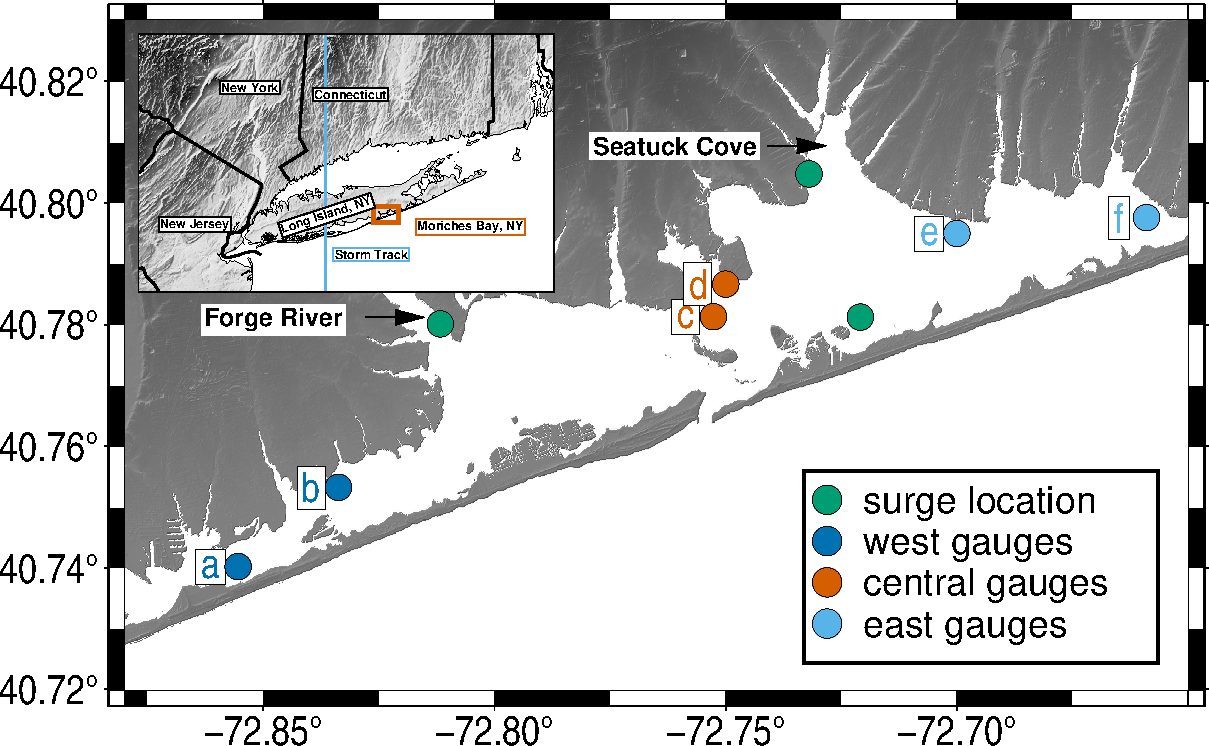
\includegraphics[width=0.95\textwidth]{figures/fig2_v2.pdf}
    \caption{Map of study area Moriches, NY. Inset shows region surrounding Moriches NY (orange box). Storm track for the 1938 Hurricane (light blue line) and our simulated storm. Green circles are locations of surge measurements from Table \ref{table:2}. Remaining circles are locations of synthetic tide gauges illustrated in Figure \ref{fig:4}}
    \label{fig:1}
\end{figure}

The 1938 Hurricane was a storm that made landfall as a category 3 hurricane near Moriches, NY on September 21, 1938. The center of the storm passed over the western side of Great South Bay, less than 75 kilometers from Moriches Bay. Figure \ref{fig:1} illustrates the location of Moriches Bay, NY and the storm track's location as it made landfall. It generated 10 breaches across the entire barrier island system bordering the south shore of Long Island, NY and caused widespread damage \citep{morang1999shinnecock, coch1994hurricane, canizares2008simulation}. Six breaches were opened during the hurricane at Moriches, NY, three west of the inlet and three east of the inlet. 

\subsection{GeoClaw}
Our goal for this project was to quantify the differences in coastal and bay flooding if breaching occurs during a hurricane. To simulate the storm we ran simulations with GeoClaw a software package that solves hyperbolic differential equations in one and two dimensions to model geophysical events \citep{clawpack, mandli2016clawpack}. Clawpack employs adaptive mesh refinement (AMR) that allows for increasing resolution where and when it is needed and reduces the computational overhead while providing an accurate solution \citep{berger2011geoclaw}. GeoClaw has been validated by the US National Tsunami Hazard Mitigation Program (NTHMP) for tsunami modeling. \citep{gonzalez2011validation} describes the benchmarking process used to validate GeoClaw. 

Storm surge modeling with GeoClaw has not been validated but has been proposed to provide a robust but less computationally expensive model than ADCIRC, a commonly utilized finite element model \citep{westerink2008basin, mandli2014adaptive}. GeoClaw calculates storm surge with a two dimensional depth averaged model that solves the classical shallow water equations with source terms for bathymetry, bottom friction, Coriolis forcing, surface pressure, and wind friction \citep{mandli2014adaptive}. GeoClaw's default storm surge modeling does not provide tidal, riverine, or wave-stress calculations that are included in other models currently used in practice, such as ADCIRC \citep{westerink2008basin, mandli2014adaptive}.

\subsection{Storm Forcing}
The storm we employed to simulate storm surge is a proxy for the 1938 New England hurricane. The storm data was generated for the US Army Corps of Engineers (USACE) North Atlantic Comprehensive Coast Survey (NACCS) \citep{cialone2015north}. The storm forcing is provided by wind and pressure fields that have data in 15 minute increments. Accurate modeling of this storm requires sub-minute data and AMR requires data to be integrated at increasing resolution where needed. To provide the sub-minute time steps we used linear interpolation of the wind and pressure fields, to define the wind and pressure forcing inside the AMR grids we employed bi-linear interpolation when and where it is required. The chosen storm has a track and intensity similar to that of the 1938 hurricane. We can verify the accuracy of the solution with a tide gauge (Station ID: 8531680) at Sandy Hook, NJ that has data recorded from 1938, once adjustments are made for modern bathymetry and sea levels \citep{coops2007}. 

\subsection{Breaching}
Breaching is a complex process that is difficult to accurately model. Storm forcing combined with barrier width, sediment transport, and other complex processes make it challenging to predict where and when a breach will occur. There is a lack of studies that document barrier island breach dimensions during storms. Due to the nature of storm induced breaching, it is difficult, if not impossible, to quantify what exactly occurs to create a breach in a barrier island during a hurricane. Lab studies of breaches in dikes provide some clues into breach formation \citep{visser1999breach}. Studies that map breach locations and dimensions usually occur well after the storm. This delay in quantifying breach dimensions does not help define initial breach width and depth as breaches will continue to grow as water passes between the ocean and back-barrier region.

\begin{equation}
    d^t = d^{t-1} - e^{-\frac{1}{2}{(X - \mu)^2}}t_T
    \label{eq:breach_gaussian}
\end{equation}

To accomplish our goal of quantifying flooding due to breaching, we chose to simplify breaching by reducing the topographic elevation of the barrier island at specific locations. We simulate a breach using an approximation of a Gaussian bell curve to provide a breach with sloping sides and the deepest part in the center. During the storm simulation we apply equation \ref{eq:breach_gaussian} to reduce the height of the barrier island at a selected location, where \emph{$\mu$} is the center of the breach location, \emph{$d^t$} is the height of the breach location at time \emph{t}, \emph{X} is the longitude of the location being reduced and \emph{$t_T$} is a timing factor that controls how quickly the breach opens. The timing factor for these simulations allows for the breach to open fully in an hour after the experiments performed by \citet{visser1999breach}. Figure \ref{fig:2} is a schematic to illustrate equation \ref{eq:breach_gaussian}.

\begin{figure}[ht]
    \centering
    \resizebox{\textwidth}{!}{%
            %% Creator: Matplotlib, PGF backend
%%
%% To include the figure in your LaTeX document, write
%%   \input{<filename>.pgf}
%%
%% Make sure the required packages are loaded in your preamble
%%   \usepackage{pgf}
%%
%% Also ensure that all the required font packages are loaded; for instance,
%% the lmodern package is sometimes necessary when using math font.
%%   \usepackage{lmodern}
%%
%% Figures using additional raster images can only be included by \input if
%% they are in the same directory as the main LaTeX file. For loading figures
%% from other directories you can use the `import` package
%%   \usepackage{import}
%%
%% and then include the figures with
%%   \import{<path to file>}{<filename>.pgf}
%%
%% Matplotlib used the following preamble
%%   \usepackage{fontspec}
%%   \setmainfont{DejaVuSerif.ttf}[Path=\detokenize{/home/catherinej/miniconda3/envs/claw/lib/python3.10/site-packages/matplotlib/mpl-data/fonts/ttf/}]
%%   \setsansfont{helvetica.ttf}[Path=\detokenize{/home/catherinej/miniconda3/envs/claw/lib/python3.10/site-packages/matplotlib/mpl-data/fonts/ttf/}]
%%   \setmonofont{DejaVuSansMono.ttf}[Path=\detokenize{/home/catherinej/miniconda3/envs/claw/lib/python3.10/site-packages/matplotlib/mpl-data/fonts/ttf/}]
%%
\begingroup%
\makeatletter%
\begin{pgfpicture}%
\pgfpathrectangle{\pgfpointorigin}{\pgfqpoint{9.008044in}{3.188875in}}%
\pgfusepath{use as bounding box, clip}%
\begin{pgfscope}%
\pgfsetbuttcap%
\pgfsetmiterjoin%
\definecolor{currentfill}{rgb}{1.000000,1.000000,1.000000}%
\pgfsetfillcolor{currentfill}%
\pgfsetlinewidth{0.000000pt}%
\definecolor{currentstroke}{rgb}{1.000000,1.000000,1.000000}%
\pgfsetstrokecolor{currentstroke}%
\pgfsetdash{}{0pt}%
\pgfpathmoveto{\pgfqpoint{0.000000in}{0.000000in}}%
\pgfpathlineto{\pgfqpoint{9.008044in}{0.000000in}}%
\pgfpathlineto{\pgfqpoint{9.008044in}{3.188875in}}%
\pgfpathlineto{\pgfqpoint{0.000000in}{3.188875in}}%
\pgfpathlineto{\pgfqpoint{0.000000in}{0.000000in}}%
\pgfpathclose%
\pgfusepath{fill}%
\end{pgfscope}%
\begin{pgfscope}%
\pgfsetbuttcap%
\pgfsetmiterjoin%
\definecolor{currentfill}{rgb}{1.000000,1.000000,1.000000}%
\pgfsetfillcolor{currentfill}%
\pgfsetlinewidth{0.000000pt}%
\definecolor{currentstroke}{rgb}{0.000000,0.000000,0.000000}%
\pgfsetstrokecolor{currentstroke}%
\pgfsetstrokeopacity{0.000000}%
\pgfsetdash{}{0pt}%
\pgfpathmoveto{\pgfqpoint{0.853515in}{0.656145in}}%
\pgfpathlineto{\pgfqpoint{3.132927in}{0.656145in}}%
\pgfpathlineto{\pgfqpoint{3.132927in}{2.846145in}}%
\pgfpathlineto{\pgfqpoint{0.853515in}{2.846145in}}%
\pgfpathlineto{\pgfqpoint{0.853515in}{0.656145in}}%
\pgfpathclose%
\pgfusepath{fill}%
\end{pgfscope}%
\begin{pgfscope}%
\pgfpathrectangle{\pgfqpoint{0.853515in}{0.656145in}}{\pgfqpoint{2.279412in}{2.190000in}}%
\pgfusepath{clip}%
\pgfsetbuttcap%
\pgfsetmiterjoin%
\definecolor{currentfill}{rgb}{0.835294,0.368627,0.000000}%
\pgfsetfillcolor{currentfill}%
\pgfsetfillopacity{0.200000}%
\pgfsetlinewidth{0.803000pt}%
\definecolor{currentstroke}{rgb}{0.000000,0.000000,0.000000}%
\pgfsetstrokecolor{currentstroke}%
\pgfsetstrokeopacity{0.200000}%
\pgfsetdash{}{0pt}%
\pgfpathmoveto{\pgfqpoint{1.160962in}{0.656145in}}%
\pgfpathlineto{\pgfqpoint{1.160962in}{1.301347in}}%
\pgfpathlineto{\pgfqpoint{1.256110in}{1.301347in}}%
\pgfpathlineto{\pgfqpoint{1.256110in}{1.144655in}}%
\pgfpathlineto{\pgfqpoint{1.351258in}{1.144655in}}%
\pgfpathlineto{\pgfqpoint{1.351258in}{1.421170in}}%
\pgfpathlineto{\pgfqpoint{1.446405in}{1.421170in}}%
\pgfpathlineto{\pgfqpoint{1.446405in}{1.172307in}}%
\pgfpathlineto{\pgfqpoint{1.541553in}{1.172307in}}%
\pgfpathlineto{\pgfqpoint{1.541553in}{0.951095in}}%
\pgfpathlineto{\pgfqpoint{1.636701in}{0.951095in}}%
\pgfpathlineto{\pgfqpoint{1.636701in}{0.683797in}}%
\pgfpathlineto{\pgfqpoint{1.731849in}{0.683797in}}%
\pgfpathlineto{\pgfqpoint{1.731849in}{0.656145in}}%
\pgfpathlineto{\pgfqpoint{1.826996in}{0.656145in}}%
\pgfpathlineto{\pgfqpoint{1.826996in}{0.656145in}}%
\pgfpathlineto{\pgfqpoint{1.922144in}{0.656145in}}%
\pgfpathlineto{\pgfqpoint{1.922144in}{0.656145in}}%
\pgfpathlineto{\pgfqpoint{2.017292in}{0.656145in}}%
\pgfpathlineto{\pgfqpoint{2.017292in}{0.656145in}}%
\pgfpathlineto{\pgfqpoint{2.112440in}{0.656145in}}%
\pgfpathlineto{\pgfqpoint{2.112440in}{0.656145in}}%
\pgfpathlineto{\pgfqpoint{2.207587in}{0.656145in}}%
\pgfpathlineto{\pgfqpoint{2.207587in}{0.656145in}}%
\pgfpathlineto{\pgfqpoint{2.302735in}{0.656145in}}%
\pgfpathlineto{\pgfqpoint{2.302735in}{0.656145in}}%
\pgfpathlineto{\pgfqpoint{2.397883in}{0.656145in}}%
\pgfpathlineto{\pgfqpoint{2.397883in}{0.656145in}}%
\pgfpathlineto{\pgfqpoint{2.493031in}{0.656145in}}%
\pgfpathlineto{\pgfqpoint{2.493031in}{0.656145in}}%
\pgfpathlineto{\pgfqpoint{2.588178in}{0.656145in}}%
\pgfpathlineto{\pgfqpoint{2.588178in}{0.656145in}}%
\pgfpathlineto{\pgfqpoint{2.683326in}{0.656145in}}%
\pgfpathlineto{\pgfqpoint{2.683326in}{0.656145in}}%
\pgfpathlineto{\pgfqpoint{2.778474in}{0.656145in}}%
\pgfpathlineto{\pgfqpoint{2.778474in}{0.656145in}}%
\pgfpathlineto{\pgfqpoint{2.873622in}{0.656145in}}%
\pgfpathlineto{\pgfqpoint{2.873622in}{0.656145in}}%
\pgfpathlineto{\pgfqpoint{2.968769in}{0.656145in}}%
\pgfpathlineto{\pgfqpoint{2.968769in}{0.656145in}}%
\pgfpathlineto{\pgfqpoint{3.063917in}{0.656145in}}%
\pgfpathlineto{\pgfqpoint{3.063917in}{0.656145in}}%
\pgfpathlineto{\pgfqpoint{2.968769in}{0.656145in}}%
\pgfpathlineto{\pgfqpoint{2.968769in}{0.656145in}}%
\pgfpathlineto{\pgfqpoint{2.873622in}{0.656145in}}%
\pgfpathlineto{\pgfqpoint{2.873622in}{0.656145in}}%
\pgfpathlineto{\pgfqpoint{2.778474in}{0.656145in}}%
\pgfpathlineto{\pgfqpoint{2.778474in}{0.656145in}}%
\pgfpathlineto{\pgfqpoint{2.683326in}{0.656145in}}%
\pgfpathlineto{\pgfqpoint{2.683326in}{0.656145in}}%
\pgfpathlineto{\pgfqpoint{2.588178in}{0.656145in}}%
\pgfpathlineto{\pgfqpoint{2.588178in}{0.656145in}}%
\pgfpathlineto{\pgfqpoint{2.493031in}{0.656145in}}%
\pgfpathlineto{\pgfqpoint{2.493031in}{0.656145in}}%
\pgfpathlineto{\pgfqpoint{2.397883in}{0.656145in}}%
\pgfpathlineto{\pgfqpoint{2.397883in}{0.656145in}}%
\pgfpathlineto{\pgfqpoint{2.302735in}{0.656145in}}%
\pgfpathlineto{\pgfqpoint{2.302735in}{0.656145in}}%
\pgfpathlineto{\pgfqpoint{2.207587in}{0.656145in}}%
\pgfpathlineto{\pgfqpoint{2.207587in}{0.656145in}}%
\pgfpathlineto{\pgfqpoint{2.112440in}{0.656145in}}%
\pgfpathlineto{\pgfqpoint{2.112440in}{0.656145in}}%
\pgfpathlineto{\pgfqpoint{2.017292in}{0.656145in}}%
\pgfpathlineto{\pgfqpoint{2.017292in}{0.656145in}}%
\pgfpathlineto{\pgfqpoint{1.922144in}{0.656145in}}%
\pgfpathlineto{\pgfqpoint{1.922144in}{0.656145in}}%
\pgfpathlineto{\pgfqpoint{1.826996in}{0.656145in}}%
\pgfpathlineto{\pgfqpoint{1.826996in}{0.656145in}}%
\pgfpathlineto{\pgfqpoint{1.731849in}{0.656145in}}%
\pgfpathlineto{\pgfqpoint{1.731849in}{0.656145in}}%
\pgfpathlineto{\pgfqpoint{1.636701in}{0.656145in}}%
\pgfpathlineto{\pgfqpoint{1.636701in}{0.656145in}}%
\pgfpathlineto{\pgfqpoint{1.541553in}{0.656145in}}%
\pgfpathlineto{\pgfqpoint{1.541553in}{0.656145in}}%
\pgfpathlineto{\pgfqpoint{1.446405in}{0.656145in}}%
\pgfpathlineto{\pgfqpoint{1.446405in}{0.656145in}}%
\pgfpathlineto{\pgfqpoint{1.351258in}{0.656145in}}%
\pgfpathlineto{\pgfqpoint{1.351258in}{0.656145in}}%
\pgfpathlineto{\pgfqpoint{1.256110in}{0.656145in}}%
\pgfpathlineto{\pgfqpoint{1.256110in}{0.656145in}}%
\pgfpathlineto{\pgfqpoint{1.160962in}{0.656145in}}%
\pgfpathclose%
\pgfusepath{stroke,fill}%
\end{pgfscope}%
\begin{pgfscope}%
\pgfpathrectangle{\pgfqpoint{0.853515in}{0.656145in}}{\pgfqpoint{2.279412in}{2.190000in}}%
\pgfusepath{clip}%
\pgfsetbuttcap%
\pgfsetmiterjoin%
\definecolor{currentfill}{rgb}{0.000000,0.619608,0.450980}%
\pgfsetfillcolor{currentfill}%
\pgfsetfillopacity{0.200000}%
\pgfsetlinewidth{0.803000pt}%
\definecolor{currentstroke}{rgb}{0.000000,0.000000,0.000000}%
\pgfsetstrokecolor{currentstroke}%
\pgfsetstrokeopacity{0.200000}%
\pgfsetdash{}{0pt}%
\pgfpathmoveto{\pgfqpoint{1.160962in}{0.656145in}}%
\pgfpathlineto{\pgfqpoint{1.160962in}{0.656145in}}%
\pgfpathlineto{\pgfqpoint{1.256110in}{0.656145in}}%
\pgfpathlineto{\pgfqpoint{1.256110in}{0.738742in}}%
\pgfpathlineto{\pgfqpoint{1.351258in}{0.738742in}}%
\pgfpathlineto{\pgfqpoint{1.351258in}{1.375919in}}%
\pgfpathlineto{\pgfqpoint{1.446405in}{1.375919in}}%
\pgfpathlineto{\pgfqpoint{1.446405in}{1.576512in}}%
\pgfpathlineto{\pgfqpoint{1.541553in}{1.576512in}}%
\pgfpathlineto{\pgfqpoint{1.541553in}{1.110429in}}%
\pgfpathlineto{\pgfqpoint{1.636701in}{1.110429in}}%
\pgfpathlineto{\pgfqpoint{1.636701in}{1.163527in}}%
\pgfpathlineto{\pgfqpoint{1.731849in}{1.163527in}}%
\pgfpathlineto{\pgfqpoint{1.731849in}{0.709243in}}%
\pgfpathlineto{\pgfqpoint{1.826996in}{0.709243in}}%
\pgfpathlineto{\pgfqpoint{1.826996in}{0.656145in}}%
\pgfpathlineto{\pgfqpoint{1.922144in}{0.656145in}}%
\pgfpathlineto{\pgfqpoint{1.922144in}{0.656145in}}%
\pgfpathlineto{\pgfqpoint{2.017292in}{0.656145in}}%
\pgfpathlineto{\pgfqpoint{2.017292in}{0.656145in}}%
\pgfpathlineto{\pgfqpoint{2.112440in}{0.656145in}}%
\pgfpathlineto{\pgfqpoint{2.112440in}{0.656145in}}%
\pgfpathlineto{\pgfqpoint{2.207587in}{0.656145in}}%
\pgfpathlineto{\pgfqpoint{2.207587in}{0.656145in}}%
\pgfpathlineto{\pgfqpoint{2.302735in}{0.656145in}}%
\pgfpathlineto{\pgfqpoint{2.302735in}{0.656145in}}%
\pgfpathlineto{\pgfqpoint{2.397883in}{0.656145in}}%
\pgfpathlineto{\pgfqpoint{2.397883in}{0.656145in}}%
\pgfpathlineto{\pgfqpoint{2.493031in}{0.656145in}}%
\pgfpathlineto{\pgfqpoint{2.493031in}{0.656145in}}%
\pgfpathlineto{\pgfqpoint{2.588178in}{0.656145in}}%
\pgfpathlineto{\pgfqpoint{2.588178in}{0.656145in}}%
\pgfpathlineto{\pgfqpoint{2.683326in}{0.656145in}}%
\pgfpathlineto{\pgfqpoint{2.683326in}{0.656145in}}%
\pgfpathlineto{\pgfqpoint{2.778474in}{0.656145in}}%
\pgfpathlineto{\pgfqpoint{2.778474in}{0.656145in}}%
\pgfpathlineto{\pgfqpoint{2.873622in}{0.656145in}}%
\pgfpathlineto{\pgfqpoint{2.873622in}{0.656145in}}%
\pgfpathlineto{\pgfqpoint{2.968769in}{0.656145in}}%
\pgfpathlineto{\pgfqpoint{2.968769in}{0.656145in}}%
\pgfpathlineto{\pgfqpoint{3.063917in}{0.656145in}}%
\pgfpathlineto{\pgfqpoint{3.063917in}{0.656145in}}%
\pgfpathlineto{\pgfqpoint{2.968769in}{0.656145in}}%
\pgfpathlineto{\pgfqpoint{2.968769in}{0.656145in}}%
\pgfpathlineto{\pgfqpoint{2.873622in}{0.656145in}}%
\pgfpathlineto{\pgfqpoint{2.873622in}{0.656145in}}%
\pgfpathlineto{\pgfqpoint{2.778474in}{0.656145in}}%
\pgfpathlineto{\pgfqpoint{2.778474in}{0.656145in}}%
\pgfpathlineto{\pgfqpoint{2.683326in}{0.656145in}}%
\pgfpathlineto{\pgfqpoint{2.683326in}{0.656145in}}%
\pgfpathlineto{\pgfqpoint{2.588178in}{0.656145in}}%
\pgfpathlineto{\pgfqpoint{2.588178in}{0.656145in}}%
\pgfpathlineto{\pgfqpoint{2.493031in}{0.656145in}}%
\pgfpathlineto{\pgfqpoint{2.493031in}{0.656145in}}%
\pgfpathlineto{\pgfqpoint{2.397883in}{0.656145in}}%
\pgfpathlineto{\pgfqpoint{2.397883in}{0.656145in}}%
\pgfpathlineto{\pgfqpoint{2.302735in}{0.656145in}}%
\pgfpathlineto{\pgfqpoint{2.302735in}{0.656145in}}%
\pgfpathlineto{\pgfqpoint{2.207587in}{0.656145in}}%
\pgfpathlineto{\pgfqpoint{2.207587in}{0.656145in}}%
\pgfpathlineto{\pgfqpoint{2.112440in}{0.656145in}}%
\pgfpathlineto{\pgfqpoint{2.112440in}{0.656145in}}%
\pgfpathlineto{\pgfqpoint{2.017292in}{0.656145in}}%
\pgfpathlineto{\pgfqpoint{2.017292in}{0.656145in}}%
\pgfpathlineto{\pgfqpoint{1.922144in}{0.656145in}}%
\pgfpathlineto{\pgfqpoint{1.922144in}{0.656145in}}%
\pgfpathlineto{\pgfqpoint{1.826996in}{0.656145in}}%
\pgfpathlineto{\pgfqpoint{1.826996in}{0.656145in}}%
\pgfpathlineto{\pgfqpoint{1.731849in}{0.656145in}}%
\pgfpathlineto{\pgfqpoint{1.731849in}{0.656145in}}%
\pgfpathlineto{\pgfqpoint{1.636701in}{0.656145in}}%
\pgfpathlineto{\pgfqpoint{1.636701in}{0.656145in}}%
\pgfpathlineto{\pgfqpoint{1.541553in}{0.656145in}}%
\pgfpathlineto{\pgfqpoint{1.541553in}{0.656145in}}%
\pgfpathlineto{\pgfqpoint{1.446405in}{0.656145in}}%
\pgfpathlineto{\pgfqpoint{1.446405in}{0.656145in}}%
\pgfpathlineto{\pgfqpoint{1.351258in}{0.656145in}}%
\pgfpathlineto{\pgfqpoint{1.351258in}{0.656145in}}%
\pgfpathlineto{\pgfqpoint{1.256110in}{0.656145in}}%
\pgfpathlineto{\pgfqpoint{1.256110in}{0.656145in}}%
\pgfpathlineto{\pgfqpoint{1.160962in}{0.656145in}}%
\pgfpathclose%
\pgfusepath{stroke,fill}%
\end{pgfscope}%
\begin{pgfscope}%
\pgfpathrectangle{\pgfqpoint{0.853515in}{0.656145in}}{\pgfqpoint{2.279412in}{2.190000in}}%
\pgfusepath{clip}%
\pgfsetbuttcap%
\pgfsetmiterjoin%
\definecolor{currentfill}{rgb}{0.337255,0.705882,0.913725}%
\pgfsetfillcolor{currentfill}%
\pgfsetfillopacity{0.200000}%
\pgfsetlinewidth{0.803000pt}%
\definecolor{currentstroke}{rgb}{0.000000,0.000000,0.000000}%
\pgfsetstrokecolor{currentstroke}%
\pgfsetstrokeopacity{0.200000}%
\pgfsetdash{}{0pt}%
\pgfpathmoveto{\pgfqpoint{1.160962in}{0.656145in}}%
\pgfpathlineto{\pgfqpoint{1.160962in}{0.656145in}}%
\pgfpathlineto{\pgfqpoint{1.256110in}{0.656145in}}%
\pgfpathlineto{\pgfqpoint{1.256110in}{0.656145in}}%
\pgfpathlineto{\pgfqpoint{1.351258in}{0.656145in}}%
\pgfpathlineto{\pgfqpoint{1.351258in}{0.656145in}}%
\pgfpathlineto{\pgfqpoint{1.446405in}{0.656145in}}%
\pgfpathlineto{\pgfqpoint{1.446405in}{0.740078in}}%
\pgfpathlineto{\pgfqpoint{1.541553in}{0.740078in}}%
\pgfpathlineto{\pgfqpoint{1.541553in}{1.411540in}}%
\pgfpathlineto{\pgfqpoint{1.636701in}{1.411540in}}%
\pgfpathlineto{\pgfqpoint{1.636701in}{2.483297in}}%
\pgfpathlineto{\pgfqpoint{1.731849in}{2.483297in}}%
\pgfpathlineto{\pgfqpoint{1.731849in}{0.727165in}}%
\pgfpathlineto{\pgfqpoint{1.826996in}{0.727165in}}%
\pgfpathlineto{\pgfqpoint{1.826996in}{0.656145in}}%
\pgfpathlineto{\pgfqpoint{1.922144in}{0.656145in}}%
\pgfpathlineto{\pgfqpoint{1.922144in}{0.656145in}}%
\pgfpathlineto{\pgfqpoint{2.017292in}{0.656145in}}%
\pgfpathlineto{\pgfqpoint{2.017292in}{0.656145in}}%
\pgfpathlineto{\pgfqpoint{2.112440in}{0.656145in}}%
\pgfpathlineto{\pgfqpoint{2.112440in}{0.656145in}}%
\pgfpathlineto{\pgfqpoint{2.207587in}{0.656145in}}%
\pgfpathlineto{\pgfqpoint{2.207587in}{0.656145in}}%
\pgfpathlineto{\pgfqpoint{2.302735in}{0.656145in}}%
\pgfpathlineto{\pgfqpoint{2.302735in}{0.656145in}}%
\pgfpathlineto{\pgfqpoint{2.397883in}{0.656145in}}%
\pgfpathlineto{\pgfqpoint{2.397883in}{0.656145in}}%
\pgfpathlineto{\pgfqpoint{2.493031in}{0.656145in}}%
\pgfpathlineto{\pgfqpoint{2.493031in}{0.656145in}}%
\pgfpathlineto{\pgfqpoint{2.588178in}{0.656145in}}%
\pgfpathlineto{\pgfqpoint{2.588178in}{0.656145in}}%
\pgfpathlineto{\pgfqpoint{2.683326in}{0.656145in}}%
\pgfpathlineto{\pgfqpoint{2.683326in}{0.656145in}}%
\pgfpathlineto{\pgfqpoint{2.778474in}{0.656145in}}%
\pgfpathlineto{\pgfqpoint{2.778474in}{0.656145in}}%
\pgfpathlineto{\pgfqpoint{2.873622in}{0.656145in}}%
\pgfpathlineto{\pgfqpoint{2.873622in}{0.656145in}}%
\pgfpathlineto{\pgfqpoint{2.968769in}{0.656145in}}%
\pgfpathlineto{\pgfqpoint{2.968769in}{0.656145in}}%
\pgfpathlineto{\pgfqpoint{3.063917in}{0.656145in}}%
\pgfpathlineto{\pgfqpoint{3.063917in}{0.656145in}}%
\pgfpathlineto{\pgfqpoint{2.968769in}{0.656145in}}%
\pgfpathlineto{\pgfqpoint{2.968769in}{0.656145in}}%
\pgfpathlineto{\pgfqpoint{2.873622in}{0.656145in}}%
\pgfpathlineto{\pgfqpoint{2.873622in}{0.656145in}}%
\pgfpathlineto{\pgfqpoint{2.778474in}{0.656145in}}%
\pgfpathlineto{\pgfqpoint{2.778474in}{0.656145in}}%
\pgfpathlineto{\pgfqpoint{2.683326in}{0.656145in}}%
\pgfpathlineto{\pgfqpoint{2.683326in}{0.656145in}}%
\pgfpathlineto{\pgfqpoint{2.588178in}{0.656145in}}%
\pgfpathlineto{\pgfqpoint{2.588178in}{0.656145in}}%
\pgfpathlineto{\pgfqpoint{2.493031in}{0.656145in}}%
\pgfpathlineto{\pgfqpoint{2.493031in}{0.656145in}}%
\pgfpathlineto{\pgfqpoint{2.397883in}{0.656145in}}%
\pgfpathlineto{\pgfqpoint{2.397883in}{0.656145in}}%
\pgfpathlineto{\pgfqpoint{2.302735in}{0.656145in}}%
\pgfpathlineto{\pgfqpoint{2.302735in}{0.656145in}}%
\pgfpathlineto{\pgfqpoint{2.207587in}{0.656145in}}%
\pgfpathlineto{\pgfqpoint{2.207587in}{0.656145in}}%
\pgfpathlineto{\pgfqpoint{2.112440in}{0.656145in}}%
\pgfpathlineto{\pgfqpoint{2.112440in}{0.656145in}}%
\pgfpathlineto{\pgfqpoint{2.017292in}{0.656145in}}%
\pgfpathlineto{\pgfqpoint{2.017292in}{0.656145in}}%
\pgfpathlineto{\pgfqpoint{1.922144in}{0.656145in}}%
\pgfpathlineto{\pgfqpoint{1.922144in}{0.656145in}}%
\pgfpathlineto{\pgfqpoint{1.826996in}{0.656145in}}%
\pgfpathlineto{\pgfqpoint{1.826996in}{0.656145in}}%
\pgfpathlineto{\pgfqpoint{1.731849in}{0.656145in}}%
\pgfpathlineto{\pgfqpoint{1.731849in}{0.656145in}}%
\pgfpathlineto{\pgfqpoint{1.636701in}{0.656145in}}%
\pgfpathlineto{\pgfqpoint{1.636701in}{0.656145in}}%
\pgfpathlineto{\pgfqpoint{1.541553in}{0.656145in}}%
\pgfpathlineto{\pgfqpoint{1.541553in}{0.656145in}}%
\pgfpathlineto{\pgfqpoint{1.446405in}{0.656145in}}%
\pgfpathlineto{\pgfqpoint{1.446405in}{0.656145in}}%
\pgfpathlineto{\pgfqpoint{1.351258in}{0.656145in}}%
\pgfpathlineto{\pgfqpoint{1.351258in}{0.656145in}}%
\pgfpathlineto{\pgfqpoint{1.256110in}{0.656145in}}%
\pgfpathlineto{\pgfqpoint{1.256110in}{0.656145in}}%
\pgfpathlineto{\pgfqpoint{1.160962in}{0.656145in}}%
\pgfpathclose%
\pgfusepath{stroke,fill}%
\end{pgfscope}%
\begin{pgfscope}%
\pgfpathrectangle{\pgfqpoint{0.853515in}{0.656145in}}{\pgfqpoint{2.279412in}{2.190000in}}%
\pgfusepath{clip}%
\pgfsetbuttcap%
\pgfsetmiterjoin%
\definecolor{currentfill}{rgb}{0.800000,0.474510,0.654902}%
\pgfsetfillcolor{currentfill}%
\pgfsetfillopacity{0.200000}%
\pgfsetlinewidth{0.803000pt}%
\definecolor{currentstroke}{rgb}{0.000000,0.000000,0.000000}%
\pgfsetstrokecolor{currentstroke}%
\pgfsetstrokeopacity{0.200000}%
\pgfsetdash{}{0pt}%
\pgfpathmoveto{\pgfqpoint{1.160962in}{0.656145in}}%
\pgfpathlineto{\pgfqpoint{1.160962in}{0.716979in}}%
\pgfpathlineto{\pgfqpoint{1.256110in}{0.716979in}}%
\pgfpathlineto{\pgfqpoint{1.256110in}{0.716979in}}%
\pgfpathlineto{\pgfqpoint{1.351258in}{0.716979in}}%
\pgfpathlineto{\pgfqpoint{1.351258in}{0.708288in}}%
\pgfpathlineto{\pgfqpoint{1.446405in}{0.708288in}}%
\pgfpathlineto{\pgfqpoint{1.446405in}{0.682217in}}%
\pgfpathlineto{\pgfqpoint{1.541553in}{0.682217in}}%
\pgfpathlineto{\pgfqpoint{1.541553in}{0.734359in}}%
\pgfpathlineto{\pgfqpoint{1.636701in}{0.734359in}}%
\pgfpathlineto{\pgfqpoint{1.636701in}{0.664836in}}%
\pgfpathlineto{\pgfqpoint{1.731849in}{0.664836in}}%
\pgfpathlineto{\pgfqpoint{1.731849in}{0.716979in}}%
\pgfpathlineto{\pgfqpoint{1.826996in}{0.716979in}}%
\pgfpathlineto{\pgfqpoint{1.826996in}{0.725669in}}%
\pgfpathlineto{\pgfqpoint{1.922144in}{0.725669in}}%
\pgfpathlineto{\pgfqpoint{1.922144in}{0.725669in}}%
\pgfpathlineto{\pgfqpoint{2.017292in}{0.725669in}}%
\pgfpathlineto{\pgfqpoint{2.017292in}{0.725669in}}%
\pgfpathlineto{\pgfqpoint{2.112440in}{0.725669in}}%
\pgfpathlineto{\pgfqpoint{2.112440in}{0.786502in}}%
\pgfpathlineto{\pgfqpoint{2.207587in}{0.786502in}}%
\pgfpathlineto{\pgfqpoint{2.207587in}{0.769121in}}%
\pgfpathlineto{\pgfqpoint{2.302735in}{0.769121in}}%
\pgfpathlineto{\pgfqpoint{2.302735in}{0.829955in}}%
\pgfpathlineto{\pgfqpoint{2.397883in}{0.829955in}}%
\pgfpathlineto{\pgfqpoint{2.397883in}{0.777812in}}%
\pgfpathlineto{\pgfqpoint{2.493031in}{0.777812in}}%
\pgfpathlineto{\pgfqpoint{2.493031in}{0.838645in}}%
\pgfpathlineto{\pgfqpoint{2.588178in}{0.838645in}}%
\pgfpathlineto{\pgfqpoint{2.588178in}{0.812574in}}%
\pgfpathlineto{\pgfqpoint{2.683326in}{0.812574in}}%
\pgfpathlineto{\pgfqpoint{2.683326in}{0.795193in}}%
\pgfpathlineto{\pgfqpoint{2.778474in}{0.795193in}}%
\pgfpathlineto{\pgfqpoint{2.778474in}{0.856026in}}%
\pgfpathlineto{\pgfqpoint{2.873622in}{0.856026in}}%
\pgfpathlineto{\pgfqpoint{2.873622in}{1.203645in}}%
\pgfpathlineto{\pgfqpoint{2.968769in}{1.203645in}}%
\pgfpathlineto{\pgfqpoint{2.968769in}{1.073288in}}%
\pgfpathlineto{\pgfqpoint{3.063917in}{1.073288in}}%
\pgfpathlineto{\pgfqpoint{3.063917in}{0.656145in}}%
\pgfpathlineto{\pgfqpoint{2.968769in}{0.656145in}}%
\pgfpathlineto{\pgfqpoint{2.968769in}{0.656145in}}%
\pgfpathlineto{\pgfqpoint{2.873622in}{0.656145in}}%
\pgfpathlineto{\pgfqpoint{2.873622in}{0.656145in}}%
\pgfpathlineto{\pgfqpoint{2.778474in}{0.656145in}}%
\pgfpathlineto{\pgfqpoint{2.778474in}{0.656145in}}%
\pgfpathlineto{\pgfqpoint{2.683326in}{0.656145in}}%
\pgfpathlineto{\pgfqpoint{2.683326in}{0.656145in}}%
\pgfpathlineto{\pgfqpoint{2.588178in}{0.656145in}}%
\pgfpathlineto{\pgfqpoint{2.588178in}{0.656145in}}%
\pgfpathlineto{\pgfqpoint{2.493031in}{0.656145in}}%
\pgfpathlineto{\pgfqpoint{2.493031in}{0.656145in}}%
\pgfpathlineto{\pgfqpoint{2.397883in}{0.656145in}}%
\pgfpathlineto{\pgfqpoint{2.397883in}{0.656145in}}%
\pgfpathlineto{\pgfqpoint{2.302735in}{0.656145in}}%
\pgfpathlineto{\pgfqpoint{2.302735in}{0.656145in}}%
\pgfpathlineto{\pgfqpoint{2.207587in}{0.656145in}}%
\pgfpathlineto{\pgfqpoint{2.207587in}{0.656145in}}%
\pgfpathlineto{\pgfqpoint{2.112440in}{0.656145in}}%
\pgfpathlineto{\pgfqpoint{2.112440in}{0.656145in}}%
\pgfpathlineto{\pgfqpoint{2.017292in}{0.656145in}}%
\pgfpathlineto{\pgfqpoint{2.017292in}{0.656145in}}%
\pgfpathlineto{\pgfqpoint{1.922144in}{0.656145in}}%
\pgfpathlineto{\pgfqpoint{1.922144in}{0.656145in}}%
\pgfpathlineto{\pgfqpoint{1.826996in}{0.656145in}}%
\pgfpathlineto{\pgfqpoint{1.826996in}{0.656145in}}%
\pgfpathlineto{\pgfqpoint{1.731849in}{0.656145in}}%
\pgfpathlineto{\pgfqpoint{1.731849in}{0.656145in}}%
\pgfpathlineto{\pgfqpoint{1.636701in}{0.656145in}}%
\pgfpathlineto{\pgfqpoint{1.636701in}{0.656145in}}%
\pgfpathlineto{\pgfqpoint{1.541553in}{0.656145in}}%
\pgfpathlineto{\pgfqpoint{1.541553in}{0.656145in}}%
\pgfpathlineto{\pgfqpoint{1.446405in}{0.656145in}}%
\pgfpathlineto{\pgfqpoint{1.446405in}{0.656145in}}%
\pgfpathlineto{\pgfqpoint{1.351258in}{0.656145in}}%
\pgfpathlineto{\pgfqpoint{1.351258in}{0.656145in}}%
\pgfpathlineto{\pgfqpoint{1.256110in}{0.656145in}}%
\pgfpathlineto{\pgfqpoint{1.256110in}{0.656145in}}%
\pgfpathlineto{\pgfqpoint{1.160962in}{0.656145in}}%
\pgfpathclose%
\pgfusepath{stroke,fill}%
\end{pgfscope}%
\begin{pgfscope}%
\pgfsetbuttcap%
\pgfsetroundjoin%
\definecolor{currentfill}{rgb}{0.196078,0.188235,0.203922}%
\pgfsetfillcolor{currentfill}%
\pgfsetlinewidth{0.803000pt}%
\definecolor{currentstroke}{rgb}{0.196078,0.188235,0.203922}%
\pgfsetstrokecolor{currentstroke}%
\pgfsetdash{}{0pt}%
\pgfsys@defobject{currentmarker}{\pgfqpoint{0.000000in}{-0.048611in}}{\pgfqpoint{0.000000in}{0.000000in}}{%
\pgfpathmoveto{\pgfqpoint{0.000000in}{0.000000in}}%
\pgfpathlineto{\pgfqpoint{0.000000in}{-0.048611in}}%
\pgfusepath{stroke,fill}%
}%
\begin{pgfscope}%
\pgfsys@transformshift{0.853515in}{0.656145in}%
\pgfsys@useobject{currentmarker}{}%
\end{pgfscope}%
\end{pgfscope}%
\begin{pgfscope}%
\definecolor{textcolor}{rgb}{0.196078,0.188235,0.203922}%
\pgfsetstrokecolor{textcolor}%
\pgfsetfillcolor{textcolor}%
\pgftext[x=0.853515in,y=0.558923in,,top]{\color{textcolor}\sffamily\fontsize{10.000000}{12.000000}\selectfont 0.55}%
\end{pgfscope}%
\begin{pgfscope}%
\pgfsetbuttcap%
\pgfsetroundjoin%
\definecolor{currentfill}{rgb}{0.196078,0.188235,0.203922}%
\pgfsetfillcolor{currentfill}%
\pgfsetlinewidth{0.803000pt}%
\definecolor{currentstroke}{rgb}{0.196078,0.188235,0.203922}%
\pgfsetstrokecolor{currentstroke}%
\pgfsetdash{}{0pt}%
\pgfsys@defobject{currentmarker}{\pgfqpoint{0.000000in}{-0.048611in}}{\pgfqpoint{0.000000in}{0.000000in}}{%
\pgfpathmoveto{\pgfqpoint{0.000000in}{0.000000in}}%
\pgfpathlineto{\pgfqpoint{0.000000in}{-0.048611in}}%
\pgfusepath{stroke,fill}%
}%
\begin{pgfscope}%
\pgfsys@transformshift{1.179146in}{0.656145in}%
\pgfsys@useobject{currentmarker}{}%
\end{pgfscope}%
\end{pgfscope}%
\begin{pgfscope}%
\definecolor{textcolor}{rgb}{0.196078,0.188235,0.203922}%
\pgfsetstrokecolor{textcolor}%
\pgfsetfillcolor{textcolor}%
\pgftext[x=1.179146in,y=0.558923in,,top]{\color{textcolor}\sffamily\fontsize{10.000000}{12.000000}\selectfont 0.76}%
\end{pgfscope}%
\begin{pgfscope}%
\pgfsetbuttcap%
\pgfsetroundjoin%
\definecolor{currentfill}{rgb}{0.196078,0.188235,0.203922}%
\pgfsetfillcolor{currentfill}%
\pgfsetlinewidth{0.803000pt}%
\definecolor{currentstroke}{rgb}{0.196078,0.188235,0.203922}%
\pgfsetstrokecolor{currentstroke}%
\pgfsetdash{}{0pt}%
\pgfsys@defobject{currentmarker}{\pgfqpoint{0.000000in}{-0.048611in}}{\pgfqpoint{0.000000in}{0.000000in}}{%
\pgfpathmoveto{\pgfqpoint{0.000000in}{0.000000in}}%
\pgfpathlineto{\pgfqpoint{0.000000in}{-0.048611in}}%
\pgfusepath{stroke,fill}%
}%
\begin{pgfscope}%
\pgfsys@transformshift{1.504776in}{0.656145in}%
\pgfsys@useobject{currentmarker}{}%
\end{pgfscope}%
\end{pgfscope}%
\begin{pgfscope}%
\definecolor{textcolor}{rgb}{0.196078,0.188235,0.203922}%
\pgfsetstrokecolor{textcolor}%
\pgfsetfillcolor{textcolor}%
\pgftext[x=1.504776in,y=0.558923in,,top]{\color{textcolor}\sffamily\fontsize{10.000000}{12.000000}\selectfont 0.96}%
\end{pgfscope}%
\begin{pgfscope}%
\pgfsetbuttcap%
\pgfsetroundjoin%
\definecolor{currentfill}{rgb}{0.196078,0.188235,0.203922}%
\pgfsetfillcolor{currentfill}%
\pgfsetlinewidth{0.803000pt}%
\definecolor{currentstroke}{rgb}{0.196078,0.188235,0.203922}%
\pgfsetstrokecolor{currentstroke}%
\pgfsetdash{}{0pt}%
\pgfsys@defobject{currentmarker}{\pgfqpoint{0.000000in}{-0.048611in}}{\pgfqpoint{0.000000in}{0.000000in}}{%
\pgfpathmoveto{\pgfqpoint{0.000000in}{0.000000in}}%
\pgfpathlineto{\pgfqpoint{0.000000in}{-0.048611in}}%
\pgfusepath{stroke,fill}%
}%
\begin{pgfscope}%
\pgfsys@transformshift{1.830406in}{0.656145in}%
\pgfsys@useobject{currentmarker}{}%
\end{pgfscope}%
\end{pgfscope}%
\begin{pgfscope}%
\definecolor{textcolor}{rgb}{0.196078,0.188235,0.203922}%
\pgfsetstrokecolor{textcolor}%
\pgfsetfillcolor{textcolor}%
\pgftext[x=1.830406in,y=0.558923in,,top]{\color{textcolor}\sffamily\fontsize{10.000000}{12.000000}\selectfont 1.17}%
\end{pgfscope}%
\begin{pgfscope}%
\pgfsetbuttcap%
\pgfsetroundjoin%
\definecolor{currentfill}{rgb}{0.196078,0.188235,0.203922}%
\pgfsetfillcolor{currentfill}%
\pgfsetlinewidth{0.803000pt}%
\definecolor{currentstroke}{rgb}{0.196078,0.188235,0.203922}%
\pgfsetstrokecolor{currentstroke}%
\pgfsetdash{}{0pt}%
\pgfsys@defobject{currentmarker}{\pgfqpoint{0.000000in}{-0.048611in}}{\pgfqpoint{0.000000in}{0.000000in}}{%
\pgfpathmoveto{\pgfqpoint{0.000000in}{0.000000in}}%
\pgfpathlineto{\pgfqpoint{0.000000in}{-0.048611in}}%
\pgfusepath{stroke,fill}%
}%
\begin{pgfscope}%
\pgfsys@transformshift{2.156036in}{0.656145in}%
\pgfsys@useobject{currentmarker}{}%
\end{pgfscope}%
\end{pgfscope}%
\begin{pgfscope}%
\definecolor{textcolor}{rgb}{0.196078,0.188235,0.203922}%
\pgfsetstrokecolor{textcolor}%
\pgfsetfillcolor{textcolor}%
\pgftext[x=2.156036in,y=0.558923in,,top]{\color{textcolor}\sffamily\fontsize{10.000000}{12.000000}\selectfont 1.38}%
\end{pgfscope}%
\begin{pgfscope}%
\pgfsetbuttcap%
\pgfsetroundjoin%
\definecolor{currentfill}{rgb}{0.196078,0.188235,0.203922}%
\pgfsetfillcolor{currentfill}%
\pgfsetlinewidth{0.803000pt}%
\definecolor{currentstroke}{rgb}{0.196078,0.188235,0.203922}%
\pgfsetstrokecolor{currentstroke}%
\pgfsetdash{}{0pt}%
\pgfsys@defobject{currentmarker}{\pgfqpoint{0.000000in}{-0.048611in}}{\pgfqpoint{0.000000in}{0.000000in}}{%
\pgfpathmoveto{\pgfqpoint{0.000000in}{0.000000in}}%
\pgfpathlineto{\pgfqpoint{0.000000in}{-0.048611in}}%
\pgfusepath{stroke,fill}%
}%
\begin{pgfscope}%
\pgfsys@transformshift{2.481667in}{0.656145in}%
\pgfsys@useobject{currentmarker}{}%
\end{pgfscope}%
\end{pgfscope}%
\begin{pgfscope}%
\definecolor{textcolor}{rgb}{0.196078,0.188235,0.203922}%
\pgfsetstrokecolor{textcolor}%
\pgfsetfillcolor{textcolor}%
\pgftext[x=2.481667in,y=0.558923in,,top]{\color{textcolor}\sffamily\fontsize{10.000000}{12.000000}\selectfont 1.59}%
\end{pgfscope}%
\begin{pgfscope}%
\pgfsetbuttcap%
\pgfsetroundjoin%
\definecolor{currentfill}{rgb}{0.196078,0.188235,0.203922}%
\pgfsetfillcolor{currentfill}%
\pgfsetlinewidth{0.803000pt}%
\definecolor{currentstroke}{rgb}{0.196078,0.188235,0.203922}%
\pgfsetstrokecolor{currentstroke}%
\pgfsetdash{}{0pt}%
\pgfsys@defobject{currentmarker}{\pgfqpoint{0.000000in}{-0.048611in}}{\pgfqpoint{0.000000in}{0.000000in}}{%
\pgfpathmoveto{\pgfqpoint{0.000000in}{0.000000in}}%
\pgfpathlineto{\pgfqpoint{0.000000in}{-0.048611in}}%
\pgfusepath{stroke,fill}%
}%
\begin{pgfscope}%
\pgfsys@transformshift{2.807297in}{0.656145in}%
\pgfsys@useobject{currentmarker}{}%
\end{pgfscope}%
\end{pgfscope}%
\begin{pgfscope}%
\definecolor{textcolor}{rgb}{0.196078,0.188235,0.203922}%
\pgfsetstrokecolor{textcolor}%
\pgfsetfillcolor{textcolor}%
\pgftext[x=2.807297in,y=0.558923in,,top]{\color{textcolor}\sffamily\fontsize{10.000000}{12.000000}\selectfont 1.79}%
\end{pgfscope}%
\begin{pgfscope}%
\pgfsetbuttcap%
\pgfsetroundjoin%
\definecolor{currentfill}{rgb}{0.196078,0.188235,0.203922}%
\pgfsetfillcolor{currentfill}%
\pgfsetlinewidth{0.803000pt}%
\definecolor{currentstroke}{rgb}{0.196078,0.188235,0.203922}%
\pgfsetstrokecolor{currentstroke}%
\pgfsetdash{}{0pt}%
\pgfsys@defobject{currentmarker}{\pgfqpoint{0.000000in}{-0.048611in}}{\pgfqpoint{0.000000in}{0.000000in}}{%
\pgfpathmoveto{\pgfqpoint{0.000000in}{0.000000in}}%
\pgfpathlineto{\pgfqpoint{0.000000in}{-0.048611in}}%
\pgfusepath{stroke,fill}%
}%
\begin{pgfscope}%
\pgfsys@transformshift{3.132927in}{0.656145in}%
\pgfsys@useobject{currentmarker}{}%
\end{pgfscope}%
\end{pgfscope}%
\begin{pgfscope}%
\definecolor{textcolor}{rgb}{0.196078,0.188235,0.203922}%
\pgfsetstrokecolor{textcolor}%
\pgfsetfillcolor{textcolor}%
\pgftext[x=3.132927in,y=0.558923in,,top]{\color{textcolor}\sffamily\fontsize{10.000000}{12.000000}\selectfont 2.00}%
\end{pgfscope}%
\begin{pgfscope}%
\pgfsetbuttcap%
\pgfsetroundjoin%
\definecolor{currentfill}{rgb}{0.196078,0.188235,0.203922}%
\pgfsetfillcolor{currentfill}%
\pgfsetlinewidth{0.803000pt}%
\definecolor{currentstroke}{rgb}{0.196078,0.188235,0.203922}%
\pgfsetstrokecolor{currentstroke}%
\pgfsetdash{}{0pt}%
\pgfsys@defobject{currentmarker}{\pgfqpoint{-0.048611in}{0.000000in}}{\pgfqpoint{-0.000000in}{0.000000in}}{%
\pgfpathmoveto{\pgfqpoint{-0.000000in}{0.000000in}}%
\pgfpathlineto{\pgfqpoint{-0.048611in}{0.000000in}}%
\pgfusepath{stroke,fill}%
}%
\begin{pgfscope}%
\pgfsys@transformshift{0.853515in}{0.656145in}%
\pgfsys@useobject{currentmarker}{}%
\end{pgfscope}%
\end{pgfscope}%
\begin{pgfscope}%
\definecolor{textcolor}{rgb}{0.196078,0.188235,0.203922}%
\pgfsetstrokecolor{textcolor}%
\pgfsetfillcolor{textcolor}%
\pgftext[x=0.578824in, y=0.606334in, left, base]{\color{textcolor}\sffamily\fontsize{10.000000}{12.000000}\selectfont \(\displaystyle {0.0}\)}%
\end{pgfscope}%
\begin{pgfscope}%
\pgfsetbuttcap%
\pgfsetroundjoin%
\definecolor{currentfill}{rgb}{0.196078,0.188235,0.203922}%
\pgfsetfillcolor{currentfill}%
\pgfsetlinewidth{0.803000pt}%
\definecolor{currentstroke}{rgb}{0.196078,0.188235,0.203922}%
\pgfsetstrokecolor{currentstroke}%
\pgfsetdash{}{0pt}%
\pgfsys@defobject{currentmarker}{\pgfqpoint{-0.048611in}{0.000000in}}{\pgfqpoint{-0.000000in}{0.000000in}}{%
\pgfpathmoveto{\pgfqpoint{-0.000000in}{0.000000in}}%
\pgfpathlineto{\pgfqpoint{-0.048611in}{0.000000in}}%
\pgfusepath{stroke,fill}%
}%
\begin{pgfscope}%
\pgfsys@transformshift{0.853515in}{1.203645in}%
\pgfsys@useobject{currentmarker}{}%
\end{pgfscope}%
\end{pgfscope}%
\begin{pgfscope}%
\definecolor{textcolor}{rgb}{0.196078,0.188235,0.203922}%
\pgfsetstrokecolor{textcolor}%
\pgfsetfillcolor{textcolor}%
\pgftext[x=0.578824in, y=1.153834in, left, base]{\color{textcolor}\sffamily\fontsize{10.000000}{12.000000}\selectfont \(\displaystyle {0.2}\)}%
\end{pgfscope}%
\begin{pgfscope}%
\pgfsetbuttcap%
\pgfsetroundjoin%
\definecolor{currentfill}{rgb}{0.196078,0.188235,0.203922}%
\pgfsetfillcolor{currentfill}%
\pgfsetlinewidth{0.803000pt}%
\definecolor{currentstroke}{rgb}{0.196078,0.188235,0.203922}%
\pgfsetstrokecolor{currentstroke}%
\pgfsetdash{}{0pt}%
\pgfsys@defobject{currentmarker}{\pgfqpoint{-0.048611in}{0.000000in}}{\pgfqpoint{-0.000000in}{0.000000in}}{%
\pgfpathmoveto{\pgfqpoint{-0.000000in}{0.000000in}}%
\pgfpathlineto{\pgfqpoint{-0.048611in}{0.000000in}}%
\pgfusepath{stroke,fill}%
}%
\begin{pgfscope}%
\pgfsys@transformshift{0.853515in}{1.751145in}%
\pgfsys@useobject{currentmarker}{}%
\end{pgfscope}%
\end{pgfscope}%
\begin{pgfscope}%
\definecolor{textcolor}{rgb}{0.196078,0.188235,0.203922}%
\pgfsetstrokecolor{textcolor}%
\pgfsetfillcolor{textcolor}%
\pgftext[x=0.578824in, y=1.701334in, left, base]{\color{textcolor}\sffamily\fontsize{10.000000}{12.000000}\selectfont \(\displaystyle {0.4}\)}%
\end{pgfscope}%
\begin{pgfscope}%
\pgfsetbuttcap%
\pgfsetroundjoin%
\definecolor{currentfill}{rgb}{0.196078,0.188235,0.203922}%
\pgfsetfillcolor{currentfill}%
\pgfsetlinewidth{0.803000pt}%
\definecolor{currentstroke}{rgb}{0.196078,0.188235,0.203922}%
\pgfsetstrokecolor{currentstroke}%
\pgfsetdash{}{0pt}%
\pgfsys@defobject{currentmarker}{\pgfqpoint{-0.048611in}{0.000000in}}{\pgfqpoint{-0.000000in}{0.000000in}}{%
\pgfpathmoveto{\pgfqpoint{-0.000000in}{0.000000in}}%
\pgfpathlineto{\pgfqpoint{-0.048611in}{0.000000in}}%
\pgfusepath{stroke,fill}%
}%
\begin{pgfscope}%
\pgfsys@transformshift{0.853515in}{2.298645in}%
\pgfsys@useobject{currentmarker}{}%
\end{pgfscope}%
\end{pgfscope}%
\begin{pgfscope}%
\definecolor{textcolor}{rgb}{0.196078,0.188235,0.203922}%
\pgfsetstrokecolor{textcolor}%
\pgfsetfillcolor{textcolor}%
\pgftext[x=0.578824in, y=2.248834in, left, base]{\color{textcolor}\sffamily\fontsize{10.000000}{12.000000}\selectfont \(\displaystyle {0.6}\)}%
\end{pgfscope}%
\begin{pgfscope}%
\pgfsetbuttcap%
\pgfsetroundjoin%
\definecolor{currentfill}{rgb}{0.196078,0.188235,0.203922}%
\pgfsetfillcolor{currentfill}%
\pgfsetlinewidth{0.803000pt}%
\definecolor{currentstroke}{rgb}{0.196078,0.188235,0.203922}%
\pgfsetstrokecolor{currentstroke}%
\pgfsetdash{}{0pt}%
\pgfsys@defobject{currentmarker}{\pgfqpoint{-0.048611in}{0.000000in}}{\pgfqpoint{-0.000000in}{0.000000in}}{%
\pgfpathmoveto{\pgfqpoint{-0.000000in}{0.000000in}}%
\pgfpathlineto{\pgfqpoint{-0.048611in}{0.000000in}}%
\pgfusepath{stroke,fill}%
}%
\begin{pgfscope}%
\pgfsys@transformshift{0.853515in}{2.846145in}%
\pgfsys@useobject{currentmarker}{}%
\end{pgfscope}%
\end{pgfscope}%
\begin{pgfscope}%
\definecolor{textcolor}{rgb}{0.196078,0.188235,0.203922}%
\pgfsetstrokecolor{textcolor}%
\pgfsetfillcolor{textcolor}%
\pgftext[x=0.578824in, y=2.796334in, left, base]{\color{textcolor}\sffamily\fontsize{10.000000}{12.000000}\selectfont \(\displaystyle {0.8}\)}%
\end{pgfscope}%
\begin{pgfscope}%
\pgfpathrectangle{\pgfqpoint{0.853515in}{0.656145in}}{\pgfqpoint{2.279412in}{2.190000in}}%
\pgfusepath{clip}%
\pgfsetbuttcap%
\pgfsetmiterjoin%
\pgfsetlinewidth{0.803000pt}%
\definecolor{currentstroke}{rgb}{0.835294,0.368627,0.000000}%
\pgfsetstrokecolor{currentstroke}%
\pgfsetstrokeopacity{0.700000}%
\pgfsetdash{}{0pt}%
\pgfpathmoveto{\pgfqpoint{1.160962in}{0.656145in}}%
\pgfpathlineto{\pgfqpoint{1.160962in}{1.301347in}}%
\pgfpathlineto{\pgfqpoint{1.256110in}{1.301347in}}%
\pgfpathlineto{\pgfqpoint{1.256110in}{1.144655in}}%
\pgfpathlineto{\pgfqpoint{1.351258in}{1.144655in}}%
\pgfpathlineto{\pgfqpoint{1.351258in}{1.421170in}}%
\pgfpathlineto{\pgfqpoint{1.446405in}{1.421170in}}%
\pgfpathlineto{\pgfqpoint{1.446405in}{1.172307in}}%
\pgfpathlineto{\pgfqpoint{1.541553in}{1.172307in}}%
\pgfpathlineto{\pgfqpoint{1.541553in}{0.951095in}}%
\pgfpathlineto{\pgfqpoint{1.636701in}{0.951095in}}%
\pgfpathlineto{\pgfqpoint{1.636701in}{0.683797in}}%
\pgfpathlineto{\pgfqpoint{1.731849in}{0.683797in}}%
\pgfpathlineto{\pgfqpoint{1.731849in}{0.656145in}}%
\pgfpathlineto{\pgfqpoint{1.826996in}{0.656145in}}%
\pgfpathlineto{\pgfqpoint{1.826996in}{0.656145in}}%
\pgfpathlineto{\pgfqpoint{1.922144in}{0.656145in}}%
\pgfpathlineto{\pgfqpoint{1.922144in}{0.656145in}}%
\pgfpathlineto{\pgfqpoint{2.017292in}{0.656145in}}%
\pgfpathlineto{\pgfqpoint{2.017292in}{0.656145in}}%
\pgfpathlineto{\pgfqpoint{2.112440in}{0.656145in}}%
\pgfpathlineto{\pgfqpoint{2.112440in}{0.656145in}}%
\pgfpathlineto{\pgfqpoint{2.207587in}{0.656145in}}%
\pgfpathlineto{\pgfqpoint{2.207587in}{0.656145in}}%
\pgfpathlineto{\pgfqpoint{2.302735in}{0.656145in}}%
\pgfpathlineto{\pgfqpoint{2.302735in}{0.656145in}}%
\pgfpathlineto{\pgfqpoint{2.397883in}{0.656145in}}%
\pgfpathlineto{\pgfqpoint{2.397883in}{0.656145in}}%
\pgfpathlineto{\pgfqpoint{2.493031in}{0.656145in}}%
\pgfpathlineto{\pgfqpoint{2.493031in}{0.656145in}}%
\pgfpathlineto{\pgfqpoint{2.588178in}{0.656145in}}%
\pgfpathlineto{\pgfqpoint{2.588178in}{0.656145in}}%
\pgfpathlineto{\pgfqpoint{2.683326in}{0.656145in}}%
\pgfpathlineto{\pgfqpoint{2.683326in}{0.656145in}}%
\pgfpathlineto{\pgfqpoint{2.778474in}{0.656145in}}%
\pgfpathlineto{\pgfqpoint{2.778474in}{0.656145in}}%
\pgfpathlineto{\pgfqpoint{2.873622in}{0.656145in}}%
\pgfpathlineto{\pgfqpoint{2.873622in}{0.656145in}}%
\pgfpathlineto{\pgfqpoint{2.968769in}{0.656145in}}%
\pgfpathlineto{\pgfqpoint{2.968769in}{0.656145in}}%
\pgfpathlineto{\pgfqpoint{3.063917in}{0.656145in}}%
\pgfpathlineto{\pgfqpoint{3.063917in}{0.656145in}}%
\pgfusepath{stroke}%
\end{pgfscope}%
\begin{pgfscope}%
\pgfpathrectangle{\pgfqpoint{0.853515in}{0.656145in}}{\pgfqpoint{2.279412in}{2.190000in}}%
\pgfusepath{clip}%
\pgfsetbuttcap%
\pgfsetmiterjoin%
\pgfsetlinewidth{0.803000pt}%
\definecolor{currentstroke}{rgb}{0.000000,0.619608,0.450980}%
\pgfsetstrokecolor{currentstroke}%
\pgfsetstrokeopacity{0.700000}%
\pgfsetdash{}{0pt}%
\pgfpathmoveto{\pgfqpoint{1.160962in}{0.656145in}}%
\pgfpathlineto{\pgfqpoint{1.160962in}{0.656145in}}%
\pgfpathlineto{\pgfqpoint{1.256110in}{0.656145in}}%
\pgfpathlineto{\pgfqpoint{1.256110in}{0.738742in}}%
\pgfpathlineto{\pgfqpoint{1.351258in}{0.738742in}}%
\pgfpathlineto{\pgfqpoint{1.351258in}{1.375919in}}%
\pgfpathlineto{\pgfqpoint{1.446405in}{1.375919in}}%
\pgfpathlineto{\pgfqpoint{1.446405in}{1.576512in}}%
\pgfpathlineto{\pgfqpoint{1.541553in}{1.576512in}}%
\pgfpathlineto{\pgfqpoint{1.541553in}{1.110429in}}%
\pgfpathlineto{\pgfqpoint{1.636701in}{1.110429in}}%
\pgfpathlineto{\pgfqpoint{1.636701in}{1.163527in}}%
\pgfpathlineto{\pgfqpoint{1.731849in}{1.163527in}}%
\pgfpathlineto{\pgfqpoint{1.731849in}{0.709243in}}%
\pgfpathlineto{\pgfqpoint{1.826996in}{0.709243in}}%
\pgfpathlineto{\pgfqpoint{1.826996in}{0.656145in}}%
\pgfpathlineto{\pgfqpoint{1.922144in}{0.656145in}}%
\pgfpathlineto{\pgfqpoint{1.922144in}{0.656145in}}%
\pgfpathlineto{\pgfqpoint{2.017292in}{0.656145in}}%
\pgfpathlineto{\pgfqpoint{2.017292in}{0.656145in}}%
\pgfpathlineto{\pgfqpoint{2.112440in}{0.656145in}}%
\pgfpathlineto{\pgfqpoint{2.112440in}{0.656145in}}%
\pgfpathlineto{\pgfqpoint{2.207587in}{0.656145in}}%
\pgfpathlineto{\pgfqpoint{2.207587in}{0.656145in}}%
\pgfpathlineto{\pgfqpoint{2.302735in}{0.656145in}}%
\pgfpathlineto{\pgfqpoint{2.302735in}{0.656145in}}%
\pgfpathlineto{\pgfqpoint{2.397883in}{0.656145in}}%
\pgfpathlineto{\pgfqpoint{2.397883in}{0.656145in}}%
\pgfpathlineto{\pgfqpoint{2.493031in}{0.656145in}}%
\pgfpathlineto{\pgfqpoint{2.493031in}{0.656145in}}%
\pgfpathlineto{\pgfqpoint{2.588178in}{0.656145in}}%
\pgfpathlineto{\pgfqpoint{2.588178in}{0.656145in}}%
\pgfpathlineto{\pgfqpoint{2.683326in}{0.656145in}}%
\pgfpathlineto{\pgfqpoint{2.683326in}{0.656145in}}%
\pgfpathlineto{\pgfqpoint{2.778474in}{0.656145in}}%
\pgfpathlineto{\pgfqpoint{2.778474in}{0.656145in}}%
\pgfpathlineto{\pgfqpoint{2.873622in}{0.656145in}}%
\pgfpathlineto{\pgfqpoint{2.873622in}{0.656145in}}%
\pgfpathlineto{\pgfqpoint{2.968769in}{0.656145in}}%
\pgfpathlineto{\pgfqpoint{2.968769in}{0.656145in}}%
\pgfpathlineto{\pgfqpoint{3.063917in}{0.656145in}}%
\pgfpathlineto{\pgfqpoint{3.063917in}{0.656145in}}%
\pgfusepath{stroke}%
\end{pgfscope}%
\begin{pgfscope}%
\pgfpathrectangle{\pgfqpoint{0.853515in}{0.656145in}}{\pgfqpoint{2.279412in}{2.190000in}}%
\pgfusepath{clip}%
\pgfsetbuttcap%
\pgfsetmiterjoin%
\pgfsetlinewidth{0.803000pt}%
\definecolor{currentstroke}{rgb}{0.337255,0.705882,0.913725}%
\pgfsetstrokecolor{currentstroke}%
\pgfsetstrokeopacity{0.700000}%
\pgfsetdash{}{0pt}%
\pgfpathmoveto{\pgfqpoint{1.160962in}{0.656145in}}%
\pgfpathlineto{\pgfqpoint{1.160962in}{0.656145in}}%
\pgfpathlineto{\pgfqpoint{1.256110in}{0.656145in}}%
\pgfpathlineto{\pgfqpoint{1.256110in}{0.656145in}}%
\pgfpathlineto{\pgfqpoint{1.351258in}{0.656145in}}%
\pgfpathlineto{\pgfqpoint{1.351258in}{0.656145in}}%
\pgfpathlineto{\pgfqpoint{1.446405in}{0.656145in}}%
\pgfpathlineto{\pgfqpoint{1.446405in}{0.740078in}}%
\pgfpathlineto{\pgfqpoint{1.541553in}{0.740078in}}%
\pgfpathlineto{\pgfqpoint{1.541553in}{1.411540in}}%
\pgfpathlineto{\pgfqpoint{1.636701in}{1.411540in}}%
\pgfpathlineto{\pgfqpoint{1.636701in}{2.483297in}}%
\pgfpathlineto{\pgfqpoint{1.731849in}{2.483297in}}%
\pgfpathlineto{\pgfqpoint{1.731849in}{0.727165in}}%
\pgfpathlineto{\pgfqpoint{1.826996in}{0.727165in}}%
\pgfpathlineto{\pgfqpoint{1.826996in}{0.656145in}}%
\pgfpathlineto{\pgfqpoint{1.922144in}{0.656145in}}%
\pgfpathlineto{\pgfqpoint{1.922144in}{0.656145in}}%
\pgfpathlineto{\pgfqpoint{2.017292in}{0.656145in}}%
\pgfpathlineto{\pgfqpoint{2.017292in}{0.656145in}}%
\pgfpathlineto{\pgfqpoint{2.112440in}{0.656145in}}%
\pgfpathlineto{\pgfqpoint{2.112440in}{0.656145in}}%
\pgfpathlineto{\pgfqpoint{2.207587in}{0.656145in}}%
\pgfpathlineto{\pgfqpoint{2.207587in}{0.656145in}}%
\pgfpathlineto{\pgfqpoint{2.302735in}{0.656145in}}%
\pgfpathlineto{\pgfqpoint{2.302735in}{0.656145in}}%
\pgfpathlineto{\pgfqpoint{2.397883in}{0.656145in}}%
\pgfpathlineto{\pgfqpoint{2.397883in}{0.656145in}}%
\pgfpathlineto{\pgfqpoint{2.493031in}{0.656145in}}%
\pgfpathlineto{\pgfqpoint{2.493031in}{0.656145in}}%
\pgfpathlineto{\pgfqpoint{2.588178in}{0.656145in}}%
\pgfpathlineto{\pgfqpoint{2.588178in}{0.656145in}}%
\pgfpathlineto{\pgfqpoint{2.683326in}{0.656145in}}%
\pgfpathlineto{\pgfqpoint{2.683326in}{0.656145in}}%
\pgfpathlineto{\pgfqpoint{2.778474in}{0.656145in}}%
\pgfpathlineto{\pgfqpoint{2.778474in}{0.656145in}}%
\pgfpathlineto{\pgfqpoint{2.873622in}{0.656145in}}%
\pgfpathlineto{\pgfqpoint{2.873622in}{0.656145in}}%
\pgfpathlineto{\pgfqpoint{2.968769in}{0.656145in}}%
\pgfpathlineto{\pgfqpoint{2.968769in}{0.656145in}}%
\pgfpathlineto{\pgfqpoint{3.063917in}{0.656145in}}%
\pgfpathlineto{\pgfqpoint{3.063917in}{0.656145in}}%
\pgfusepath{stroke}%
\end{pgfscope}%
\begin{pgfscope}%
\pgfpathrectangle{\pgfqpoint{0.853515in}{0.656145in}}{\pgfqpoint{2.279412in}{2.190000in}}%
\pgfusepath{clip}%
\pgfsetbuttcap%
\pgfsetmiterjoin%
\pgfsetlinewidth{0.803000pt}%
\definecolor{currentstroke}{rgb}{0.800000,0.474510,0.654902}%
\pgfsetstrokecolor{currentstroke}%
\pgfsetstrokeopacity{0.700000}%
\pgfsetdash{}{0pt}%
\pgfpathmoveto{\pgfqpoint{1.160962in}{0.656145in}}%
\pgfpathlineto{\pgfqpoint{1.160962in}{0.716979in}}%
\pgfpathlineto{\pgfqpoint{1.256110in}{0.716979in}}%
\pgfpathlineto{\pgfqpoint{1.256110in}{0.716979in}}%
\pgfpathlineto{\pgfqpoint{1.351258in}{0.716979in}}%
\pgfpathlineto{\pgfqpoint{1.351258in}{0.708288in}}%
\pgfpathlineto{\pgfqpoint{1.446405in}{0.708288in}}%
\pgfpathlineto{\pgfqpoint{1.446405in}{0.682217in}}%
\pgfpathlineto{\pgfqpoint{1.541553in}{0.682217in}}%
\pgfpathlineto{\pgfqpoint{1.541553in}{0.734359in}}%
\pgfpathlineto{\pgfqpoint{1.636701in}{0.734359in}}%
\pgfpathlineto{\pgfqpoint{1.636701in}{0.664836in}}%
\pgfpathlineto{\pgfqpoint{1.731849in}{0.664836in}}%
\pgfpathlineto{\pgfqpoint{1.731849in}{0.716979in}}%
\pgfpathlineto{\pgfqpoint{1.826996in}{0.716979in}}%
\pgfpathlineto{\pgfqpoint{1.826996in}{0.725669in}}%
\pgfpathlineto{\pgfqpoint{1.922144in}{0.725669in}}%
\pgfpathlineto{\pgfqpoint{1.922144in}{0.725669in}}%
\pgfpathlineto{\pgfqpoint{2.017292in}{0.725669in}}%
\pgfpathlineto{\pgfqpoint{2.017292in}{0.725669in}}%
\pgfpathlineto{\pgfqpoint{2.112440in}{0.725669in}}%
\pgfpathlineto{\pgfqpoint{2.112440in}{0.786502in}}%
\pgfpathlineto{\pgfqpoint{2.207587in}{0.786502in}}%
\pgfpathlineto{\pgfqpoint{2.207587in}{0.769121in}}%
\pgfpathlineto{\pgfqpoint{2.302735in}{0.769121in}}%
\pgfpathlineto{\pgfqpoint{2.302735in}{0.829955in}}%
\pgfpathlineto{\pgfqpoint{2.397883in}{0.829955in}}%
\pgfpathlineto{\pgfqpoint{2.397883in}{0.777812in}}%
\pgfpathlineto{\pgfqpoint{2.493031in}{0.777812in}}%
\pgfpathlineto{\pgfqpoint{2.493031in}{0.838645in}}%
\pgfpathlineto{\pgfqpoint{2.588178in}{0.838645in}}%
\pgfpathlineto{\pgfqpoint{2.588178in}{0.812574in}}%
\pgfpathlineto{\pgfqpoint{2.683326in}{0.812574in}}%
\pgfpathlineto{\pgfqpoint{2.683326in}{0.795193in}}%
\pgfpathlineto{\pgfqpoint{2.778474in}{0.795193in}}%
\pgfpathlineto{\pgfqpoint{2.778474in}{0.856026in}}%
\pgfpathlineto{\pgfqpoint{2.873622in}{0.856026in}}%
\pgfpathlineto{\pgfqpoint{2.873622in}{1.203645in}}%
\pgfpathlineto{\pgfqpoint{2.968769in}{1.203645in}}%
\pgfpathlineto{\pgfqpoint{2.968769in}{1.073288in}}%
\pgfpathlineto{\pgfqpoint{3.063917in}{1.073288in}}%
\pgfpathlineto{\pgfqpoint{3.063917in}{0.656145in}}%
\pgfusepath{stroke}%
\end{pgfscope}%
\begin{pgfscope}%
\pgfsetrectcap%
\pgfsetmiterjoin%
\pgfsetlinewidth{0.602250pt}%
\definecolor{currentstroke}{rgb}{0.000000,0.000000,0.000000}%
\pgfsetstrokecolor{currentstroke}%
\pgfsetdash{}{0pt}%
\pgfpathmoveto{\pgfqpoint{0.853515in}{0.656145in}}%
\pgfpathlineto{\pgfqpoint{0.853515in}{2.846145in}}%
\pgfusepath{stroke}%
\end{pgfscope}%
\begin{pgfscope}%
\pgfsetrectcap%
\pgfsetmiterjoin%
\pgfsetlinewidth{0.602250pt}%
\definecolor{currentstroke}{rgb}{0.000000,0.000000,0.000000}%
\pgfsetstrokecolor{currentstroke}%
\pgfsetdash{}{0pt}%
\pgfpathmoveto{\pgfqpoint{0.853515in}{0.656145in}}%
\pgfpathlineto{\pgfqpoint{3.132927in}{0.656145in}}%
\pgfusepath{stroke}%
\end{pgfscope}%
\begin{pgfscope}%
\definecolor{textcolor}{rgb}{0.196078,0.188235,0.203922}%
\pgfsetstrokecolor{textcolor}%
\pgfsetfillcolor{textcolor}%
\pgftext[x=1.993221in,y=2.929479in,,base]{\color{textcolor}\sffamily\fontsize{16.000000}{19.200000}\selectfont West}%
\end{pgfscope}%
\begin{pgfscope}%
\pgfsetbuttcap%
\pgfsetmiterjoin%
\definecolor{currentfill}{rgb}{1.000000,1.000000,1.000000}%
\pgfsetfillcolor{currentfill}%
\pgfsetlinewidth{0.000000pt}%
\definecolor{currentstroke}{rgb}{0.000000,0.000000,0.000000}%
\pgfsetstrokecolor{currentstroke}%
\pgfsetstrokeopacity{0.000000}%
\pgfsetdash{}{0pt}%
\pgfpathmoveto{\pgfqpoint{3.588810in}{0.656145in}}%
\pgfpathlineto{\pgfqpoint{5.868221in}{0.656145in}}%
\pgfpathlineto{\pgfqpoint{5.868221in}{2.846145in}}%
\pgfpathlineto{\pgfqpoint{3.588810in}{2.846145in}}%
\pgfpathlineto{\pgfqpoint{3.588810in}{0.656145in}}%
\pgfpathclose%
\pgfusepath{fill}%
\end{pgfscope}%
\begin{pgfscope}%
\pgfpathrectangle{\pgfqpoint{3.588810in}{0.656145in}}{\pgfqpoint{2.279412in}{2.190000in}}%
\pgfusepath{clip}%
\pgfsetbuttcap%
\pgfsetmiterjoin%
\definecolor{currentfill}{rgb}{0.835294,0.368627,0.000000}%
\pgfsetfillcolor{currentfill}%
\pgfsetfillopacity{0.200000}%
\pgfsetlinewidth{0.803000pt}%
\definecolor{currentstroke}{rgb}{0.000000,0.000000,0.000000}%
\pgfsetstrokecolor{currentstroke}%
\pgfsetstrokeopacity{0.200000}%
\pgfsetdash{}{0pt}%
\pgfpathmoveto{\pgfqpoint{4.163446in}{0.656145in}}%
\pgfpathlineto{\pgfqpoint{4.163446in}{1.670034in}}%
\pgfpathlineto{\pgfqpoint{4.233324in}{1.670034in}}%
\pgfpathlineto{\pgfqpoint{4.233324in}{1.402736in}}%
\pgfpathlineto{\pgfqpoint{4.303203in}{1.402736in}}%
\pgfpathlineto{\pgfqpoint{4.303203in}{1.347433in}}%
\pgfpathlineto{\pgfqpoint{4.373082in}{1.347433in}}%
\pgfpathlineto{\pgfqpoint{4.373082in}{0.932660in}}%
\pgfpathlineto{\pgfqpoint{4.442961in}{0.932660in}}%
\pgfpathlineto{\pgfqpoint{4.442961in}{0.665362in}}%
\pgfpathlineto{\pgfqpoint{4.512839in}{0.665362in}}%
\pgfpathlineto{\pgfqpoint{4.512839in}{0.656145in}}%
\pgfpathlineto{\pgfqpoint{4.582718in}{0.656145in}}%
\pgfpathlineto{\pgfqpoint{4.582718in}{0.656145in}}%
\pgfpathlineto{\pgfqpoint{4.652597in}{0.656145in}}%
\pgfpathlineto{\pgfqpoint{4.652597in}{0.656145in}}%
\pgfpathlineto{\pgfqpoint{4.722475in}{0.656145in}}%
\pgfpathlineto{\pgfqpoint{4.722475in}{0.656145in}}%
\pgfpathlineto{\pgfqpoint{4.792354in}{0.656145in}}%
\pgfpathlineto{\pgfqpoint{4.792354in}{0.656145in}}%
\pgfpathlineto{\pgfqpoint{4.862233in}{0.656145in}}%
\pgfpathlineto{\pgfqpoint{4.862233in}{0.656145in}}%
\pgfpathlineto{\pgfqpoint{4.932112in}{0.656145in}}%
\pgfpathlineto{\pgfqpoint{4.932112in}{0.656145in}}%
\pgfpathlineto{\pgfqpoint{5.001990in}{0.656145in}}%
\pgfpathlineto{\pgfqpoint{5.001990in}{0.656145in}}%
\pgfpathlineto{\pgfqpoint{5.071869in}{0.656145in}}%
\pgfpathlineto{\pgfqpoint{5.071869in}{0.656145in}}%
\pgfpathlineto{\pgfqpoint{5.141748in}{0.656145in}}%
\pgfpathlineto{\pgfqpoint{5.141748in}{0.656145in}}%
\pgfpathlineto{\pgfqpoint{5.211627in}{0.656145in}}%
\pgfpathlineto{\pgfqpoint{5.211627in}{0.656145in}}%
\pgfpathlineto{\pgfqpoint{5.281505in}{0.656145in}}%
\pgfpathlineto{\pgfqpoint{5.281505in}{0.656145in}}%
\pgfpathlineto{\pgfqpoint{5.351384in}{0.656145in}}%
\pgfpathlineto{\pgfqpoint{5.351384in}{0.656145in}}%
\pgfpathlineto{\pgfqpoint{5.421263in}{0.656145in}}%
\pgfpathlineto{\pgfqpoint{5.421263in}{0.656145in}}%
\pgfpathlineto{\pgfqpoint{5.491142in}{0.656145in}}%
\pgfpathlineto{\pgfqpoint{5.491142in}{0.656145in}}%
\pgfpathlineto{\pgfqpoint{5.561020in}{0.656145in}}%
\pgfpathlineto{\pgfqpoint{5.561020in}{0.656145in}}%
\pgfpathlineto{\pgfqpoint{5.491142in}{0.656145in}}%
\pgfpathlineto{\pgfqpoint{5.491142in}{0.656145in}}%
\pgfpathlineto{\pgfqpoint{5.421263in}{0.656145in}}%
\pgfpathlineto{\pgfqpoint{5.421263in}{0.656145in}}%
\pgfpathlineto{\pgfqpoint{5.351384in}{0.656145in}}%
\pgfpathlineto{\pgfqpoint{5.351384in}{0.656145in}}%
\pgfpathlineto{\pgfqpoint{5.281505in}{0.656145in}}%
\pgfpathlineto{\pgfqpoint{5.281505in}{0.656145in}}%
\pgfpathlineto{\pgfqpoint{5.211627in}{0.656145in}}%
\pgfpathlineto{\pgfqpoint{5.211627in}{0.656145in}}%
\pgfpathlineto{\pgfqpoint{5.141748in}{0.656145in}}%
\pgfpathlineto{\pgfqpoint{5.141748in}{0.656145in}}%
\pgfpathlineto{\pgfqpoint{5.071869in}{0.656145in}}%
\pgfpathlineto{\pgfqpoint{5.071869in}{0.656145in}}%
\pgfpathlineto{\pgfqpoint{5.001990in}{0.656145in}}%
\pgfpathlineto{\pgfqpoint{5.001990in}{0.656145in}}%
\pgfpathlineto{\pgfqpoint{4.932112in}{0.656145in}}%
\pgfpathlineto{\pgfqpoint{4.932112in}{0.656145in}}%
\pgfpathlineto{\pgfqpoint{4.862233in}{0.656145in}}%
\pgfpathlineto{\pgfqpoint{4.862233in}{0.656145in}}%
\pgfpathlineto{\pgfqpoint{4.792354in}{0.656145in}}%
\pgfpathlineto{\pgfqpoint{4.792354in}{0.656145in}}%
\pgfpathlineto{\pgfqpoint{4.722475in}{0.656145in}}%
\pgfpathlineto{\pgfqpoint{4.722475in}{0.656145in}}%
\pgfpathlineto{\pgfqpoint{4.652597in}{0.656145in}}%
\pgfpathlineto{\pgfqpoint{4.652597in}{0.656145in}}%
\pgfpathlineto{\pgfqpoint{4.582718in}{0.656145in}}%
\pgfpathlineto{\pgfqpoint{4.582718in}{0.656145in}}%
\pgfpathlineto{\pgfqpoint{4.512839in}{0.656145in}}%
\pgfpathlineto{\pgfqpoint{4.512839in}{0.656145in}}%
\pgfpathlineto{\pgfqpoint{4.442961in}{0.656145in}}%
\pgfpathlineto{\pgfqpoint{4.442961in}{0.656145in}}%
\pgfpathlineto{\pgfqpoint{4.373082in}{0.656145in}}%
\pgfpathlineto{\pgfqpoint{4.373082in}{0.656145in}}%
\pgfpathlineto{\pgfqpoint{4.303203in}{0.656145in}}%
\pgfpathlineto{\pgfqpoint{4.303203in}{0.656145in}}%
\pgfpathlineto{\pgfqpoint{4.233324in}{0.656145in}}%
\pgfpathlineto{\pgfqpoint{4.233324in}{0.656145in}}%
\pgfpathlineto{\pgfqpoint{4.163446in}{0.656145in}}%
\pgfpathclose%
\pgfusepath{stroke,fill}%
\end{pgfscope}%
\begin{pgfscope}%
\pgfpathrectangle{\pgfqpoint{3.588810in}{0.656145in}}{\pgfqpoint{2.279412in}{2.190000in}}%
\pgfusepath{clip}%
\pgfsetbuttcap%
\pgfsetmiterjoin%
\definecolor{currentfill}{rgb}{0.000000,0.619608,0.450980}%
\pgfsetfillcolor{currentfill}%
\pgfsetfillopacity{0.200000}%
\pgfsetlinewidth{0.803000pt}%
\definecolor{currentstroke}{rgb}{0.000000,0.000000,0.000000}%
\pgfsetstrokecolor{currentstroke}%
\pgfsetstrokeopacity{0.200000}%
\pgfsetdash{}{0pt}%
\pgfpathmoveto{\pgfqpoint{4.163446in}{0.656145in}}%
\pgfpathlineto{\pgfqpoint{4.163446in}{0.667945in}}%
\pgfpathlineto{\pgfqpoint{4.233324in}{0.667945in}}%
\pgfpathlineto{\pgfqpoint{4.233324in}{0.886237in}}%
\pgfpathlineto{\pgfqpoint{4.303203in}{0.886237in}}%
\pgfpathlineto{\pgfqpoint{4.303203in}{1.352320in}}%
\pgfpathlineto{\pgfqpoint{4.373082in}{1.352320in}}%
\pgfpathlineto{\pgfqpoint{4.373082in}{1.281522in}}%
\pgfpathlineto{\pgfqpoint{4.442961in}{1.281522in}}%
\pgfpathlineto{\pgfqpoint{4.442961in}{1.004232in}}%
\pgfpathlineto{\pgfqpoint{4.512839in}{1.004232in}}%
\pgfpathlineto{\pgfqpoint{4.512839in}{1.151727in}}%
\pgfpathlineto{\pgfqpoint{4.582718in}{1.151727in}}%
\pgfpathlineto{\pgfqpoint{4.582718in}{0.939335in}}%
\pgfpathlineto{\pgfqpoint{4.652597in}{0.939335in}}%
\pgfpathlineto{\pgfqpoint{4.652597in}{0.703343in}}%
\pgfpathlineto{\pgfqpoint{4.722475in}{0.703343in}}%
\pgfpathlineto{\pgfqpoint{4.722475in}{0.656145in}}%
\pgfpathlineto{\pgfqpoint{4.792354in}{0.656145in}}%
\pgfpathlineto{\pgfqpoint{4.792354in}{0.656145in}}%
\pgfpathlineto{\pgfqpoint{4.862233in}{0.656145in}}%
\pgfpathlineto{\pgfqpoint{4.862233in}{0.656145in}}%
\pgfpathlineto{\pgfqpoint{4.932112in}{0.656145in}}%
\pgfpathlineto{\pgfqpoint{4.932112in}{0.656145in}}%
\pgfpathlineto{\pgfqpoint{5.001990in}{0.656145in}}%
\pgfpathlineto{\pgfqpoint{5.001990in}{0.656145in}}%
\pgfpathlineto{\pgfqpoint{5.071869in}{0.656145in}}%
\pgfpathlineto{\pgfqpoint{5.071869in}{0.656145in}}%
\pgfpathlineto{\pgfqpoint{5.141748in}{0.656145in}}%
\pgfpathlineto{\pgfqpoint{5.141748in}{0.656145in}}%
\pgfpathlineto{\pgfqpoint{5.211627in}{0.656145in}}%
\pgfpathlineto{\pgfqpoint{5.211627in}{0.656145in}}%
\pgfpathlineto{\pgfqpoint{5.281505in}{0.656145in}}%
\pgfpathlineto{\pgfqpoint{5.281505in}{0.656145in}}%
\pgfpathlineto{\pgfqpoint{5.351384in}{0.656145in}}%
\pgfpathlineto{\pgfqpoint{5.351384in}{0.656145in}}%
\pgfpathlineto{\pgfqpoint{5.421263in}{0.656145in}}%
\pgfpathlineto{\pgfqpoint{5.421263in}{0.656145in}}%
\pgfpathlineto{\pgfqpoint{5.491142in}{0.656145in}}%
\pgfpathlineto{\pgfqpoint{5.491142in}{0.656145in}}%
\pgfpathlineto{\pgfqpoint{5.561020in}{0.656145in}}%
\pgfpathlineto{\pgfqpoint{5.561020in}{0.656145in}}%
\pgfpathlineto{\pgfqpoint{5.491142in}{0.656145in}}%
\pgfpathlineto{\pgfqpoint{5.491142in}{0.656145in}}%
\pgfpathlineto{\pgfqpoint{5.421263in}{0.656145in}}%
\pgfpathlineto{\pgfqpoint{5.421263in}{0.656145in}}%
\pgfpathlineto{\pgfqpoint{5.351384in}{0.656145in}}%
\pgfpathlineto{\pgfqpoint{5.351384in}{0.656145in}}%
\pgfpathlineto{\pgfqpoint{5.281505in}{0.656145in}}%
\pgfpathlineto{\pgfqpoint{5.281505in}{0.656145in}}%
\pgfpathlineto{\pgfqpoint{5.211627in}{0.656145in}}%
\pgfpathlineto{\pgfqpoint{5.211627in}{0.656145in}}%
\pgfpathlineto{\pgfqpoint{5.141748in}{0.656145in}}%
\pgfpathlineto{\pgfqpoint{5.141748in}{0.656145in}}%
\pgfpathlineto{\pgfqpoint{5.071869in}{0.656145in}}%
\pgfpathlineto{\pgfqpoint{5.071869in}{0.656145in}}%
\pgfpathlineto{\pgfqpoint{5.001990in}{0.656145in}}%
\pgfpathlineto{\pgfqpoint{5.001990in}{0.656145in}}%
\pgfpathlineto{\pgfqpoint{4.932112in}{0.656145in}}%
\pgfpathlineto{\pgfqpoint{4.932112in}{0.656145in}}%
\pgfpathlineto{\pgfqpoint{4.862233in}{0.656145in}}%
\pgfpathlineto{\pgfqpoint{4.862233in}{0.656145in}}%
\pgfpathlineto{\pgfqpoint{4.792354in}{0.656145in}}%
\pgfpathlineto{\pgfqpoint{4.792354in}{0.656145in}}%
\pgfpathlineto{\pgfqpoint{4.722475in}{0.656145in}}%
\pgfpathlineto{\pgfqpoint{4.722475in}{0.656145in}}%
\pgfpathlineto{\pgfqpoint{4.652597in}{0.656145in}}%
\pgfpathlineto{\pgfqpoint{4.652597in}{0.656145in}}%
\pgfpathlineto{\pgfqpoint{4.582718in}{0.656145in}}%
\pgfpathlineto{\pgfqpoint{4.582718in}{0.656145in}}%
\pgfpathlineto{\pgfqpoint{4.512839in}{0.656145in}}%
\pgfpathlineto{\pgfqpoint{4.512839in}{0.656145in}}%
\pgfpathlineto{\pgfqpoint{4.442961in}{0.656145in}}%
\pgfpathlineto{\pgfqpoint{4.442961in}{0.656145in}}%
\pgfpathlineto{\pgfqpoint{4.373082in}{0.656145in}}%
\pgfpathlineto{\pgfqpoint{4.373082in}{0.656145in}}%
\pgfpathlineto{\pgfqpoint{4.303203in}{0.656145in}}%
\pgfpathlineto{\pgfqpoint{4.303203in}{0.656145in}}%
\pgfpathlineto{\pgfqpoint{4.233324in}{0.656145in}}%
\pgfpathlineto{\pgfqpoint{4.233324in}{0.656145in}}%
\pgfpathlineto{\pgfqpoint{4.163446in}{0.656145in}}%
\pgfpathclose%
\pgfusepath{stroke,fill}%
\end{pgfscope}%
\begin{pgfscope}%
\pgfpathrectangle{\pgfqpoint{3.588810in}{0.656145in}}{\pgfqpoint{2.279412in}{2.190000in}}%
\pgfusepath{clip}%
\pgfsetbuttcap%
\pgfsetmiterjoin%
\definecolor{currentfill}{rgb}{0.337255,0.705882,0.913725}%
\pgfsetfillcolor{currentfill}%
\pgfsetfillopacity{0.200000}%
\pgfsetlinewidth{0.803000pt}%
\definecolor{currentstroke}{rgb}{0.000000,0.000000,0.000000}%
\pgfsetstrokecolor{currentstroke}%
\pgfsetstrokeopacity{0.200000}%
\pgfsetdash{}{0pt}%
\pgfpathmoveto{\pgfqpoint{4.163446in}{0.656145in}}%
\pgfpathlineto{\pgfqpoint{4.163446in}{0.656145in}}%
\pgfpathlineto{\pgfqpoint{4.233324in}{0.656145in}}%
\pgfpathlineto{\pgfqpoint{4.233324in}{0.656145in}}%
\pgfpathlineto{\pgfqpoint{4.303203in}{0.656145in}}%
\pgfpathlineto{\pgfqpoint{4.303203in}{1.011245in}}%
\pgfpathlineto{\pgfqpoint{4.373082in}{1.011245in}}%
\pgfpathlineto{\pgfqpoint{4.373082in}{2.728639in}}%
\pgfpathlineto{\pgfqpoint{4.442961in}{2.728639in}}%
\pgfpathlineto{\pgfqpoint{4.442961in}{0.966051in}}%
\pgfpathlineto{\pgfqpoint{4.512839in}{0.966051in}}%
\pgfpathlineto{\pgfqpoint{4.512839in}{0.656145in}}%
\pgfpathlineto{\pgfqpoint{4.582718in}{0.656145in}}%
\pgfpathlineto{\pgfqpoint{4.582718in}{0.656145in}}%
\pgfpathlineto{\pgfqpoint{4.652597in}{0.656145in}}%
\pgfpathlineto{\pgfqpoint{4.652597in}{0.656145in}}%
\pgfpathlineto{\pgfqpoint{4.722475in}{0.656145in}}%
\pgfpathlineto{\pgfqpoint{4.722475in}{0.656145in}}%
\pgfpathlineto{\pgfqpoint{4.792354in}{0.656145in}}%
\pgfpathlineto{\pgfqpoint{4.792354in}{0.656145in}}%
\pgfpathlineto{\pgfqpoint{4.862233in}{0.656145in}}%
\pgfpathlineto{\pgfqpoint{4.862233in}{0.656145in}}%
\pgfpathlineto{\pgfqpoint{4.932112in}{0.656145in}}%
\pgfpathlineto{\pgfqpoint{4.932112in}{0.656145in}}%
\pgfpathlineto{\pgfqpoint{5.001990in}{0.656145in}}%
\pgfpathlineto{\pgfqpoint{5.001990in}{0.656145in}}%
\pgfpathlineto{\pgfqpoint{5.071869in}{0.656145in}}%
\pgfpathlineto{\pgfqpoint{5.071869in}{0.656145in}}%
\pgfpathlineto{\pgfqpoint{5.141748in}{0.656145in}}%
\pgfpathlineto{\pgfqpoint{5.141748in}{0.656145in}}%
\pgfpathlineto{\pgfqpoint{5.211627in}{0.656145in}}%
\pgfpathlineto{\pgfqpoint{5.211627in}{0.656145in}}%
\pgfpathlineto{\pgfqpoint{5.281505in}{0.656145in}}%
\pgfpathlineto{\pgfqpoint{5.281505in}{0.656145in}}%
\pgfpathlineto{\pgfqpoint{5.351384in}{0.656145in}}%
\pgfpathlineto{\pgfqpoint{5.351384in}{0.656145in}}%
\pgfpathlineto{\pgfqpoint{5.421263in}{0.656145in}}%
\pgfpathlineto{\pgfqpoint{5.421263in}{0.656145in}}%
\pgfpathlineto{\pgfqpoint{5.491142in}{0.656145in}}%
\pgfpathlineto{\pgfqpoint{5.491142in}{0.656145in}}%
\pgfpathlineto{\pgfqpoint{5.561020in}{0.656145in}}%
\pgfpathlineto{\pgfqpoint{5.561020in}{0.656145in}}%
\pgfpathlineto{\pgfqpoint{5.491142in}{0.656145in}}%
\pgfpathlineto{\pgfqpoint{5.491142in}{0.656145in}}%
\pgfpathlineto{\pgfqpoint{5.421263in}{0.656145in}}%
\pgfpathlineto{\pgfqpoint{5.421263in}{0.656145in}}%
\pgfpathlineto{\pgfqpoint{5.351384in}{0.656145in}}%
\pgfpathlineto{\pgfqpoint{5.351384in}{0.656145in}}%
\pgfpathlineto{\pgfqpoint{5.281505in}{0.656145in}}%
\pgfpathlineto{\pgfqpoint{5.281505in}{0.656145in}}%
\pgfpathlineto{\pgfqpoint{5.211627in}{0.656145in}}%
\pgfpathlineto{\pgfqpoint{5.211627in}{0.656145in}}%
\pgfpathlineto{\pgfqpoint{5.141748in}{0.656145in}}%
\pgfpathlineto{\pgfqpoint{5.141748in}{0.656145in}}%
\pgfpathlineto{\pgfqpoint{5.071869in}{0.656145in}}%
\pgfpathlineto{\pgfqpoint{5.071869in}{0.656145in}}%
\pgfpathlineto{\pgfqpoint{5.001990in}{0.656145in}}%
\pgfpathlineto{\pgfqpoint{5.001990in}{0.656145in}}%
\pgfpathlineto{\pgfqpoint{4.932112in}{0.656145in}}%
\pgfpathlineto{\pgfqpoint{4.932112in}{0.656145in}}%
\pgfpathlineto{\pgfqpoint{4.862233in}{0.656145in}}%
\pgfpathlineto{\pgfqpoint{4.862233in}{0.656145in}}%
\pgfpathlineto{\pgfqpoint{4.792354in}{0.656145in}}%
\pgfpathlineto{\pgfqpoint{4.792354in}{0.656145in}}%
\pgfpathlineto{\pgfqpoint{4.722475in}{0.656145in}}%
\pgfpathlineto{\pgfqpoint{4.722475in}{0.656145in}}%
\pgfpathlineto{\pgfqpoint{4.652597in}{0.656145in}}%
\pgfpathlineto{\pgfqpoint{4.652597in}{0.656145in}}%
\pgfpathlineto{\pgfqpoint{4.582718in}{0.656145in}}%
\pgfpathlineto{\pgfqpoint{4.582718in}{0.656145in}}%
\pgfpathlineto{\pgfqpoint{4.512839in}{0.656145in}}%
\pgfpathlineto{\pgfqpoint{4.512839in}{0.656145in}}%
\pgfpathlineto{\pgfqpoint{4.442961in}{0.656145in}}%
\pgfpathlineto{\pgfqpoint{4.442961in}{0.656145in}}%
\pgfpathlineto{\pgfqpoint{4.373082in}{0.656145in}}%
\pgfpathlineto{\pgfqpoint{4.373082in}{0.656145in}}%
\pgfpathlineto{\pgfqpoint{4.303203in}{0.656145in}}%
\pgfpathlineto{\pgfqpoint{4.303203in}{0.656145in}}%
\pgfpathlineto{\pgfqpoint{4.233324in}{0.656145in}}%
\pgfpathlineto{\pgfqpoint{4.233324in}{0.656145in}}%
\pgfpathlineto{\pgfqpoint{4.163446in}{0.656145in}}%
\pgfpathclose%
\pgfusepath{stroke,fill}%
\end{pgfscope}%
\begin{pgfscope}%
\pgfpathrectangle{\pgfqpoint{3.588810in}{0.656145in}}{\pgfqpoint{2.279412in}{2.190000in}}%
\pgfusepath{clip}%
\pgfsetbuttcap%
\pgfsetmiterjoin%
\definecolor{currentfill}{rgb}{0.800000,0.474510,0.654902}%
\pgfsetfillcolor{currentfill}%
\pgfsetfillopacity{0.200000}%
\pgfsetlinewidth{0.803000pt}%
\definecolor{currentstroke}{rgb}{0.000000,0.000000,0.000000}%
\pgfsetstrokecolor{currentstroke}%
\pgfsetstrokeopacity{0.200000}%
\pgfsetdash{}{0pt}%
\pgfpathmoveto{\pgfqpoint{4.163446in}{0.656145in}}%
\pgfpathlineto{\pgfqpoint{4.163446in}{0.743050in}}%
\pgfpathlineto{\pgfqpoint{4.233324in}{0.743050in}}%
\pgfpathlineto{\pgfqpoint{4.233324in}{0.682217in}}%
\pgfpathlineto{\pgfqpoint{4.303203in}{0.682217in}}%
\pgfpathlineto{\pgfqpoint{4.303203in}{0.699598in}}%
\pgfpathlineto{\pgfqpoint{4.373082in}{0.699598in}}%
\pgfpathlineto{\pgfqpoint{4.373082in}{0.664836in}}%
\pgfpathlineto{\pgfqpoint{4.442961in}{0.664836in}}%
\pgfpathlineto{\pgfqpoint{4.442961in}{0.725669in}}%
\pgfpathlineto{\pgfqpoint{4.512839in}{0.725669in}}%
\pgfpathlineto{\pgfqpoint{4.512839in}{0.690907in}}%
\pgfpathlineto{\pgfqpoint{4.582718in}{0.690907in}}%
\pgfpathlineto{\pgfqpoint{4.582718in}{0.690907in}}%
\pgfpathlineto{\pgfqpoint{4.652597in}{0.690907in}}%
\pgfpathlineto{\pgfqpoint{4.652597in}{0.708288in}}%
\pgfpathlineto{\pgfqpoint{4.722475in}{0.708288in}}%
\pgfpathlineto{\pgfqpoint{4.722475in}{0.708288in}}%
\pgfpathlineto{\pgfqpoint{4.792354in}{0.708288in}}%
\pgfpathlineto{\pgfqpoint{4.792354in}{0.664836in}}%
\pgfpathlineto{\pgfqpoint{4.862233in}{0.664836in}}%
\pgfpathlineto{\pgfqpoint{4.862233in}{0.699598in}}%
\pgfpathlineto{\pgfqpoint{4.932112in}{0.699598in}}%
\pgfpathlineto{\pgfqpoint{4.932112in}{0.743050in}}%
\pgfpathlineto{\pgfqpoint{5.001990in}{0.743050in}}%
\pgfpathlineto{\pgfqpoint{5.001990in}{0.760431in}}%
\pgfpathlineto{\pgfqpoint{5.071869in}{0.760431in}}%
\pgfpathlineto{\pgfqpoint{5.071869in}{0.777812in}}%
\pgfpathlineto{\pgfqpoint{5.141748in}{0.777812in}}%
\pgfpathlineto{\pgfqpoint{5.141748in}{0.803883in}}%
\pgfpathlineto{\pgfqpoint{5.211627in}{0.803883in}}%
\pgfpathlineto{\pgfqpoint{5.211627in}{0.821264in}}%
\pgfpathlineto{\pgfqpoint{5.281505in}{0.821264in}}%
\pgfpathlineto{\pgfqpoint{5.281505in}{0.812574in}}%
\pgfpathlineto{\pgfqpoint{5.351384in}{0.812574in}}%
\pgfpathlineto{\pgfqpoint{5.351384in}{0.847336in}}%
\pgfpathlineto{\pgfqpoint{5.421263in}{0.847336in}}%
\pgfpathlineto{\pgfqpoint{5.421263in}{1.081979in}}%
\pgfpathlineto{\pgfqpoint{5.491142in}{1.081979in}}%
\pgfpathlineto{\pgfqpoint{5.491142in}{1.533883in}}%
\pgfpathlineto{\pgfqpoint{5.561020in}{1.533883in}}%
\pgfpathlineto{\pgfqpoint{5.561020in}{0.656145in}}%
\pgfpathlineto{\pgfqpoint{5.491142in}{0.656145in}}%
\pgfpathlineto{\pgfqpoint{5.491142in}{0.656145in}}%
\pgfpathlineto{\pgfqpoint{5.421263in}{0.656145in}}%
\pgfpathlineto{\pgfqpoint{5.421263in}{0.656145in}}%
\pgfpathlineto{\pgfqpoint{5.351384in}{0.656145in}}%
\pgfpathlineto{\pgfqpoint{5.351384in}{0.656145in}}%
\pgfpathlineto{\pgfqpoint{5.281505in}{0.656145in}}%
\pgfpathlineto{\pgfqpoint{5.281505in}{0.656145in}}%
\pgfpathlineto{\pgfqpoint{5.211627in}{0.656145in}}%
\pgfpathlineto{\pgfqpoint{5.211627in}{0.656145in}}%
\pgfpathlineto{\pgfqpoint{5.141748in}{0.656145in}}%
\pgfpathlineto{\pgfqpoint{5.141748in}{0.656145in}}%
\pgfpathlineto{\pgfqpoint{5.071869in}{0.656145in}}%
\pgfpathlineto{\pgfqpoint{5.071869in}{0.656145in}}%
\pgfpathlineto{\pgfqpoint{5.001990in}{0.656145in}}%
\pgfpathlineto{\pgfqpoint{5.001990in}{0.656145in}}%
\pgfpathlineto{\pgfqpoint{4.932112in}{0.656145in}}%
\pgfpathlineto{\pgfqpoint{4.932112in}{0.656145in}}%
\pgfpathlineto{\pgfqpoint{4.862233in}{0.656145in}}%
\pgfpathlineto{\pgfqpoint{4.862233in}{0.656145in}}%
\pgfpathlineto{\pgfqpoint{4.792354in}{0.656145in}}%
\pgfpathlineto{\pgfqpoint{4.792354in}{0.656145in}}%
\pgfpathlineto{\pgfqpoint{4.722475in}{0.656145in}}%
\pgfpathlineto{\pgfqpoint{4.722475in}{0.656145in}}%
\pgfpathlineto{\pgfqpoint{4.652597in}{0.656145in}}%
\pgfpathlineto{\pgfqpoint{4.652597in}{0.656145in}}%
\pgfpathlineto{\pgfqpoint{4.582718in}{0.656145in}}%
\pgfpathlineto{\pgfqpoint{4.582718in}{0.656145in}}%
\pgfpathlineto{\pgfqpoint{4.512839in}{0.656145in}}%
\pgfpathlineto{\pgfqpoint{4.512839in}{0.656145in}}%
\pgfpathlineto{\pgfqpoint{4.442961in}{0.656145in}}%
\pgfpathlineto{\pgfqpoint{4.442961in}{0.656145in}}%
\pgfpathlineto{\pgfqpoint{4.373082in}{0.656145in}}%
\pgfpathlineto{\pgfqpoint{4.373082in}{0.656145in}}%
\pgfpathlineto{\pgfqpoint{4.303203in}{0.656145in}}%
\pgfpathlineto{\pgfqpoint{4.303203in}{0.656145in}}%
\pgfpathlineto{\pgfqpoint{4.233324in}{0.656145in}}%
\pgfpathlineto{\pgfqpoint{4.233324in}{0.656145in}}%
\pgfpathlineto{\pgfqpoint{4.163446in}{0.656145in}}%
\pgfpathclose%
\pgfusepath{stroke,fill}%
\end{pgfscope}%
\begin{pgfscope}%
\pgfsetbuttcap%
\pgfsetroundjoin%
\definecolor{currentfill}{rgb}{0.196078,0.188235,0.203922}%
\pgfsetfillcolor{currentfill}%
\pgfsetlinewidth{0.803000pt}%
\definecolor{currentstroke}{rgb}{0.196078,0.188235,0.203922}%
\pgfsetstrokecolor{currentstroke}%
\pgfsetdash{}{0pt}%
\pgfsys@defobject{currentmarker}{\pgfqpoint{0.000000in}{-0.048611in}}{\pgfqpoint{0.000000in}{0.000000in}}{%
\pgfpathmoveto{\pgfqpoint{0.000000in}{0.000000in}}%
\pgfpathlineto{\pgfqpoint{0.000000in}{-0.048611in}}%
\pgfusepath{stroke,fill}%
}%
\begin{pgfscope}%
\pgfsys@transformshift{3.588810in}{0.656145in}%
\pgfsys@useobject{currentmarker}{}%
\end{pgfscope}%
\end{pgfscope}%
\begin{pgfscope}%
\definecolor{textcolor}{rgb}{0.196078,0.188235,0.203922}%
\pgfsetstrokecolor{textcolor}%
\pgfsetfillcolor{textcolor}%
\pgftext[x=3.588810in,y=0.558923in,,top]{\color{textcolor}\sffamily\fontsize{10.000000}{12.000000}\selectfont 0.55}%
\end{pgfscope}%
\begin{pgfscope}%
\pgfsetbuttcap%
\pgfsetroundjoin%
\definecolor{currentfill}{rgb}{0.196078,0.188235,0.203922}%
\pgfsetfillcolor{currentfill}%
\pgfsetlinewidth{0.803000pt}%
\definecolor{currentstroke}{rgb}{0.196078,0.188235,0.203922}%
\pgfsetstrokecolor{currentstroke}%
\pgfsetdash{}{0pt}%
\pgfsys@defobject{currentmarker}{\pgfqpoint{0.000000in}{-0.048611in}}{\pgfqpoint{0.000000in}{0.000000in}}{%
\pgfpathmoveto{\pgfqpoint{0.000000in}{0.000000in}}%
\pgfpathlineto{\pgfqpoint{0.000000in}{-0.048611in}}%
\pgfusepath{stroke,fill}%
}%
\begin{pgfscope}%
\pgfsys@transformshift{3.914440in}{0.656145in}%
\pgfsys@useobject{currentmarker}{}%
\end{pgfscope}%
\end{pgfscope}%
\begin{pgfscope}%
\definecolor{textcolor}{rgb}{0.196078,0.188235,0.203922}%
\pgfsetstrokecolor{textcolor}%
\pgfsetfillcolor{textcolor}%
\pgftext[x=3.914440in,y=0.558923in,,top]{\color{textcolor}\sffamily\fontsize{10.000000}{12.000000}\selectfont 0.76}%
\end{pgfscope}%
\begin{pgfscope}%
\pgfsetbuttcap%
\pgfsetroundjoin%
\definecolor{currentfill}{rgb}{0.196078,0.188235,0.203922}%
\pgfsetfillcolor{currentfill}%
\pgfsetlinewidth{0.803000pt}%
\definecolor{currentstroke}{rgb}{0.196078,0.188235,0.203922}%
\pgfsetstrokecolor{currentstroke}%
\pgfsetdash{}{0pt}%
\pgfsys@defobject{currentmarker}{\pgfqpoint{0.000000in}{-0.048611in}}{\pgfqpoint{0.000000in}{0.000000in}}{%
\pgfpathmoveto{\pgfqpoint{0.000000in}{0.000000in}}%
\pgfpathlineto{\pgfqpoint{0.000000in}{-0.048611in}}%
\pgfusepath{stroke,fill}%
}%
\begin{pgfscope}%
\pgfsys@transformshift{4.240070in}{0.656145in}%
\pgfsys@useobject{currentmarker}{}%
\end{pgfscope}%
\end{pgfscope}%
\begin{pgfscope}%
\definecolor{textcolor}{rgb}{0.196078,0.188235,0.203922}%
\pgfsetstrokecolor{textcolor}%
\pgfsetfillcolor{textcolor}%
\pgftext[x=4.240070in,y=0.558923in,,top]{\color{textcolor}\sffamily\fontsize{10.000000}{12.000000}\selectfont 0.96}%
\end{pgfscope}%
\begin{pgfscope}%
\pgfsetbuttcap%
\pgfsetroundjoin%
\definecolor{currentfill}{rgb}{0.196078,0.188235,0.203922}%
\pgfsetfillcolor{currentfill}%
\pgfsetlinewidth{0.803000pt}%
\definecolor{currentstroke}{rgb}{0.196078,0.188235,0.203922}%
\pgfsetstrokecolor{currentstroke}%
\pgfsetdash{}{0pt}%
\pgfsys@defobject{currentmarker}{\pgfqpoint{0.000000in}{-0.048611in}}{\pgfqpoint{0.000000in}{0.000000in}}{%
\pgfpathmoveto{\pgfqpoint{0.000000in}{0.000000in}}%
\pgfpathlineto{\pgfqpoint{0.000000in}{-0.048611in}}%
\pgfusepath{stroke,fill}%
}%
\begin{pgfscope}%
\pgfsys@transformshift{4.565700in}{0.656145in}%
\pgfsys@useobject{currentmarker}{}%
\end{pgfscope}%
\end{pgfscope}%
\begin{pgfscope}%
\definecolor{textcolor}{rgb}{0.196078,0.188235,0.203922}%
\pgfsetstrokecolor{textcolor}%
\pgfsetfillcolor{textcolor}%
\pgftext[x=4.565700in,y=0.558923in,,top]{\color{textcolor}\sffamily\fontsize{10.000000}{12.000000}\selectfont 1.17}%
\end{pgfscope}%
\begin{pgfscope}%
\pgfsetbuttcap%
\pgfsetroundjoin%
\definecolor{currentfill}{rgb}{0.196078,0.188235,0.203922}%
\pgfsetfillcolor{currentfill}%
\pgfsetlinewidth{0.803000pt}%
\definecolor{currentstroke}{rgb}{0.196078,0.188235,0.203922}%
\pgfsetstrokecolor{currentstroke}%
\pgfsetdash{}{0pt}%
\pgfsys@defobject{currentmarker}{\pgfqpoint{0.000000in}{-0.048611in}}{\pgfqpoint{0.000000in}{0.000000in}}{%
\pgfpathmoveto{\pgfqpoint{0.000000in}{0.000000in}}%
\pgfpathlineto{\pgfqpoint{0.000000in}{-0.048611in}}%
\pgfusepath{stroke,fill}%
}%
\begin{pgfscope}%
\pgfsys@transformshift{4.891331in}{0.656145in}%
\pgfsys@useobject{currentmarker}{}%
\end{pgfscope}%
\end{pgfscope}%
\begin{pgfscope}%
\definecolor{textcolor}{rgb}{0.196078,0.188235,0.203922}%
\pgfsetstrokecolor{textcolor}%
\pgfsetfillcolor{textcolor}%
\pgftext[x=4.891331in,y=0.558923in,,top]{\color{textcolor}\sffamily\fontsize{10.000000}{12.000000}\selectfont 1.38}%
\end{pgfscope}%
\begin{pgfscope}%
\pgfsetbuttcap%
\pgfsetroundjoin%
\definecolor{currentfill}{rgb}{0.196078,0.188235,0.203922}%
\pgfsetfillcolor{currentfill}%
\pgfsetlinewidth{0.803000pt}%
\definecolor{currentstroke}{rgb}{0.196078,0.188235,0.203922}%
\pgfsetstrokecolor{currentstroke}%
\pgfsetdash{}{0pt}%
\pgfsys@defobject{currentmarker}{\pgfqpoint{0.000000in}{-0.048611in}}{\pgfqpoint{0.000000in}{0.000000in}}{%
\pgfpathmoveto{\pgfqpoint{0.000000in}{0.000000in}}%
\pgfpathlineto{\pgfqpoint{0.000000in}{-0.048611in}}%
\pgfusepath{stroke,fill}%
}%
\begin{pgfscope}%
\pgfsys@transformshift{5.216961in}{0.656145in}%
\pgfsys@useobject{currentmarker}{}%
\end{pgfscope}%
\end{pgfscope}%
\begin{pgfscope}%
\definecolor{textcolor}{rgb}{0.196078,0.188235,0.203922}%
\pgfsetstrokecolor{textcolor}%
\pgfsetfillcolor{textcolor}%
\pgftext[x=5.216961in,y=0.558923in,,top]{\color{textcolor}\sffamily\fontsize{10.000000}{12.000000}\selectfont 1.59}%
\end{pgfscope}%
\begin{pgfscope}%
\pgfsetbuttcap%
\pgfsetroundjoin%
\definecolor{currentfill}{rgb}{0.196078,0.188235,0.203922}%
\pgfsetfillcolor{currentfill}%
\pgfsetlinewidth{0.803000pt}%
\definecolor{currentstroke}{rgb}{0.196078,0.188235,0.203922}%
\pgfsetstrokecolor{currentstroke}%
\pgfsetdash{}{0pt}%
\pgfsys@defobject{currentmarker}{\pgfqpoint{0.000000in}{-0.048611in}}{\pgfqpoint{0.000000in}{0.000000in}}{%
\pgfpathmoveto{\pgfqpoint{0.000000in}{0.000000in}}%
\pgfpathlineto{\pgfqpoint{0.000000in}{-0.048611in}}%
\pgfusepath{stroke,fill}%
}%
\begin{pgfscope}%
\pgfsys@transformshift{5.542591in}{0.656145in}%
\pgfsys@useobject{currentmarker}{}%
\end{pgfscope}%
\end{pgfscope}%
\begin{pgfscope}%
\definecolor{textcolor}{rgb}{0.196078,0.188235,0.203922}%
\pgfsetstrokecolor{textcolor}%
\pgfsetfillcolor{textcolor}%
\pgftext[x=5.542591in,y=0.558923in,,top]{\color{textcolor}\sffamily\fontsize{10.000000}{12.000000}\selectfont 1.79}%
\end{pgfscope}%
\begin{pgfscope}%
\pgfsetbuttcap%
\pgfsetroundjoin%
\definecolor{currentfill}{rgb}{0.196078,0.188235,0.203922}%
\pgfsetfillcolor{currentfill}%
\pgfsetlinewidth{0.803000pt}%
\definecolor{currentstroke}{rgb}{0.196078,0.188235,0.203922}%
\pgfsetstrokecolor{currentstroke}%
\pgfsetdash{}{0pt}%
\pgfsys@defobject{currentmarker}{\pgfqpoint{0.000000in}{-0.048611in}}{\pgfqpoint{0.000000in}{0.000000in}}{%
\pgfpathmoveto{\pgfqpoint{0.000000in}{0.000000in}}%
\pgfpathlineto{\pgfqpoint{0.000000in}{-0.048611in}}%
\pgfusepath{stroke,fill}%
}%
\begin{pgfscope}%
\pgfsys@transformshift{5.868221in}{0.656145in}%
\pgfsys@useobject{currentmarker}{}%
\end{pgfscope}%
\end{pgfscope}%
\begin{pgfscope}%
\definecolor{textcolor}{rgb}{0.196078,0.188235,0.203922}%
\pgfsetstrokecolor{textcolor}%
\pgfsetfillcolor{textcolor}%
\pgftext[x=5.868221in,y=0.558923in,,top]{\color{textcolor}\sffamily\fontsize{10.000000}{12.000000}\selectfont 2.00}%
\end{pgfscope}%
\begin{pgfscope}%
\pgfsetbuttcap%
\pgfsetroundjoin%
\definecolor{currentfill}{rgb}{0.196078,0.188235,0.203922}%
\pgfsetfillcolor{currentfill}%
\pgfsetlinewidth{0.803000pt}%
\definecolor{currentstroke}{rgb}{0.196078,0.188235,0.203922}%
\pgfsetstrokecolor{currentstroke}%
\pgfsetdash{}{0pt}%
\pgfsys@defobject{currentmarker}{\pgfqpoint{-0.048611in}{0.000000in}}{\pgfqpoint{-0.000000in}{0.000000in}}{%
\pgfpathmoveto{\pgfqpoint{-0.000000in}{0.000000in}}%
\pgfpathlineto{\pgfqpoint{-0.048611in}{0.000000in}}%
\pgfusepath{stroke,fill}%
}%
\begin{pgfscope}%
\pgfsys@transformshift{3.588810in}{0.656145in}%
\pgfsys@useobject{currentmarker}{}%
\end{pgfscope}%
\end{pgfscope}%
\begin{pgfscope}%
\definecolor{textcolor}{rgb}{0.196078,0.188235,0.203922}%
\pgfsetstrokecolor{textcolor}%
\pgfsetfillcolor{textcolor}%
\pgftext[x=3.314118in, y=0.606334in, left, base]{\color{textcolor}\sffamily\fontsize{10.000000}{12.000000}\selectfont \(\displaystyle {0.0}\)}%
\end{pgfscope}%
\begin{pgfscope}%
\pgfsetbuttcap%
\pgfsetroundjoin%
\definecolor{currentfill}{rgb}{0.196078,0.188235,0.203922}%
\pgfsetfillcolor{currentfill}%
\pgfsetlinewidth{0.803000pt}%
\definecolor{currentstroke}{rgb}{0.196078,0.188235,0.203922}%
\pgfsetstrokecolor{currentstroke}%
\pgfsetdash{}{0pt}%
\pgfsys@defobject{currentmarker}{\pgfqpoint{-0.048611in}{0.000000in}}{\pgfqpoint{-0.000000in}{0.000000in}}{%
\pgfpathmoveto{\pgfqpoint{-0.000000in}{0.000000in}}%
\pgfpathlineto{\pgfqpoint{-0.048611in}{0.000000in}}%
\pgfusepath{stroke,fill}%
}%
\begin{pgfscope}%
\pgfsys@transformshift{3.588810in}{1.203645in}%
\pgfsys@useobject{currentmarker}{}%
\end{pgfscope}%
\end{pgfscope}%
\begin{pgfscope}%
\definecolor{textcolor}{rgb}{0.196078,0.188235,0.203922}%
\pgfsetstrokecolor{textcolor}%
\pgfsetfillcolor{textcolor}%
\pgftext[x=3.314118in, y=1.153834in, left, base]{\color{textcolor}\sffamily\fontsize{10.000000}{12.000000}\selectfont \(\displaystyle {0.2}\)}%
\end{pgfscope}%
\begin{pgfscope}%
\pgfsetbuttcap%
\pgfsetroundjoin%
\definecolor{currentfill}{rgb}{0.196078,0.188235,0.203922}%
\pgfsetfillcolor{currentfill}%
\pgfsetlinewidth{0.803000pt}%
\definecolor{currentstroke}{rgb}{0.196078,0.188235,0.203922}%
\pgfsetstrokecolor{currentstroke}%
\pgfsetdash{}{0pt}%
\pgfsys@defobject{currentmarker}{\pgfqpoint{-0.048611in}{0.000000in}}{\pgfqpoint{-0.000000in}{0.000000in}}{%
\pgfpathmoveto{\pgfqpoint{-0.000000in}{0.000000in}}%
\pgfpathlineto{\pgfqpoint{-0.048611in}{0.000000in}}%
\pgfusepath{stroke,fill}%
}%
\begin{pgfscope}%
\pgfsys@transformshift{3.588810in}{1.751145in}%
\pgfsys@useobject{currentmarker}{}%
\end{pgfscope}%
\end{pgfscope}%
\begin{pgfscope}%
\definecolor{textcolor}{rgb}{0.196078,0.188235,0.203922}%
\pgfsetstrokecolor{textcolor}%
\pgfsetfillcolor{textcolor}%
\pgftext[x=3.314118in, y=1.701334in, left, base]{\color{textcolor}\sffamily\fontsize{10.000000}{12.000000}\selectfont \(\displaystyle {0.4}\)}%
\end{pgfscope}%
\begin{pgfscope}%
\pgfsetbuttcap%
\pgfsetroundjoin%
\definecolor{currentfill}{rgb}{0.196078,0.188235,0.203922}%
\pgfsetfillcolor{currentfill}%
\pgfsetlinewidth{0.803000pt}%
\definecolor{currentstroke}{rgb}{0.196078,0.188235,0.203922}%
\pgfsetstrokecolor{currentstroke}%
\pgfsetdash{}{0pt}%
\pgfsys@defobject{currentmarker}{\pgfqpoint{-0.048611in}{0.000000in}}{\pgfqpoint{-0.000000in}{0.000000in}}{%
\pgfpathmoveto{\pgfqpoint{-0.000000in}{0.000000in}}%
\pgfpathlineto{\pgfqpoint{-0.048611in}{0.000000in}}%
\pgfusepath{stroke,fill}%
}%
\begin{pgfscope}%
\pgfsys@transformshift{3.588810in}{2.298645in}%
\pgfsys@useobject{currentmarker}{}%
\end{pgfscope}%
\end{pgfscope}%
\begin{pgfscope}%
\definecolor{textcolor}{rgb}{0.196078,0.188235,0.203922}%
\pgfsetstrokecolor{textcolor}%
\pgfsetfillcolor{textcolor}%
\pgftext[x=3.314118in, y=2.248834in, left, base]{\color{textcolor}\sffamily\fontsize{10.000000}{12.000000}\selectfont \(\displaystyle {0.6}\)}%
\end{pgfscope}%
\begin{pgfscope}%
\pgfsetbuttcap%
\pgfsetroundjoin%
\definecolor{currentfill}{rgb}{0.196078,0.188235,0.203922}%
\pgfsetfillcolor{currentfill}%
\pgfsetlinewidth{0.803000pt}%
\definecolor{currentstroke}{rgb}{0.196078,0.188235,0.203922}%
\pgfsetstrokecolor{currentstroke}%
\pgfsetdash{}{0pt}%
\pgfsys@defobject{currentmarker}{\pgfqpoint{-0.048611in}{0.000000in}}{\pgfqpoint{-0.000000in}{0.000000in}}{%
\pgfpathmoveto{\pgfqpoint{-0.000000in}{0.000000in}}%
\pgfpathlineto{\pgfqpoint{-0.048611in}{0.000000in}}%
\pgfusepath{stroke,fill}%
}%
\begin{pgfscope}%
\pgfsys@transformshift{3.588810in}{2.846145in}%
\pgfsys@useobject{currentmarker}{}%
\end{pgfscope}%
\end{pgfscope}%
\begin{pgfscope}%
\definecolor{textcolor}{rgb}{0.196078,0.188235,0.203922}%
\pgfsetstrokecolor{textcolor}%
\pgfsetfillcolor{textcolor}%
\pgftext[x=3.314118in, y=2.796334in, left, base]{\color{textcolor}\sffamily\fontsize{10.000000}{12.000000}\selectfont \(\displaystyle {0.8}\)}%
\end{pgfscope}%
\begin{pgfscope}%
\pgfpathrectangle{\pgfqpoint{3.588810in}{0.656145in}}{\pgfqpoint{2.279412in}{2.190000in}}%
\pgfusepath{clip}%
\pgfsetbuttcap%
\pgfsetmiterjoin%
\pgfsetlinewidth{0.803000pt}%
\definecolor{currentstroke}{rgb}{0.835294,0.368627,0.000000}%
\pgfsetstrokecolor{currentstroke}%
\pgfsetstrokeopacity{0.700000}%
\pgfsetdash{}{0pt}%
\pgfpathmoveto{\pgfqpoint{4.163446in}{0.656145in}}%
\pgfpathlineto{\pgfqpoint{4.163446in}{1.670034in}}%
\pgfpathlineto{\pgfqpoint{4.233324in}{1.670034in}}%
\pgfpathlineto{\pgfqpoint{4.233324in}{1.402736in}}%
\pgfpathlineto{\pgfqpoint{4.303203in}{1.402736in}}%
\pgfpathlineto{\pgfqpoint{4.303203in}{1.347433in}}%
\pgfpathlineto{\pgfqpoint{4.373082in}{1.347433in}}%
\pgfpathlineto{\pgfqpoint{4.373082in}{0.932660in}}%
\pgfpathlineto{\pgfqpoint{4.442961in}{0.932660in}}%
\pgfpathlineto{\pgfqpoint{4.442961in}{0.665362in}}%
\pgfpathlineto{\pgfqpoint{4.512839in}{0.665362in}}%
\pgfpathlineto{\pgfqpoint{4.512839in}{0.656145in}}%
\pgfpathlineto{\pgfqpoint{4.582718in}{0.656145in}}%
\pgfpathlineto{\pgfqpoint{4.582718in}{0.656145in}}%
\pgfpathlineto{\pgfqpoint{4.652597in}{0.656145in}}%
\pgfpathlineto{\pgfqpoint{4.652597in}{0.656145in}}%
\pgfpathlineto{\pgfqpoint{4.722475in}{0.656145in}}%
\pgfpathlineto{\pgfqpoint{4.722475in}{0.656145in}}%
\pgfpathlineto{\pgfqpoint{4.792354in}{0.656145in}}%
\pgfpathlineto{\pgfqpoint{4.792354in}{0.656145in}}%
\pgfpathlineto{\pgfqpoint{4.862233in}{0.656145in}}%
\pgfpathlineto{\pgfqpoint{4.862233in}{0.656145in}}%
\pgfpathlineto{\pgfqpoint{4.932112in}{0.656145in}}%
\pgfpathlineto{\pgfqpoint{4.932112in}{0.656145in}}%
\pgfpathlineto{\pgfqpoint{5.001990in}{0.656145in}}%
\pgfpathlineto{\pgfqpoint{5.001990in}{0.656145in}}%
\pgfpathlineto{\pgfqpoint{5.071869in}{0.656145in}}%
\pgfpathlineto{\pgfqpoint{5.071869in}{0.656145in}}%
\pgfpathlineto{\pgfqpoint{5.141748in}{0.656145in}}%
\pgfpathlineto{\pgfqpoint{5.141748in}{0.656145in}}%
\pgfpathlineto{\pgfqpoint{5.211627in}{0.656145in}}%
\pgfpathlineto{\pgfqpoint{5.211627in}{0.656145in}}%
\pgfpathlineto{\pgfqpoint{5.281505in}{0.656145in}}%
\pgfpathlineto{\pgfqpoint{5.281505in}{0.656145in}}%
\pgfpathlineto{\pgfqpoint{5.351384in}{0.656145in}}%
\pgfpathlineto{\pgfqpoint{5.351384in}{0.656145in}}%
\pgfpathlineto{\pgfqpoint{5.421263in}{0.656145in}}%
\pgfpathlineto{\pgfqpoint{5.421263in}{0.656145in}}%
\pgfpathlineto{\pgfqpoint{5.491142in}{0.656145in}}%
\pgfpathlineto{\pgfqpoint{5.491142in}{0.656145in}}%
\pgfpathlineto{\pgfqpoint{5.561020in}{0.656145in}}%
\pgfpathlineto{\pgfqpoint{5.561020in}{0.656145in}}%
\pgfusepath{stroke}%
\end{pgfscope}%
\begin{pgfscope}%
\pgfpathrectangle{\pgfqpoint{3.588810in}{0.656145in}}{\pgfqpoint{2.279412in}{2.190000in}}%
\pgfusepath{clip}%
\pgfsetbuttcap%
\pgfsetmiterjoin%
\pgfsetlinewidth{0.803000pt}%
\definecolor{currentstroke}{rgb}{0.000000,0.619608,0.450980}%
\pgfsetstrokecolor{currentstroke}%
\pgfsetstrokeopacity{0.700000}%
\pgfsetdash{}{0pt}%
\pgfpathmoveto{\pgfqpoint{4.163446in}{0.656145in}}%
\pgfpathlineto{\pgfqpoint{4.163446in}{0.667945in}}%
\pgfpathlineto{\pgfqpoint{4.233324in}{0.667945in}}%
\pgfpathlineto{\pgfqpoint{4.233324in}{0.886237in}}%
\pgfpathlineto{\pgfqpoint{4.303203in}{0.886237in}}%
\pgfpathlineto{\pgfqpoint{4.303203in}{1.352320in}}%
\pgfpathlineto{\pgfqpoint{4.373082in}{1.352320in}}%
\pgfpathlineto{\pgfqpoint{4.373082in}{1.281522in}}%
\pgfpathlineto{\pgfqpoint{4.442961in}{1.281522in}}%
\pgfpathlineto{\pgfqpoint{4.442961in}{1.004232in}}%
\pgfpathlineto{\pgfqpoint{4.512839in}{1.004232in}}%
\pgfpathlineto{\pgfqpoint{4.512839in}{1.151727in}}%
\pgfpathlineto{\pgfqpoint{4.582718in}{1.151727in}}%
\pgfpathlineto{\pgfqpoint{4.582718in}{0.939335in}}%
\pgfpathlineto{\pgfqpoint{4.652597in}{0.939335in}}%
\pgfpathlineto{\pgfqpoint{4.652597in}{0.703343in}}%
\pgfpathlineto{\pgfqpoint{4.722475in}{0.703343in}}%
\pgfpathlineto{\pgfqpoint{4.722475in}{0.656145in}}%
\pgfpathlineto{\pgfqpoint{4.792354in}{0.656145in}}%
\pgfpathlineto{\pgfqpoint{4.792354in}{0.656145in}}%
\pgfpathlineto{\pgfqpoint{4.862233in}{0.656145in}}%
\pgfpathlineto{\pgfqpoint{4.862233in}{0.656145in}}%
\pgfpathlineto{\pgfqpoint{4.932112in}{0.656145in}}%
\pgfpathlineto{\pgfqpoint{4.932112in}{0.656145in}}%
\pgfpathlineto{\pgfqpoint{5.001990in}{0.656145in}}%
\pgfpathlineto{\pgfqpoint{5.001990in}{0.656145in}}%
\pgfpathlineto{\pgfqpoint{5.071869in}{0.656145in}}%
\pgfpathlineto{\pgfqpoint{5.071869in}{0.656145in}}%
\pgfpathlineto{\pgfqpoint{5.141748in}{0.656145in}}%
\pgfpathlineto{\pgfqpoint{5.141748in}{0.656145in}}%
\pgfpathlineto{\pgfqpoint{5.211627in}{0.656145in}}%
\pgfpathlineto{\pgfqpoint{5.211627in}{0.656145in}}%
\pgfpathlineto{\pgfqpoint{5.281505in}{0.656145in}}%
\pgfpathlineto{\pgfqpoint{5.281505in}{0.656145in}}%
\pgfpathlineto{\pgfqpoint{5.351384in}{0.656145in}}%
\pgfpathlineto{\pgfqpoint{5.351384in}{0.656145in}}%
\pgfpathlineto{\pgfqpoint{5.421263in}{0.656145in}}%
\pgfpathlineto{\pgfqpoint{5.421263in}{0.656145in}}%
\pgfpathlineto{\pgfqpoint{5.491142in}{0.656145in}}%
\pgfpathlineto{\pgfqpoint{5.491142in}{0.656145in}}%
\pgfpathlineto{\pgfqpoint{5.561020in}{0.656145in}}%
\pgfpathlineto{\pgfqpoint{5.561020in}{0.656145in}}%
\pgfusepath{stroke}%
\end{pgfscope}%
\begin{pgfscope}%
\pgfpathrectangle{\pgfqpoint{3.588810in}{0.656145in}}{\pgfqpoint{2.279412in}{2.190000in}}%
\pgfusepath{clip}%
\pgfsetbuttcap%
\pgfsetmiterjoin%
\pgfsetlinewidth{0.803000pt}%
\definecolor{currentstroke}{rgb}{0.337255,0.705882,0.913725}%
\pgfsetstrokecolor{currentstroke}%
\pgfsetstrokeopacity{0.700000}%
\pgfsetdash{}{0pt}%
\pgfpathmoveto{\pgfqpoint{4.163446in}{0.656145in}}%
\pgfpathlineto{\pgfqpoint{4.163446in}{0.656145in}}%
\pgfpathlineto{\pgfqpoint{4.233324in}{0.656145in}}%
\pgfpathlineto{\pgfqpoint{4.233324in}{0.656145in}}%
\pgfpathlineto{\pgfqpoint{4.303203in}{0.656145in}}%
\pgfpathlineto{\pgfqpoint{4.303203in}{1.011245in}}%
\pgfpathlineto{\pgfqpoint{4.373082in}{1.011245in}}%
\pgfpathlineto{\pgfqpoint{4.373082in}{2.728639in}}%
\pgfpathlineto{\pgfqpoint{4.442961in}{2.728639in}}%
\pgfpathlineto{\pgfqpoint{4.442961in}{0.966051in}}%
\pgfpathlineto{\pgfqpoint{4.512839in}{0.966051in}}%
\pgfpathlineto{\pgfqpoint{4.512839in}{0.656145in}}%
\pgfpathlineto{\pgfqpoint{4.582718in}{0.656145in}}%
\pgfpathlineto{\pgfqpoint{4.582718in}{0.656145in}}%
\pgfpathlineto{\pgfqpoint{4.652597in}{0.656145in}}%
\pgfpathlineto{\pgfqpoint{4.652597in}{0.656145in}}%
\pgfpathlineto{\pgfqpoint{4.722475in}{0.656145in}}%
\pgfpathlineto{\pgfqpoint{4.722475in}{0.656145in}}%
\pgfpathlineto{\pgfqpoint{4.792354in}{0.656145in}}%
\pgfpathlineto{\pgfqpoint{4.792354in}{0.656145in}}%
\pgfpathlineto{\pgfqpoint{4.862233in}{0.656145in}}%
\pgfpathlineto{\pgfqpoint{4.862233in}{0.656145in}}%
\pgfpathlineto{\pgfqpoint{4.932112in}{0.656145in}}%
\pgfpathlineto{\pgfqpoint{4.932112in}{0.656145in}}%
\pgfpathlineto{\pgfqpoint{5.001990in}{0.656145in}}%
\pgfpathlineto{\pgfqpoint{5.001990in}{0.656145in}}%
\pgfpathlineto{\pgfqpoint{5.071869in}{0.656145in}}%
\pgfpathlineto{\pgfqpoint{5.071869in}{0.656145in}}%
\pgfpathlineto{\pgfqpoint{5.141748in}{0.656145in}}%
\pgfpathlineto{\pgfqpoint{5.141748in}{0.656145in}}%
\pgfpathlineto{\pgfqpoint{5.211627in}{0.656145in}}%
\pgfpathlineto{\pgfqpoint{5.211627in}{0.656145in}}%
\pgfpathlineto{\pgfqpoint{5.281505in}{0.656145in}}%
\pgfpathlineto{\pgfqpoint{5.281505in}{0.656145in}}%
\pgfpathlineto{\pgfqpoint{5.351384in}{0.656145in}}%
\pgfpathlineto{\pgfqpoint{5.351384in}{0.656145in}}%
\pgfpathlineto{\pgfqpoint{5.421263in}{0.656145in}}%
\pgfpathlineto{\pgfqpoint{5.421263in}{0.656145in}}%
\pgfpathlineto{\pgfqpoint{5.491142in}{0.656145in}}%
\pgfpathlineto{\pgfqpoint{5.491142in}{0.656145in}}%
\pgfpathlineto{\pgfqpoint{5.561020in}{0.656145in}}%
\pgfpathlineto{\pgfqpoint{5.561020in}{0.656145in}}%
\pgfusepath{stroke}%
\end{pgfscope}%
\begin{pgfscope}%
\pgfpathrectangle{\pgfqpoint{3.588810in}{0.656145in}}{\pgfqpoint{2.279412in}{2.190000in}}%
\pgfusepath{clip}%
\pgfsetbuttcap%
\pgfsetmiterjoin%
\pgfsetlinewidth{0.803000pt}%
\definecolor{currentstroke}{rgb}{0.800000,0.474510,0.654902}%
\pgfsetstrokecolor{currentstroke}%
\pgfsetstrokeopacity{0.700000}%
\pgfsetdash{}{0pt}%
\pgfpathmoveto{\pgfqpoint{4.163446in}{0.656145in}}%
\pgfpathlineto{\pgfqpoint{4.163446in}{0.743050in}}%
\pgfpathlineto{\pgfqpoint{4.233324in}{0.743050in}}%
\pgfpathlineto{\pgfqpoint{4.233324in}{0.682217in}}%
\pgfpathlineto{\pgfqpoint{4.303203in}{0.682217in}}%
\pgfpathlineto{\pgfqpoint{4.303203in}{0.699598in}}%
\pgfpathlineto{\pgfqpoint{4.373082in}{0.699598in}}%
\pgfpathlineto{\pgfqpoint{4.373082in}{0.664836in}}%
\pgfpathlineto{\pgfqpoint{4.442961in}{0.664836in}}%
\pgfpathlineto{\pgfqpoint{4.442961in}{0.725669in}}%
\pgfpathlineto{\pgfqpoint{4.512839in}{0.725669in}}%
\pgfpathlineto{\pgfqpoint{4.512839in}{0.690907in}}%
\pgfpathlineto{\pgfqpoint{4.582718in}{0.690907in}}%
\pgfpathlineto{\pgfqpoint{4.582718in}{0.690907in}}%
\pgfpathlineto{\pgfqpoint{4.652597in}{0.690907in}}%
\pgfpathlineto{\pgfqpoint{4.652597in}{0.708288in}}%
\pgfpathlineto{\pgfqpoint{4.722475in}{0.708288in}}%
\pgfpathlineto{\pgfqpoint{4.722475in}{0.708288in}}%
\pgfpathlineto{\pgfqpoint{4.792354in}{0.708288in}}%
\pgfpathlineto{\pgfqpoint{4.792354in}{0.664836in}}%
\pgfpathlineto{\pgfqpoint{4.862233in}{0.664836in}}%
\pgfpathlineto{\pgfqpoint{4.862233in}{0.699598in}}%
\pgfpathlineto{\pgfqpoint{4.932112in}{0.699598in}}%
\pgfpathlineto{\pgfqpoint{4.932112in}{0.743050in}}%
\pgfpathlineto{\pgfqpoint{5.001990in}{0.743050in}}%
\pgfpathlineto{\pgfqpoint{5.001990in}{0.760431in}}%
\pgfpathlineto{\pgfqpoint{5.071869in}{0.760431in}}%
\pgfpathlineto{\pgfqpoint{5.071869in}{0.777812in}}%
\pgfpathlineto{\pgfqpoint{5.141748in}{0.777812in}}%
\pgfpathlineto{\pgfqpoint{5.141748in}{0.803883in}}%
\pgfpathlineto{\pgfqpoint{5.211627in}{0.803883in}}%
\pgfpathlineto{\pgfqpoint{5.211627in}{0.821264in}}%
\pgfpathlineto{\pgfqpoint{5.281505in}{0.821264in}}%
\pgfpathlineto{\pgfqpoint{5.281505in}{0.812574in}}%
\pgfpathlineto{\pgfqpoint{5.351384in}{0.812574in}}%
\pgfpathlineto{\pgfqpoint{5.351384in}{0.847336in}}%
\pgfpathlineto{\pgfqpoint{5.421263in}{0.847336in}}%
\pgfpathlineto{\pgfqpoint{5.421263in}{1.081979in}}%
\pgfpathlineto{\pgfqpoint{5.491142in}{1.081979in}}%
\pgfpathlineto{\pgfqpoint{5.491142in}{1.533883in}}%
\pgfpathlineto{\pgfqpoint{5.561020in}{1.533883in}}%
\pgfpathlineto{\pgfqpoint{5.561020in}{0.656145in}}%
\pgfusepath{stroke}%
\end{pgfscope}%
\begin{pgfscope}%
\pgfsetrectcap%
\pgfsetmiterjoin%
\pgfsetlinewidth{0.602250pt}%
\definecolor{currentstroke}{rgb}{0.000000,0.000000,0.000000}%
\pgfsetstrokecolor{currentstroke}%
\pgfsetdash{}{0pt}%
\pgfpathmoveto{\pgfqpoint{3.588810in}{0.656145in}}%
\pgfpathlineto{\pgfqpoint{3.588810in}{2.846145in}}%
\pgfusepath{stroke}%
\end{pgfscope}%
\begin{pgfscope}%
\pgfsetrectcap%
\pgfsetmiterjoin%
\pgfsetlinewidth{0.602250pt}%
\definecolor{currentstroke}{rgb}{0.000000,0.000000,0.000000}%
\pgfsetstrokecolor{currentstroke}%
\pgfsetdash{}{0pt}%
\pgfpathmoveto{\pgfqpoint{3.588810in}{0.656145in}}%
\pgfpathlineto{\pgfqpoint{5.868221in}{0.656145in}}%
\pgfusepath{stroke}%
\end{pgfscope}%
\begin{pgfscope}%
\definecolor{textcolor}{rgb}{0.196078,0.188235,0.203922}%
\pgfsetstrokecolor{textcolor}%
\pgfsetfillcolor{textcolor}%
\pgftext[x=4.728515in,y=2.929479in,,base]{\color{textcolor}\sffamily\fontsize{16.000000}{19.200000}\selectfont Central}%
\end{pgfscope}%
\begin{pgfscope}%
\pgfsetbuttcap%
\pgfsetmiterjoin%
\definecolor{currentfill}{rgb}{1.000000,1.000000,1.000000}%
\pgfsetfillcolor{currentfill}%
\pgfsetlinewidth{0.000000pt}%
\definecolor{currentstroke}{rgb}{0.000000,0.000000,0.000000}%
\pgfsetstrokecolor{currentstroke}%
\pgfsetstrokeopacity{0.000000}%
\pgfsetdash{}{0pt}%
\pgfpathmoveto{\pgfqpoint{6.324104in}{0.656145in}}%
\pgfpathlineto{\pgfqpoint{8.603515in}{0.656145in}}%
\pgfpathlineto{\pgfqpoint{8.603515in}{2.846145in}}%
\pgfpathlineto{\pgfqpoint{6.324104in}{2.846145in}}%
\pgfpathlineto{\pgfqpoint{6.324104in}{0.656145in}}%
\pgfpathclose%
\pgfusepath{fill}%
\end{pgfscope}%
\begin{pgfscope}%
\pgfpathrectangle{\pgfqpoint{6.324104in}{0.656145in}}{\pgfqpoint{2.279412in}{2.190000in}}%
\pgfusepath{clip}%
\pgfsetbuttcap%
\pgfsetmiterjoin%
\definecolor{currentfill}{rgb}{0.835294,0.368627,0.000000}%
\pgfsetfillcolor{currentfill}%
\pgfsetfillopacity{0.200000}%
\pgfsetlinewidth{0.803000pt}%
\definecolor{currentstroke}{rgb}{0.000000,0.000000,0.000000}%
\pgfsetstrokecolor{currentstroke}%
\pgfsetstrokeopacity{0.200000}%
\pgfsetdash{}{0pt}%
\pgfpathmoveto{\pgfqpoint{6.458773in}{0.656145in}}%
\pgfpathlineto{\pgfqpoint{6.458773in}{1.384302in}}%
\pgfpathlineto{\pgfqpoint{6.532703in}{1.384302in}}%
\pgfpathlineto{\pgfqpoint{6.532703in}{1.282913in}}%
\pgfpathlineto{\pgfqpoint{6.606632in}{1.282913in}}%
\pgfpathlineto{\pgfqpoint{6.606632in}{1.559428in}}%
\pgfpathlineto{\pgfqpoint{6.680562in}{1.559428in}}%
\pgfpathlineto{\pgfqpoint{6.680562in}{1.089352in}}%
\pgfpathlineto{\pgfqpoint{6.754492in}{1.089352in}}%
\pgfpathlineto{\pgfqpoint{6.754492in}{0.702231in}}%
\pgfpathlineto{\pgfqpoint{6.828421in}{0.702231in}}%
\pgfpathlineto{\pgfqpoint{6.828421in}{0.656145in}}%
\pgfpathlineto{\pgfqpoint{6.902351in}{0.656145in}}%
\pgfpathlineto{\pgfqpoint{6.902351in}{0.656145in}}%
\pgfpathlineto{\pgfqpoint{6.976281in}{0.656145in}}%
\pgfpathlineto{\pgfqpoint{6.976281in}{0.656145in}}%
\pgfpathlineto{\pgfqpoint{7.050210in}{0.656145in}}%
\pgfpathlineto{\pgfqpoint{7.050210in}{0.656145in}}%
\pgfpathlineto{\pgfqpoint{7.124140in}{0.656145in}}%
\pgfpathlineto{\pgfqpoint{7.124140in}{0.656145in}}%
\pgfpathlineto{\pgfqpoint{7.198070in}{0.656145in}}%
\pgfpathlineto{\pgfqpoint{7.198070in}{0.656145in}}%
\pgfpathlineto{\pgfqpoint{7.271999in}{0.656145in}}%
\pgfpathlineto{\pgfqpoint{7.271999in}{0.656145in}}%
\pgfpathlineto{\pgfqpoint{7.345929in}{0.656145in}}%
\pgfpathlineto{\pgfqpoint{7.345929in}{0.656145in}}%
\pgfpathlineto{\pgfqpoint{7.419859in}{0.656145in}}%
\pgfpathlineto{\pgfqpoint{7.419859in}{0.656145in}}%
\pgfpathlineto{\pgfqpoint{7.493788in}{0.656145in}}%
\pgfpathlineto{\pgfqpoint{7.493788in}{0.656145in}}%
\pgfpathlineto{\pgfqpoint{7.567718in}{0.656145in}}%
\pgfpathlineto{\pgfqpoint{7.567718in}{0.656145in}}%
\pgfpathlineto{\pgfqpoint{7.641648in}{0.656145in}}%
\pgfpathlineto{\pgfqpoint{7.641648in}{0.656145in}}%
\pgfpathlineto{\pgfqpoint{7.715577in}{0.656145in}}%
\pgfpathlineto{\pgfqpoint{7.715577in}{0.656145in}}%
\pgfpathlineto{\pgfqpoint{7.789507in}{0.656145in}}%
\pgfpathlineto{\pgfqpoint{7.789507in}{0.656145in}}%
\pgfpathlineto{\pgfqpoint{7.863437in}{0.656145in}}%
\pgfpathlineto{\pgfqpoint{7.863437in}{0.656145in}}%
\pgfpathlineto{\pgfqpoint{7.937366in}{0.656145in}}%
\pgfpathlineto{\pgfqpoint{7.937366in}{0.656145in}}%
\pgfpathlineto{\pgfqpoint{7.863437in}{0.656145in}}%
\pgfpathlineto{\pgfqpoint{7.863437in}{0.656145in}}%
\pgfpathlineto{\pgfqpoint{7.789507in}{0.656145in}}%
\pgfpathlineto{\pgfqpoint{7.789507in}{0.656145in}}%
\pgfpathlineto{\pgfqpoint{7.715577in}{0.656145in}}%
\pgfpathlineto{\pgfqpoint{7.715577in}{0.656145in}}%
\pgfpathlineto{\pgfqpoint{7.641648in}{0.656145in}}%
\pgfpathlineto{\pgfqpoint{7.641648in}{0.656145in}}%
\pgfpathlineto{\pgfqpoint{7.567718in}{0.656145in}}%
\pgfpathlineto{\pgfqpoint{7.567718in}{0.656145in}}%
\pgfpathlineto{\pgfqpoint{7.493788in}{0.656145in}}%
\pgfpathlineto{\pgfqpoint{7.493788in}{0.656145in}}%
\pgfpathlineto{\pgfqpoint{7.419859in}{0.656145in}}%
\pgfpathlineto{\pgfqpoint{7.419859in}{0.656145in}}%
\pgfpathlineto{\pgfqpoint{7.345929in}{0.656145in}}%
\pgfpathlineto{\pgfqpoint{7.345929in}{0.656145in}}%
\pgfpathlineto{\pgfqpoint{7.271999in}{0.656145in}}%
\pgfpathlineto{\pgfqpoint{7.271999in}{0.656145in}}%
\pgfpathlineto{\pgfqpoint{7.198070in}{0.656145in}}%
\pgfpathlineto{\pgfqpoint{7.198070in}{0.656145in}}%
\pgfpathlineto{\pgfqpoint{7.124140in}{0.656145in}}%
\pgfpathlineto{\pgfqpoint{7.124140in}{0.656145in}}%
\pgfpathlineto{\pgfqpoint{7.050210in}{0.656145in}}%
\pgfpathlineto{\pgfqpoint{7.050210in}{0.656145in}}%
\pgfpathlineto{\pgfqpoint{6.976281in}{0.656145in}}%
\pgfpathlineto{\pgfqpoint{6.976281in}{0.656145in}}%
\pgfpathlineto{\pgfqpoint{6.902351in}{0.656145in}}%
\pgfpathlineto{\pgfqpoint{6.902351in}{0.656145in}}%
\pgfpathlineto{\pgfqpoint{6.828421in}{0.656145in}}%
\pgfpathlineto{\pgfqpoint{6.828421in}{0.656145in}}%
\pgfpathlineto{\pgfqpoint{6.754492in}{0.656145in}}%
\pgfpathlineto{\pgfqpoint{6.754492in}{0.656145in}}%
\pgfpathlineto{\pgfqpoint{6.680562in}{0.656145in}}%
\pgfpathlineto{\pgfqpoint{6.680562in}{0.656145in}}%
\pgfpathlineto{\pgfqpoint{6.606632in}{0.656145in}}%
\pgfpathlineto{\pgfqpoint{6.606632in}{0.656145in}}%
\pgfpathlineto{\pgfqpoint{6.532703in}{0.656145in}}%
\pgfpathlineto{\pgfqpoint{6.532703in}{0.656145in}}%
\pgfpathlineto{\pgfqpoint{6.458773in}{0.656145in}}%
\pgfpathclose%
\pgfusepath{stroke,fill}%
\end{pgfscope}%
\begin{pgfscope}%
\pgfpathrectangle{\pgfqpoint{6.324104in}{0.656145in}}{\pgfqpoint{2.279412in}{2.190000in}}%
\pgfusepath{clip}%
\pgfsetbuttcap%
\pgfsetmiterjoin%
\definecolor{currentfill}{rgb}{0.000000,0.619608,0.450980}%
\pgfsetfillcolor{currentfill}%
\pgfsetfillopacity{0.200000}%
\pgfsetlinewidth{0.803000pt}%
\definecolor{currentstroke}{rgb}{0.000000,0.000000,0.000000}%
\pgfsetstrokecolor{currentstroke}%
\pgfsetstrokeopacity{0.200000}%
\pgfsetdash{}{0pt}%
\pgfpathmoveto{\pgfqpoint{6.458773in}{0.656145in}}%
\pgfpathlineto{\pgfqpoint{6.458773in}{0.656145in}}%
\pgfpathlineto{\pgfqpoint{6.532703in}{0.656145in}}%
\pgfpathlineto{\pgfqpoint{6.532703in}{1.033731in}}%
\pgfpathlineto{\pgfqpoint{6.606632in}{1.033731in}}%
\pgfpathlineto{\pgfqpoint{6.606632in}{1.806603in}}%
\pgfpathlineto{\pgfqpoint{6.680562in}{1.806603in}}%
\pgfpathlineto{\pgfqpoint{6.680562in}{1.275623in}}%
\pgfpathlineto{\pgfqpoint{6.754492in}{1.275623in}}%
\pgfpathlineto{\pgfqpoint{6.754492in}{1.134028in}}%
\pgfpathlineto{\pgfqpoint{6.828421in}{1.134028in}}%
\pgfpathlineto{\pgfqpoint{6.828421in}{0.768241in}}%
\pgfpathlineto{\pgfqpoint{6.902351in}{0.768241in}}%
\pgfpathlineto{\pgfqpoint{6.902351in}{0.656145in}}%
\pgfpathlineto{\pgfqpoint{6.976281in}{0.656145in}}%
\pgfpathlineto{\pgfqpoint{6.976281in}{0.656145in}}%
\pgfpathlineto{\pgfqpoint{7.050210in}{0.656145in}}%
\pgfpathlineto{\pgfqpoint{7.050210in}{0.656145in}}%
\pgfpathlineto{\pgfqpoint{7.124140in}{0.656145in}}%
\pgfpathlineto{\pgfqpoint{7.124140in}{0.656145in}}%
\pgfpathlineto{\pgfqpoint{7.198070in}{0.656145in}}%
\pgfpathlineto{\pgfqpoint{7.198070in}{0.656145in}}%
\pgfpathlineto{\pgfqpoint{7.271999in}{0.656145in}}%
\pgfpathlineto{\pgfqpoint{7.271999in}{0.656145in}}%
\pgfpathlineto{\pgfqpoint{7.345929in}{0.656145in}}%
\pgfpathlineto{\pgfqpoint{7.345929in}{0.656145in}}%
\pgfpathlineto{\pgfqpoint{7.419859in}{0.656145in}}%
\pgfpathlineto{\pgfqpoint{7.419859in}{0.656145in}}%
\pgfpathlineto{\pgfqpoint{7.493788in}{0.656145in}}%
\pgfpathlineto{\pgfqpoint{7.493788in}{0.656145in}}%
\pgfpathlineto{\pgfqpoint{7.567718in}{0.656145in}}%
\pgfpathlineto{\pgfqpoint{7.567718in}{0.656145in}}%
\pgfpathlineto{\pgfqpoint{7.641648in}{0.656145in}}%
\pgfpathlineto{\pgfqpoint{7.641648in}{0.656145in}}%
\pgfpathlineto{\pgfqpoint{7.715577in}{0.656145in}}%
\pgfpathlineto{\pgfqpoint{7.715577in}{0.656145in}}%
\pgfpathlineto{\pgfqpoint{7.789507in}{0.656145in}}%
\pgfpathlineto{\pgfqpoint{7.789507in}{0.656145in}}%
\pgfpathlineto{\pgfqpoint{7.863437in}{0.656145in}}%
\pgfpathlineto{\pgfqpoint{7.863437in}{0.656145in}}%
\pgfpathlineto{\pgfqpoint{7.937366in}{0.656145in}}%
\pgfpathlineto{\pgfqpoint{7.937366in}{0.656145in}}%
\pgfpathlineto{\pgfqpoint{7.863437in}{0.656145in}}%
\pgfpathlineto{\pgfqpoint{7.863437in}{0.656145in}}%
\pgfpathlineto{\pgfqpoint{7.789507in}{0.656145in}}%
\pgfpathlineto{\pgfqpoint{7.789507in}{0.656145in}}%
\pgfpathlineto{\pgfqpoint{7.715577in}{0.656145in}}%
\pgfpathlineto{\pgfqpoint{7.715577in}{0.656145in}}%
\pgfpathlineto{\pgfqpoint{7.641648in}{0.656145in}}%
\pgfpathlineto{\pgfqpoint{7.641648in}{0.656145in}}%
\pgfpathlineto{\pgfqpoint{7.567718in}{0.656145in}}%
\pgfpathlineto{\pgfqpoint{7.567718in}{0.656145in}}%
\pgfpathlineto{\pgfqpoint{7.493788in}{0.656145in}}%
\pgfpathlineto{\pgfqpoint{7.493788in}{0.656145in}}%
\pgfpathlineto{\pgfqpoint{7.419859in}{0.656145in}}%
\pgfpathlineto{\pgfqpoint{7.419859in}{0.656145in}}%
\pgfpathlineto{\pgfqpoint{7.345929in}{0.656145in}}%
\pgfpathlineto{\pgfqpoint{7.345929in}{0.656145in}}%
\pgfpathlineto{\pgfqpoint{7.271999in}{0.656145in}}%
\pgfpathlineto{\pgfqpoint{7.271999in}{0.656145in}}%
\pgfpathlineto{\pgfqpoint{7.198070in}{0.656145in}}%
\pgfpathlineto{\pgfqpoint{7.198070in}{0.656145in}}%
\pgfpathlineto{\pgfqpoint{7.124140in}{0.656145in}}%
\pgfpathlineto{\pgfqpoint{7.124140in}{0.656145in}}%
\pgfpathlineto{\pgfqpoint{7.050210in}{0.656145in}}%
\pgfpathlineto{\pgfqpoint{7.050210in}{0.656145in}}%
\pgfpathlineto{\pgfqpoint{6.976281in}{0.656145in}}%
\pgfpathlineto{\pgfqpoint{6.976281in}{0.656145in}}%
\pgfpathlineto{\pgfqpoint{6.902351in}{0.656145in}}%
\pgfpathlineto{\pgfqpoint{6.902351in}{0.656145in}}%
\pgfpathlineto{\pgfqpoint{6.828421in}{0.656145in}}%
\pgfpathlineto{\pgfqpoint{6.828421in}{0.656145in}}%
\pgfpathlineto{\pgfqpoint{6.754492in}{0.656145in}}%
\pgfpathlineto{\pgfqpoint{6.754492in}{0.656145in}}%
\pgfpathlineto{\pgfqpoint{6.680562in}{0.656145in}}%
\pgfpathlineto{\pgfqpoint{6.680562in}{0.656145in}}%
\pgfpathlineto{\pgfqpoint{6.606632in}{0.656145in}}%
\pgfpathlineto{\pgfqpoint{6.606632in}{0.656145in}}%
\pgfpathlineto{\pgfqpoint{6.532703in}{0.656145in}}%
\pgfpathlineto{\pgfqpoint{6.532703in}{0.656145in}}%
\pgfpathlineto{\pgfqpoint{6.458773in}{0.656145in}}%
\pgfpathclose%
\pgfusepath{stroke,fill}%
\end{pgfscope}%
\begin{pgfscope}%
\pgfpathrectangle{\pgfqpoint{6.324104in}{0.656145in}}{\pgfqpoint{2.279412in}{2.190000in}}%
\pgfusepath{clip}%
\pgfsetbuttcap%
\pgfsetmiterjoin%
\definecolor{currentfill}{rgb}{0.337255,0.705882,0.913725}%
\pgfsetfillcolor{currentfill}%
\pgfsetfillopacity{0.200000}%
\pgfsetlinewidth{0.803000pt}%
\definecolor{currentstroke}{rgb}{0.000000,0.000000,0.000000}%
\pgfsetstrokecolor{currentstroke}%
\pgfsetstrokeopacity{0.200000}%
\pgfsetdash{}{0pt}%
\pgfpathmoveto{\pgfqpoint{6.458773in}{0.656145in}}%
\pgfpathlineto{\pgfqpoint{6.458773in}{0.656145in}}%
\pgfpathlineto{\pgfqpoint{6.532703in}{0.656145in}}%
\pgfpathlineto{\pgfqpoint{6.532703in}{0.656145in}}%
\pgfpathlineto{\pgfqpoint{6.606632in}{0.656145in}}%
\pgfpathlineto{\pgfqpoint{6.606632in}{0.656145in}}%
\pgfpathlineto{\pgfqpoint{6.680562in}{0.656145in}}%
\pgfpathlineto{\pgfqpoint{6.680562in}{1.327607in}}%
\pgfpathlineto{\pgfqpoint{6.754492in}{1.327607in}}%
\pgfpathlineto{\pgfqpoint{6.754492in}{2.379995in}}%
\pgfpathlineto{\pgfqpoint{6.828421in}{2.379995in}}%
\pgfpathlineto{\pgfqpoint{6.828421in}{0.998333in}}%
\pgfpathlineto{\pgfqpoint{6.902351in}{0.998333in}}%
\pgfpathlineto{\pgfqpoint{6.902351in}{0.656145in}}%
\pgfpathlineto{\pgfqpoint{6.976281in}{0.656145in}}%
\pgfpathlineto{\pgfqpoint{6.976281in}{0.656145in}}%
\pgfpathlineto{\pgfqpoint{7.050210in}{0.656145in}}%
\pgfpathlineto{\pgfqpoint{7.050210in}{0.656145in}}%
\pgfpathlineto{\pgfqpoint{7.124140in}{0.656145in}}%
\pgfpathlineto{\pgfqpoint{7.124140in}{0.656145in}}%
\pgfpathlineto{\pgfqpoint{7.198070in}{0.656145in}}%
\pgfpathlineto{\pgfqpoint{7.198070in}{0.656145in}}%
\pgfpathlineto{\pgfqpoint{7.271999in}{0.656145in}}%
\pgfpathlineto{\pgfqpoint{7.271999in}{0.656145in}}%
\pgfpathlineto{\pgfqpoint{7.345929in}{0.656145in}}%
\pgfpathlineto{\pgfqpoint{7.345929in}{0.656145in}}%
\pgfpathlineto{\pgfqpoint{7.419859in}{0.656145in}}%
\pgfpathlineto{\pgfqpoint{7.419859in}{0.656145in}}%
\pgfpathlineto{\pgfqpoint{7.493788in}{0.656145in}}%
\pgfpathlineto{\pgfqpoint{7.493788in}{0.656145in}}%
\pgfpathlineto{\pgfqpoint{7.567718in}{0.656145in}}%
\pgfpathlineto{\pgfqpoint{7.567718in}{0.656145in}}%
\pgfpathlineto{\pgfqpoint{7.641648in}{0.656145in}}%
\pgfpathlineto{\pgfqpoint{7.641648in}{0.656145in}}%
\pgfpathlineto{\pgfqpoint{7.715577in}{0.656145in}}%
\pgfpathlineto{\pgfqpoint{7.715577in}{0.656145in}}%
\pgfpathlineto{\pgfqpoint{7.789507in}{0.656145in}}%
\pgfpathlineto{\pgfqpoint{7.789507in}{0.656145in}}%
\pgfpathlineto{\pgfqpoint{7.863437in}{0.656145in}}%
\pgfpathlineto{\pgfqpoint{7.863437in}{0.656145in}}%
\pgfpathlineto{\pgfqpoint{7.937366in}{0.656145in}}%
\pgfpathlineto{\pgfqpoint{7.937366in}{0.656145in}}%
\pgfpathlineto{\pgfqpoint{7.863437in}{0.656145in}}%
\pgfpathlineto{\pgfqpoint{7.863437in}{0.656145in}}%
\pgfpathlineto{\pgfqpoint{7.789507in}{0.656145in}}%
\pgfpathlineto{\pgfqpoint{7.789507in}{0.656145in}}%
\pgfpathlineto{\pgfqpoint{7.715577in}{0.656145in}}%
\pgfpathlineto{\pgfqpoint{7.715577in}{0.656145in}}%
\pgfpathlineto{\pgfqpoint{7.641648in}{0.656145in}}%
\pgfpathlineto{\pgfqpoint{7.641648in}{0.656145in}}%
\pgfpathlineto{\pgfqpoint{7.567718in}{0.656145in}}%
\pgfpathlineto{\pgfqpoint{7.567718in}{0.656145in}}%
\pgfpathlineto{\pgfqpoint{7.493788in}{0.656145in}}%
\pgfpathlineto{\pgfqpoint{7.493788in}{0.656145in}}%
\pgfpathlineto{\pgfqpoint{7.419859in}{0.656145in}}%
\pgfpathlineto{\pgfqpoint{7.419859in}{0.656145in}}%
\pgfpathlineto{\pgfqpoint{7.345929in}{0.656145in}}%
\pgfpathlineto{\pgfqpoint{7.345929in}{0.656145in}}%
\pgfpathlineto{\pgfqpoint{7.271999in}{0.656145in}}%
\pgfpathlineto{\pgfqpoint{7.271999in}{0.656145in}}%
\pgfpathlineto{\pgfqpoint{7.198070in}{0.656145in}}%
\pgfpathlineto{\pgfqpoint{7.198070in}{0.656145in}}%
\pgfpathlineto{\pgfqpoint{7.124140in}{0.656145in}}%
\pgfpathlineto{\pgfqpoint{7.124140in}{0.656145in}}%
\pgfpathlineto{\pgfqpoint{7.050210in}{0.656145in}}%
\pgfpathlineto{\pgfqpoint{7.050210in}{0.656145in}}%
\pgfpathlineto{\pgfqpoint{6.976281in}{0.656145in}}%
\pgfpathlineto{\pgfqpoint{6.976281in}{0.656145in}}%
\pgfpathlineto{\pgfqpoint{6.902351in}{0.656145in}}%
\pgfpathlineto{\pgfqpoint{6.902351in}{0.656145in}}%
\pgfpathlineto{\pgfqpoint{6.828421in}{0.656145in}}%
\pgfpathlineto{\pgfqpoint{6.828421in}{0.656145in}}%
\pgfpathlineto{\pgfqpoint{6.754492in}{0.656145in}}%
\pgfpathlineto{\pgfqpoint{6.754492in}{0.656145in}}%
\pgfpathlineto{\pgfqpoint{6.680562in}{0.656145in}}%
\pgfpathlineto{\pgfqpoint{6.680562in}{0.656145in}}%
\pgfpathlineto{\pgfqpoint{6.606632in}{0.656145in}}%
\pgfpathlineto{\pgfqpoint{6.606632in}{0.656145in}}%
\pgfpathlineto{\pgfqpoint{6.532703in}{0.656145in}}%
\pgfpathlineto{\pgfqpoint{6.532703in}{0.656145in}}%
\pgfpathlineto{\pgfqpoint{6.458773in}{0.656145in}}%
\pgfpathclose%
\pgfusepath{stroke,fill}%
\end{pgfscope}%
\begin{pgfscope}%
\pgfpathrectangle{\pgfqpoint{6.324104in}{0.656145in}}{\pgfqpoint{2.279412in}{2.190000in}}%
\pgfusepath{clip}%
\pgfsetbuttcap%
\pgfsetmiterjoin%
\definecolor{currentfill}{rgb}{0.800000,0.474510,0.654902}%
\pgfsetfillcolor{currentfill}%
\pgfsetfillopacity{0.200000}%
\pgfsetlinewidth{0.803000pt}%
\definecolor{currentstroke}{rgb}{0.000000,0.000000,0.000000}%
\pgfsetstrokecolor{currentstroke}%
\pgfsetstrokeopacity{0.200000}%
\pgfsetdash{}{0pt}%
\pgfpathmoveto{\pgfqpoint{6.458773in}{0.656145in}}%
\pgfpathlineto{\pgfqpoint{6.458773in}{0.708288in}}%
\pgfpathlineto{\pgfqpoint{6.532703in}{0.708288in}}%
\pgfpathlineto{\pgfqpoint{6.532703in}{0.690907in}}%
\pgfpathlineto{\pgfqpoint{6.606632in}{0.690907in}}%
\pgfpathlineto{\pgfqpoint{6.606632in}{0.760431in}}%
\pgfpathlineto{\pgfqpoint{6.680562in}{0.760431in}}%
\pgfpathlineto{\pgfqpoint{6.680562in}{0.682217in}}%
\pgfpathlineto{\pgfqpoint{6.754492in}{0.682217in}}%
\pgfpathlineto{\pgfqpoint{6.754492in}{0.716979in}}%
\pgfpathlineto{\pgfqpoint{6.828421in}{0.716979in}}%
\pgfpathlineto{\pgfqpoint{6.828421in}{0.708288in}}%
\pgfpathlineto{\pgfqpoint{6.902351in}{0.708288in}}%
\pgfpathlineto{\pgfqpoint{6.902351in}{0.690907in}}%
\pgfpathlineto{\pgfqpoint{6.976281in}{0.690907in}}%
\pgfpathlineto{\pgfqpoint{6.976281in}{0.760431in}}%
\pgfpathlineto{\pgfqpoint{7.050210in}{0.760431in}}%
\pgfpathlineto{\pgfqpoint{7.050210in}{0.682217in}}%
\pgfpathlineto{\pgfqpoint{7.124140in}{0.682217in}}%
\pgfpathlineto{\pgfqpoint{7.124140in}{0.751740in}}%
\pgfpathlineto{\pgfqpoint{7.198070in}{0.751740in}}%
\pgfpathlineto{\pgfqpoint{7.198070in}{0.760431in}}%
\pgfpathlineto{\pgfqpoint{7.271999in}{0.760431in}}%
\pgfpathlineto{\pgfqpoint{7.271999in}{0.760431in}}%
\pgfpathlineto{\pgfqpoint{7.345929in}{0.760431in}}%
\pgfpathlineto{\pgfqpoint{7.345929in}{0.838645in}}%
\pgfpathlineto{\pgfqpoint{7.419859in}{0.838645in}}%
\pgfpathlineto{\pgfqpoint{7.419859in}{0.751740in}}%
\pgfpathlineto{\pgfqpoint{7.493788in}{0.751740in}}%
\pgfpathlineto{\pgfqpoint{7.493788in}{0.838645in}}%
\pgfpathlineto{\pgfqpoint{7.567718in}{0.838645in}}%
\pgfpathlineto{\pgfqpoint{7.567718in}{0.786502in}}%
\pgfpathlineto{\pgfqpoint{7.641648in}{0.786502in}}%
\pgfpathlineto{\pgfqpoint{7.641648in}{0.795193in}}%
\pgfpathlineto{\pgfqpoint{7.715577in}{0.795193in}}%
\pgfpathlineto{\pgfqpoint{7.715577in}{0.838645in}}%
\pgfpathlineto{\pgfqpoint{7.789507in}{0.838645in}}%
\pgfpathlineto{\pgfqpoint{7.789507in}{0.986383in}}%
\pgfpathlineto{\pgfqpoint{7.863437in}{0.986383in}}%
\pgfpathlineto{\pgfqpoint{7.863437in}{1.351383in}}%
\pgfpathlineto{\pgfqpoint{7.937366in}{1.351383in}}%
\pgfpathlineto{\pgfqpoint{7.937366in}{0.656145in}}%
\pgfpathlineto{\pgfqpoint{7.863437in}{0.656145in}}%
\pgfpathlineto{\pgfqpoint{7.863437in}{0.656145in}}%
\pgfpathlineto{\pgfqpoint{7.789507in}{0.656145in}}%
\pgfpathlineto{\pgfqpoint{7.789507in}{0.656145in}}%
\pgfpathlineto{\pgfqpoint{7.715577in}{0.656145in}}%
\pgfpathlineto{\pgfqpoint{7.715577in}{0.656145in}}%
\pgfpathlineto{\pgfqpoint{7.641648in}{0.656145in}}%
\pgfpathlineto{\pgfqpoint{7.641648in}{0.656145in}}%
\pgfpathlineto{\pgfqpoint{7.567718in}{0.656145in}}%
\pgfpathlineto{\pgfqpoint{7.567718in}{0.656145in}}%
\pgfpathlineto{\pgfqpoint{7.493788in}{0.656145in}}%
\pgfpathlineto{\pgfqpoint{7.493788in}{0.656145in}}%
\pgfpathlineto{\pgfqpoint{7.419859in}{0.656145in}}%
\pgfpathlineto{\pgfqpoint{7.419859in}{0.656145in}}%
\pgfpathlineto{\pgfqpoint{7.345929in}{0.656145in}}%
\pgfpathlineto{\pgfqpoint{7.345929in}{0.656145in}}%
\pgfpathlineto{\pgfqpoint{7.271999in}{0.656145in}}%
\pgfpathlineto{\pgfqpoint{7.271999in}{0.656145in}}%
\pgfpathlineto{\pgfqpoint{7.198070in}{0.656145in}}%
\pgfpathlineto{\pgfqpoint{7.198070in}{0.656145in}}%
\pgfpathlineto{\pgfqpoint{7.124140in}{0.656145in}}%
\pgfpathlineto{\pgfqpoint{7.124140in}{0.656145in}}%
\pgfpathlineto{\pgfqpoint{7.050210in}{0.656145in}}%
\pgfpathlineto{\pgfqpoint{7.050210in}{0.656145in}}%
\pgfpathlineto{\pgfqpoint{6.976281in}{0.656145in}}%
\pgfpathlineto{\pgfqpoint{6.976281in}{0.656145in}}%
\pgfpathlineto{\pgfqpoint{6.902351in}{0.656145in}}%
\pgfpathlineto{\pgfqpoint{6.902351in}{0.656145in}}%
\pgfpathlineto{\pgfqpoint{6.828421in}{0.656145in}}%
\pgfpathlineto{\pgfqpoint{6.828421in}{0.656145in}}%
\pgfpathlineto{\pgfqpoint{6.754492in}{0.656145in}}%
\pgfpathlineto{\pgfqpoint{6.754492in}{0.656145in}}%
\pgfpathlineto{\pgfqpoint{6.680562in}{0.656145in}}%
\pgfpathlineto{\pgfqpoint{6.680562in}{0.656145in}}%
\pgfpathlineto{\pgfqpoint{6.606632in}{0.656145in}}%
\pgfpathlineto{\pgfqpoint{6.606632in}{0.656145in}}%
\pgfpathlineto{\pgfqpoint{6.532703in}{0.656145in}}%
\pgfpathlineto{\pgfqpoint{6.532703in}{0.656145in}}%
\pgfpathlineto{\pgfqpoint{6.458773in}{0.656145in}}%
\pgfpathclose%
\pgfusepath{stroke,fill}%
\end{pgfscope}%
\begin{pgfscope}%
\pgfsetbuttcap%
\pgfsetroundjoin%
\definecolor{currentfill}{rgb}{0.196078,0.188235,0.203922}%
\pgfsetfillcolor{currentfill}%
\pgfsetlinewidth{0.803000pt}%
\definecolor{currentstroke}{rgb}{0.196078,0.188235,0.203922}%
\pgfsetstrokecolor{currentstroke}%
\pgfsetdash{}{0pt}%
\pgfsys@defobject{currentmarker}{\pgfqpoint{0.000000in}{-0.048611in}}{\pgfqpoint{0.000000in}{0.000000in}}{%
\pgfpathmoveto{\pgfqpoint{0.000000in}{0.000000in}}%
\pgfpathlineto{\pgfqpoint{0.000000in}{-0.048611in}}%
\pgfusepath{stroke,fill}%
}%
\begin{pgfscope}%
\pgfsys@transformshift{6.324104in}{0.656145in}%
\pgfsys@useobject{currentmarker}{}%
\end{pgfscope}%
\end{pgfscope}%
\begin{pgfscope}%
\definecolor{textcolor}{rgb}{0.196078,0.188235,0.203922}%
\pgfsetstrokecolor{textcolor}%
\pgfsetfillcolor{textcolor}%
\pgftext[x=6.324104in,y=0.558923in,,top]{\color{textcolor}\sffamily\fontsize{10.000000}{12.000000}\selectfont 0.55}%
\end{pgfscope}%
\begin{pgfscope}%
\pgfsetbuttcap%
\pgfsetroundjoin%
\definecolor{currentfill}{rgb}{0.196078,0.188235,0.203922}%
\pgfsetfillcolor{currentfill}%
\pgfsetlinewidth{0.803000pt}%
\definecolor{currentstroke}{rgb}{0.196078,0.188235,0.203922}%
\pgfsetstrokecolor{currentstroke}%
\pgfsetdash{}{0pt}%
\pgfsys@defobject{currentmarker}{\pgfqpoint{0.000000in}{-0.048611in}}{\pgfqpoint{0.000000in}{0.000000in}}{%
\pgfpathmoveto{\pgfqpoint{0.000000in}{0.000000in}}%
\pgfpathlineto{\pgfqpoint{0.000000in}{-0.048611in}}%
\pgfusepath{stroke,fill}%
}%
\begin{pgfscope}%
\pgfsys@transformshift{6.649734in}{0.656145in}%
\pgfsys@useobject{currentmarker}{}%
\end{pgfscope}%
\end{pgfscope}%
\begin{pgfscope}%
\definecolor{textcolor}{rgb}{0.196078,0.188235,0.203922}%
\pgfsetstrokecolor{textcolor}%
\pgfsetfillcolor{textcolor}%
\pgftext[x=6.649734in,y=0.558923in,,top]{\color{textcolor}\sffamily\fontsize{10.000000}{12.000000}\selectfont 0.76}%
\end{pgfscope}%
\begin{pgfscope}%
\pgfsetbuttcap%
\pgfsetroundjoin%
\definecolor{currentfill}{rgb}{0.196078,0.188235,0.203922}%
\pgfsetfillcolor{currentfill}%
\pgfsetlinewidth{0.803000pt}%
\definecolor{currentstroke}{rgb}{0.196078,0.188235,0.203922}%
\pgfsetstrokecolor{currentstroke}%
\pgfsetdash{}{0pt}%
\pgfsys@defobject{currentmarker}{\pgfqpoint{0.000000in}{-0.048611in}}{\pgfqpoint{0.000000in}{0.000000in}}{%
\pgfpathmoveto{\pgfqpoint{0.000000in}{0.000000in}}%
\pgfpathlineto{\pgfqpoint{0.000000in}{-0.048611in}}%
\pgfusepath{stroke,fill}%
}%
\begin{pgfscope}%
\pgfsys@transformshift{6.975364in}{0.656145in}%
\pgfsys@useobject{currentmarker}{}%
\end{pgfscope}%
\end{pgfscope}%
\begin{pgfscope}%
\definecolor{textcolor}{rgb}{0.196078,0.188235,0.203922}%
\pgfsetstrokecolor{textcolor}%
\pgfsetfillcolor{textcolor}%
\pgftext[x=6.975364in,y=0.558923in,,top]{\color{textcolor}\sffamily\fontsize{10.000000}{12.000000}\selectfont 0.96}%
\end{pgfscope}%
\begin{pgfscope}%
\pgfsetbuttcap%
\pgfsetroundjoin%
\definecolor{currentfill}{rgb}{0.196078,0.188235,0.203922}%
\pgfsetfillcolor{currentfill}%
\pgfsetlinewidth{0.803000pt}%
\definecolor{currentstroke}{rgb}{0.196078,0.188235,0.203922}%
\pgfsetstrokecolor{currentstroke}%
\pgfsetdash{}{0pt}%
\pgfsys@defobject{currentmarker}{\pgfqpoint{0.000000in}{-0.048611in}}{\pgfqpoint{0.000000in}{0.000000in}}{%
\pgfpathmoveto{\pgfqpoint{0.000000in}{0.000000in}}%
\pgfpathlineto{\pgfqpoint{0.000000in}{-0.048611in}}%
\pgfusepath{stroke,fill}%
}%
\begin{pgfscope}%
\pgfsys@transformshift{7.300994in}{0.656145in}%
\pgfsys@useobject{currentmarker}{}%
\end{pgfscope}%
\end{pgfscope}%
\begin{pgfscope}%
\definecolor{textcolor}{rgb}{0.196078,0.188235,0.203922}%
\pgfsetstrokecolor{textcolor}%
\pgfsetfillcolor{textcolor}%
\pgftext[x=7.300994in,y=0.558923in,,top]{\color{textcolor}\sffamily\fontsize{10.000000}{12.000000}\selectfont 1.17}%
\end{pgfscope}%
\begin{pgfscope}%
\pgfsetbuttcap%
\pgfsetroundjoin%
\definecolor{currentfill}{rgb}{0.196078,0.188235,0.203922}%
\pgfsetfillcolor{currentfill}%
\pgfsetlinewidth{0.803000pt}%
\definecolor{currentstroke}{rgb}{0.196078,0.188235,0.203922}%
\pgfsetstrokecolor{currentstroke}%
\pgfsetdash{}{0pt}%
\pgfsys@defobject{currentmarker}{\pgfqpoint{0.000000in}{-0.048611in}}{\pgfqpoint{0.000000in}{0.000000in}}{%
\pgfpathmoveto{\pgfqpoint{0.000000in}{0.000000in}}%
\pgfpathlineto{\pgfqpoint{0.000000in}{-0.048611in}}%
\pgfusepath{stroke,fill}%
}%
\begin{pgfscope}%
\pgfsys@transformshift{7.626625in}{0.656145in}%
\pgfsys@useobject{currentmarker}{}%
\end{pgfscope}%
\end{pgfscope}%
\begin{pgfscope}%
\definecolor{textcolor}{rgb}{0.196078,0.188235,0.203922}%
\pgfsetstrokecolor{textcolor}%
\pgfsetfillcolor{textcolor}%
\pgftext[x=7.626625in,y=0.558923in,,top]{\color{textcolor}\sffamily\fontsize{10.000000}{12.000000}\selectfont 1.38}%
\end{pgfscope}%
\begin{pgfscope}%
\pgfsetbuttcap%
\pgfsetroundjoin%
\definecolor{currentfill}{rgb}{0.196078,0.188235,0.203922}%
\pgfsetfillcolor{currentfill}%
\pgfsetlinewidth{0.803000pt}%
\definecolor{currentstroke}{rgb}{0.196078,0.188235,0.203922}%
\pgfsetstrokecolor{currentstroke}%
\pgfsetdash{}{0pt}%
\pgfsys@defobject{currentmarker}{\pgfqpoint{0.000000in}{-0.048611in}}{\pgfqpoint{0.000000in}{0.000000in}}{%
\pgfpathmoveto{\pgfqpoint{0.000000in}{0.000000in}}%
\pgfpathlineto{\pgfqpoint{0.000000in}{-0.048611in}}%
\pgfusepath{stroke,fill}%
}%
\begin{pgfscope}%
\pgfsys@transformshift{7.952255in}{0.656145in}%
\pgfsys@useobject{currentmarker}{}%
\end{pgfscope}%
\end{pgfscope}%
\begin{pgfscope}%
\definecolor{textcolor}{rgb}{0.196078,0.188235,0.203922}%
\pgfsetstrokecolor{textcolor}%
\pgfsetfillcolor{textcolor}%
\pgftext[x=7.952255in,y=0.558923in,,top]{\color{textcolor}\sffamily\fontsize{10.000000}{12.000000}\selectfont 1.59}%
\end{pgfscope}%
\begin{pgfscope}%
\pgfsetbuttcap%
\pgfsetroundjoin%
\definecolor{currentfill}{rgb}{0.196078,0.188235,0.203922}%
\pgfsetfillcolor{currentfill}%
\pgfsetlinewidth{0.803000pt}%
\definecolor{currentstroke}{rgb}{0.196078,0.188235,0.203922}%
\pgfsetstrokecolor{currentstroke}%
\pgfsetdash{}{0pt}%
\pgfsys@defobject{currentmarker}{\pgfqpoint{0.000000in}{-0.048611in}}{\pgfqpoint{0.000000in}{0.000000in}}{%
\pgfpathmoveto{\pgfqpoint{0.000000in}{0.000000in}}%
\pgfpathlineto{\pgfqpoint{0.000000in}{-0.048611in}}%
\pgfusepath{stroke,fill}%
}%
\begin{pgfscope}%
\pgfsys@transformshift{8.277885in}{0.656145in}%
\pgfsys@useobject{currentmarker}{}%
\end{pgfscope}%
\end{pgfscope}%
\begin{pgfscope}%
\definecolor{textcolor}{rgb}{0.196078,0.188235,0.203922}%
\pgfsetstrokecolor{textcolor}%
\pgfsetfillcolor{textcolor}%
\pgftext[x=8.277885in,y=0.558923in,,top]{\color{textcolor}\sffamily\fontsize{10.000000}{12.000000}\selectfont 1.79}%
\end{pgfscope}%
\begin{pgfscope}%
\pgfsetbuttcap%
\pgfsetroundjoin%
\definecolor{currentfill}{rgb}{0.196078,0.188235,0.203922}%
\pgfsetfillcolor{currentfill}%
\pgfsetlinewidth{0.803000pt}%
\definecolor{currentstroke}{rgb}{0.196078,0.188235,0.203922}%
\pgfsetstrokecolor{currentstroke}%
\pgfsetdash{}{0pt}%
\pgfsys@defobject{currentmarker}{\pgfqpoint{0.000000in}{-0.048611in}}{\pgfqpoint{0.000000in}{0.000000in}}{%
\pgfpathmoveto{\pgfqpoint{0.000000in}{0.000000in}}%
\pgfpathlineto{\pgfqpoint{0.000000in}{-0.048611in}}%
\pgfusepath{stroke,fill}%
}%
\begin{pgfscope}%
\pgfsys@transformshift{8.603515in}{0.656145in}%
\pgfsys@useobject{currentmarker}{}%
\end{pgfscope}%
\end{pgfscope}%
\begin{pgfscope}%
\definecolor{textcolor}{rgb}{0.196078,0.188235,0.203922}%
\pgfsetstrokecolor{textcolor}%
\pgfsetfillcolor{textcolor}%
\pgftext[x=8.603515in,y=0.558923in,,top]{\color{textcolor}\sffamily\fontsize{10.000000}{12.000000}\selectfont 2.00}%
\end{pgfscope}%
\begin{pgfscope}%
\pgfsetbuttcap%
\pgfsetroundjoin%
\definecolor{currentfill}{rgb}{0.196078,0.188235,0.203922}%
\pgfsetfillcolor{currentfill}%
\pgfsetlinewidth{0.803000pt}%
\definecolor{currentstroke}{rgb}{0.196078,0.188235,0.203922}%
\pgfsetstrokecolor{currentstroke}%
\pgfsetdash{}{0pt}%
\pgfsys@defobject{currentmarker}{\pgfqpoint{-0.048611in}{0.000000in}}{\pgfqpoint{-0.000000in}{0.000000in}}{%
\pgfpathmoveto{\pgfqpoint{-0.000000in}{0.000000in}}%
\pgfpathlineto{\pgfqpoint{-0.048611in}{0.000000in}}%
\pgfusepath{stroke,fill}%
}%
\begin{pgfscope}%
\pgfsys@transformshift{6.324104in}{0.656145in}%
\pgfsys@useobject{currentmarker}{}%
\end{pgfscope}%
\end{pgfscope}%
\begin{pgfscope}%
\definecolor{textcolor}{rgb}{0.196078,0.188235,0.203922}%
\pgfsetstrokecolor{textcolor}%
\pgfsetfillcolor{textcolor}%
\pgftext[x=6.049412in, y=0.606334in, left, base]{\color{textcolor}\sffamily\fontsize{10.000000}{12.000000}\selectfont \(\displaystyle {0.0}\)}%
\end{pgfscope}%
\begin{pgfscope}%
\pgfsetbuttcap%
\pgfsetroundjoin%
\definecolor{currentfill}{rgb}{0.196078,0.188235,0.203922}%
\pgfsetfillcolor{currentfill}%
\pgfsetlinewidth{0.803000pt}%
\definecolor{currentstroke}{rgb}{0.196078,0.188235,0.203922}%
\pgfsetstrokecolor{currentstroke}%
\pgfsetdash{}{0pt}%
\pgfsys@defobject{currentmarker}{\pgfqpoint{-0.048611in}{0.000000in}}{\pgfqpoint{-0.000000in}{0.000000in}}{%
\pgfpathmoveto{\pgfqpoint{-0.000000in}{0.000000in}}%
\pgfpathlineto{\pgfqpoint{-0.048611in}{0.000000in}}%
\pgfusepath{stroke,fill}%
}%
\begin{pgfscope}%
\pgfsys@transformshift{6.324104in}{1.203645in}%
\pgfsys@useobject{currentmarker}{}%
\end{pgfscope}%
\end{pgfscope}%
\begin{pgfscope}%
\definecolor{textcolor}{rgb}{0.196078,0.188235,0.203922}%
\pgfsetstrokecolor{textcolor}%
\pgfsetfillcolor{textcolor}%
\pgftext[x=6.049412in, y=1.153834in, left, base]{\color{textcolor}\sffamily\fontsize{10.000000}{12.000000}\selectfont \(\displaystyle {0.2}\)}%
\end{pgfscope}%
\begin{pgfscope}%
\pgfsetbuttcap%
\pgfsetroundjoin%
\definecolor{currentfill}{rgb}{0.196078,0.188235,0.203922}%
\pgfsetfillcolor{currentfill}%
\pgfsetlinewidth{0.803000pt}%
\definecolor{currentstroke}{rgb}{0.196078,0.188235,0.203922}%
\pgfsetstrokecolor{currentstroke}%
\pgfsetdash{}{0pt}%
\pgfsys@defobject{currentmarker}{\pgfqpoint{-0.048611in}{0.000000in}}{\pgfqpoint{-0.000000in}{0.000000in}}{%
\pgfpathmoveto{\pgfqpoint{-0.000000in}{0.000000in}}%
\pgfpathlineto{\pgfqpoint{-0.048611in}{0.000000in}}%
\pgfusepath{stroke,fill}%
}%
\begin{pgfscope}%
\pgfsys@transformshift{6.324104in}{1.751145in}%
\pgfsys@useobject{currentmarker}{}%
\end{pgfscope}%
\end{pgfscope}%
\begin{pgfscope}%
\definecolor{textcolor}{rgb}{0.196078,0.188235,0.203922}%
\pgfsetstrokecolor{textcolor}%
\pgfsetfillcolor{textcolor}%
\pgftext[x=6.049412in, y=1.701334in, left, base]{\color{textcolor}\sffamily\fontsize{10.000000}{12.000000}\selectfont \(\displaystyle {0.4}\)}%
\end{pgfscope}%
\begin{pgfscope}%
\pgfsetbuttcap%
\pgfsetroundjoin%
\definecolor{currentfill}{rgb}{0.196078,0.188235,0.203922}%
\pgfsetfillcolor{currentfill}%
\pgfsetlinewidth{0.803000pt}%
\definecolor{currentstroke}{rgb}{0.196078,0.188235,0.203922}%
\pgfsetstrokecolor{currentstroke}%
\pgfsetdash{}{0pt}%
\pgfsys@defobject{currentmarker}{\pgfqpoint{-0.048611in}{0.000000in}}{\pgfqpoint{-0.000000in}{0.000000in}}{%
\pgfpathmoveto{\pgfqpoint{-0.000000in}{0.000000in}}%
\pgfpathlineto{\pgfqpoint{-0.048611in}{0.000000in}}%
\pgfusepath{stroke,fill}%
}%
\begin{pgfscope}%
\pgfsys@transformshift{6.324104in}{2.298645in}%
\pgfsys@useobject{currentmarker}{}%
\end{pgfscope}%
\end{pgfscope}%
\begin{pgfscope}%
\definecolor{textcolor}{rgb}{0.196078,0.188235,0.203922}%
\pgfsetstrokecolor{textcolor}%
\pgfsetfillcolor{textcolor}%
\pgftext[x=6.049412in, y=2.248834in, left, base]{\color{textcolor}\sffamily\fontsize{10.000000}{12.000000}\selectfont \(\displaystyle {0.6}\)}%
\end{pgfscope}%
\begin{pgfscope}%
\pgfsetbuttcap%
\pgfsetroundjoin%
\definecolor{currentfill}{rgb}{0.196078,0.188235,0.203922}%
\pgfsetfillcolor{currentfill}%
\pgfsetlinewidth{0.803000pt}%
\definecolor{currentstroke}{rgb}{0.196078,0.188235,0.203922}%
\pgfsetstrokecolor{currentstroke}%
\pgfsetdash{}{0pt}%
\pgfsys@defobject{currentmarker}{\pgfqpoint{-0.048611in}{0.000000in}}{\pgfqpoint{-0.000000in}{0.000000in}}{%
\pgfpathmoveto{\pgfqpoint{-0.000000in}{0.000000in}}%
\pgfpathlineto{\pgfqpoint{-0.048611in}{0.000000in}}%
\pgfusepath{stroke,fill}%
}%
\begin{pgfscope}%
\pgfsys@transformshift{6.324104in}{2.846145in}%
\pgfsys@useobject{currentmarker}{}%
\end{pgfscope}%
\end{pgfscope}%
\begin{pgfscope}%
\definecolor{textcolor}{rgb}{0.196078,0.188235,0.203922}%
\pgfsetstrokecolor{textcolor}%
\pgfsetfillcolor{textcolor}%
\pgftext[x=6.049412in, y=2.796334in, left, base]{\color{textcolor}\sffamily\fontsize{10.000000}{12.000000}\selectfont \(\displaystyle {0.8}\)}%
\end{pgfscope}%
\begin{pgfscope}%
\pgfpathrectangle{\pgfqpoint{6.324104in}{0.656145in}}{\pgfqpoint{2.279412in}{2.190000in}}%
\pgfusepath{clip}%
\pgfsetbuttcap%
\pgfsetmiterjoin%
\pgfsetlinewidth{0.803000pt}%
\definecolor{currentstroke}{rgb}{0.835294,0.368627,0.000000}%
\pgfsetstrokecolor{currentstroke}%
\pgfsetstrokeopacity{0.700000}%
\pgfsetdash{}{0pt}%
\pgfpathmoveto{\pgfqpoint{6.458773in}{0.656145in}}%
\pgfpathlineto{\pgfqpoint{6.458773in}{1.384302in}}%
\pgfpathlineto{\pgfqpoint{6.532703in}{1.384302in}}%
\pgfpathlineto{\pgfqpoint{6.532703in}{1.282913in}}%
\pgfpathlineto{\pgfqpoint{6.606632in}{1.282913in}}%
\pgfpathlineto{\pgfqpoint{6.606632in}{1.559428in}}%
\pgfpathlineto{\pgfqpoint{6.680562in}{1.559428in}}%
\pgfpathlineto{\pgfqpoint{6.680562in}{1.089352in}}%
\pgfpathlineto{\pgfqpoint{6.754492in}{1.089352in}}%
\pgfpathlineto{\pgfqpoint{6.754492in}{0.702231in}}%
\pgfpathlineto{\pgfqpoint{6.828421in}{0.702231in}}%
\pgfpathlineto{\pgfqpoint{6.828421in}{0.656145in}}%
\pgfpathlineto{\pgfqpoint{6.902351in}{0.656145in}}%
\pgfpathlineto{\pgfqpoint{6.902351in}{0.656145in}}%
\pgfpathlineto{\pgfqpoint{6.976281in}{0.656145in}}%
\pgfpathlineto{\pgfqpoint{6.976281in}{0.656145in}}%
\pgfpathlineto{\pgfqpoint{7.050210in}{0.656145in}}%
\pgfpathlineto{\pgfqpoint{7.050210in}{0.656145in}}%
\pgfpathlineto{\pgfqpoint{7.124140in}{0.656145in}}%
\pgfpathlineto{\pgfqpoint{7.124140in}{0.656145in}}%
\pgfpathlineto{\pgfqpoint{7.198070in}{0.656145in}}%
\pgfpathlineto{\pgfqpoint{7.198070in}{0.656145in}}%
\pgfpathlineto{\pgfqpoint{7.271999in}{0.656145in}}%
\pgfpathlineto{\pgfqpoint{7.271999in}{0.656145in}}%
\pgfpathlineto{\pgfqpoint{7.345929in}{0.656145in}}%
\pgfpathlineto{\pgfqpoint{7.345929in}{0.656145in}}%
\pgfpathlineto{\pgfqpoint{7.419859in}{0.656145in}}%
\pgfpathlineto{\pgfqpoint{7.419859in}{0.656145in}}%
\pgfpathlineto{\pgfqpoint{7.493788in}{0.656145in}}%
\pgfpathlineto{\pgfqpoint{7.493788in}{0.656145in}}%
\pgfpathlineto{\pgfqpoint{7.567718in}{0.656145in}}%
\pgfpathlineto{\pgfqpoint{7.567718in}{0.656145in}}%
\pgfpathlineto{\pgfqpoint{7.641648in}{0.656145in}}%
\pgfpathlineto{\pgfqpoint{7.641648in}{0.656145in}}%
\pgfpathlineto{\pgfqpoint{7.715577in}{0.656145in}}%
\pgfpathlineto{\pgfqpoint{7.715577in}{0.656145in}}%
\pgfpathlineto{\pgfqpoint{7.789507in}{0.656145in}}%
\pgfpathlineto{\pgfqpoint{7.789507in}{0.656145in}}%
\pgfpathlineto{\pgfqpoint{7.863437in}{0.656145in}}%
\pgfpathlineto{\pgfqpoint{7.863437in}{0.656145in}}%
\pgfpathlineto{\pgfqpoint{7.937366in}{0.656145in}}%
\pgfpathlineto{\pgfqpoint{7.937366in}{0.656145in}}%
\pgfusepath{stroke}%
\end{pgfscope}%
\begin{pgfscope}%
\pgfpathrectangle{\pgfqpoint{6.324104in}{0.656145in}}{\pgfqpoint{2.279412in}{2.190000in}}%
\pgfusepath{clip}%
\pgfsetbuttcap%
\pgfsetmiterjoin%
\pgfsetlinewidth{0.803000pt}%
\definecolor{currentstroke}{rgb}{0.000000,0.619608,0.450980}%
\pgfsetstrokecolor{currentstroke}%
\pgfsetstrokeopacity{0.700000}%
\pgfsetdash{}{0pt}%
\pgfpathmoveto{\pgfqpoint{6.458773in}{0.656145in}}%
\pgfpathlineto{\pgfqpoint{6.458773in}{0.656145in}}%
\pgfpathlineto{\pgfqpoint{6.532703in}{0.656145in}}%
\pgfpathlineto{\pgfqpoint{6.532703in}{1.033731in}}%
\pgfpathlineto{\pgfqpoint{6.606632in}{1.033731in}}%
\pgfpathlineto{\pgfqpoint{6.606632in}{1.806603in}}%
\pgfpathlineto{\pgfqpoint{6.680562in}{1.806603in}}%
\pgfpathlineto{\pgfqpoint{6.680562in}{1.275623in}}%
\pgfpathlineto{\pgfqpoint{6.754492in}{1.275623in}}%
\pgfpathlineto{\pgfqpoint{6.754492in}{1.134028in}}%
\pgfpathlineto{\pgfqpoint{6.828421in}{1.134028in}}%
\pgfpathlineto{\pgfqpoint{6.828421in}{0.768241in}}%
\pgfpathlineto{\pgfqpoint{6.902351in}{0.768241in}}%
\pgfpathlineto{\pgfqpoint{6.902351in}{0.656145in}}%
\pgfpathlineto{\pgfqpoint{6.976281in}{0.656145in}}%
\pgfpathlineto{\pgfqpoint{6.976281in}{0.656145in}}%
\pgfpathlineto{\pgfqpoint{7.050210in}{0.656145in}}%
\pgfpathlineto{\pgfqpoint{7.050210in}{0.656145in}}%
\pgfpathlineto{\pgfqpoint{7.124140in}{0.656145in}}%
\pgfpathlineto{\pgfqpoint{7.124140in}{0.656145in}}%
\pgfpathlineto{\pgfqpoint{7.198070in}{0.656145in}}%
\pgfpathlineto{\pgfqpoint{7.198070in}{0.656145in}}%
\pgfpathlineto{\pgfqpoint{7.271999in}{0.656145in}}%
\pgfpathlineto{\pgfqpoint{7.271999in}{0.656145in}}%
\pgfpathlineto{\pgfqpoint{7.345929in}{0.656145in}}%
\pgfpathlineto{\pgfqpoint{7.345929in}{0.656145in}}%
\pgfpathlineto{\pgfqpoint{7.419859in}{0.656145in}}%
\pgfpathlineto{\pgfqpoint{7.419859in}{0.656145in}}%
\pgfpathlineto{\pgfqpoint{7.493788in}{0.656145in}}%
\pgfpathlineto{\pgfqpoint{7.493788in}{0.656145in}}%
\pgfpathlineto{\pgfqpoint{7.567718in}{0.656145in}}%
\pgfpathlineto{\pgfqpoint{7.567718in}{0.656145in}}%
\pgfpathlineto{\pgfqpoint{7.641648in}{0.656145in}}%
\pgfpathlineto{\pgfqpoint{7.641648in}{0.656145in}}%
\pgfpathlineto{\pgfqpoint{7.715577in}{0.656145in}}%
\pgfpathlineto{\pgfqpoint{7.715577in}{0.656145in}}%
\pgfpathlineto{\pgfqpoint{7.789507in}{0.656145in}}%
\pgfpathlineto{\pgfqpoint{7.789507in}{0.656145in}}%
\pgfpathlineto{\pgfqpoint{7.863437in}{0.656145in}}%
\pgfpathlineto{\pgfqpoint{7.863437in}{0.656145in}}%
\pgfpathlineto{\pgfqpoint{7.937366in}{0.656145in}}%
\pgfpathlineto{\pgfqpoint{7.937366in}{0.656145in}}%
\pgfusepath{stroke}%
\end{pgfscope}%
\begin{pgfscope}%
\pgfpathrectangle{\pgfqpoint{6.324104in}{0.656145in}}{\pgfqpoint{2.279412in}{2.190000in}}%
\pgfusepath{clip}%
\pgfsetbuttcap%
\pgfsetmiterjoin%
\pgfsetlinewidth{0.803000pt}%
\definecolor{currentstroke}{rgb}{0.337255,0.705882,0.913725}%
\pgfsetstrokecolor{currentstroke}%
\pgfsetstrokeopacity{0.700000}%
\pgfsetdash{}{0pt}%
\pgfpathmoveto{\pgfqpoint{6.458773in}{0.656145in}}%
\pgfpathlineto{\pgfqpoint{6.458773in}{0.656145in}}%
\pgfpathlineto{\pgfqpoint{6.532703in}{0.656145in}}%
\pgfpathlineto{\pgfqpoint{6.532703in}{0.656145in}}%
\pgfpathlineto{\pgfqpoint{6.606632in}{0.656145in}}%
\pgfpathlineto{\pgfqpoint{6.606632in}{0.656145in}}%
\pgfpathlineto{\pgfqpoint{6.680562in}{0.656145in}}%
\pgfpathlineto{\pgfqpoint{6.680562in}{1.327607in}}%
\pgfpathlineto{\pgfqpoint{6.754492in}{1.327607in}}%
\pgfpathlineto{\pgfqpoint{6.754492in}{2.379995in}}%
\pgfpathlineto{\pgfqpoint{6.828421in}{2.379995in}}%
\pgfpathlineto{\pgfqpoint{6.828421in}{0.998333in}}%
\pgfpathlineto{\pgfqpoint{6.902351in}{0.998333in}}%
\pgfpathlineto{\pgfqpoint{6.902351in}{0.656145in}}%
\pgfpathlineto{\pgfqpoint{6.976281in}{0.656145in}}%
\pgfpathlineto{\pgfqpoint{6.976281in}{0.656145in}}%
\pgfpathlineto{\pgfqpoint{7.050210in}{0.656145in}}%
\pgfpathlineto{\pgfqpoint{7.050210in}{0.656145in}}%
\pgfpathlineto{\pgfqpoint{7.124140in}{0.656145in}}%
\pgfpathlineto{\pgfqpoint{7.124140in}{0.656145in}}%
\pgfpathlineto{\pgfqpoint{7.198070in}{0.656145in}}%
\pgfpathlineto{\pgfqpoint{7.198070in}{0.656145in}}%
\pgfpathlineto{\pgfqpoint{7.271999in}{0.656145in}}%
\pgfpathlineto{\pgfqpoint{7.271999in}{0.656145in}}%
\pgfpathlineto{\pgfqpoint{7.345929in}{0.656145in}}%
\pgfpathlineto{\pgfqpoint{7.345929in}{0.656145in}}%
\pgfpathlineto{\pgfqpoint{7.419859in}{0.656145in}}%
\pgfpathlineto{\pgfqpoint{7.419859in}{0.656145in}}%
\pgfpathlineto{\pgfqpoint{7.493788in}{0.656145in}}%
\pgfpathlineto{\pgfqpoint{7.493788in}{0.656145in}}%
\pgfpathlineto{\pgfqpoint{7.567718in}{0.656145in}}%
\pgfpathlineto{\pgfqpoint{7.567718in}{0.656145in}}%
\pgfpathlineto{\pgfqpoint{7.641648in}{0.656145in}}%
\pgfpathlineto{\pgfqpoint{7.641648in}{0.656145in}}%
\pgfpathlineto{\pgfqpoint{7.715577in}{0.656145in}}%
\pgfpathlineto{\pgfqpoint{7.715577in}{0.656145in}}%
\pgfpathlineto{\pgfqpoint{7.789507in}{0.656145in}}%
\pgfpathlineto{\pgfqpoint{7.789507in}{0.656145in}}%
\pgfpathlineto{\pgfqpoint{7.863437in}{0.656145in}}%
\pgfpathlineto{\pgfqpoint{7.863437in}{0.656145in}}%
\pgfpathlineto{\pgfqpoint{7.937366in}{0.656145in}}%
\pgfpathlineto{\pgfqpoint{7.937366in}{0.656145in}}%
\pgfusepath{stroke}%
\end{pgfscope}%
\begin{pgfscope}%
\pgfpathrectangle{\pgfqpoint{6.324104in}{0.656145in}}{\pgfqpoint{2.279412in}{2.190000in}}%
\pgfusepath{clip}%
\pgfsetbuttcap%
\pgfsetmiterjoin%
\pgfsetlinewidth{0.803000pt}%
\definecolor{currentstroke}{rgb}{0.800000,0.474510,0.654902}%
\pgfsetstrokecolor{currentstroke}%
\pgfsetstrokeopacity{0.700000}%
\pgfsetdash{}{0pt}%
\pgfpathmoveto{\pgfqpoint{6.458773in}{0.656145in}}%
\pgfpathlineto{\pgfqpoint{6.458773in}{0.708288in}}%
\pgfpathlineto{\pgfqpoint{6.532703in}{0.708288in}}%
\pgfpathlineto{\pgfqpoint{6.532703in}{0.690907in}}%
\pgfpathlineto{\pgfqpoint{6.606632in}{0.690907in}}%
\pgfpathlineto{\pgfqpoint{6.606632in}{0.760431in}}%
\pgfpathlineto{\pgfqpoint{6.680562in}{0.760431in}}%
\pgfpathlineto{\pgfqpoint{6.680562in}{0.682217in}}%
\pgfpathlineto{\pgfqpoint{6.754492in}{0.682217in}}%
\pgfpathlineto{\pgfqpoint{6.754492in}{0.716979in}}%
\pgfpathlineto{\pgfqpoint{6.828421in}{0.716979in}}%
\pgfpathlineto{\pgfqpoint{6.828421in}{0.708288in}}%
\pgfpathlineto{\pgfqpoint{6.902351in}{0.708288in}}%
\pgfpathlineto{\pgfqpoint{6.902351in}{0.690907in}}%
\pgfpathlineto{\pgfqpoint{6.976281in}{0.690907in}}%
\pgfpathlineto{\pgfqpoint{6.976281in}{0.760431in}}%
\pgfpathlineto{\pgfqpoint{7.050210in}{0.760431in}}%
\pgfpathlineto{\pgfqpoint{7.050210in}{0.682217in}}%
\pgfpathlineto{\pgfqpoint{7.124140in}{0.682217in}}%
\pgfpathlineto{\pgfqpoint{7.124140in}{0.751740in}}%
\pgfpathlineto{\pgfqpoint{7.198070in}{0.751740in}}%
\pgfpathlineto{\pgfqpoint{7.198070in}{0.760431in}}%
\pgfpathlineto{\pgfqpoint{7.271999in}{0.760431in}}%
\pgfpathlineto{\pgfqpoint{7.271999in}{0.760431in}}%
\pgfpathlineto{\pgfqpoint{7.345929in}{0.760431in}}%
\pgfpathlineto{\pgfqpoint{7.345929in}{0.838645in}}%
\pgfpathlineto{\pgfqpoint{7.419859in}{0.838645in}}%
\pgfpathlineto{\pgfqpoint{7.419859in}{0.751740in}}%
\pgfpathlineto{\pgfqpoint{7.493788in}{0.751740in}}%
\pgfpathlineto{\pgfqpoint{7.493788in}{0.838645in}}%
\pgfpathlineto{\pgfqpoint{7.567718in}{0.838645in}}%
\pgfpathlineto{\pgfqpoint{7.567718in}{0.786502in}}%
\pgfpathlineto{\pgfqpoint{7.641648in}{0.786502in}}%
\pgfpathlineto{\pgfqpoint{7.641648in}{0.795193in}}%
\pgfpathlineto{\pgfqpoint{7.715577in}{0.795193in}}%
\pgfpathlineto{\pgfqpoint{7.715577in}{0.838645in}}%
\pgfpathlineto{\pgfqpoint{7.789507in}{0.838645in}}%
\pgfpathlineto{\pgfqpoint{7.789507in}{0.986383in}}%
\pgfpathlineto{\pgfqpoint{7.863437in}{0.986383in}}%
\pgfpathlineto{\pgfqpoint{7.863437in}{1.351383in}}%
\pgfpathlineto{\pgfqpoint{7.937366in}{1.351383in}}%
\pgfpathlineto{\pgfqpoint{7.937366in}{0.656145in}}%
\pgfusepath{stroke}%
\end{pgfscope}%
\begin{pgfscope}%
\pgfsetrectcap%
\pgfsetmiterjoin%
\pgfsetlinewidth{0.602250pt}%
\definecolor{currentstroke}{rgb}{0.000000,0.000000,0.000000}%
\pgfsetstrokecolor{currentstroke}%
\pgfsetdash{}{0pt}%
\pgfpathmoveto{\pgfqpoint{6.324104in}{0.656145in}}%
\pgfpathlineto{\pgfqpoint{6.324104in}{2.846145in}}%
\pgfusepath{stroke}%
\end{pgfscope}%
\begin{pgfscope}%
\pgfsetrectcap%
\pgfsetmiterjoin%
\pgfsetlinewidth{0.602250pt}%
\definecolor{currentstroke}{rgb}{0.000000,0.000000,0.000000}%
\pgfsetstrokecolor{currentstroke}%
\pgfsetdash{}{0pt}%
\pgfpathmoveto{\pgfqpoint{6.324104in}{0.656145in}}%
\pgfpathlineto{\pgfqpoint{8.603515in}{0.656145in}}%
\pgfusepath{stroke}%
\end{pgfscope}%
\begin{pgfscope}%
\definecolor{textcolor}{rgb}{0.196078,0.188235,0.203922}%
\pgfsetstrokecolor{textcolor}%
\pgfsetfillcolor{textcolor}%
\pgftext[x=7.463810in,y=2.929479in,,base]{\color{textcolor}\sffamily\fontsize{16.000000}{19.200000}\selectfont East}%
\end{pgfscope}%
\begin{pgfscope}%
\pgfsetbuttcap%
\pgfsetmiterjoin%
\definecolor{currentfill}{rgb}{1.000000,1.000000,1.000000}%
\pgfsetfillcolor{currentfill}%
\pgfsetfillopacity{0.800000}%
\pgfsetlinewidth{0.803000pt}%
\definecolor{currentstroke}{rgb}{0.900000,0.900000,0.900000}%
\pgfsetstrokecolor{currentstroke}%
\pgfsetstrokeopacity{0.800000}%
\pgfsetdash{}{0pt}%
\pgfpathmoveto{\pgfqpoint{8.055885in}{2.298645in}}%
\pgfpathlineto{\pgfqpoint{8.885822in}{2.298645in}}%
\pgfpathquadraticcurveto{\pgfqpoint{8.908044in}{2.298645in}}{\pgfqpoint{8.908044in}{2.320867in}}%
\pgfpathlineto{\pgfqpoint{8.908044in}{2.819076in}}%
\pgfpathquadraticcurveto{\pgfqpoint{8.908044in}{2.841298in}}{\pgfqpoint{8.885822in}{2.841298in}}%
\pgfpathlineto{\pgfqpoint{8.055885in}{2.841298in}}%
\pgfpathquadraticcurveto{\pgfqpoint{8.033663in}{2.841298in}}{\pgfqpoint{8.033663in}{2.819076in}}%
\pgfpathlineto{\pgfqpoint{8.033663in}{2.320867in}}%
\pgfpathquadraticcurveto{\pgfqpoint{8.033663in}{2.298645in}}{\pgfqpoint{8.055885in}{2.298645in}}%
\pgfpathlineto{\pgfqpoint{8.055885in}{2.298645in}}%
\pgfpathclose%
\pgfusepath{stroke,fill}%
\end{pgfscope}%
\begin{pgfscope}%
\pgfsetbuttcap%
\pgfsetmiterjoin%
\definecolor{currentfill}{rgb}{0.835294,0.368627,0.000000}%
\pgfsetfillcolor{currentfill}%
\pgfsetfillopacity{0.200000}%
\pgfsetlinewidth{0.803000pt}%
\definecolor{currentstroke}{rgb}{0.000000,0.000000,0.000000}%
\pgfsetstrokecolor{currentstroke}%
\pgfsetstrokeopacity{0.200000}%
\pgfsetdash{}{0pt}%
\pgfpathmoveto{\pgfqpoint{8.055885in}{2.739107in}}%
\pgfpathlineto{\pgfqpoint{8.278107in}{2.739107in}}%
\pgfpathlineto{\pgfqpoint{8.278107in}{2.816884in}}%
\pgfpathlineto{\pgfqpoint{8.055885in}{2.816884in}}%
\pgfpathlineto{\pgfqpoint{8.055885in}{2.739107in}}%
\pgfpathclose%
\pgfusepath{stroke,fill}%
\end{pgfscope}%
\begin{pgfscope}%
\definecolor{textcolor}{rgb}{0.196078,0.188235,0.203922}%
\pgfsetstrokecolor{textcolor}%
\pgfsetfillcolor{textcolor}%
\pgftext[x=8.366996in,y=2.739107in,left,base]{\color{textcolor}\sffamily\fontsize{8.000000}{9.600000}\selectfont vary both}%
\end{pgfscope}%
\begin{pgfscope}%
\pgfsetbuttcap%
\pgfsetmiterjoin%
\definecolor{currentfill}{rgb}{0.000000,0.619608,0.450980}%
\pgfsetfillcolor{currentfill}%
\pgfsetfillopacity{0.200000}%
\pgfsetlinewidth{0.803000pt}%
\definecolor{currentstroke}{rgb}{0.000000,0.000000,0.000000}%
\pgfsetstrokecolor{currentstroke}%
\pgfsetstrokeopacity{0.200000}%
\pgfsetdash{}{0pt}%
\pgfpathmoveto{\pgfqpoint{8.055885in}{2.607542in}}%
\pgfpathlineto{\pgfqpoint{8.278107in}{2.607542in}}%
\pgfpathlineto{\pgfqpoint{8.278107in}{2.685320in}}%
\pgfpathlineto{\pgfqpoint{8.055885in}{2.685320in}}%
\pgfpathlineto{\pgfqpoint{8.055885in}{2.607542in}}%
\pgfpathclose%
\pgfusepath{stroke,fill}%
\end{pgfscope}%
\begin{pgfscope}%
\definecolor{textcolor}{rgb}{0.196078,0.188235,0.203922}%
\pgfsetstrokecolor{textcolor}%
\pgfsetfillcolor{textcolor}%
\pgftext[x=8.366996in,y=2.607542in,left,base]{\color{textcolor}\sffamily\fontsize{8.000000}{9.600000}\selectfont vary width}%
\end{pgfscope}%
\begin{pgfscope}%
\pgfsetbuttcap%
\pgfsetmiterjoin%
\definecolor{currentfill}{rgb}{0.337255,0.705882,0.913725}%
\pgfsetfillcolor{currentfill}%
\pgfsetfillopacity{0.200000}%
\pgfsetlinewidth{0.803000pt}%
\definecolor{currentstroke}{rgb}{0.000000,0.000000,0.000000}%
\pgfsetstrokecolor{currentstroke}%
\pgfsetstrokeopacity{0.200000}%
\pgfsetdash{}{0pt}%
\pgfpathmoveto{\pgfqpoint{8.055885in}{2.475978in}}%
\pgfpathlineto{\pgfqpoint{8.278107in}{2.475978in}}%
\pgfpathlineto{\pgfqpoint{8.278107in}{2.553755in}}%
\pgfpathlineto{\pgfqpoint{8.055885in}{2.553755in}}%
\pgfpathlineto{\pgfqpoint{8.055885in}{2.475978in}}%
\pgfpathclose%
\pgfusepath{stroke,fill}%
\end{pgfscope}%
\begin{pgfscope}%
\definecolor{textcolor}{rgb}{0.196078,0.188235,0.203922}%
\pgfsetstrokecolor{textcolor}%
\pgfsetfillcolor{textcolor}%
\pgftext[x=8.366996in,y=2.475978in,left,base]{\color{textcolor}\sffamily\fontsize{8.000000}{9.600000}\selectfont vary depth}%
\end{pgfscope}%
\begin{pgfscope}%
\pgfsetbuttcap%
\pgfsetmiterjoin%
\definecolor{currentfill}{rgb}{0.800000,0.474510,0.654902}%
\pgfsetfillcolor{currentfill}%
\pgfsetfillopacity{0.200000}%
\pgfsetlinewidth{0.803000pt}%
\definecolor{currentstroke}{rgb}{0.000000,0.000000,0.000000}%
\pgfsetstrokecolor{currentstroke}%
\pgfsetstrokeopacity{0.200000}%
\pgfsetdash{}{0pt}%
\pgfpathmoveto{\pgfqpoint{8.055885in}{2.344685in}}%
\pgfpathlineto{\pgfqpoint{8.278107in}{2.344685in}}%
\pgfpathlineto{\pgfqpoint{8.278107in}{2.422462in}}%
\pgfpathlineto{\pgfqpoint{8.055885in}{2.422462in}}%
\pgfpathlineto{\pgfqpoint{8.055885in}{2.344685in}}%
\pgfpathclose%
\pgfusepath{stroke,fill}%
\end{pgfscope}%
\begin{pgfscope}%
\definecolor{textcolor}{rgb}{0.196078,0.188235,0.203922}%
\pgfsetstrokecolor{textcolor}%
\pgfsetfillcolor{textcolor}%
\pgftext[x=8.366996in,y=2.344685in,left,base]{\color{textcolor}\sffamily\fontsize{8.000000}{9.600000}\selectfont vary all}%
\end{pgfscope}%
\begin{pgfscope}%
\definecolor{textcolor}{rgb}{0.196078,0.188235,0.203922}%
\pgfsetstrokecolor{textcolor}%
\pgfsetfillcolor{textcolor}%
\pgftext[x=4.603515in,y=0.206445in,,]{\color{textcolor}\sffamily\fontsize{16.000000}{19.200000}\selectfont Storm Surge (m)}%
\end{pgfscope}%
\begin{pgfscope}%
\definecolor{textcolor}{rgb}{0.196078,0.188235,0.203922}%
\pgfsetstrokecolor{textcolor}%
\pgfsetfillcolor{textcolor}%
\pgftext[x=0.259397in, y=1.335648in, left, base,rotate=90.000000]{\color{textcolor}\sffamily\fontsize{16.000000}{19.200000}\selectfont Density}%
\end{pgfscope}%
\end{pgfpicture}%
\makeatother%
\endgroup%

        }
    \caption{Schematic of breach growth based on equation \ref{eq:breach_gaussian} ($X$ - $\mu$) is width of breach for each location lowered. $d^t$ is total depth of center of breach. Black dashed line indicates original barrier height. Black dotted line indicates breach growth at an intermediate time $t$. Orange dotted line is breach growth at nearly final time $t$. Blue line is final breach.}
    \label{fig:2}
\end{figure}

\subsection{Simulations} 
We set up our simulations with a basin scale bathymetry using GEBCO 30 arc second \citep{weatherall2015new} for the region that spans 98W to 57W and 5N to 45N with a maximum AMR of 0.0625 degrees in each direction. Moriches, NY bathymetry is from NOAA's continuously updated 1/9 arc second topobathy dataset \citep{Cooperative_Institute_for_Research_in_Environmental_Sciences2014-ix}. We specified GeoClaw's AMR for Moriches Bay to be a grid of 18 x 18 meter cells, which is the smallest resolution we could obtain while balancing computing time. The refinement begins well before the storm arrives to more accurately simulate the surge as it enters the bay. We placed synthetic tide gauges dispersed through the bay in the same configuration that was used for the NACCS project maximum surge locations \citep{cialone2015north} and a series of tide gauges on the seaward side of the barrier every two kilometers that we used to verify nearshore surge height for breach initiation.

To create a baseline for quantifying the flooding and inundation changes in different simulations we ran a no breach scenario. This was necessary to see how the storm impacts the barrier island, bay, and coastline in this storm event and in the absence of breaching. The tide gauges we placed in the bay and at the seaward side of the barrier island are useful for discerning differences in surge height and timing when compared to the rest of the simulations.

Our different categories of simulations vary the width, depth, location, and numbers of breaches. For our first grouping of scenarios we used the original breach locations formed during the 1938 Hurricane. We estimated the original breach dimensions from observations reported in \citet{canizares2008simulation} and references therein. The locations specified use a single longitude as a center point ($\mu$) from Equation \ref{eq:breach_gaussian}. We used the latitudes that touch the bay and ocean that are directly north and south from $\mu$. We created a Monte-Carlo framework that employs a random, uniform distribution for each individual breach's width and depth. The time of initiation for each breach was chosen using the the no breach simulation results for the nearest synthetic tide gauge data seaward of the island; the first time in seconds that the nearest tide gauge reaches 24\% of the maximum dune height at each location was our breach initiation time. We chose to have the breaches fully open within one hour after initiation.

\begin{table}
\caption{Breach input data for the 1500 simulations for our study. Each category of simulation's widths and depths were chosen by Monte-Carlo methods using a random uniform distribution between endpoints identified from literature}
\begin{tabular}{cccccccc}
\toprule
{} & Num Breaches & Min Width & Max Width & Min Depth & Max Depth \\
\midrule
Width Simulations         &            6 &     25.00 &    628.97 &     -2.00 &     -1.00 \\
Depth Simulations         &            6 &    110.40 &    627.90 &     -2.02 &     -0.00 \\
Width and Depth Simulations &        1 - 5 &     25.00 &    628.97 &     -2.02 &     -0.00 \\
Location Simulations    &      1 - 294 &     25.00 &    629.00 &     -2.01 &     -0.00 \\
\bottomrule
\end{tabular}

\label{table:1}
\end{table}

We created four broad categories of simulations as illustrated in Table \ref{table:1}, \emph{Width}, \emph{Depth}, \emph{Width and Depth}, and \emph{Locations}. In \emph{Width} we randomized the width of the breaches, keeping the depth steady at 2.0 meters below mean sea level and using the original six breach locations that occurred from the 1938 Hurricane. Each breach used boundary values between 25 meters and 630 meters, these limit are the few details on initial breach size found in the literature \citep{schmeltz1982breach, kraus2003coastal,visser1999breach, canizares2008simulation}. For the \emph{Depth} simulations we kept the original 1938 breach width estimations and varied the depths between 0 and 2.0 meters below mean sea level. The widths were estimated in \citet{canizares2008simulation} and references therein. \emph{Width and Depth} we randomized both dimension parameters, but also varied the number of breaches from one to five. Each breach in the \emph{Width and Depth} scenarios occurs at one of the original locations but which breach location was randomly chosen. Lastly, the \emph{Locations} category varies all of the breach parameters, from numbers of breaches, the dimensions of each individual breach and where the breaches occur along the island. For this \emph{Location} category our Monte-Carlo framework selected a longitude from a list of values that span the entire barrier island. Once that longitude was chosen our algorithm then verified that the maximum surge height at the nearest ocean tide gauge reaches 24\% of the maximum dune height. This criteria assumes that the location can be inundated. If no gauges within two kilometers of the chosen location reach that threshold we started over with a new location. This allows for a reasonable estimate of the conditions that could induce breaching. If the water levels just offshore do not reach that critical elevation it is assumed to be unlikely that a breach would open at that location. We constrained the maximum number of breaches by using our nearshore surge height of 24\% of dune height to provide a count of how many locations are viable. With this criteria we found that there was a maximum of 295 individual breach locations possible for this particular storm.

\subsection{Data analysis}
We evaluated our results using the total horizontal inundation and maximum surge height data recorded by GeoClaw for the entire bay, at specific points within the bay, and the surge time-series generated at select synthetic tide gauges.

\subsubsection{Tide gauges}
We gathered the data from our synthetic tide gauges for each portion of the bay and calculated the mean of each category of simulation to visualize trends in the different categories across the surge timing and locations.
\subsubsection{Inundation}
We calculated inundation differences by first identifying the grid cells that were above mean sea level in the bathymetry (dry cells) which were inundated  (wet cells) in our baseline scenario which had no breaching. We used these wet cells to then identify the changes in inundation for each simulation. The change in wet cells from our baseline scenario allowed us to see differences in inundation that were directly caused by breaching of the island. Each cell is an 18x18 meter square which provides a total area of 324 square meters. 

\subsubsection{Total bay surge}
To evaluate bay surge and inundation patterns we took the total maximum water height and created maps that illustrate the pattern of flooding over the entire region.


\section{Results}
 Figure~\ref{fig:3} illustrates the maximum surge heights for each category of simulation. The \emph{Location} simulations have the highest surge with the density peak at 1.85 meters, 1.75 meters, and 1.51 meters for west, central, and east bay respectively. 

\begin{figure}[ht]
    \centering
    \resizebox{\textwidth}{!}{%
            %% Creator: Matplotlib, PGF backend
%%
%% To include the figure in your LaTeX document, write
%%   \input{<filename>.pgf}
%%
%% Make sure the required packages are loaded in your preamble
%%   \usepackage{pgf}
%%
%% Also ensure that all the required font packages are loaded; for instance,
%% the lmodern package is sometimes necessary when using math font.
%%   \usepackage{lmodern}
%%
%% Figures using additional raster images can only be included by \input if
%% they are in the same directory as the main LaTeX file. For loading figures
%% from other directories you can use the `import` package
%%   \usepackage{import}
%%
%% and then include the figures with
%%   \import{<path to file>}{<filename>.pgf}
%%
%% Matplotlib used the following preamble
%%   \usepackage{fontspec}
%%   \setmainfont{DejaVuSerif.ttf}[Path=\detokenize{/home/catherinej/miniconda3/envs/claw/lib/python3.10/site-packages/matplotlib/mpl-data/fonts/ttf/}]
%%   \setsansfont{helvetica.ttf}[Path=\detokenize{/home/catherinej/miniconda3/envs/claw/lib/python3.10/site-packages/matplotlib/mpl-data/fonts/ttf/}]
%%   \setmonofont{DejaVuSansMono.ttf}[Path=\detokenize{/home/catherinej/miniconda3/envs/claw/lib/python3.10/site-packages/matplotlib/mpl-data/fonts/ttf/}]
%%
\begingroup%
\makeatletter%
\begin{pgfpicture}%
\pgfpathrectangle{\pgfpointorigin}{\pgfqpoint{8.982165in}{3.162264in}}%
\pgfusepath{use as bounding box, clip}%
\begin{pgfscope}%
\pgfsetbuttcap%
\pgfsetmiterjoin%
\definecolor{currentfill}{rgb}{1.000000,1.000000,1.000000}%
\pgfsetfillcolor{currentfill}%
\pgfsetlinewidth{0.000000pt}%
\definecolor{currentstroke}{rgb}{1.000000,1.000000,1.000000}%
\pgfsetstrokecolor{currentstroke}%
\pgfsetdash{}{0pt}%
\pgfpathmoveto{\pgfqpoint{0.000000in}{0.000000in}}%
\pgfpathlineto{\pgfqpoint{8.982165in}{0.000000in}}%
\pgfpathlineto{\pgfqpoint{8.982165in}{3.162264in}}%
\pgfpathlineto{\pgfqpoint{0.000000in}{3.162264in}}%
\pgfpathlineto{\pgfqpoint{0.000000in}{0.000000in}}%
\pgfpathclose%
\pgfusepath{fill}%
\end{pgfscope}%
\begin{pgfscope}%
\pgfsetbuttcap%
\pgfsetmiterjoin%
\definecolor{currentfill}{rgb}{1.000000,1.000000,1.000000}%
\pgfsetfillcolor{currentfill}%
\pgfsetlinewidth{0.000000pt}%
\definecolor{currentstroke}{rgb}{0.000000,0.000000,0.000000}%
\pgfsetstrokecolor{currentstroke}%
\pgfsetstrokeopacity{0.000000}%
\pgfsetdash{}{0pt}%
\pgfpathmoveto{\pgfqpoint{0.827637in}{0.629534in}}%
\pgfpathlineto{\pgfqpoint{3.107048in}{0.629534in}}%
\pgfpathlineto{\pgfqpoint{3.107048in}{2.819534in}}%
\pgfpathlineto{\pgfqpoint{0.827637in}{2.819534in}}%
\pgfpathlineto{\pgfqpoint{0.827637in}{0.629534in}}%
\pgfpathclose%
\pgfusepath{fill}%
\end{pgfscope}%
\begin{pgfscope}%
\pgfpathrectangle{\pgfqpoint{0.827637in}{0.629534in}}{\pgfqpoint{2.279412in}{2.190000in}}%
\pgfusepath{clip}%
\pgfsetbuttcap%
\pgfsetmiterjoin%
\definecolor{currentfill}{rgb}{0.835294,0.368627,0.000000}%
\pgfsetfillcolor{currentfill}%
\pgfsetfillopacity{0.200000}%
\pgfsetlinewidth{0.803000pt}%
\definecolor{currentstroke}{rgb}{0.000000,0.000000,0.000000}%
\pgfsetstrokecolor{currentstroke}%
\pgfsetstrokeopacity{0.200000}%
\pgfsetdash{}{0pt}%
\pgfpathmoveto{\pgfqpoint{1.135083in}{0.629534in}}%
\pgfpathlineto{\pgfqpoint{1.135083in}{1.274736in}}%
\pgfpathlineto{\pgfqpoint{1.230231in}{1.274736in}}%
\pgfpathlineto{\pgfqpoint{1.230231in}{1.118044in}}%
\pgfpathlineto{\pgfqpoint{1.325379in}{1.118044in}}%
\pgfpathlineto{\pgfqpoint{1.325379in}{1.394559in}}%
\pgfpathlineto{\pgfqpoint{1.420526in}{1.394559in}}%
\pgfpathlineto{\pgfqpoint{1.420526in}{1.145696in}}%
\pgfpathlineto{\pgfqpoint{1.515674in}{1.145696in}}%
\pgfpathlineto{\pgfqpoint{1.515674in}{0.924483in}}%
\pgfpathlineto{\pgfqpoint{1.610822in}{0.924483in}}%
\pgfpathlineto{\pgfqpoint{1.610822in}{0.657185in}}%
\pgfpathlineto{\pgfqpoint{1.705970in}{0.657185in}}%
\pgfpathlineto{\pgfqpoint{1.705970in}{0.629534in}}%
\pgfpathlineto{\pgfqpoint{1.801117in}{0.629534in}}%
\pgfpathlineto{\pgfqpoint{1.801117in}{0.629534in}}%
\pgfpathlineto{\pgfqpoint{1.896265in}{0.629534in}}%
\pgfpathlineto{\pgfqpoint{1.896265in}{0.629534in}}%
\pgfpathlineto{\pgfqpoint{1.991413in}{0.629534in}}%
\pgfpathlineto{\pgfqpoint{1.991413in}{0.629534in}}%
\pgfpathlineto{\pgfqpoint{2.086561in}{0.629534in}}%
\pgfpathlineto{\pgfqpoint{2.086561in}{0.629534in}}%
\pgfpathlineto{\pgfqpoint{2.181709in}{0.629534in}}%
\pgfpathlineto{\pgfqpoint{2.181709in}{0.629534in}}%
\pgfpathlineto{\pgfqpoint{2.276856in}{0.629534in}}%
\pgfpathlineto{\pgfqpoint{2.276856in}{0.629534in}}%
\pgfpathlineto{\pgfqpoint{2.372004in}{0.629534in}}%
\pgfpathlineto{\pgfqpoint{2.372004in}{0.629534in}}%
\pgfpathlineto{\pgfqpoint{2.467152in}{0.629534in}}%
\pgfpathlineto{\pgfqpoint{2.467152in}{0.629534in}}%
\pgfpathlineto{\pgfqpoint{2.562300in}{0.629534in}}%
\pgfpathlineto{\pgfqpoint{2.562300in}{0.629534in}}%
\pgfpathlineto{\pgfqpoint{2.657447in}{0.629534in}}%
\pgfpathlineto{\pgfqpoint{2.657447in}{0.629534in}}%
\pgfpathlineto{\pgfqpoint{2.752595in}{0.629534in}}%
\pgfpathlineto{\pgfqpoint{2.752595in}{0.629534in}}%
\pgfpathlineto{\pgfqpoint{2.847743in}{0.629534in}}%
\pgfpathlineto{\pgfqpoint{2.847743in}{0.629534in}}%
\pgfpathlineto{\pgfqpoint{2.942891in}{0.629534in}}%
\pgfpathlineto{\pgfqpoint{2.942891in}{0.629534in}}%
\pgfpathlineto{\pgfqpoint{3.038038in}{0.629534in}}%
\pgfpathlineto{\pgfqpoint{3.038038in}{0.629534in}}%
\pgfpathlineto{\pgfqpoint{2.942891in}{0.629534in}}%
\pgfpathlineto{\pgfqpoint{2.942891in}{0.629534in}}%
\pgfpathlineto{\pgfqpoint{2.847743in}{0.629534in}}%
\pgfpathlineto{\pgfqpoint{2.847743in}{0.629534in}}%
\pgfpathlineto{\pgfqpoint{2.752595in}{0.629534in}}%
\pgfpathlineto{\pgfqpoint{2.752595in}{0.629534in}}%
\pgfpathlineto{\pgfqpoint{2.657447in}{0.629534in}}%
\pgfpathlineto{\pgfqpoint{2.657447in}{0.629534in}}%
\pgfpathlineto{\pgfqpoint{2.562300in}{0.629534in}}%
\pgfpathlineto{\pgfqpoint{2.562300in}{0.629534in}}%
\pgfpathlineto{\pgfqpoint{2.467152in}{0.629534in}}%
\pgfpathlineto{\pgfqpoint{2.467152in}{0.629534in}}%
\pgfpathlineto{\pgfqpoint{2.372004in}{0.629534in}}%
\pgfpathlineto{\pgfqpoint{2.372004in}{0.629534in}}%
\pgfpathlineto{\pgfqpoint{2.276856in}{0.629534in}}%
\pgfpathlineto{\pgfqpoint{2.276856in}{0.629534in}}%
\pgfpathlineto{\pgfqpoint{2.181709in}{0.629534in}}%
\pgfpathlineto{\pgfqpoint{2.181709in}{0.629534in}}%
\pgfpathlineto{\pgfqpoint{2.086561in}{0.629534in}}%
\pgfpathlineto{\pgfqpoint{2.086561in}{0.629534in}}%
\pgfpathlineto{\pgfqpoint{1.991413in}{0.629534in}}%
\pgfpathlineto{\pgfqpoint{1.991413in}{0.629534in}}%
\pgfpathlineto{\pgfqpoint{1.896265in}{0.629534in}}%
\pgfpathlineto{\pgfqpoint{1.896265in}{0.629534in}}%
\pgfpathlineto{\pgfqpoint{1.801117in}{0.629534in}}%
\pgfpathlineto{\pgfqpoint{1.801117in}{0.629534in}}%
\pgfpathlineto{\pgfqpoint{1.705970in}{0.629534in}}%
\pgfpathlineto{\pgfqpoint{1.705970in}{0.629534in}}%
\pgfpathlineto{\pgfqpoint{1.610822in}{0.629534in}}%
\pgfpathlineto{\pgfqpoint{1.610822in}{0.629534in}}%
\pgfpathlineto{\pgfqpoint{1.515674in}{0.629534in}}%
\pgfpathlineto{\pgfqpoint{1.515674in}{0.629534in}}%
\pgfpathlineto{\pgfqpoint{1.420526in}{0.629534in}}%
\pgfpathlineto{\pgfqpoint{1.420526in}{0.629534in}}%
\pgfpathlineto{\pgfqpoint{1.325379in}{0.629534in}}%
\pgfpathlineto{\pgfqpoint{1.325379in}{0.629534in}}%
\pgfpathlineto{\pgfqpoint{1.230231in}{0.629534in}}%
\pgfpathlineto{\pgfqpoint{1.230231in}{0.629534in}}%
\pgfpathlineto{\pgfqpoint{1.135083in}{0.629534in}}%
\pgfpathclose%
\pgfusepath{stroke,fill}%
\end{pgfscope}%
\begin{pgfscope}%
\pgfpathrectangle{\pgfqpoint{0.827637in}{0.629534in}}{\pgfqpoint{2.279412in}{2.190000in}}%
\pgfusepath{clip}%
\pgfsetbuttcap%
\pgfsetmiterjoin%
\definecolor{currentfill}{rgb}{0.000000,0.619608,0.450980}%
\pgfsetfillcolor{currentfill}%
\pgfsetfillopacity{0.200000}%
\pgfsetlinewidth{0.803000pt}%
\definecolor{currentstroke}{rgb}{0.000000,0.000000,0.000000}%
\pgfsetstrokecolor{currentstroke}%
\pgfsetstrokeopacity{0.200000}%
\pgfsetdash{}{0pt}%
\pgfpathmoveto{\pgfqpoint{1.135083in}{0.629534in}}%
\pgfpathlineto{\pgfqpoint{1.135083in}{0.629534in}}%
\pgfpathlineto{\pgfqpoint{1.230231in}{0.629534in}}%
\pgfpathlineto{\pgfqpoint{1.230231in}{0.712131in}}%
\pgfpathlineto{\pgfqpoint{1.325379in}{0.712131in}}%
\pgfpathlineto{\pgfqpoint{1.325379in}{1.349308in}}%
\pgfpathlineto{\pgfqpoint{1.420526in}{1.349308in}}%
\pgfpathlineto{\pgfqpoint{1.420526in}{1.549900in}}%
\pgfpathlineto{\pgfqpoint{1.515674in}{1.549900in}}%
\pgfpathlineto{\pgfqpoint{1.515674in}{1.083817in}}%
\pgfpathlineto{\pgfqpoint{1.610822in}{1.083817in}}%
\pgfpathlineto{\pgfqpoint{1.610822in}{1.136915in}}%
\pgfpathlineto{\pgfqpoint{1.705970in}{1.136915in}}%
\pgfpathlineto{\pgfqpoint{1.705970in}{0.682632in}}%
\pgfpathlineto{\pgfqpoint{1.801117in}{0.682632in}}%
\pgfpathlineto{\pgfqpoint{1.801117in}{0.629534in}}%
\pgfpathlineto{\pgfqpoint{1.896265in}{0.629534in}}%
\pgfpathlineto{\pgfqpoint{1.896265in}{0.629534in}}%
\pgfpathlineto{\pgfqpoint{1.991413in}{0.629534in}}%
\pgfpathlineto{\pgfqpoint{1.991413in}{0.629534in}}%
\pgfpathlineto{\pgfqpoint{2.086561in}{0.629534in}}%
\pgfpathlineto{\pgfqpoint{2.086561in}{0.629534in}}%
\pgfpathlineto{\pgfqpoint{2.181709in}{0.629534in}}%
\pgfpathlineto{\pgfqpoint{2.181709in}{0.629534in}}%
\pgfpathlineto{\pgfqpoint{2.276856in}{0.629534in}}%
\pgfpathlineto{\pgfqpoint{2.276856in}{0.629534in}}%
\pgfpathlineto{\pgfqpoint{2.372004in}{0.629534in}}%
\pgfpathlineto{\pgfqpoint{2.372004in}{0.629534in}}%
\pgfpathlineto{\pgfqpoint{2.467152in}{0.629534in}}%
\pgfpathlineto{\pgfqpoint{2.467152in}{0.629534in}}%
\pgfpathlineto{\pgfqpoint{2.562300in}{0.629534in}}%
\pgfpathlineto{\pgfqpoint{2.562300in}{0.629534in}}%
\pgfpathlineto{\pgfqpoint{2.657447in}{0.629534in}}%
\pgfpathlineto{\pgfqpoint{2.657447in}{0.629534in}}%
\pgfpathlineto{\pgfqpoint{2.752595in}{0.629534in}}%
\pgfpathlineto{\pgfqpoint{2.752595in}{0.629534in}}%
\pgfpathlineto{\pgfqpoint{2.847743in}{0.629534in}}%
\pgfpathlineto{\pgfqpoint{2.847743in}{0.629534in}}%
\pgfpathlineto{\pgfqpoint{2.942891in}{0.629534in}}%
\pgfpathlineto{\pgfqpoint{2.942891in}{0.629534in}}%
\pgfpathlineto{\pgfqpoint{3.038038in}{0.629534in}}%
\pgfpathlineto{\pgfqpoint{3.038038in}{0.629534in}}%
\pgfpathlineto{\pgfqpoint{2.942891in}{0.629534in}}%
\pgfpathlineto{\pgfqpoint{2.942891in}{0.629534in}}%
\pgfpathlineto{\pgfqpoint{2.847743in}{0.629534in}}%
\pgfpathlineto{\pgfqpoint{2.847743in}{0.629534in}}%
\pgfpathlineto{\pgfqpoint{2.752595in}{0.629534in}}%
\pgfpathlineto{\pgfqpoint{2.752595in}{0.629534in}}%
\pgfpathlineto{\pgfqpoint{2.657447in}{0.629534in}}%
\pgfpathlineto{\pgfqpoint{2.657447in}{0.629534in}}%
\pgfpathlineto{\pgfqpoint{2.562300in}{0.629534in}}%
\pgfpathlineto{\pgfqpoint{2.562300in}{0.629534in}}%
\pgfpathlineto{\pgfqpoint{2.467152in}{0.629534in}}%
\pgfpathlineto{\pgfqpoint{2.467152in}{0.629534in}}%
\pgfpathlineto{\pgfqpoint{2.372004in}{0.629534in}}%
\pgfpathlineto{\pgfqpoint{2.372004in}{0.629534in}}%
\pgfpathlineto{\pgfqpoint{2.276856in}{0.629534in}}%
\pgfpathlineto{\pgfqpoint{2.276856in}{0.629534in}}%
\pgfpathlineto{\pgfqpoint{2.181709in}{0.629534in}}%
\pgfpathlineto{\pgfqpoint{2.181709in}{0.629534in}}%
\pgfpathlineto{\pgfqpoint{2.086561in}{0.629534in}}%
\pgfpathlineto{\pgfqpoint{2.086561in}{0.629534in}}%
\pgfpathlineto{\pgfqpoint{1.991413in}{0.629534in}}%
\pgfpathlineto{\pgfqpoint{1.991413in}{0.629534in}}%
\pgfpathlineto{\pgfqpoint{1.896265in}{0.629534in}}%
\pgfpathlineto{\pgfqpoint{1.896265in}{0.629534in}}%
\pgfpathlineto{\pgfqpoint{1.801117in}{0.629534in}}%
\pgfpathlineto{\pgfqpoint{1.801117in}{0.629534in}}%
\pgfpathlineto{\pgfqpoint{1.705970in}{0.629534in}}%
\pgfpathlineto{\pgfqpoint{1.705970in}{0.629534in}}%
\pgfpathlineto{\pgfqpoint{1.610822in}{0.629534in}}%
\pgfpathlineto{\pgfqpoint{1.610822in}{0.629534in}}%
\pgfpathlineto{\pgfqpoint{1.515674in}{0.629534in}}%
\pgfpathlineto{\pgfqpoint{1.515674in}{0.629534in}}%
\pgfpathlineto{\pgfqpoint{1.420526in}{0.629534in}}%
\pgfpathlineto{\pgfqpoint{1.420526in}{0.629534in}}%
\pgfpathlineto{\pgfqpoint{1.325379in}{0.629534in}}%
\pgfpathlineto{\pgfqpoint{1.325379in}{0.629534in}}%
\pgfpathlineto{\pgfqpoint{1.230231in}{0.629534in}}%
\pgfpathlineto{\pgfqpoint{1.230231in}{0.629534in}}%
\pgfpathlineto{\pgfqpoint{1.135083in}{0.629534in}}%
\pgfpathclose%
\pgfusepath{stroke,fill}%
\end{pgfscope}%
\begin{pgfscope}%
\pgfpathrectangle{\pgfqpoint{0.827637in}{0.629534in}}{\pgfqpoint{2.279412in}{2.190000in}}%
\pgfusepath{clip}%
\pgfsetbuttcap%
\pgfsetmiterjoin%
\definecolor{currentfill}{rgb}{0.337255,0.705882,0.913725}%
\pgfsetfillcolor{currentfill}%
\pgfsetfillopacity{0.200000}%
\pgfsetlinewidth{0.803000pt}%
\definecolor{currentstroke}{rgb}{0.000000,0.000000,0.000000}%
\pgfsetstrokecolor{currentstroke}%
\pgfsetstrokeopacity{0.200000}%
\pgfsetdash{}{0pt}%
\pgfpathmoveto{\pgfqpoint{1.135083in}{0.629534in}}%
\pgfpathlineto{\pgfqpoint{1.135083in}{0.629534in}}%
\pgfpathlineto{\pgfqpoint{1.230231in}{0.629534in}}%
\pgfpathlineto{\pgfqpoint{1.230231in}{0.629534in}}%
\pgfpathlineto{\pgfqpoint{1.325379in}{0.629534in}}%
\pgfpathlineto{\pgfqpoint{1.325379in}{0.629534in}}%
\pgfpathlineto{\pgfqpoint{1.420526in}{0.629534in}}%
\pgfpathlineto{\pgfqpoint{1.420526in}{0.713467in}}%
\pgfpathlineto{\pgfqpoint{1.515674in}{0.713467in}}%
\pgfpathlineto{\pgfqpoint{1.515674in}{1.384929in}}%
\pgfpathlineto{\pgfqpoint{1.610822in}{1.384929in}}%
\pgfpathlineto{\pgfqpoint{1.610822in}{2.456686in}}%
\pgfpathlineto{\pgfqpoint{1.705970in}{2.456686in}}%
\pgfpathlineto{\pgfqpoint{1.705970in}{0.700554in}}%
\pgfpathlineto{\pgfqpoint{1.801117in}{0.700554in}}%
\pgfpathlineto{\pgfqpoint{1.801117in}{0.629534in}}%
\pgfpathlineto{\pgfqpoint{1.896265in}{0.629534in}}%
\pgfpathlineto{\pgfqpoint{1.896265in}{0.629534in}}%
\pgfpathlineto{\pgfqpoint{1.991413in}{0.629534in}}%
\pgfpathlineto{\pgfqpoint{1.991413in}{0.629534in}}%
\pgfpathlineto{\pgfqpoint{2.086561in}{0.629534in}}%
\pgfpathlineto{\pgfqpoint{2.086561in}{0.629534in}}%
\pgfpathlineto{\pgfqpoint{2.181709in}{0.629534in}}%
\pgfpathlineto{\pgfqpoint{2.181709in}{0.629534in}}%
\pgfpathlineto{\pgfqpoint{2.276856in}{0.629534in}}%
\pgfpathlineto{\pgfqpoint{2.276856in}{0.629534in}}%
\pgfpathlineto{\pgfqpoint{2.372004in}{0.629534in}}%
\pgfpathlineto{\pgfqpoint{2.372004in}{0.629534in}}%
\pgfpathlineto{\pgfqpoint{2.467152in}{0.629534in}}%
\pgfpathlineto{\pgfqpoint{2.467152in}{0.629534in}}%
\pgfpathlineto{\pgfqpoint{2.562300in}{0.629534in}}%
\pgfpathlineto{\pgfqpoint{2.562300in}{0.629534in}}%
\pgfpathlineto{\pgfqpoint{2.657447in}{0.629534in}}%
\pgfpathlineto{\pgfqpoint{2.657447in}{0.629534in}}%
\pgfpathlineto{\pgfqpoint{2.752595in}{0.629534in}}%
\pgfpathlineto{\pgfqpoint{2.752595in}{0.629534in}}%
\pgfpathlineto{\pgfqpoint{2.847743in}{0.629534in}}%
\pgfpathlineto{\pgfqpoint{2.847743in}{0.629534in}}%
\pgfpathlineto{\pgfqpoint{2.942891in}{0.629534in}}%
\pgfpathlineto{\pgfqpoint{2.942891in}{0.629534in}}%
\pgfpathlineto{\pgfqpoint{3.038038in}{0.629534in}}%
\pgfpathlineto{\pgfqpoint{3.038038in}{0.629534in}}%
\pgfpathlineto{\pgfqpoint{2.942891in}{0.629534in}}%
\pgfpathlineto{\pgfqpoint{2.942891in}{0.629534in}}%
\pgfpathlineto{\pgfqpoint{2.847743in}{0.629534in}}%
\pgfpathlineto{\pgfqpoint{2.847743in}{0.629534in}}%
\pgfpathlineto{\pgfqpoint{2.752595in}{0.629534in}}%
\pgfpathlineto{\pgfqpoint{2.752595in}{0.629534in}}%
\pgfpathlineto{\pgfqpoint{2.657447in}{0.629534in}}%
\pgfpathlineto{\pgfqpoint{2.657447in}{0.629534in}}%
\pgfpathlineto{\pgfqpoint{2.562300in}{0.629534in}}%
\pgfpathlineto{\pgfqpoint{2.562300in}{0.629534in}}%
\pgfpathlineto{\pgfqpoint{2.467152in}{0.629534in}}%
\pgfpathlineto{\pgfqpoint{2.467152in}{0.629534in}}%
\pgfpathlineto{\pgfqpoint{2.372004in}{0.629534in}}%
\pgfpathlineto{\pgfqpoint{2.372004in}{0.629534in}}%
\pgfpathlineto{\pgfqpoint{2.276856in}{0.629534in}}%
\pgfpathlineto{\pgfqpoint{2.276856in}{0.629534in}}%
\pgfpathlineto{\pgfqpoint{2.181709in}{0.629534in}}%
\pgfpathlineto{\pgfqpoint{2.181709in}{0.629534in}}%
\pgfpathlineto{\pgfqpoint{2.086561in}{0.629534in}}%
\pgfpathlineto{\pgfqpoint{2.086561in}{0.629534in}}%
\pgfpathlineto{\pgfqpoint{1.991413in}{0.629534in}}%
\pgfpathlineto{\pgfqpoint{1.991413in}{0.629534in}}%
\pgfpathlineto{\pgfqpoint{1.896265in}{0.629534in}}%
\pgfpathlineto{\pgfqpoint{1.896265in}{0.629534in}}%
\pgfpathlineto{\pgfqpoint{1.801117in}{0.629534in}}%
\pgfpathlineto{\pgfqpoint{1.801117in}{0.629534in}}%
\pgfpathlineto{\pgfqpoint{1.705970in}{0.629534in}}%
\pgfpathlineto{\pgfqpoint{1.705970in}{0.629534in}}%
\pgfpathlineto{\pgfqpoint{1.610822in}{0.629534in}}%
\pgfpathlineto{\pgfqpoint{1.610822in}{0.629534in}}%
\pgfpathlineto{\pgfqpoint{1.515674in}{0.629534in}}%
\pgfpathlineto{\pgfqpoint{1.515674in}{0.629534in}}%
\pgfpathlineto{\pgfqpoint{1.420526in}{0.629534in}}%
\pgfpathlineto{\pgfqpoint{1.420526in}{0.629534in}}%
\pgfpathlineto{\pgfqpoint{1.325379in}{0.629534in}}%
\pgfpathlineto{\pgfqpoint{1.325379in}{0.629534in}}%
\pgfpathlineto{\pgfqpoint{1.230231in}{0.629534in}}%
\pgfpathlineto{\pgfqpoint{1.230231in}{0.629534in}}%
\pgfpathlineto{\pgfqpoint{1.135083in}{0.629534in}}%
\pgfpathclose%
\pgfusepath{stroke,fill}%
\end{pgfscope}%
\begin{pgfscope}%
\pgfpathrectangle{\pgfqpoint{0.827637in}{0.629534in}}{\pgfqpoint{2.279412in}{2.190000in}}%
\pgfusepath{clip}%
\pgfsetbuttcap%
\pgfsetmiterjoin%
\definecolor{currentfill}{rgb}{0.800000,0.474510,0.654902}%
\pgfsetfillcolor{currentfill}%
\pgfsetfillopacity{0.200000}%
\pgfsetlinewidth{0.803000pt}%
\definecolor{currentstroke}{rgb}{0.000000,0.000000,0.000000}%
\pgfsetstrokecolor{currentstroke}%
\pgfsetstrokeopacity{0.200000}%
\pgfsetdash{}{0pt}%
\pgfpathmoveto{\pgfqpoint{1.135083in}{0.629534in}}%
\pgfpathlineto{\pgfqpoint{1.135083in}{0.690367in}}%
\pgfpathlineto{\pgfqpoint{1.230231in}{0.690367in}}%
\pgfpathlineto{\pgfqpoint{1.230231in}{0.690367in}}%
\pgfpathlineto{\pgfqpoint{1.325379in}{0.690367in}}%
\pgfpathlineto{\pgfqpoint{1.325379in}{0.681677in}}%
\pgfpathlineto{\pgfqpoint{1.420526in}{0.681677in}}%
\pgfpathlineto{\pgfqpoint{1.420526in}{0.655605in}}%
\pgfpathlineto{\pgfqpoint{1.515674in}{0.655605in}}%
\pgfpathlineto{\pgfqpoint{1.515674in}{0.707748in}}%
\pgfpathlineto{\pgfqpoint{1.610822in}{0.707748in}}%
\pgfpathlineto{\pgfqpoint{1.610822in}{0.638224in}}%
\pgfpathlineto{\pgfqpoint{1.705970in}{0.638224in}}%
\pgfpathlineto{\pgfqpoint{1.705970in}{0.690367in}}%
\pgfpathlineto{\pgfqpoint{1.801117in}{0.690367in}}%
\pgfpathlineto{\pgfqpoint{1.801117in}{0.699058in}}%
\pgfpathlineto{\pgfqpoint{1.896265in}{0.699058in}}%
\pgfpathlineto{\pgfqpoint{1.896265in}{0.699058in}}%
\pgfpathlineto{\pgfqpoint{1.991413in}{0.699058in}}%
\pgfpathlineto{\pgfqpoint{1.991413in}{0.699058in}}%
\pgfpathlineto{\pgfqpoint{2.086561in}{0.699058in}}%
\pgfpathlineto{\pgfqpoint{2.086561in}{0.759891in}}%
\pgfpathlineto{\pgfqpoint{2.181709in}{0.759891in}}%
\pgfpathlineto{\pgfqpoint{2.181709in}{0.742510in}}%
\pgfpathlineto{\pgfqpoint{2.276856in}{0.742510in}}%
\pgfpathlineto{\pgfqpoint{2.276856in}{0.803343in}}%
\pgfpathlineto{\pgfqpoint{2.372004in}{0.803343in}}%
\pgfpathlineto{\pgfqpoint{2.372004in}{0.751201in}}%
\pgfpathlineto{\pgfqpoint{2.467152in}{0.751201in}}%
\pgfpathlineto{\pgfqpoint{2.467152in}{0.812034in}}%
\pgfpathlineto{\pgfqpoint{2.562300in}{0.812034in}}%
\pgfpathlineto{\pgfqpoint{2.562300in}{0.785962in}}%
\pgfpathlineto{\pgfqpoint{2.657447in}{0.785962in}}%
\pgfpathlineto{\pgfqpoint{2.657447in}{0.768582in}}%
\pgfpathlineto{\pgfqpoint{2.752595in}{0.768582in}}%
\pgfpathlineto{\pgfqpoint{2.752595in}{0.829415in}}%
\pgfpathlineto{\pgfqpoint{2.847743in}{0.829415in}}%
\pgfpathlineto{\pgfqpoint{2.847743in}{1.177034in}}%
\pgfpathlineto{\pgfqpoint{2.942891in}{1.177034in}}%
\pgfpathlineto{\pgfqpoint{2.942891in}{1.046677in}}%
\pgfpathlineto{\pgfqpoint{3.038038in}{1.046677in}}%
\pgfpathlineto{\pgfqpoint{3.038038in}{0.629534in}}%
\pgfpathlineto{\pgfqpoint{2.942891in}{0.629534in}}%
\pgfpathlineto{\pgfqpoint{2.942891in}{0.629534in}}%
\pgfpathlineto{\pgfqpoint{2.847743in}{0.629534in}}%
\pgfpathlineto{\pgfqpoint{2.847743in}{0.629534in}}%
\pgfpathlineto{\pgfqpoint{2.752595in}{0.629534in}}%
\pgfpathlineto{\pgfqpoint{2.752595in}{0.629534in}}%
\pgfpathlineto{\pgfqpoint{2.657447in}{0.629534in}}%
\pgfpathlineto{\pgfqpoint{2.657447in}{0.629534in}}%
\pgfpathlineto{\pgfqpoint{2.562300in}{0.629534in}}%
\pgfpathlineto{\pgfqpoint{2.562300in}{0.629534in}}%
\pgfpathlineto{\pgfqpoint{2.467152in}{0.629534in}}%
\pgfpathlineto{\pgfqpoint{2.467152in}{0.629534in}}%
\pgfpathlineto{\pgfqpoint{2.372004in}{0.629534in}}%
\pgfpathlineto{\pgfqpoint{2.372004in}{0.629534in}}%
\pgfpathlineto{\pgfqpoint{2.276856in}{0.629534in}}%
\pgfpathlineto{\pgfqpoint{2.276856in}{0.629534in}}%
\pgfpathlineto{\pgfqpoint{2.181709in}{0.629534in}}%
\pgfpathlineto{\pgfqpoint{2.181709in}{0.629534in}}%
\pgfpathlineto{\pgfqpoint{2.086561in}{0.629534in}}%
\pgfpathlineto{\pgfqpoint{2.086561in}{0.629534in}}%
\pgfpathlineto{\pgfqpoint{1.991413in}{0.629534in}}%
\pgfpathlineto{\pgfqpoint{1.991413in}{0.629534in}}%
\pgfpathlineto{\pgfqpoint{1.896265in}{0.629534in}}%
\pgfpathlineto{\pgfqpoint{1.896265in}{0.629534in}}%
\pgfpathlineto{\pgfqpoint{1.801117in}{0.629534in}}%
\pgfpathlineto{\pgfqpoint{1.801117in}{0.629534in}}%
\pgfpathlineto{\pgfqpoint{1.705970in}{0.629534in}}%
\pgfpathlineto{\pgfqpoint{1.705970in}{0.629534in}}%
\pgfpathlineto{\pgfqpoint{1.610822in}{0.629534in}}%
\pgfpathlineto{\pgfqpoint{1.610822in}{0.629534in}}%
\pgfpathlineto{\pgfqpoint{1.515674in}{0.629534in}}%
\pgfpathlineto{\pgfqpoint{1.515674in}{0.629534in}}%
\pgfpathlineto{\pgfqpoint{1.420526in}{0.629534in}}%
\pgfpathlineto{\pgfqpoint{1.420526in}{0.629534in}}%
\pgfpathlineto{\pgfqpoint{1.325379in}{0.629534in}}%
\pgfpathlineto{\pgfqpoint{1.325379in}{0.629534in}}%
\pgfpathlineto{\pgfqpoint{1.230231in}{0.629534in}}%
\pgfpathlineto{\pgfqpoint{1.230231in}{0.629534in}}%
\pgfpathlineto{\pgfqpoint{1.135083in}{0.629534in}}%
\pgfpathclose%
\pgfusepath{stroke,fill}%
\end{pgfscope}%
\begin{pgfscope}%
\pgfsetbuttcap%
\pgfsetroundjoin%
\definecolor{currentfill}{rgb}{0.196078,0.188235,0.203922}%
\pgfsetfillcolor{currentfill}%
\pgfsetlinewidth{0.803000pt}%
\definecolor{currentstroke}{rgb}{0.196078,0.188235,0.203922}%
\pgfsetstrokecolor{currentstroke}%
\pgfsetdash{}{0pt}%
\pgfsys@defobject{currentmarker}{\pgfqpoint{0.000000in}{-0.048611in}}{\pgfqpoint{0.000000in}{0.000000in}}{%
\pgfpathmoveto{\pgfqpoint{0.000000in}{0.000000in}}%
\pgfpathlineto{\pgfqpoint{0.000000in}{-0.048611in}}%
\pgfusepath{stroke,fill}%
}%
\begin{pgfscope}%
\pgfsys@transformshift{0.827637in}{0.629534in}%
\pgfsys@useobject{currentmarker}{}%
\end{pgfscope}%
\end{pgfscope}%
\begin{pgfscope}%
\definecolor{textcolor}{rgb}{0.196078,0.188235,0.203922}%
\pgfsetstrokecolor{textcolor}%
\pgfsetfillcolor{textcolor}%
\pgftext[x=0.827637in,y=0.532312in,,top]{\color{textcolor}\sffamily\fontsize{10.000000}{12.000000}\selectfont 0.55}%
\end{pgfscope}%
\begin{pgfscope}%
\pgfsetbuttcap%
\pgfsetroundjoin%
\definecolor{currentfill}{rgb}{0.196078,0.188235,0.203922}%
\pgfsetfillcolor{currentfill}%
\pgfsetlinewidth{0.803000pt}%
\definecolor{currentstroke}{rgb}{0.196078,0.188235,0.203922}%
\pgfsetstrokecolor{currentstroke}%
\pgfsetdash{}{0pt}%
\pgfsys@defobject{currentmarker}{\pgfqpoint{0.000000in}{-0.048611in}}{\pgfqpoint{0.000000in}{0.000000in}}{%
\pgfpathmoveto{\pgfqpoint{0.000000in}{0.000000in}}%
\pgfpathlineto{\pgfqpoint{0.000000in}{-0.048611in}}%
\pgfusepath{stroke,fill}%
}%
\begin{pgfscope}%
\pgfsys@transformshift{1.153267in}{0.629534in}%
\pgfsys@useobject{currentmarker}{}%
\end{pgfscope}%
\end{pgfscope}%
\begin{pgfscope}%
\definecolor{textcolor}{rgb}{0.196078,0.188235,0.203922}%
\pgfsetstrokecolor{textcolor}%
\pgfsetfillcolor{textcolor}%
\pgftext[x=1.153267in,y=0.532312in,,top]{\color{textcolor}\sffamily\fontsize{10.000000}{12.000000}\selectfont 0.76}%
\end{pgfscope}%
\begin{pgfscope}%
\pgfsetbuttcap%
\pgfsetroundjoin%
\definecolor{currentfill}{rgb}{0.196078,0.188235,0.203922}%
\pgfsetfillcolor{currentfill}%
\pgfsetlinewidth{0.803000pt}%
\definecolor{currentstroke}{rgb}{0.196078,0.188235,0.203922}%
\pgfsetstrokecolor{currentstroke}%
\pgfsetdash{}{0pt}%
\pgfsys@defobject{currentmarker}{\pgfqpoint{0.000000in}{-0.048611in}}{\pgfqpoint{0.000000in}{0.000000in}}{%
\pgfpathmoveto{\pgfqpoint{0.000000in}{0.000000in}}%
\pgfpathlineto{\pgfqpoint{0.000000in}{-0.048611in}}%
\pgfusepath{stroke,fill}%
}%
\begin{pgfscope}%
\pgfsys@transformshift{1.478897in}{0.629534in}%
\pgfsys@useobject{currentmarker}{}%
\end{pgfscope}%
\end{pgfscope}%
\begin{pgfscope}%
\definecolor{textcolor}{rgb}{0.196078,0.188235,0.203922}%
\pgfsetstrokecolor{textcolor}%
\pgfsetfillcolor{textcolor}%
\pgftext[x=1.478897in,y=0.532312in,,top]{\color{textcolor}\sffamily\fontsize{10.000000}{12.000000}\selectfont 0.96}%
\end{pgfscope}%
\begin{pgfscope}%
\pgfsetbuttcap%
\pgfsetroundjoin%
\definecolor{currentfill}{rgb}{0.196078,0.188235,0.203922}%
\pgfsetfillcolor{currentfill}%
\pgfsetlinewidth{0.803000pt}%
\definecolor{currentstroke}{rgb}{0.196078,0.188235,0.203922}%
\pgfsetstrokecolor{currentstroke}%
\pgfsetdash{}{0pt}%
\pgfsys@defobject{currentmarker}{\pgfqpoint{0.000000in}{-0.048611in}}{\pgfqpoint{0.000000in}{0.000000in}}{%
\pgfpathmoveto{\pgfqpoint{0.000000in}{0.000000in}}%
\pgfpathlineto{\pgfqpoint{0.000000in}{-0.048611in}}%
\pgfusepath{stroke,fill}%
}%
\begin{pgfscope}%
\pgfsys@transformshift{1.804527in}{0.629534in}%
\pgfsys@useobject{currentmarker}{}%
\end{pgfscope}%
\end{pgfscope}%
\begin{pgfscope}%
\definecolor{textcolor}{rgb}{0.196078,0.188235,0.203922}%
\pgfsetstrokecolor{textcolor}%
\pgfsetfillcolor{textcolor}%
\pgftext[x=1.804527in,y=0.532312in,,top]{\color{textcolor}\sffamily\fontsize{10.000000}{12.000000}\selectfont 1.17}%
\end{pgfscope}%
\begin{pgfscope}%
\pgfsetbuttcap%
\pgfsetroundjoin%
\definecolor{currentfill}{rgb}{0.196078,0.188235,0.203922}%
\pgfsetfillcolor{currentfill}%
\pgfsetlinewidth{0.803000pt}%
\definecolor{currentstroke}{rgb}{0.196078,0.188235,0.203922}%
\pgfsetstrokecolor{currentstroke}%
\pgfsetdash{}{0pt}%
\pgfsys@defobject{currentmarker}{\pgfqpoint{0.000000in}{-0.048611in}}{\pgfqpoint{0.000000in}{0.000000in}}{%
\pgfpathmoveto{\pgfqpoint{0.000000in}{0.000000in}}%
\pgfpathlineto{\pgfqpoint{0.000000in}{-0.048611in}}%
\pgfusepath{stroke,fill}%
}%
\begin{pgfscope}%
\pgfsys@transformshift{2.130158in}{0.629534in}%
\pgfsys@useobject{currentmarker}{}%
\end{pgfscope}%
\end{pgfscope}%
\begin{pgfscope}%
\definecolor{textcolor}{rgb}{0.196078,0.188235,0.203922}%
\pgfsetstrokecolor{textcolor}%
\pgfsetfillcolor{textcolor}%
\pgftext[x=2.130158in,y=0.532312in,,top]{\color{textcolor}\sffamily\fontsize{10.000000}{12.000000}\selectfont 1.38}%
\end{pgfscope}%
\begin{pgfscope}%
\pgfsetbuttcap%
\pgfsetroundjoin%
\definecolor{currentfill}{rgb}{0.196078,0.188235,0.203922}%
\pgfsetfillcolor{currentfill}%
\pgfsetlinewidth{0.803000pt}%
\definecolor{currentstroke}{rgb}{0.196078,0.188235,0.203922}%
\pgfsetstrokecolor{currentstroke}%
\pgfsetdash{}{0pt}%
\pgfsys@defobject{currentmarker}{\pgfqpoint{0.000000in}{-0.048611in}}{\pgfqpoint{0.000000in}{0.000000in}}{%
\pgfpathmoveto{\pgfqpoint{0.000000in}{0.000000in}}%
\pgfpathlineto{\pgfqpoint{0.000000in}{-0.048611in}}%
\pgfusepath{stroke,fill}%
}%
\begin{pgfscope}%
\pgfsys@transformshift{2.455788in}{0.629534in}%
\pgfsys@useobject{currentmarker}{}%
\end{pgfscope}%
\end{pgfscope}%
\begin{pgfscope}%
\definecolor{textcolor}{rgb}{0.196078,0.188235,0.203922}%
\pgfsetstrokecolor{textcolor}%
\pgfsetfillcolor{textcolor}%
\pgftext[x=2.455788in,y=0.532312in,,top]{\color{textcolor}\sffamily\fontsize{10.000000}{12.000000}\selectfont 1.59}%
\end{pgfscope}%
\begin{pgfscope}%
\pgfsetbuttcap%
\pgfsetroundjoin%
\definecolor{currentfill}{rgb}{0.196078,0.188235,0.203922}%
\pgfsetfillcolor{currentfill}%
\pgfsetlinewidth{0.803000pt}%
\definecolor{currentstroke}{rgb}{0.196078,0.188235,0.203922}%
\pgfsetstrokecolor{currentstroke}%
\pgfsetdash{}{0pt}%
\pgfsys@defobject{currentmarker}{\pgfqpoint{0.000000in}{-0.048611in}}{\pgfqpoint{0.000000in}{0.000000in}}{%
\pgfpathmoveto{\pgfqpoint{0.000000in}{0.000000in}}%
\pgfpathlineto{\pgfqpoint{0.000000in}{-0.048611in}}%
\pgfusepath{stroke,fill}%
}%
\begin{pgfscope}%
\pgfsys@transformshift{2.781418in}{0.629534in}%
\pgfsys@useobject{currentmarker}{}%
\end{pgfscope}%
\end{pgfscope}%
\begin{pgfscope}%
\definecolor{textcolor}{rgb}{0.196078,0.188235,0.203922}%
\pgfsetstrokecolor{textcolor}%
\pgfsetfillcolor{textcolor}%
\pgftext[x=2.781418in,y=0.532312in,,top]{\color{textcolor}\sffamily\fontsize{10.000000}{12.000000}\selectfont 1.79}%
\end{pgfscope}%
\begin{pgfscope}%
\pgfsetbuttcap%
\pgfsetroundjoin%
\definecolor{currentfill}{rgb}{0.196078,0.188235,0.203922}%
\pgfsetfillcolor{currentfill}%
\pgfsetlinewidth{0.803000pt}%
\definecolor{currentstroke}{rgb}{0.196078,0.188235,0.203922}%
\pgfsetstrokecolor{currentstroke}%
\pgfsetdash{}{0pt}%
\pgfsys@defobject{currentmarker}{\pgfqpoint{0.000000in}{-0.048611in}}{\pgfqpoint{0.000000in}{0.000000in}}{%
\pgfpathmoveto{\pgfqpoint{0.000000in}{0.000000in}}%
\pgfpathlineto{\pgfqpoint{0.000000in}{-0.048611in}}%
\pgfusepath{stroke,fill}%
}%
\begin{pgfscope}%
\pgfsys@transformshift{3.107048in}{0.629534in}%
\pgfsys@useobject{currentmarker}{}%
\end{pgfscope}%
\end{pgfscope}%
\begin{pgfscope}%
\definecolor{textcolor}{rgb}{0.196078,0.188235,0.203922}%
\pgfsetstrokecolor{textcolor}%
\pgfsetfillcolor{textcolor}%
\pgftext[x=3.107048in,y=0.532312in,,top]{\color{textcolor}\sffamily\fontsize{10.000000}{12.000000}\selectfont 2.00}%
\end{pgfscope}%
\begin{pgfscope}%
\pgfsetbuttcap%
\pgfsetroundjoin%
\definecolor{currentfill}{rgb}{0.196078,0.188235,0.203922}%
\pgfsetfillcolor{currentfill}%
\pgfsetlinewidth{0.803000pt}%
\definecolor{currentstroke}{rgb}{0.196078,0.188235,0.203922}%
\pgfsetstrokecolor{currentstroke}%
\pgfsetdash{}{0pt}%
\pgfsys@defobject{currentmarker}{\pgfqpoint{-0.048611in}{0.000000in}}{\pgfqpoint{-0.000000in}{0.000000in}}{%
\pgfpathmoveto{\pgfqpoint{-0.000000in}{0.000000in}}%
\pgfpathlineto{\pgfqpoint{-0.048611in}{0.000000in}}%
\pgfusepath{stroke,fill}%
}%
\begin{pgfscope}%
\pgfsys@transformshift{0.827637in}{0.629534in}%
\pgfsys@useobject{currentmarker}{}%
\end{pgfscope}%
\end{pgfscope}%
\begin{pgfscope}%
\definecolor{textcolor}{rgb}{0.196078,0.188235,0.203922}%
\pgfsetstrokecolor{textcolor}%
\pgfsetfillcolor{textcolor}%
\pgftext[x=0.552945in, y=0.579722in, left, base]{\color{textcolor}\sffamily\fontsize{10.000000}{12.000000}\selectfont \(\displaystyle {0.0}\)}%
\end{pgfscope}%
\begin{pgfscope}%
\pgfsetbuttcap%
\pgfsetroundjoin%
\definecolor{currentfill}{rgb}{0.196078,0.188235,0.203922}%
\pgfsetfillcolor{currentfill}%
\pgfsetlinewidth{0.803000pt}%
\definecolor{currentstroke}{rgb}{0.196078,0.188235,0.203922}%
\pgfsetstrokecolor{currentstroke}%
\pgfsetdash{}{0pt}%
\pgfsys@defobject{currentmarker}{\pgfqpoint{-0.048611in}{0.000000in}}{\pgfqpoint{-0.000000in}{0.000000in}}{%
\pgfpathmoveto{\pgfqpoint{-0.000000in}{0.000000in}}%
\pgfpathlineto{\pgfqpoint{-0.048611in}{0.000000in}}%
\pgfusepath{stroke,fill}%
}%
\begin{pgfscope}%
\pgfsys@transformshift{0.827637in}{1.177034in}%
\pgfsys@useobject{currentmarker}{}%
\end{pgfscope}%
\end{pgfscope}%
\begin{pgfscope}%
\definecolor{textcolor}{rgb}{0.196078,0.188235,0.203922}%
\pgfsetstrokecolor{textcolor}%
\pgfsetfillcolor{textcolor}%
\pgftext[x=0.552945in, y=1.127222in, left, base]{\color{textcolor}\sffamily\fontsize{10.000000}{12.000000}\selectfont \(\displaystyle {0.2}\)}%
\end{pgfscope}%
\begin{pgfscope}%
\pgfsetbuttcap%
\pgfsetroundjoin%
\definecolor{currentfill}{rgb}{0.196078,0.188235,0.203922}%
\pgfsetfillcolor{currentfill}%
\pgfsetlinewidth{0.803000pt}%
\definecolor{currentstroke}{rgb}{0.196078,0.188235,0.203922}%
\pgfsetstrokecolor{currentstroke}%
\pgfsetdash{}{0pt}%
\pgfsys@defobject{currentmarker}{\pgfqpoint{-0.048611in}{0.000000in}}{\pgfqpoint{-0.000000in}{0.000000in}}{%
\pgfpathmoveto{\pgfqpoint{-0.000000in}{0.000000in}}%
\pgfpathlineto{\pgfqpoint{-0.048611in}{0.000000in}}%
\pgfusepath{stroke,fill}%
}%
\begin{pgfscope}%
\pgfsys@transformshift{0.827637in}{1.724534in}%
\pgfsys@useobject{currentmarker}{}%
\end{pgfscope}%
\end{pgfscope}%
\begin{pgfscope}%
\definecolor{textcolor}{rgb}{0.196078,0.188235,0.203922}%
\pgfsetstrokecolor{textcolor}%
\pgfsetfillcolor{textcolor}%
\pgftext[x=0.552945in, y=1.674722in, left, base]{\color{textcolor}\sffamily\fontsize{10.000000}{12.000000}\selectfont \(\displaystyle {0.4}\)}%
\end{pgfscope}%
\begin{pgfscope}%
\pgfsetbuttcap%
\pgfsetroundjoin%
\definecolor{currentfill}{rgb}{0.196078,0.188235,0.203922}%
\pgfsetfillcolor{currentfill}%
\pgfsetlinewidth{0.803000pt}%
\definecolor{currentstroke}{rgb}{0.196078,0.188235,0.203922}%
\pgfsetstrokecolor{currentstroke}%
\pgfsetdash{}{0pt}%
\pgfsys@defobject{currentmarker}{\pgfqpoint{-0.048611in}{0.000000in}}{\pgfqpoint{-0.000000in}{0.000000in}}{%
\pgfpathmoveto{\pgfqpoint{-0.000000in}{0.000000in}}%
\pgfpathlineto{\pgfqpoint{-0.048611in}{0.000000in}}%
\pgfusepath{stroke,fill}%
}%
\begin{pgfscope}%
\pgfsys@transformshift{0.827637in}{2.272034in}%
\pgfsys@useobject{currentmarker}{}%
\end{pgfscope}%
\end{pgfscope}%
\begin{pgfscope}%
\definecolor{textcolor}{rgb}{0.196078,0.188235,0.203922}%
\pgfsetstrokecolor{textcolor}%
\pgfsetfillcolor{textcolor}%
\pgftext[x=0.552945in, y=2.222222in, left, base]{\color{textcolor}\sffamily\fontsize{10.000000}{12.000000}\selectfont \(\displaystyle {0.6}\)}%
\end{pgfscope}%
\begin{pgfscope}%
\pgfsetbuttcap%
\pgfsetroundjoin%
\definecolor{currentfill}{rgb}{0.196078,0.188235,0.203922}%
\pgfsetfillcolor{currentfill}%
\pgfsetlinewidth{0.803000pt}%
\definecolor{currentstroke}{rgb}{0.196078,0.188235,0.203922}%
\pgfsetstrokecolor{currentstroke}%
\pgfsetdash{}{0pt}%
\pgfsys@defobject{currentmarker}{\pgfqpoint{-0.048611in}{0.000000in}}{\pgfqpoint{-0.000000in}{0.000000in}}{%
\pgfpathmoveto{\pgfqpoint{-0.000000in}{0.000000in}}%
\pgfpathlineto{\pgfqpoint{-0.048611in}{0.000000in}}%
\pgfusepath{stroke,fill}%
}%
\begin{pgfscope}%
\pgfsys@transformshift{0.827637in}{2.819534in}%
\pgfsys@useobject{currentmarker}{}%
\end{pgfscope}%
\end{pgfscope}%
\begin{pgfscope}%
\definecolor{textcolor}{rgb}{0.196078,0.188235,0.203922}%
\pgfsetstrokecolor{textcolor}%
\pgfsetfillcolor{textcolor}%
\pgftext[x=0.552945in, y=2.769722in, left, base]{\color{textcolor}\sffamily\fontsize{10.000000}{12.000000}\selectfont \(\displaystyle {0.8}\)}%
\end{pgfscope}%
\begin{pgfscope}%
\pgfpathrectangle{\pgfqpoint{0.827637in}{0.629534in}}{\pgfqpoint{2.279412in}{2.190000in}}%
\pgfusepath{clip}%
\pgfsetbuttcap%
\pgfsetmiterjoin%
\pgfsetlinewidth{0.803000pt}%
\definecolor{currentstroke}{rgb}{0.835294,0.368627,0.000000}%
\pgfsetstrokecolor{currentstroke}%
\pgfsetstrokeopacity{0.700000}%
\pgfsetdash{}{0pt}%
\pgfpathmoveto{\pgfqpoint{1.135083in}{0.629534in}}%
\pgfpathlineto{\pgfqpoint{1.135083in}{1.274736in}}%
\pgfpathlineto{\pgfqpoint{1.230231in}{1.274736in}}%
\pgfpathlineto{\pgfqpoint{1.230231in}{1.118044in}}%
\pgfpathlineto{\pgfqpoint{1.325379in}{1.118044in}}%
\pgfpathlineto{\pgfqpoint{1.325379in}{1.394559in}}%
\pgfpathlineto{\pgfqpoint{1.420526in}{1.394559in}}%
\pgfpathlineto{\pgfqpoint{1.420526in}{1.145696in}}%
\pgfpathlineto{\pgfqpoint{1.515674in}{1.145696in}}%
\pgfpathlineto{\pgfqpoint{1.515674in}{0.924483in}}%
\pgfpathlineto{\pgfqpoint{1.610822in}{0.924483in}}%
\pgfpathlineto{\pgfqpoint{1.610822in}{0.657185in}}%
\pgfpathlineto{\pgfqpoint{1.705970in}{0.657185in}}%
\pgfpathlineto{\pgfqpoint{1.705970in}{0.629534in}}%
\pgfpathlineto{\pgfqpoint{1.801117in}{0.629534in}}%
\pgfpathlineto{\pgfqpoint{1.801117in}{0.629534in}}%
\pgfpathlineto{\pgfqpoint{1.896265in}{0.629534in}}%
\pgfpathlineto{\pgfqpoint{1.896265in}{0.629534in}}%
\pgfpathlineto{\pgfqpoint{1.991413in}{0.629534in}}%
\pgfpathlineto{\pgfqpoint{1.991413in}{0.629534in}}%
\pgfpathlineto{\pgfqpoint{2.086561in}{0.629534in}}%
\pgfpathlineto{\pgfqpoint{2.086561in}{0.629534in}}%
\pgfpathlineto{\pgfqpoint{2.181709in}{0.629534in}}%
\pgfpathlineto{\pgfqpoint{2.181709in}{0.629534in}}%
\pgfpathlineto{\pgfqpoint{2.276856in}{0.629534in}}%
\pgfpathlineto{\pgfqpoint{2.276856in}{0.629534in}}%
\pgfpathlineto{\pgfqpoint{2.372004in}{0.629534in}}%
\pgfpathlineto{\pgfqpoint{2.372004in}{0.629534in}}%
\pgfpathlineto{\pgfqpoint{2.467152in}{0.629534in}}%
\pgfpathlineto{\pgfqpoint{2.467152in}{0.629534in}}%
\pgfpathlineto{\pgfqpoint{2.562300in}{0.629534in}}%
\pgfpathlineto{\pgfqpoint{2.562300in}{0.629534in}}%
\pgfpathlineto{\pgfqpoint{2.657447in}{0.629534in}}%
\pgfpathlineto{\pgfqpoint{2.657447in}{0.629534in}}%
\pgfpathlineto{\pgfqpoint{2.752595in}{0.629534in}}%
\pgfpathlineto{\pgfqpoint{2.752595in}{0.629534in}}%
\pgfpathlineto{\pgfqpoint{2.847743in}{0.629534in}}%
\pgfpathlineto{\pgfqpoint{2.847743in}{0.629534in}}%
\pgfpathlineto{\pgfqpoint{2.942891in}{0.629534in}}%
\pgfpathlineto{\pgfqpoint{2.942891in}{0.629534in}}%
\pgfpathlineto{\pgfqpoint{3.038038in}{0.629534in}}%
\pgfpathlineto{\pgfqpoint{3.038038in}{0.629534in}}%
\pgfusepath{stroke}%
\end{pgfscope}%
\begin{pgfscope}%
\pgfpathrectangle{\pgfqpoint{0.827637in}{0.629534in}}{\pgfqpoint{2.279412in}{2.190000in}}%
\pgfusepath{clip}%
\pgfsetbuttcap%
\pgfsetmiterjoin%
\pgfsetlinewidth{0.803000pt}%
\definecolor{currentstroke}{rgb}{0.000000,0.619608,0.450980}%
\pgfsetstrokecolor{currentstroke}%
\pgfsetstrokeopacity{0.700000}%
\pgfsetdash{}{0pt}%
\pgfpathmoveto{\pgfqpoint{1.135083in}{0.629534in}}%
\pgfpathlineto{\pgfqpoint{1.135083in}{0.629534in}}%
\pgfpathlineto{\pgfqpoint{1.230231in}{0.629534in}}%
\pgfpathlineto{\pgfqpoint{1.230231in}{0.712131in}}%
\pgfpathlineto{\pgfqpoint{1.325379in}{0.712131in}}%
\pgfpathlineto{\pgfqpoint{1.325379in}{1.349308in}}%
\pgfpathlineto{\pgfqpoint{1.420526in}{1.349308in}}%
\pgfpathlineto{\pgfqpoint{1.420526in}{1.549900in}}%
\pgfpathlineto{\pgfqpoint{1.515674in}{1.549900in}}%
\pgfpathlineto{\pgfqpoint{1.515674in}{1.083817in}}%
\pgfpathlineto{\pgfqpoint{1.610822in}{1.083817in}}%
\pgfpathlineto{\pgfqpoint{1.610822in}{1.136915in}}%
\pgfpathlineto{\pgfqpoint{1.705970in}{1.136915in}}%
\pgfpathlineto{\pgfqpoint{1.705970in}{0.682632in}}%
\pgfpathlineto{\pgfqpoint{1.801117in}{0.682632in}}%
\pgfpathlineto{\pgfqpoint{1.801117in}{0.629534in}}%
\pgfpathlineto{\pgfqpoint{1.896265in}{0.629534in}}%
\pgfpathlineto{\pgfqpoint{1.896265in}{0.629534in}}%
\pgfpathlineto{\pgfqpoint{1.991413in}{0.629534in}}%
\pgfpathlineto{\pgfqpoint{1.991413in}{0.629534in}}%
\pgfpathlineto{\pgfqpoint{2.086561in}{0.629534in}}%
\pgfpathlineto{\pgfqpoint{2.086561in}{0.629534in}}%
\pgfpathlineto{\pgfqpoint{2.181709in}{0.629534in}}%
\pgfpathlineto{\pgfqpoint{2.181709in}{0.629534in}}%
\pgfpathlineto{\pgfqpoint{2.276856in}{0.629534in}}%
\pgfpathlineto{\pgfqpoint{2.276856in}{0.629534in}}%
\pgfpathlineto{\pgfqpoint{2.372004in}{0.629534in}}%
\pgfpathlineto{\pgfqpoint{2.372004in}{0.629534in}}%
\pgfpathlineto{\pgfqpoint{2.467152in}{0.629534in}}%
\pgfpathlineto{\pgfqpoint{2.467152in}{0.629534in}}%
\pgfpathlineto{\pgfqpoint{2.562300in}{0.629534in}}%
\pgfpathlineto{\pgfqpoint{2.562300in}{0.629534in}}%
\pgfpathlineto{\pgfqpoint{2.657447in}{0.629534in}}%
\pgfpathlineto{\pgfqpoint{2.657447in}{0.629534in}}%
\pgfpathlineto{\pgfqpoint{2.752595in}{0.629534in}}%
\pgfpathlineto{\pgfqpoint{2.752595in}{0.629534in}}%
\pgfpathlineto{\pgfqpoint{2.847743in}{0.629534in}}%
\pgfpathlineto{\pgfqpoint{2.847743in}{0.629534in}}%
\pgfpathlineto{\pgfqpoint{2.942891in}{0.629534in}}%
\pgfpathlineto{\pgfqpoint{2.942891in}{0.629534in}}%
\pgfpathlineto{\pgfqpoint{3.038038in}{0.629534in}}%
\pgfpathlineto{\pgfqpoint{3.038038in}{0.629534in}}%
\pgfusepath{stroke}%
\end{pgfscope}%
\begin{pgfscope}%
\pgfpathrectangle{\pgfqpoint{0.827637in}{0.629534in}}{\pgfqpoint{2.279412in}{2.190000in}}%
\pgfusepath{clip}%
\pgfsetbuttcap%
\pgfsetmiterjoin%
\pgfsetlinewidth{0.803000pt}%
\definecolor{currentstroke}{rgb}{0.337255,0.705882,0.913725}%
\pgfsetstrokecolor{currentstroke}%
\pgfsetstrokeopacity{0.700000}%
\pgfsetdash{}{0pt}%
\pgfpathmoveto{\pgfqpoint{1.135083in}{0.629534in}}%
\pgfpathlineto{\pgfqpoint{1.135083in}{0.629534in}}%
\pgfpathlineto{\pgfqpoint{1.230231in}{0.629534in}}%
\pgfpathlineto{\pgfqpoint{1.230231in}{0.629534in}}%
\pgfpathlineto{\pgfqpoint{1.325379in}{0.629534in}}%
\pgfpathlineto{\pgfqpoint{1.325379in}{0.629534in}}%
\pgfpathlineto{\pgfqpoint{1.420526in}{0.629534in}}%
\pgfpathlineto{\pgfqpoint{1.420526in}{0.713467in}}%
\pgfpathlineto{\pgfqpoint{1.515674in}{0.713467in}}%
\pgfpathlineto{\pgfqpoint{1.515674in}{1.384929in}}%
\pgfpathlineto{\pgfqpoint{1.610822in}{1.384929in}}%
\pgfpathlineto{\pgfqpoint{1.610822in}{2.456686in}}%
\pgfpathlineto{\pgfqpoint{1.705970in}{2.456686in}}%
\pgfpathlineto{\pgfqpoint{1.705970in}{0.700554in}}%
\pgfpathlineto{\pgfqpoint{1.801117in}{0.700554in}}%
\pgfpathlineto{\pgfqpoint{1.801117in}{0.629534in}}%
\pgfpathlineto{\pgfqpoint{1.896265in}{0.629534in}}%
\pgfpathlineto{\pgfqpoint{1.896265in}{0.629534in}}%
\pgfpathlineto{\pgfqpoint{1.991413in}{0.629534in}}%
\pgfpathlineto{\pgfqpoint{1.991413in}{0.629534in}}%
\pgfpathlineto{\pgfqpoint{2.086561in}{0.629534in}}%
\pgfpathlineto{\pgfqpoint{2.086561in}{0.629534in}}%
\pgfpathlineto{\pgfqpoint{2.181709in}{0.629534in}}%
\pgfpathlineto{\pgfqpoint{2.181709in}{0.629534in}}%
\pgfpathlineto{\pgfqpoint{2.276856in}{0.629534in}}%
\pgfpathlineto{\pgfqpoint{2.276856in}{0.629534in}}%
\pgfpathlineto{\pgfqpoint{2.372004in}{0.629534in}}%
\pgfpathlineto{\pgfqpoint{2.372004in}{0.629534in}}%
\pgfpathlineto{\pgfqpoint{2.467152in}{0.629534in}}%
\pgfpathlineto{\pgfqpoint{2.467152in}{0.629534in}}%
\pgfpathlineto{\pgfqpoint{2.562300in}{0.629534in}}%
\pgfpathlineto{\pgfqpoint{2.562300in}{0.629534in}}%
\pgfpathlineto{\pgfqpoint{2.657447in}{0.629534in}}%
\pgfpathlineto{\pgfqpoint{2.657447in}{0.629534in}}%
\pgfpathlineto{\pgfqpoint{2.752595in}{0.629534in}}%
\pgfpathlineto{\pgfqpoint{2.752595in}{0.629534in}}%
\pgfpathlineto{\pgfqpoint{2.847743in}{0.629534in}}%
\pgfpathlineto{\pgfqpoint{2.847743in}{0.629534in}}%
\pgfpathlineto{\pgfqpoint{2.942891in}{0.629534in}}%
\pgfpathlineto{\pgfqpoint{2.942891in}{0.629534in}}%
\pgfpathlineto{\pgfqpoint{3.038038in}{0.629534in}}%
\pgfpathlineto{\pgfqpoint{3.038038in}{0.629534in}}%
\pgfusepath{stroke}%
\end{pgfscope}%
\begin{pgfscope}%
\pgfpathrectangle{\pgfqpoint{0.827637in}{0.629534in}}{\pgfqpoint{2.279412in}{2.190000in}}%
\pgfusepath{clip}%
\pgfsetbuttcap%
\pgfsetmiterjoin%
\pgfsetlinewidth{0.803000pt}%
\definecolor{currentstroke}{rgb}{0.800000,0.474510,0.654902}%
\pgfsetstrokecolor{currentstroke}%
\pgfsetstrokeopacity{0.700000}%
\pgfsetdash{}{0pt}%
\pgfpathmoveto{\pgfqpoint{1.135083in}{0.629534in}}%
\pgfpathlineto{\pgfqpoint{1.135083in}{0.690367in}}%
\pgfpathlineto{\pgfqpoint{1.230231in}{0.690367in}}%
\pgfpathlineto{\pgfqpoint{1.230231in}{0.690367in}}%
\pgfpathlineto{\pgfqpoint{1.325379in}{0.690367in}}%
\pgfpathlineto{\pgfqpoint{1.325379in}{0.681677in}}%
\pgfpathlineto{\pgfqpoint{1.420526in}{0.681677in}}%
\pgfpathlineto{\pgfqpoint{1.420526in}{0.655605in}}%
\pgfpathlineto{\pgfqpoint{1.515674in}{0.655605in}}%
\pgfpathlineto{\pgfqpoint{1.515674in}{0.707748in}}%
\pgfpathlineto{\pgfqpoint{1.610822in}{0.707748in}}%
\pgfpathlineto{\pgfqpoint{1.610822in}{0.638224in}}%
\pgfpathlineto{\pgfqpoint{1.705970in}{0.638224in}}%
\pgfpathlineto{\pgfqpoint{1.705970in}{0.690367in}}%
\pgfpathlineto{\pgfqpoint{1.801117in}{0.690367in}}%
\pgfpathlineto{\pgfqpoint{1.801117in}{0.699058in}}%
\pgfpathlineto{\pgfqpoint{1.896265in}{0.699058in}}%
\pgfpathlineto{\pgfqpoint{1.896265in}{0.699058in}}%
\pgfpathlineto{\pgfqpoint{1.991413in}{0.699058in}}%
\pgfpathlineto{\pgfqpoint{1.991413in}{0.699058in}}%
\pgfpathlineto{\pgfqpoint{2.086561in}{0.699058in}}%
\pgfpathlineto{\pgfqpoint{2.086561in}{0.759891in}}%
\pgfpathlineto{\pgfqpoint{2.181709in}{0.759891in}}%
\pgfpathlineto{\pgfqpoint{2.181709in}{0.742510in}}%
\pgfpathlineto{\pgfqpoint{2.276856in}{0.742510in}}%
\pgfpathlineto{\pgfqpoint{2.276856in}{0.803343in}}%
\pgfpathlineto{\pgfqpoint{2.372004in}{0.803343in}}%
\pgfpathlineto{\pgfqpoint{2.372004in}{0.751201in}}%
\pgfpathlineto{\pgfqpoint{2.467152in}{0.751201in}}%
\pgfpathlineto{\pgfqpoint{2.467152in}{0.812034in}}%
\pgfpathlineto{\pgfqpoint{2.562300in}{0.812034in}}%
\pgfpathlineto{\pgfqpoint{2.562300in}{0.785962in}}%
\pgfpathlineto{\pgfqpoint{2.657447in}{0.785962in}}%
\pgfpathlineto{\pgfqpoint{2.657447in}{0.768582in}}%
\pgfpathlineto{\pgfqpoint{2.752595in}{0.768582in}}%
\pgfpathlineto{\pgfqpoint{2.752595in}{0.829415in}}%
\pgfpathlineto{\pgfqpoint{2.847743in}{0.829415in}}%
\pgfpathlineto{\pgfqpoint{2.847743in}{1.177034in}}%
\pgfpathlineto{\pgfqpoint{2.942891in}{1.177034in}}%
\pgfpathlineto{\pgfqpoint{2.942891in}{1.046677in}}%
\pgfpathlineto{\pgfqpoint{3.038038in}{1.046677in}}%
\pgfpathlineto{\pgfqpoint{3.038038in}{0.629534in}}%
\pgfusepath{stroke}%
\end{pgfscope}%
\begin{pgfscope}%
\pgfsetrectcap%
\pgfsetmiterjoin%
\pgfsetlinewidth{0.602250pt}%
\definecolor{currentstroke}{rgb}{0.000000,0.000000,0.000000}%
\pgfsetstrokecolor{currentstroke}%
\pgfsetdash{}{0pt}%
\pgfpathmoveto{\pgfqpoint{0.827637in}{0.629534in}}%
\pgfpathlineto{\pgfqpoint{0.827637in}{2.819534in}}%
\pgfusepath{stroke}%
\end{pgfscope}%
\begin{pgfscope}%
\pgfsetrectcap%
\pgfsetmiterjoin%
\pgfsetlinewidth{0.602250pt}%
\definecolor{currentstroke}{rgb}{0.000000,0.000000,0.000000}%
\pgfsetstrokecolor{currentstroke}%
\pgfsetdash{}{0pt}%
\pgfpathmoveto{\pgfqpoint{0.827637in}{0.629534in}}%
\pgfpathlineto{\pgfqpoint{3.107048in}{0.629534in}}%
\pgfusepath{stroke}%
\end{pgfscope}%
\begin{pgfscope}%
\definecolor{textcolor}{rgb}{0.196078,0.188235,0.203922}%
\pgfsetstrokecolor{textcolor}%
\pgfsetfillcolor{textcolor}%
\pgftext[x=1.967342in,y=2.902867in,,base]{\color{textcolor}\sffamily\fontsize{16.000000}{19.200000}\selectfont West}%
\end{pgfscope}%
\begin{pgfscope}%
\pgfsetbuttcap%
\pgfsetmiterjoin%
\definecolor{currentfill}{rgb}{1.000000,1.000000,1.000000}%
\pgfsetfillcolor{currentfill}%
\pgfsetlinewidth{0.000000pt}%
\definecolor{currentstroke}{rgb}{0.000000,0.000000,0.000000}%
\pgfsetstrokecolor{currentstroke}%
\pgfsetstrokeopacity{0.000000}%
\pgfsetdash{}{0pt}%
\pgfpathmoveto{\pgfqpoint{3.562931in}{0.629534in}}%
\pgfpathlineto{\pgfqpoint{5.842342in}{0.629534in}}%
\pgfpathlineto{\pgfqpoint{5.842342in}{2.819534in}}%
\pgfpathlineto{\pgfqpoint{3.562931in}{2.819534in}}%
\pgfpathlineto{\pgfqpoint{3.562931in}{0.629534in}}%
\pgfpathclose%
\pgfusepath{fill}%
\end{pgfscope}%
\begin{pgfscope}%
\pgfpathrectangle{\pgfqpoint{3.562931in}{0.629534in}}{\pgfqpoint{2.279412in}{2.190000in}}%
\pgfusepath{clip}%
\pgfsetbuttcap%
\pgfsetmiterjoin%
\definecolor{currentfill}{rgb}{0.835294,0.368627,0.000000}%
\pgfsetfillcolor{currentfill}%
\pgfsetfillopacity{0.200000}%
\pgfsetlinewidth{0.803000pt}%
\definecolor{currentstroke}{rgb}{0.000000,0.000000,0.000000}%
\pgfsetstrokecolor{currentstroke}%
\pgfsetstrokeopacity{0.200000}%
\pgfsetdash{}{0pt}%
\pgfpathmoveto{\pgfqpoint{4.137567in}{0.629534in}}%
\pgfpathlineto{\pgfqpoint{4.137567in}{1.643423in}}%
\pgfpathlineto{\pgfqpoint{4.207445in}{1.643423in}}%
\pgfpathlineto{\pgfqpoint{4.207445in}{1.376125in}}%
\pgfpathlineto{\pgfqpoint{4.277324in}{1.376125in}}%
\pgfpathlineto{\pgfqpoint{4.277324in}{1.320822in}}%
\pgfpathlineto{\pgfqpoint{4.347203in}{1.320822in}}%
\pgfpathlineto{\pgfqpoint{4.347203in}{0.906049in}}%
\pgfpathlineto{\pgfqpoint{4.417082in}{0.906049in}}%
\pgfpathlineto{\pgfqpoint{4.417082in}{0.638751in}}%
\pgfpathlineto{\pgfqpoint{4.486960in}{0.638751in}}%
\pgfpathlineto{\pgfqpoint{4.486960in}{0.629534in}}%
\pgfpathlineto{\pgfqpoint{4.556839in}{0.629534in}}%
\pgfpathlineto{\pgfqpoint{4.556839in}{0.629534in}}%
\pgfpathlineto{\pgfqpoint{4.626718in}{0.629534in}}%
\pgfpathlineto{\pgfqpoint{4.626718in}{0.629534in}}%
\pgfpathlineto{\pgfqpoint{4.696597in}{0.629534in}}%
\pgfpathlineto{\pgfqpoint{4.696597in}{0.629534in}}%
\pgfpathlineto{\pgfqpoint{4.766475in}{0.629534in}}%
\pgfpathlineto{\pgfqpoint{4.766475in}{0.629534in}}%
\pgfpathlineto{\pgfqpoint{4.836354in}{0.629534in}}%
\pgfpathlineto{\pgfqpoint{4.836354in}{0.629534in}}%
\pgfpathlineto{\pgfqpoint{4.906233in}{0.629534in}}%
\pgfpathlineto{\pgfqpoint{4.906233in}{0.629534in}}%
\pgfpathlineto{\pgfqpoint{4.976112in}{0.629534in}}%
\pgfpathlineto{\pgfqpoint{4.976112in}{0.629534in}}%
\pgfpathlineto{\pgfqpoint{5.045990in}{0.629534in}}%
\pgfpathlineto{\pgfqpoint{5.045990in}{0.629534in}}%
\pgfpathlineto{\pgfqpoint{5.115869in}{0.629534in}}%
\pgfpathlineto{\pgfqpoint{5.115869in}{0.629534in}}%
\pgfpathlineto{\pgfqpoint{5.185748in}{0.629534in}}%
\pgfpathlineto{\pgfqpoint{5.185748in}{0.629534in}}%
\pgfpathlineto{\pgfqpoint{5.255627in}{0.629534in}}%
\pgfpathlineto{\pgfqpoint{5.255627in}{0.629534in}}%
\pgfpathlineto{\pgfqpoint{5.325505in}{0.629534in}}%
\pgfpathlineto{\pgfqpoint{5.325505in}{0.629534in}}%
\pgfpathlineto{\pgfqpoint{5.395384in}{0.629534in}}%
\pgfpathlineto{\pgfqpoint{5.395384in}{0.629534in}}%
\pgfpathlineto{\pgfqpoint{5.465263in}{0.629534in}}%
\pgfpathlineto{\pgfqpoint{5.465263in}{0.629534in}}%
\pgfpathlineto{\pgfqpoint{5.535141in}{0.629534in}}%
\pgfpathlineto{\pgfqpoint{5.535141in}{0.629534in}}%
\pgfpathlineto{\pgfqpoint{5.465263in}{0.629534in}}%
\pgfpathlineto{\pgfqpoint{5.465263in}{0.629534in}}%
\pgfpathlineto{\pgfqpoint{5.395384in}{0.629534in}}%
\pgfpathlineto{\pgfqpoint{5.395384in}{0.629534in}}%
\pgfpathlineto{\pgfqpoint{5.325505in}{0.629534in}}%
\pgfpathlineto{\pgfqpoint{5.325505in}{0.629534in}}%
\pgfpathlineto{\pgfqpoint{5.255627in}{0.629534in}}%
\pgfpathlineto{\pgfqpoint{5.255627in}{0.629534in}}%
\pgfpathlineto{\pgfqpoint{5.185748in}{0.629534in}}%
\pgfpathlineto{\pgfqpoint{5.185748in}{0.629534in}}%
\pgfpathlineto{\pgfqpoint{5.115869in}{0.629534in}}%
\pgfpathlineto{\pgfqpoint{5.115869in}{0.629534in}}%
\pgfpathlineto{\pgfqpoint{5.045990in}{0.629534in}}%
\pgfpathlineto{\pgfqpoint{5.045990in}{0.629534in}}%
\pgfpathlineto{\pgfqpoint{4.976112in}{0.629534in}}%
\pgfpathlineto{\pgfqpoint{4.976112in}{0.629534in}}%
\pgfpathlineto{\pgfqpoint{4.906233in}{0.629534in}}%
\pgfpathlineto{\pgfqpoint{4.906233in}{0.629534in}}%
\pgfpathlineto{\pgfqpoint{4.836354in}{0.629534in}}%
\pgfpathlineto{\pgfqpoint{4.836354in}{0.629534in}}%
\pgfpathlineto{\pgfqpoint{4.766475in}{0.629534in}}%
\pgfpathlineto{\pgfqpoint{4.766475in}{0.629534in}}%
\pgfpathlineto{\pgfqpoint{4.696597in}{0.629534in}}%
\pgfpathlineto{\pgfqpoint{4.696597in}{0.629534in}}%
\pgfpathlineto{\pgfqpoint{4.626718in}{0.629534in}}%
\pgfpathlineto{\pgfqpoint{4.626718in}{0.629534in}}%
\pgfpathlineto{\pgfqpoint{4.556839in}{0.629534in}}%
\pgfpathlineto{\pgfqpoint{4.556839in}{0.629534in}}%
\pgfpathlineto{\pgfqpoint{4.486960in}{0.629534in}}%
\pgfpathlineto{\pgfqpoint{4.486960in}{0.629534in}}%
\pgfpathlineto{\pgfqpoint{4.417082in}{0.629534in}}%
\pgfpathlineto{\pgfqpoint{4.417082in}{0.629534in}}%
\pgfpathlineto{\pgfqpoint{4.347203in}{0.629534in}}%
\pgfpathlineto{\pgfqpoint{4.347203in}{0.629534in}}%
\pgfpathlineto{\pgfqpoint{4.277324in}{0.629534in}}%
\pgfpathlineto{\pgfqpoint{4.277324in}{0.629534in}}%
\pgfpathlineto{\pgfqpoint{4.207445in}{0.629534in}}%
\pgfpathlineto{\pgfqpoint{4.207445in}{0.629534in}}%
\pgfpathlineto{\pgfqpoint{4.137567in}{0.629534in}}%
\pgfpathclose%
\pgfusepath{stroke,fill}%
\end{pgfscope}%
\begin{pgfscope}%
\pgfpathrectangle{\pgfqpoint{3.562931in}{0.629534in}}{\pgfqpoint{2.279412in}{2.190000in}}%
\pgfusepath{clip}%
\pgfsetbuttcap%
\pgfsetmiterjoin%
\definecolor{currentfill}{rgb}{0.000000,0.619608,0.450980}%
\pgfsetfillcolor{currentfill}%
\pgfsetfillopacity{0.200000}%
\pgfsetlinewidth{0.803000pt}%
\definecolor{currentstroke}{rgb}{0.000000,0.000000,0.000000}%
\pgfsetstrokecolor{currentstroke}%
\pgfsetstrokeopacity{0.200000}%
\pgfsetdash{}{0pt}%
\pgfpathmoveto{\pgfqpoint{4.137567in}{0.629534in}}%
\pgfpathlineto{\pgfqpoint{4.137567in}{0.641333in}}%
\pgfpathlineto{\pgfqpoint{4.207445in}{0.641333in}}%
\pgfpathlineto{\pgfqpoint{4.207445in}{0.859625in}}%
\pgfpathlineto{\pgfqpoint{4.277324in}{0.859625in}}%
\pgfpathlineto{\pgfqpoint{4.277324in}{1.325708in}}%
\pgfpathlineto{\pgfqpoint{4.347203in}{1.325708in}}%
\pgfpathlineto{\pgfqpoint{4.347203in}{1.254911in}}%
\pgfpathlineto{\pgfqpoint{4.417082in}{1.254911in}}%
\pgfpathlineto{\pgfqpoint{4.417082in}{0.977621in}}%
\pgfpathlineto{\pgfqpoint{4.486960in}{0.977621in}}%
\pgfpathlineto{\pgfqpoint{4.486960in}{1.125116in}}%
\pgfpathlineto{\pgfqpoint{4.556839in}{1.125116in}}%
\pgfpathlineto{\pgfqpoint{4.556839in}{0.912724in}}%
\pgfpathlineto{\pgfqpoint{4.626718in}{0.912724in}}%
\pgfpathlineto{\pgfqpoint{4.626718in}{0.676732in}}%
\pgfpathlineto{\pgfqpoint{4.696597in}{0.676732in}}%
\pgfpathlineto{\pgfqpoint{4.696597in}{0.629534in}}%
\pgfpathlineto{\pgfqpoint{4.766475in}{0.629534in}}%
\pgfpathlineto{\pgfqpoint{4.766475in}{0.629534in}}%
\pgfpathlineto{\pgfqpoint{4.836354in}{0.629534in}}%
\pgfpathlineto{\pgfqpoint{4.836354in}{0.629534in}}%
\pgfpathlineto{\pgfqpoint{4.906233in}{0.629534in}}%
\pgfpathlineto{\pgfqpoint{4.906233in}{0.629534in}}%
\pgfpathlineto{\pgfqpoint{4.976112in}{0.629534in}}%
\pgfpathlineto{\pgfqpoint{4.976112in}{0.629534in}}%
\pgfpathlineto{\pgfqpoint{5.045990in}{0.629534in}}%
\pgfpathlineto{\pgfqpoint{5.045990in}{0.629534in}}%
\pgfpathlineto{\pgfqpoint{5.115869in}{0.629534in}}%
\pgfpathlineto{\pgfqpoint{5.115869in}{0.629534in}}%
\pgfpathlineto{\pgfqpoint{5.185748in}{0.629534in}}%
\pgfpathlineto{\pgfqpoint{5.185748in}{0.629534in}}%
\pgfpathlineto{\pgfqpoint{5.255627in}{0.629534in}}%
\pgfpathlineto{\pgfqpoint{5.255627in}{0.629534in}}%
\pgfpathlineto{\pgfqpoint{5.325505in}{0.629534in}}%
\pgfpathlineto{\pgfqpoint{5.325505in}{0.629534in}}%
\pgfpathlineto{\pgfqpoint{5.395384in}{0.629534in}}%
\pgfpathlineto{\pgfqpoint{5.395384in}{0.629534in}}%
\pgfpathlineto{\pgfqpoint{5.465263in}{0.629534in}}%
\pgfpathlineto{\pgfqpoint{5.465263in}{0.629534in}}%
\pgfpathlineto{\pgfqpoint{5.535141in}{0.629534in}}%
\pgfpathlineto{\pgfqpoint{5.535141in}{0.629534in}}%
\pgfpathlineto{\pgfqpoint{5.465263in}{0.629534in}}%
\pgfpathlineto{\pgfqpoint{5.465263in}{0.629534in}}%
\pgfpathlineto{\pgfqpoint{5.395384in}{0.629534in}}%
\pgfpathlineto{\pgfqpoint{5.395384in}{0.629534in}}%
\pgfpathlineto{\pgfqpoint{5.325505in}{0.629534in}}%
\pgfpathlineto{\pgfqpoint{5.325505in}{0.629534in}}%
\pgfpathlineto{\pgfqpoint{5.255627in}{0.629534in}}%
\pgfpathlineto{\pgfqpoint{5.255627in}{0.629534in}}%
\pgfpathlineto{\pgfqpoint{5.185748in}{0.629534in}}%
\pgfpathlineto{\pgfqpoint{5.185748in}{0.629534in}}%
\pgfpathlineto{\pgfqpoint{5.115869in}{0.629534in}}%
\pgfpathlineto{\pgfqpoint{5.115869in}{0.629534in}}%
\pgfpathlineto{\pgfqpoint{5.045990in}{0.629534in}}%
\pgfpathlineto{\pgfqpoint{5.045990in}{0.629534in}}%
\pgfpathlineto{\pgfqpoint{4.976112in}{0.629534in}}%
\pgfpathlineto{\pgfqpoint{4.976112in}{0.629534in}}%
\pgfpathlineto{\pgfqpoint{4.906233in}{0.629534in}}%
\pgfpathlineto{\pgfqpoint{4.906233in}{0.629534in}}%
\pgfpathlineto{\pgfqpoint{4.836354in}{0.629534in}}%
\pgfpathlineto{\pgfqpoint{4.836354in}{0.629534in}}%
\pgfpathlineto{\pgfqpoint{4.766475in}{0.629534in}}%
\pgfpathlineto{\pgfqpoint{4.766475in}{0.629534in}}%
\pgfpathlineto{\pgfqpoint{4.696597in}{0.629534in}}%
\pgfpathlineto{\pgfqpoint{4.696597in}{0.629534in}}%
\pgfpathlineto{\pgfqpoint{4.626718in}{0.629534in}}%
\pgfpathlineto{\pgfqpoint{4.626718in}{0.629534in}}%
\pgfpathlineto{\pgfqpoint{4.556839in}{0.629534in}}%
\pgfpathlineto{\pgfqpoint{4.556839in}{0.629534in}}%
\pgfpathlineto{\pgfqpoint{4.486960in}{0.629534in}}%
\pgfpathlineto{\pgfqpoint{4.486960in}{0.629534in}}%
\pgfpathlineto{\pgfqpoint{4.417082in}{0.629534in}}%
\pgfpathlineto{\pgfqpoint{4.417082in}{0.629534in}}%
\pgfpathlineto{\pgfqpoint{4.347203in}{0.629534in}}%
\pgfpathlineto{\pgfqpoint{4.347203in}{0.629534in}}%
\pgfpathlineto{\pgfqpoint{4.277324in}{0.629534in}}%
\pgfpathlineto{\pgfqpoint{4.277324in}{0.629534in}}%
\pgfpathlineto{\pgfqpoint{4.207445in}{0.629534in}}%
\pgfpathlineto{\pgfqpoint{4.207445in}{0.629534in}}%
\pgfpathlineto{\pgfqpoint{4.137567in}{0.629534in}}%
\pgfpathclose%
\pgfusepath{stroke,fill}%
\end{pgfscope}%
\begin{pgfscope}%
\pgfpathrectangle{\pgfqpoint{3.562931in}{0.629534in}}{\pgfqpoint{2.279412in}{2.190000in}}%
\pgfusepath{clip}%
\pgfsetbuttcap%
\pgfsetmiterjoin%
\definecolor{currentfill}{rgb}{0.337255,0.705882,0.913725}%
\pgfsetfillcolor{currentfill}%
\pgfsetfillopacity{0.200000}%
\pgfsetlinewidth{0.803000pt}%
\definecolor{currentstroke}{rgb}{0.000000,0.000000,0.000000}%
\pgfsetstrokecolor{currentstroke}%
\pgfsetstrokeopacity{0.200000}%
\pgfsetdash{}{0pt}%
\pgfpathmoveto{\pgfqpoint{4.137567in}{0.629534in}}%
\pgfpathlineto{\pgfqpoint{4.137567in}{0.629534in}}%
\pgfpathlineto{\pgfqpoint{4.207445in}{0.629534in}}%
\pgfpathlineto{\pgfqpoint{4.207445in}{0.629534in}}%
\pgfpathlineto{\pgfqpoint{4.277324in}{0.629534in}}%
\pgfpathlineto{\pgfqpoint{4.277324in}{0.984634in}}%
\pgfpathlineto{\pgfqpoint{4.347203in}{0.984634in}}%
\pgfpathlineto{\pgfqpoint{4.347203in}{2.702028in}}%
\pgfpathlineto{\pgfqpoint{4.417082in}{2.702028in}}%
\pgfpathlineto{\pgfqpoint{4.417082in}{0.939440in}}%
\pgfpathlineto{\pgfqpoint{4.486960in}{0.939440in}}%
\pgfpathlineto{\pgfqpoint{4.486960in}{0.629534in}}%
\pgfpathlineto{\pgfqpoint{4.556839in}{0.629534in}}%
\pgfpathlineto{\pgfqpoint{4.556839in}{0.629534in}}%
\pgfpathlineto{\pgfqpoint{4.626718in}{0.629534in}}%
\pgfpathlineto{\pgfqpoint{4.626718in}{0.629534in}}%
\pgfpathlineto{\pgfqpoint{4.696597in}{0.629534in}}%
\pgfpathlineto{\pgfqpoint{4.696597in}{0.629534in}}%
\pgfpathlineto{\pgfqpoint{4.766475in}{0.629534in}}%
\pgfpathlineto{\pgfqpoint{4.766475in}{0.629534in}}%
\pgfpathlineto{\pgfqpoint{4.836354in}{0.629534in}}%
\pgfpathlineto{\pgfqpoint{4.836354in}{0.629534in}}%
\pgfpathlineto{\pgfqpoint{4.906233in}{0.629534in}}%
\pgfpathlineto{\pgfqpoint{4.906233in}{0.629534in}}%
\pgfpathlineto{\pgfqpoint{4.976112in}{0.629534in}}%
\pgfpathlineto{\pgfqpoint{4.976112in}{0.629534in}}%
\pgfpathlineto{\pgfqpoint{5.045990in}{0.629534in}}%
\pgfpathlineto{\pgfqpoint{5.045990in}{0.629534in}}%
\pgfpathlineto{\pgfqpoint{5.115869in}{0.629534in}}%
\pgfpathlineto{\pgfqpoint{5.115869in}{0.629534in}}%
\pgfpathlineto{\pgfqpoint{5.185748in}{0.629534in}}%
\pgfpathlineto{\pgfqpoint{5.185748in}{0.629534in}}%
\pgfpathlineto{\pgfqpoint{5.255627in}{0.629534in}}%
\pgfpathlineto{\pgfqpoint{5.255627in}{0.629534in}}%
\pgfpathlineto{\pgfqpoint{5.325505in}{0.629534in}}%
\pgfpathlineto{\pgfqpoint{5.325505in}{0.629534in}}%
\pgfpathlineto{\pgfqpoint{5.395384in}{0.629534in}}%
\pgfpathlineto{\pgfqpoint{5.395384in}{0.629534in}}%
\pgfpathlineto{\pgfqpoint{5.465263in}{0.629534in}}%
\pgfpathlineto{\pgfqpoint{5.465263in}{0.629534in}}%
\pgfpathlineto{\pgfqpoint{5.535141in}{0.629534in}}%
\pgfpathlineto{\pgfqpoint{5.535141in}{0.629534in}}%
\pgfpathlineto{\pgfqpoint{5.465263in}{0.629534in}}%
\pgfpathlineto{\pgfqpoint{5.465263in}{0.629534in}}%
\pgfpathlineto{\pgfqpoint{5.395384in}{0.629534in}}%
\pgfpathlineto{\pgfqpoint{5.395384in}{0.629534in}}%
\pgfpathlineto{\pgfqpoint{5.325505in}{0.629534in}}%
\pgfpathlineto{\pgfqpoint{5.325505in}{0.629534in}}%
\pgfpathlineto{\pgfqpoint{5.255627in}{0.629534in}}%
\pgfpathlineto{\pgfqpoint{5.255627in}{0.629534in}}%
\pgfpathlineto{\pgfqpoint{5.185748in}{0.629534in}}%
\pgfpathlineto{\pgfqpoint{5.185748in}{0.629534in}}%
\pgfpathlineto{\pgfqpoint{5.115869in}{0.629534in}}%
\pgfpathlineto{\pgfqpoint{5.115869in}{0.629534in}}%
\pgfpathlineto{\pgfqpoint{5.045990in}{0.629534in}}%
\pgfpathlineto{\pgfqpoint{5.045990in}{0.629534in}}%
\pgfpathlineto{\pgfqpoint{4.976112in}{0.629534in}}%
\pgfpathlineto{\pgfqpoint{4.976112in}{0.629534in}}%
\pgfpathlineto{\pgfqpoint{4.906233in}{0.629534in}}%
\pgfpathlineto{\pgfqpoint{4.906233in}{0.629534in}}%
\pgfpathlineto{\pgfqpoint{4.836354in}{0.629534in}}%
\pgfpathlineto{\pgfqpoint{4.836354in}{0.629534in}}%
\pgfpathlineto{\pgfqpoint{4.766475in}{0.629534in}}%
\pgfpathlineto{\pgfqpoint{4.766475in}{0.629534in}}%
\pgfpathlineto{\pgfqpoint{4.696597in}{0.629534in}}%
\pgfpathlineto{\pgfqpoint{4.696597in}{0.629534in}}%
\pgfpathlineto{\pgfqpoint{4.626718in}{0.629534in}}%
\pgfpathlineto{\pgfqpoint{4.626718in}{0.629534in}}%
\pgfpathlineto{\pgfqpoint{4.556839in}{0.629534in}}%
\pgfpathlineto{\pgfqpoint{4.556839in}{0.629534in}}%
\pgfpathlineto{\pgfqpoint{4.486960in}{0.629534in}}%
\pgfpathlineto{\pgfqpoint{4.486960in}{0.629534in}}%
\pgfpathlineto{\pgfqpoint{4.417082in}{0.629534in}}%
\pgfpathlineto{\pgfqpoint{4.417082in}{0.629534in}}%
\pgfpathlineto{\pgfqpoint{4.347203in}{0.629534in}}%
\pgfpathlineto{\pgfqpoint{4.347203in}{0.629534in}}%
\pgfpathlineto{\pgfqpoint{4.277324in}{0.629534in}}%
\pgfpathlineto{\pgfqpoint{4.277324in}{0.629534in}}%
\pgfpathlineto{\pgfqpoint{4.207445in}{0.629534in}}%
\pgfpathlineto{\pgfqpoint{4.207445in}{0.629534in}}%
\pgfpathlineto{\pgfqpoint{4.137567in}{0.629534in}}%
\pgfpathclose%
\pgfusepath{stroke,fill}%
\end{pgfscope}%
\begin{pgfscope}%
\pgfpathrectangle{\pgfqpoint{3.562931in}{0.629534in}}{\pgfqpoint{2.279412in}{2.190000in}}%
\pgfusepath{clip}%
\pgfsetbuttcap%
\pgfsetmiterjoin%
\definecolor{currentfill}{rgb}{0.800000,0.474510,0.654902}%
\pgfsetfillcolor{currentfill}%
\pgfsetfillopacity{0.200000}%
\pgfsetlinewidth{0.803000pt}%
\definecolor{currentstroke}{rgb}{0.000000,0.000000,0.000000}%
\pgfsetstrokecolor{currentstroke}%
\pgfsetstrokeopacity{0.200000}%
\pgfsetdash{}{0pt}%
\pgfpathmoveto{\pgfqpoint{4.137567in}{0.629534in}}%
\pgfpathlineto{\pgfqpoint{4.137567in}{0.716439in}}%
\pgfpathlineto{\pgfqpoint{4.207445in}{0.716439in}}%
\pgfpathlineto{\pgfqpoint{4.207445in}{0.655605in}}%
\pgfpathlineto{\pgfqpoint{4.277324in}{0.655605in}}%
\pgfpathlineto{\pgfqpoint{4.277324in}{0.672986in}}%
\pgfpathlineto{\pgfqpoint{4.347203in}{0.672986in}}%
\pgfpathlineto{\pgfqpoint{4.347203in}{0.638224in}}%
\pgfpathlineto{\pgfqpoint{4.417082in}{0.638224in}}%
\pgfpathlineto{\pgfqpoint{4.417082in}{0.699058in}}%
\pgfpathlineto{\pgfqpoint{4.486960in}{0.699058in}}%
\pgfpathlineto{\pgfqpoint{4.486960in}{0.664296in}}%
\pgfpathlineto{\pgfqpoint{4.556839in}{0.664296in}}%
\pgfpathlineto{\pgfqpoint{4.556839in}{0.664296in}}%
\pgfpathlineto{\pgfqpoint{4.626718in}{0.664296in}}%
\pgfpathlineto{\pgfqpoint{4.626718in}{0.681677in}}%
\pgfpathlineto{\pgfqpoint{4.696597in}{0.681677in}}%
\pgfpathlineto{\pgfqpoint{4.696597in}{0.681677in}}%
\pgfpathlineto{\pgfqpoint{4.766475in}{0.681677in}}%
\pgfpathlineto{\pgfqpoint{4.766475in}{0.638224in}}%
\pgfpathlineto{\pgfqpoint{4.836354in}{0.638224in}}%
\pgfpathlineto{\pgfqpoint{4.836354in}{0.672986in}}%
\pgfpathlineto{\pgfqpoint{4.906233in}{0.672986in}}%
\pgfpathlineto{\pgfqpoint{4.906233in}{0.716439in}}%
\pgfpathlineto{\pgfqpoint{4.976112in}{0.716439in}}%
\pgfpathlineto{\pgfqpoint{4.976112in}{0.733820in}}%
\pgfpathlineto{\pgfqpoint{5.045990in}{0.733820in}}%
\pgfpathlineto{\pgfqpoint{5.045990in}{0.751201in}}%
\pgfpathlineto{\pgfqpoint{5.115869in}{0.751201in}}%
\pgfpathlineto{\pgfqpoint{5.115869in}{0.777272in}}%
\pgfpathlineto{\pgfqpoint{5.185748in}{0.777272in}}%
\pgfpathlineto{\pgfqpoint{5.185748in}{0.794653in}}%
\pgfpathlineto{\pgfqpoint{5.255627in}{0.794653in}}%
\pgfpathlineto{\pgfqpoint{5.255627in}{0.785962in}}%
\pgfpathlineto{\pgfqpoint{5.325505in}{0.785962in}}%
\pgfpathlineto{\pgfqpoint{5.325505in}{0.820724in}}%
\pgfpathlineto{\pgfqpoint{5.395384in}{0.820724in}}%
\pgfpathlineto{\pgfqpoint{5.395384in}{1.055367in}}%
\pgfpathlineto{\pgfqpoint{5.465263in}{1.055367in}}%
\pgfpathlineto{\pgfqpoint{5.465263in}{1.507272in}}%
\pgfpathlineto{\pgfqpoint{5.535141in}{1.507272in}}%
\pgfpathlineto{\pgfqpoint{5.535141in}{0.629534in}}%
\pgfpathlineto{\pgfqpoint{5.465263in}{0.629534in}}%
\pgfpathlineto{\pgfqpoint{5.465263in}{0.629534in}}%
\pgfpathlineto{\pgfqpoint{5.395384in}{0.629534in}}%
\pgfpathlineto{\pgfqpoint{5.395384in}{0.629534in}}%
\pgfpathlineto{\pgfqpoint{5.325505in}{0.629534in}}%
\pgfpathlineto{\pgfqpoint{5.325505in}{0.629534in}}%
\pgfpathlineto{\pgfqpoint{5.255627in}{0.629534in}}%
\pgfpathlineto{\pgfqpoint{5.255627in}{0.629534in}}%
\pgfpathlineto{\pgfqpoint{5.185748in}{0.629534in}}%
\pgfpathlineto{\pgfqpoint{5.185748in}{0.629534in}}%
\pgfpathlineto{\pgfqpoint{5.115869in}{0.629534in}}%
\pgfpathlineto{\pgfqpoint{5.115869in}{0.629534in}}%
\pgfpathlineto{\pgfqpoint{5.045990in}{0.629534in}}%
\pgfpathlineto{\pgfqpoint{5.045990in}{0.629534in}}%
\pgfpathlineto{\pgfqpoint{4.976112in}{0.629534in}}%
\pgfpathlineto{\pgfqpoint{4.976112in}{0.629534in}}%
\pgfpathlineto{\pgfqpoint{4.906233in}{0.629534in}}%
\pgfpathlineto{\pgfqpoint{4.906233in}{0.629534in}}%
\pgfpathlineto{\pgfqpoint{4.836354in}{0.629534in}}%
\pgfpathlineto{\pgfqpoint{4.836354in}{0.629534in}}%
\pgfpathlineto{\pgfqpoint{4.766475in}{0.629534in}}%
\pgfpathlineto{\pgfqpoint{4.766475in}{0.629534in}}%
\pgfpathlineto{\pgfqpoint{4.696597in}{0.629534in}}%
\pgfpathlineto{\pgfqpoint{4.696597in}{0.629534in}}%
\pgfpathlineto{\pgfqpoint{4.626718in}{0.629534in}}%
\pgfpathlineto{\pgfqpoint{4.626718in}{0.629534in}}%
\pgfpathlineto{\pgfqpoint{4.556839in}{0.629534in}}%
\pgfpathlineto{\pgfqpoint{4.556839in}{0.629534in}}%
\pgfpathlineto{\pgfqpoint{4.486960in}{0.629534in}}%
\pgfpathlineto{\pgfqpoint{4.486960in}{0.629534in}}%
\pgfpathlineto{\pgfqpoint{4.417082in}{0.629534in}}%
\pgfpathlineto{\pgfqpoint{4.417082in}{0.629534in}}%
\pgfpathlineto{\pgfqpoint{4.347203in}{0.629534in}}%
\pgfpathlineto{\pgfqpoint{4.347203in}{0.629534in}}%
\pgfpathlineto{\pgfqpoint{4.277324in}{0.629534in}}%
\pgfpathlineto{\pgfqpoint{4.277324in}{0.629534in}}%
\pgfpathlineto{\pgfqpoint{4.207445in}{0.629534in}}%
\pgfpathlineto{\pgfqpoint{4.207445in}{0.629534in}}%
\pgfpathlineto{\pgfqpoint{4.137567in}{0.629534in}}%
\pgfpathclose%
\pgfusepath{stroke,fill}%
\end{pgfscope}%
\begin{pgfscope}%
\pgfsetbuttcap%
\pgfsetroundjoin%
\definecolor{currentfill}{rgb}{0.196078,0.188235,0.203922}%
\pgfsetfillcolor{currentfill}%
\pgfsetlinewidth{0.803000pt}%
\definecolor{currentstroke}{rgb}{0.196078,0.188235,0.203922}%
\pgfsetstrokecolor{currentstroke}%
\pgfsetdash{}{0pt}%
\pgfsys@defobject{currentmarker}{\pgfqpoint{0.000000in}{-0.048611in}}{\pgfqpoint{0.000000in}{0.000000in}}{%
\pgfpathmoveto{\pgfqpoint{0.000000in}{0.000000in}}%
\pgfpathlineto{\pgfqpoint{0.000000in}{-0.048611in}}%
\pgfusepath{stroke,fill}%
}%
\begin{pgfscope}%
\pgfsys@transformshift{3.562931in}{0.629534in}%
\pgfsys@useobject{currentmarker}{}%
\end{pgfscope}%
\end{pgfscope}%
\begin{pgfscope}%
\definecolor{textcolor}{rgb}{0.196078,0.188235,0.203922}%
\pgfsetstrokecolor{textcolor}%
\pgfsetfillcolor{textcolor}%
\pgftext[x=3.562931in,y=0.532312in,,top]{\color{textcolor}\sffamily\fontsize{10.000000}{12.000000}\selectfont 0.55}%
\end{pgfscope}%
\begin{pgfscope}%
\pgfsetbuttcap%
\pgfsetroundjoin%
\definecolor{currentfill}{rgb}{0.196078,0.188235,0.203922}%
\pgfsetfillcolor{currentfill}%
\pgfsetlinewidth{0.803000pt}%
\definecolor{currentstroke}{rgb}{0.196078,0.188235,0.203922}%
\pgfsetstrokecolor{currentstroke}%
\pgfsetdash{}{0pt}%
\pgfsys@defobject{currentmarker}{\pgfqpoint{0.000000in}{-0.048611in}}{\pgfqpoint{0.000000in}{0.000000in}}{%
\pgfpathmoveto{\pgfqpoint{0.000000in}{0.000000in}}%
\pgfpathlineto{\pgfqpoint{0.000000in}{-0.048611in}}%
\pgfusepath{stroke,fill}%
}%
\begin{pgfscope}%
\pgfsys@transformshift{3.888561in}{0.629534in}%
\pgfsys@useobject{currentmarker}{}%
\end{pgfscope}%
\end{pgfscope}%
\begin{pgfscope}%
\definecolor{textcolor}{rgb}{0.196078,0.188235,0.203922}%
\pgfsetstrokecolor{textcolor}%
\pgfsetfillcolor{textcolor}%
\pgftext[x=3.888561in,y=0.532312in,,top]{\color{textcolor}\sffamily\fontsize{10.000000}{12.000000}\selectfont 0.76}%
\end{pgfscope}%
\begin{pgfscope}%
\pgfsetbuttcap%
\pgfsetroundjoin%
\definecolor{currentfill}{rgb}{0.196078,0.188235,0.203922}%
\pgfsetfillcolor{currentfill}%
\pgfsetlinewidth{0.803000pt}%
\definecolor{currentstroke}{rgb}{0.196078,0.188235,0.203922}%
\pgfsetstrokecolor{currentstroke}%
\pgfsetdash{}{0pt}%
\pgfsys@defobject{currentmarker}{\pgfqpoint{0.000000in}{-0.048611in}}{\pgfqpoint{0.000000in}{0.000000in}}{%
\pgfpathmoveto{\pgfqpoint{0.000000in}{0.000000in}}%
\pgfpathlineto{\pgfqpoint{0.000000in}{-0.048611in}}%
\pgfusepath{stroke,fill}%
}%
\begin{pgfscope}%
\pgfsys@transformshift{4.214191in}{0.629534in}%
\pgfsys@useobject{currentmarker}{}%
\end{pgfscope}%
\end{pgfscope}%
\begin{pgfscope}%
\definecolor{textcolor}{rgb}{0.196078,0.188235,0.203922}%
\pgfsetstrokecolor{textcolor}%
\pgfsetfillcolor{textcolor}%
\pgftext[x=4.214191in,y=0.532312in,,top]{\color{textcolor}\sffamily\fontsize{10.000000}{12.000000}\selectfont 0.96}%
\end{pgfscope}%
\begin{pgfscope}%
\pgfsetbuttcap%
\pgfsetroundjoin%
\definecolor{currentfill}{rgb}{0.196078,0.188235,0.203922}%
\pgfsetfillcolor{currentfill}%
\pgfsetlinewidth{0.803000pt}%
\definecolor{currentstroke}{rgb}{0.196078,0.188235,0.203922}%
\pgfsetstrokecolor{currentstroke}%
\pgfsetdash{}{0pt}%
\pgfsys@defobject{currentmarker}{\pgfqpoint{0.000000in}{-0.048611in}}{\pgfqpoint{0.000000in}{0.000000in}}{%
\pgfpathmoveto{\pgfqpoint{0.000000in}{0.000000in}}%
\pgfpathlineto{\pgfqpoint{0.000000in}{-0.048611in}}%
\pgfusepath{stroke,fill}%
}%
\begin{pgfscope}%
\pgfsys@transformshift{4.539821in}{0.629534in}%
\pgfsys@useobject{currentmarker}{}%
\end{pgfscope}%
\end{pgfscope}%
\begin{pgfscope}%
\definecolor{textcolor}{rgb}{0.196078,0.188235,0.203922}%
\pgfsetstrokecolor{textcolor}%
\pgfsetfillcolor{textcolor}%
\pgftext[x=4.539821in,y=0.532312in,,top]{\color{textcolor}\sffamily\fontsize{10.000000}{12.000000}\selectfont 1.17}%
\end{pgfscope}%
\begin{pgfscope}%
\pgfsetbuttcap%
\pgfsetroundjoin%
\definecolor{currentfill}{rgb}{0.196078,0.188235,0.203922}%
\pgfsetfillcolor{currentfill}%
\pgfsetlinewidth{0.803000pt}%
\definecolor{currentstroke}{rgb}{0.196078,0.188235,0.203922}%
\pgfsetstrokecolor{currentstroke}%
\pgfsetdash{}{0pt}%
\pgfsys@defobject{currentmarker}{\pgfqpoint{0.000000in}{-0.048611in}}{\pgfqpoint{0.000000in}{0.000000in}}{%
\pgfpathmoveto{\pgfqpoint{0.000000in}{0.000000in}}%
\pgfpathlineto{\pgfqpoint{0.000000in}{-0.048611in}}%
\pgfusepath{stroke,fill}%
}%
\begin{pgfscope}%
\pgfsys@transformshift{4.865452in}{0.629534in}%
\pgfsys@useobject{currentmarker}{}%
\end{pgfscope}%
\end{pgfscope}%
\begin{pgfscope}%
\definecolor{textcolor}{rgb}{0.196078,0.188235,0.203922}%
\pgfsetstrokecolor{textcolor}%
\pgfsetfillcolor{textcolor}%
\pgftext[x=4.865452in,y=0.532312in,,top]{\color{textcolor}\sffamily\fontsize{10.000000}{12.000000}\selectfont 1.38}%
\end{pgfscope}%
\begin{pgfscope}%
\pgfsetbuttcap%
\pgfsetroundjoin%
\definecolor{currentfill}{rgb}{0.196078,0.188235,0.203922}%
\pgfsetfillcolor{currentfill}%
\pgfsetlinewidth{0.803000pt}%
\definecolor{currentstroke}{rgb}{0.196078,0.188235,0.203922}%
\pgfsetstrokecolor{currentstroke}%
\pgfsetdash{}{0pt}%
\pgfsys@defobject{currentmarker}{\pgfqpoint{0.000000in}{-0.048611in}}{\pgfqpoint{0.000000in}{0.000000in}}{%
\pgfpathmoveto{\pgfqpoint{0.000000in}{0.000000in}}%
\pgfpathlineto{\pgfqpoint{0.000000in}{-0.048611in}}%
\pgfusepath{stroke,fill}%
}%
\begin{pgfscope}%
\pgfsys@transformshift{5.191082in}{0.629534in}%
\pgfsys@useobject{currentmarker}{}%
\end{pgfscope}%
\end{pgfscope}%
\begin{pgfscope}%
\definecolor{textcolor}{rgb}{0.196078,0.188235,0.203922}%
\pgfsetstrokecolor{textcolor}%
\pgfsetfillcolor{textcolor}%
\pgftext[x=5.191082in,y=0.532312in,,top]{\color{textcolor}\sffamily\fontsize{10.000000}{12.000000}\selectfont 1.59}%
\end{pgfscope}%
\begin{pgfscope}%
\pgfsetbuttcap%
\pgfsetroundjoin%
\definecolor{currentfill}{rgb}{0.196078,0.188235,0.203922}%
\pgfsetfillcolor{currentfill}%
\pgfsetlinewidth{0.803000pt}%
\definecolor{currentstroke}{rgb}{0.196078,0.188235,0.203922}%
\pgfsetstrokecolor{currentstroke}%
\pgfsetdash{}{0pt}%
\pgfsys@defobject{currentmarker}{\pgfqpoint{0.000000in}{-0.048611in}}{\pgfqpoint{0.000000in}{0.000000in}}{%
\pgfpathmoveto{\pgfqpoint{0.000000in}{0.000000in}}%
\pgfpathlineto{\pgfqpoint{0.000000in}{-0.048611in}}%
\pgfusepath{stroke,fill}%
}%
\begin{pgfscope}%
\pgfsys@transformshift{5.516712in}{0.629534in}%
\pgfsys@useobject{currentmarker}{}%
\end{pgfscope}%
\end{pgfscope}%
\begin{pgfscope}%
\definecolor{textcolor}{rgb}{0.196078,0.188235,0.203922}%
\pgfsetstrokecolor{textcolor}%
\pgfsetfillcolor{textcolor}%
\pgftext[x=5.516712in,y=0.532312in,,top]{\color{textcolor}\sffamily\fontsize{10.000000}{12.000000}\selectfont 1.79}%
\end{pgfscope}%
\begin{pgfscope}%
\pgfsetbuttcap%
\pgfsetroundjoin%
\definecolor{currentfill}{rgb}{0.196078,0.188235,0.203922}%
\pgfsetfillcolor{currentfill}%
\pgfsetlinewidth{0.803000pt}%
\definecolor{currentstroke}{rgb}{0.196078,0.188235,0.203922}%
\pgfsetstrokecolor{currentstroke}%
\pgfsetdash{}{0pt}%
\pgfsys@defobject{currentmarker}{\pgfqpoint{0.000000in}{-0.048611in}}{\pgfqpoint{0.000000in}{0.000000in}}{%
\pgfpathmoveto{\pgfqpoint{0.000000in}{0.000000in}}%
\pgfpathlineto{\pgfqpoint{0.000000in}{-0.048611in}}%
\pgfusepath{stroke,fill}%
}%
\begin{pgfscope}%
\pgfsys@transformshift{5.842342in}{0.629534in}%
\pgfsys@useobject{currentmarker}{}%
\end{pgfscope}%
\end{pgfscope}%
\begin{pgfscope}%
\definecolor{textcolor}{rgb}{0.196078,0.188235,0.203922}%
\pgfsetstrokecolor{textcolor}%
\pgfsetfillcolor{textcolor}%
\pgftext[x=5.842342in,y=0.532312in,,top]{\color{textcolor}\sffamily\fontsize{10.000000}{12.000000}\selectfont 2.00}%
\end{pgfscope}%
\begin{pgfscope}%
\pgfsetbuttcap%
\pgfsetroundjoin%
\definecolor{currentfill}{rgb}{0.196078,0.188235,0.203922}%
\pgfsetfillcolor{currentfill}%
\pgfsetlinewidth{0.803000pt}%
\definecolor{currentstroke}{rgb}{0.196078,0.188235,0.203922}%
\pgfsetstrokecolor{currentstroke}%
\pgfsetdash{}{0pt}%
\pgfsys@defobject{currentmarker}{\pgfqpoint{-0.048611in}{0.000000in}}{\pgfqpoint{-0.000000in}{0.000000in}}{%
\pgfpathmoveto{\pgfqpoint{-0.000000in}{0.000000in}}%
\pgfpathlineto{\pgfqpoint{-0.048611in}{0.000000in}}%
\pgfusepath{stroke,fill}%
}%
\begin{pgfscope}%
\pgfsys@transformshift{3.562931in}{0.629534in}%
\pgfsys@useobject{currentmarker}{}%
\end{pgfscope}%
\end{pgfscope}%
\begin{pgfscope}%
\definecolor{textcolor}{rgb}{0.196078,0.188235,0.203922}%
\pgfsetstrokecolor{textcolor}%
\pgfsetfillcolor{textcolor}%
\pgftext[x=3.288239in, y=0.579722in, left, base]{\color{textcolor}\sffamily\fontsize{10.000000}{12.000000}\selectfont \(\displaystyle {0.0}\)}%
\end{pgfscope}%
\begin{pgfscope}%
\pgfsetbuttcap%
\pgfsetroundjoin%
\definecolor{currentfill}{rgb}{0.196078,0.188235,0.203922}%
\pgfsetfillcolor{currentfill}%
\pgfsetlinewidth{0.803000pt}%
\definecolor{currentstroke}{rgb}{0.196078,0.188235,0.203922}%
\pgfsetstrokecolor{currentstroke}%
\pgfsetdash{}{0pt}%
\pgfsys@defobject{currentmarker}{\pgfqpoint{-0.048611in}{0.000000in}}{\pgfqpoint{-0.000000in}{0.000000in}}{%
\pgfpathmoveto{\pgfqpoint{-0.000000in}{0.000000in}}%
\pgfpathlineto{\pgfqpoint{-0.048611in}{0.000000in}}%
\pgfusepath{stroke,fill}%
}%
\begin{pgfscope}%
\pgfsys@transformshift{3.562931in}{1.177034in}%
\pgfsys@useobject{currentmarker}{}%
\end{pgfscope}%
\end{pgfscope}%
\begin{pgfscope}%
\definecolor{textcolor}{rgb}{0.196078,0.188235,0.203922}%
\pgfsetstrokecolor{textcolor}%
\pgfsetfillcolor{textcolor}%
\pgftext[x=3.288239in, y=1.127222in, left, base]{\color{textcolor}\sffamily\fontsize{10.000000}{12.000000}\selectfont \(\displaystyle {0.2}\)}%
\end{pgfscope}%
\begin{pgfscope}%
\pgfsetbuttcap%
\pgfsetroundjoin%
\definecolor{currentfill}{rgb}{0.196078,0.188235,0.203922}%
\pgfsetfillcolor{currentfill}%
\pgfsetlinewidth{0.803000pt}%
\definecolor{currentstroke}{rgb}{0.196078,0.188235,0.203922}%
\pgfsetstrokecolor{currentstroke}%
\pgfsetdash{}{0pt}%
\pgfsys@defobject{currentmarker}{\pgfqpoint{-0.048611in}{0.000000in}}{\pgfqpoint{-0.000000in}{0.000000in}}{%
\pgfpathmoveto{\pgfqpoint{-0.000000in}{0.000000in}}%
\pgfpathlineto{\pgfqpoint{-0.048611in}{0.000000in}}%
\pgfusepath{stroke,fill}%
}%
\begin{pgfscope}%
\pgfsys@transformshift{3.562931in}{1.724534in}%
\pgfsys@useobject{currentmarker}{}%
\end{pgfscope}%
\end{pgfscope}%
\begin{pgfscope}%
\definecolor{textcolor}{rgb}{0.196078,0.188235,0.203922}%
\pgfsetstrokecolor{textcolor}%
\pgfsetfillcolor{textcolor}%
\pgftext[x=3.288239in, y=1.674722in, left, base]{\color{textcolor}\sffamily\fontsize{10.000000}{12.000000}\selectfont \(\displaystyle {0.4}\)}%
\end{pgfscope}%
\begin{pgfscope}%
\pgfsetbuttcap%
\pgfsetroundjoin%
\definecolor{currentfill}{rgb}{0.196078,0.188235,0.203922}%
\pgfsetfillcolor{currentfill}%
\pgfsetlinewidth{0.803000pt}%
\definecolor{currentstroke}{rgb}{0.196078,0.188235,0.203922}%
\pgfsetstrokecolor{currentstroke}%
\pgfsetdash{}{0pt}%
\pgfsys@defobject{currentmarker}{\pgfqpoint{-0.048611in}{0.000000in}}{\pgfqpoint{-0.000000in}{0.000000in}}{%
\pgfpathmoveto{\pgfqpoint{-0.000000in}{0.000000in}}%
\pgfpathlineto{\pgfqpoint{-0.048611in}{0.000000in}}%
\pgfusepath{stroke,fill}%
}%
\begin{pgfscope}%
\pgfsys@transformshift{3.562931in}{2.272034in}%
\pgfsys@useobject{currentmarker}{}%
\end{pgfscope}%
\end{pgfscope}%
\begin{pgfscope}%
\definecolor{textcolor}{rgb}{0.196078,0.188235,0.203922}%
\pgfsetstrokecolor{textcolor}%
\pgfsetfillcolor{textcolor}%
\pgftext[x=3.288239in, y=2.222222in, left, base]{\color{textcolor}\sffamily\fontsize{10.000000}{12.000000}\selectfont \(\displaystyle {0.6}\)}%
\end{pgfscope}%
\begin{pgfscope}%
\pgfsetbuttcap%
\pgfsetroundjoin%
\definecolor{currentfill}{rgb}{0.196078,0.188235,0.203922}%
\pgfsetfillcolor{currentfill}%
\pgfsetlinewidth{0.803000pt}%
\definecolor{currentstroke}{rgb}{0.196078,0.188235,0.203922}%
\pgfsetstrokecolor{currentstroke}%
\pgfsetdash{}{0pt}%
\pgfsys@defobject{currentmarker}{\pgfqpoint{-0.048611in}{0.000000in}}{\pgfqpoint{-0.000000in}{0.000000in}}{%
\pgfpathmoveto{\pgfqpoint{-0.000000in}{0.000000in}}%
\pgfpathlineto{\pgfqpoint{-0.048611in}{0.000000in}}%
\pgfusepath{stroke,fill}%
}%
\begin{pgfscope}%
\pgfsys@transformshift{3.562931in}{2.819534in}%
\pgfsys@useobject{currentmarker}{}%
\end{pgfscope}%
\end{pgfscope}%
\begin{pgfscope}%
\definecolor{textcolor}{rgb}{0.196078,0.188235,0.203922}%
\pgfsetstrokecolor{textcolor}%
\pgfsetfillcolor{textcolor}%
\pgftext[x=3.288239in, y=2.769722in, left, base]{\color{textcolor}\sffamily\fontsize{10.000000}{12.000000}\selectfont \(\displaystyle {0.8}\)}%
\end{pgfscope}%
\begin{pgfscope}%
\pgfpathrectangle{\pgfqpoint{3.562931in}{0.629534in}}{\pgfqpoint{2.279412in}{2.190000in}}%
\pgfusepath{clip}%
\pgfsetbuttcap%
\pgfsetmiterjoin%
\pgfsetlinewidth{0.803000pt}%
\definecolor{currentstroke}{rgb}{0.835294,0.368627,0.000000}%
\pgfsetstrokecolor{currentstroke}%
\pgfsetstrokeopacity{0.700000}%
\pgfsetdash{}{0pt}%
\pgfpathmoveto{\pgfqpoint{4.137567in}{0.629534in}}%
\pgfpathlineto{\pgfqpoint{4.137567in}{1.643423in}}%
\pgfpathlineto{\pgfqpoint{4.207445in}{1.643423in}}%
\pgfpathlineto{\pgfqpoint{4.207445in}{1.376125in}}%
\pgfpathlineto{\pgfqpoint{4.277324in}{1.376125in}}%
\pgfpathlineto{\pgfqpoint{4.277324in}{1.320822in}}%
\pgfpathlineto{\pgfqpoint{4.347203in}{1.320822in}}%
\pgfpathlineto{\pgfqpoint{4.347203in}{0.906049in}}%
\pgfpathlineto{\pgfqpoint{4.417082in}{0.906049in}}%
\pgfpathlineto{\pgfqpoint{4.417082in}{0.638751in}}%
\pgfpathlineto{\pgfqpoint{4.486960in}{0.638751in}}%
\pgfpathlineto{\pgfqpoint{4.486960in}{0.629534in}}%
\pgfpathlineto{\pgfqpoint{4.556839in}{0.629534in}}%
\pgfpathlineto{\pgfqpoint{4.556839in}{0.629534in}}%
\pgfpathlineto{\pgfqpoint{4.626718in}{0.629534in}}%
\pgfpathlineto{\pgfqpoint{4.626718in}{0.629534in}}%
\pgfpathlineto{\pgfqpoint{4.696597in}{0.629534in}}%
\pgfpathlineto{\pgfqpoint{4.696597in}{0.629534in}}%
\pgfpathlineto{\pgfqpoint{4.766475in}{0.629534in}}%
\pgfpathlineto{\pgfqpoint{4.766475in}{0.629534in}}%
\pgfpathlineto{\pgfqpoint{4.836354in}{0.629534in}}%
\pgfpathlineto{\pgfqpoint{4.836354in}{0.629534in}}%
\pgfpathlineto{\pgfqpoint{4.906233in}{0.629534in}}%
\pgfpathlineto{\pgfqpoint{4.906233in}{0.629534in}}%
\pgfpathlineto{\pgfqpoint{4.976112in}{0.629534in}}%
\pgfpathlineto{\pgfqpoint{4.976112in}{0.629534in}}%
\pgfpathlineto{\pgfqpoint{5.045990in}{0.629534in}}%
\pgfpathlineto{\pgfqpoint{5.045990in}{0.629534in}}%
\pgfpathlineto{\pgfqpoint{5.115869in}{0.629534in}}%
\pgfpathlineto{\pgfqpoint{5.115869in}{0.629534in}}%
\pgfpathlineto{\pgfqpoint{5.185748in}{0.629534in}}%
\pgfpathlineto{\pgfqpoint{5.185748in}{0.629534in}}%
\pgfpathlineto{\pgfqpoint{5.255627in}{0.629534in}}%
\pgfpathlineto{\pgfqpoint{5.255627in}{0.629534in}}%
\pgfpathlineto{\pgfqpoint{5.325505in}{0.629534in}}%
\pgfpathlineto{\pgfqpoint{5.325505in}{0.629534in}}%
\pgfpathlineto{\pgfqpoint{5.395384in}{0.629534in}}%
\pgfpathlineto{\pgfqpoint{5.395384in}{0.629534in}}%
\pgfpathlineto{\pgfqpoint{5.465263in}{0.629534in}}%
\pgfpathlineto{\pgfqpoint{5.465263in}{0.629534in}}%
\pgfpathlineto{\pgfqpoint{5.535141in}{0.629534in}}%
\pgfpathlineto{\pgfqpoint{5.535141in}{0.629534in}}%
\pgfusepath{stroke}%
\end{pgfscope}%
\begin{pgfscope}%
\pgfpathrectangle{\pgfqpoint{3.562931in}{0.629534in}}{\pgfqpoint{2.279412in}{2.190000in}}%
\pgfusepath{clip}%
\pgfsetbuttcap%
\pgfsetmiterjoin%
\pgfsetlinewidth{0.803000pt}%
\definecolor{currentstroke}{rgb}{0.000000,0.619608,0.450980}%
\pgfsetstrokecolor{currentstroke}%
\pgfsetstrokeopacity{0.700000}%
\pgfsetdash{}{0pt}%
\pgfpathmoveto{\pgfqpoint{4.137567in}{0.629534in}}%
\pgfpathlineto{\pgfqpoint{4.137567in}{0.641333in}}%
\pgfpathlineto{\pgfqpoint{4.207445in}{0.641333in}}%
\pgfpathlineto{\pgfqpoint{4.207445in}{0.859625in}}%
\pgfpathlineto{\pgfqpoint{4.277324in}{0.859625in}}%
\pgfpathlineto{\pgfqpoint{4.277324in}{1.325708in}}%
\pgfpathlineto{\pgfqpoint{4.347203in}{1.325708in}}%
\pgfpathlineto{\pgfqpoint{4.347203in}{1.254911in}}%
\pgfpathlineto{\pgfqpoint{4.417082in}{1.254911in}}%
\pgfpathlineto{\pgfqpoint{4.417082in}{0.977621in}}%
\pgfpathlineto{\pgfqpoint{4.486960in}{0.977621in}}%
\pgfpathlineto{\pgfqpoint{4.486960in}{1.125116in}}%
\pgfpathlineto{\pgfqpoint{4.556839in}{1.125116in}}%
\pgfpathlineto{\pgfqpoint{4.556839in}{0.912724in}}%
\pgfpathlineto{\pgfqpoint{4.626718in}{0.912724in}}%
\pgfpathlineto{\pgfqpoint{4.626718in}{0.676732in}}%
\pgfpathlineto{\pgfqpoint{4.696597in}{0.676732in}}%
\pgfpathlineto{\pgfqpoint{4.696597in}{0.629534in}}%
\pgfpathlineto{\pgfqpoint{4.766475in}{0.629534in}}%
\pgfpathlineto{\pgfqpoint{4.766475in}{0.629534in}}%
\pgfpathlineto{\pgfqpoint{4.836354in}{0.629534in}}%
\pgfpathlineto{\pgfqpoint{4.836354in}{0.629534in}}%
\pgfpathlineto{\pgfqpoint{4.906233in}{0.629534in}}%
\pgfpathlineto{\pgfqpoint{4.906233in}{0.629534in}}%
\pgfpathlineto{\pgfqpoint{4.976112in}{0.629534in}}%
\pgfpathlineto{\pgfqpoint{4.976112in}{0.629534in}}%
\pgfpathlineto{\pgfqpoint{5.045990in}{0.629534in}}%
\pgfpathlineto{\pgfqpoint{5.045990in}{0.629534in}}%
\pgfpathlineto{\pgfqpoint{5.115869in}{0.629534in}}%
\pgfpathlineto{\pgfqpoint{5.115869in}{0.629534in}}%
\pgfpathlineto{\pgfqpoint{5.185748in}{0.629534in}}%
\pgfpathlineto{\pgfqpoint{5.185748in}{0.629534in}}%
\pgfpathlineto{\pgfqpoint{5.255627in}{0.629534in}}%
\pgfpathlineto{\pgfqpoint{5.255627in}{0.629534in}}%
\pgfpathlineto{\pgfqpoint{5.325505in}{0.629534in}}%
\pgfpathlineto{\pgfqpoint{5.325505in}{0.629534in}}%
\pgfpathlineto{\pgfqpoint{5.395384in}{0.629534in}}%
\pgfpathlineto{\pgfqpoint{5.395384in}{0.629534in}}%
\pgfpathlineto{\pgfqpoint{5.465263in}{0.629534in}}%
\pgfpathlineto{\pgfqpoint{5.465263in}{0.629534in}}%
\pgfpathlineto{\pgfqpoint{5.535141in}{0.629534in}}%
\pgfpathlineto{\pgfqpoint{5.535141in}{0.629534in}}%
\pgfusepath{stroke}%
\end{pgfscope}%
\begin{pgfscope}%
\pgfpathrectangle{\pgfqpoint{3.562931in}{0.629534in}}{\pgfqpoint{2.279412in}{2.190000in}}%
\pgfusepath{clip}%
\pgfsetbuttcap%
\pgfsetmiterjoin%
\pgfsetlinewidth{0.803000pt}%
\definecolor{currentstroke}{rgb}{0.337255,0.705882,0.913725}%
\pgfsetstrokecolor{currentstroke}%
\pgfsetstrokeopacity{0.700000}%
\pgfsetdash{}{0pt}%
\pgfpathmoveto{\pgfqpoint{4.137567in}{0.629534in}}%
\pgfpathlineto{\pgfqpoint{4.137567in}{0.629534in}}%
\pgfpathlineto{\pgfqpoint{4.207445in}{0.629534in}}%
\pgfpathlineto{\pgfqpoint{4.207445in}{0.629534in}}%
\pgfpathlineto{\pgfqpoint{4.277324in}{0.629534in}}%
\pgfpathlineto{\pgfqpoint{4.277324in}{0.984634in}}%
\pgfpathlineto{\pgfqpoint{4.347203in}{0.984634in}}%
\pgfpathlineto{\pgfqpoint{4.347203in}{2.702028in}}%
\pgfpathlineto{\pgfqpoint{4.417082in}{2.702028in}}%
\pgfpathlineto{\pgfqpoint{4.417082in}{0.939440in}}%
\pgfpathlineto{\pgfqpoint{4.486960in}{0.939440in}}%
\pgfpathlineto{\pgfqpoint{4.486960in}{0.629534in}}%
\pgfpathlineto{\pgfqpoint{4.556839in}{0.629534in}}%
\pgfpathlineto{\pgfqpoint{4.556839in}{0.629534in}}%
\pgfpathlineto{\pgfqpoint{4.626718in}{0.629534in}}%
\pgfpathlineto{\pgfqpoint{4.626718in}{0.629534in}}%
\pgfpathlineto{\pgfqpoint{4.696597in}{0.629534in}}%
\pgfpathlineto{\pgfqpoint{4.696597in}{0.629534in}}%
\pgfpathlineto{\pgfqpoint{4.766475in}{0.629534in}}%
\pgfpathlineto{\pgfqpoint{4.766475in}{0.629534in}}%
\pgfpathlineto{\pgfqpoint{4.836354in}{0.629534in}}%
\pgfpathlineto{\pgfqpoint{4.836354in}{0.629534in}}%
\pgfpathlineto{\pgfqpoint{4.906233in}{0.629534in}}%
\pgfpathlineto{\pgfqpoint{4.906233in}{0.629534in}}%
\pgfpathlineto{\pgfqpoint{4.976112in}{0.629534in}}%
\pgfpathlineto{\pgfqpoint{4.976112in}{0.629534in}}%
\pgfpathlineto{\pgfqpoint{5.045990in}{0.629534in}}%
\pgfpathlineto{\pgfqpoint{5.045990in}{0.629534in}}%
\pgfpathlineto{\pgfqpoint{5.115869in}{0.629534in}}%
\pgfpathlineto{\pgfqpoint{5.115869in}{0.629534in}}%
\pgfpathlineto{\pgfqpoint{5.185748in}{0.629534in}}%
\pgfpathlineto{\pgfqpoint{5.185748in}{0.629534in}}%
\pgfpathlineto{\pgfqpoint{5.255627in}{0.629534in}}%
\pgfpathlineto{\pgfqpoint{5.255627in}{0.629534in}}%
\pgfpathlineto{\pgfqpoint{5.325505in}{0.629534in}}%
\pgfpathlineto{\pgfqpoint{5.325505in}{0.629534in}}%
\pgfpathlineto{\pgfqpoint{5.395384in}{0.629534in}}%
\pgfpathlineto{\pgfqpoint{5.395384in}{0.629534in}}%
\pgfpathlineto{\pgfqpoint{5.465263in}{0.629534in}}%
\pgfpathlineto{\pgfqpoint{5.465263in}{0.629534in}}%
\pgfpathlineto{\pgfqpoint{5.535141in}{0.629534in}}%
\pgfpathlineto{\pgfqpoint{5.535141in}{0.629534in}}%
\pgfusepath{stroke}%
\end{pgfscope}%
\begin{pgfscope}%
\pgfpathrectangle{\pgfqpoint{3.562931in}{0.629534in}}{\pgfqpoint{2.279412in}{2.190000in}}%
\pgfusepath{clip}%
\pgfsetbuttcap%
\pgfsetmiterjoin%
\pgfsetlinewidth{0.803000pt}%
\definecolor{currentstroke}{rgb}{0.800000,0.474510,0.654902}%
\pgfsetstrokecolor{currentstroke}%
\pgfsetstrokeopacity{0.700000}%
\pgfsetdash{}{0pt}%
\pgfpathmoveto{\pgfqpoint{4.137567in}{0.629534in}}%
\pgfpathlineto{\pgfqpoint{4.137567in}{0.716439in}}%
\pgfpathlineto{\pgfqpoint{4.207445in}{0.716439in}}%
\pgfpathlineto{\pgfqpoint{4.207445in}{0.655605in}}%
\pgfpathlineto{\pgfqpoint{4.277324in}{0.655605in}}%
\pgfpathlineto{\pgfqpoint{4.277324in}{0.672986in}}%
\pgfpathlineto{\pgfqpoint{4.347203in}{0.672986in}}%
\pgfpathlineto{\pgfqpoint{4.347203in}{0.638224in}}%
\pgfpathlineto{\pgfqpoint{4.417082in}{0.638224in}}%
\pgfpathlineto{\pgfqpoint{4.417082in}{0.699058in}}%
\pgfpathlineto{\pgfqpoint{4.486960in}{0.699058in}}%
\pgfpathlineto{\pgfqpoint{4.486960in}{0.664296in}}%
\pgfpathlineto{\pgfqpoint{4.556839in}{0.664296in}}%
\pgfpathlineto{\pgfqpoint{4.556839in}{0.664296in}}%
\pgfpathlineto{\pgfqpoint{4.626718in}{0.664296in}}%
\pgfpathlineto{\pgfqpoint{4.626718in}{0.681677in}}%
\pgfpathlineto{\pgfqpoint{4.696597in}{0.681677in}}%
\pgfpathlineto{\pgfqpoint{4.696597in}{0.681677in}}%
\pgfpathlineto{\pgfqpoint{4.766475in}{0.681677in}}%
\pgfpathlineto{\pgfqpoint{4.766475in}{0.638224in}}%
\pgfpathlineto{\pgfqpoint{4.836354in}{0.638224in}}%
\pgfpathlineto{\pgfqpoint{4.836354in}{0.672986in}}%
\pgfpathlineto{\pgfqpoint{4.906233in}{0.672986in}}%
\pgfpathlineto{\pgfqpoint{4.906233in}{0.716439in}}%
\pgfpathlineto{\pgfqpoint{4.976112in}{0.716439in}}%
\pgfpathlineto{\pgfqpoint{4.976112in}{0.733820in}}%
\pgfpathlineto{\pgfqpoint{5.045990in}{0.733820in}}%
\pgfpathlineto{\pgfqpoint{5.045990in}{0.751201in}}%
\pgfpathlineto{\pgfqpoint{5.115869in}{0.751201in}}%
\pgfpathlineto{\pgfqpoint{5.115869in}{0.777272in}}%
\pgfpathlineto{\pgfqpoint{5.185748in}{0.777272in}}%
\pgfpathlineto{\pgfqpoint{5.185748in}{0.794653in}}%
\pgfpathlineto{\pgfqpoint{5.255627in}{0.794653in}}%
\pgfpathlineto{\pgfqpoint{5.255627in}{0.785962in}}%
\pgfpathlineto{\pgfqpoint{5.325505in}{0.785962in}}%
\pgfpathlineto{\pgfqpoint{5.325505in}{0.820724in}}%
\pgfpathlineto{\pgfqpoint{5.395384in}{0.820724in}}%
\pgfpathlineto{\pgfqpoint{5.395384in}{1.055367in}}%
\pgfpathlineto{\pgfqpoint{5.465263in}{1.055367in}}%
\pgfpathlineto{\pgfqpoint{5.465263in}{1.507272in}}%
\pgfpathlineto{\pgfqpoint{5.535141in}{1.507272in}}%
\pgfpathlineto{\pgfqpoint{5.535141in}{0.629534in}}%
\pgfusepath{stroke}%
\end{pgfscope}%
\begin{pgfscope}%
\pgfsetrectcap%
\pgfsetmiterjoin%
\pgfsetlinewidth{0.602250pt}%
\definecolor{currentstroke}{rgb}{0.000000,0.000000,0.000000}%
\pgfsetstrokecolor{currentstroke}%
\pgfsetdash{}{0pt}%
\pgfpathmoveto{\pgfqpoint{3.562931in}{0.629534in}}%
\pgfpathlineto{\pgfqpoint{3.562931in}{2.819534in}}%
\pgfusepath{stroke}%
\end{pgfscope}%
\begin{pgfscope}%
\pgfsetrectcap%
\pgfsetmiterjoin%
\pgfsetlinewidth{0.602250pt}%
\definecolor{currentstroke}{rgb}{0.000000,0.000000,0.000000}%
\pgfsetstrokecolor{currentstroke}%
\pgfsetdash{}{0pt}%
\pgfpathmoveto{\pgfqpoint{3.562931in}{0.629534in}}%
\pgfpathlineto{\pgfqpoint{5.842342in}{0.629534in}}%
\pgfusepath{stroke}%
\end{pgfscope}%
\begin{pgfscope}%
\definecolor{textcolor}{rgb}{0.196078,0.188235,0.203922}%
\pgfsetstrokecolor{textcolor}%
\pgfsetfillcolor{textcolor}%
\pgftext[x=4.702637in,y=2.902867in,,base]{\color{textcolor}\sffamily\fontsize{16.000000}{19.200000}\selectfont Central}%
\end{pgfscope}%
\begin{pgfscope}%
\pgfsetbuttcap%
\pgfsetmiterjoin%
\definecolor{currentfill}{rgb}{1.000000,1.000000,1.000000}%
\pgfsetfillcolor{currentfill}%
\pgfsetlinewidth{0.000000pt}%
\definecolor{currentstroke}{rgb}{0.000000,0.000000,0.000000}%
\pgfsetstrokecolor{currentstroke}%
\pgfsetstrokeopacity{0.000000}%
\pgfsetdash{}{0pt}%
\pgfpathmoveto{\pgfqpoint{6.298225in}{0.629534in}}%
\pgfpathlineto{\pgfqpoint{8.577637in}{0.629534in}}%
\pgfpathlineto{\pgfqpoint{8.577637in}{2.819534in}}%
\pgfpathlineto{\pgfqpoint{6.298225in}{2.819534in}}%
\pgfpathlineto{\pgfqpoint{6.298225in}{0.629534in}}%
\pgfpathclose%
\pgfusepath{fill}%
\end{pgfscope}%
\begin{pgfscope}%
\pgfpathrectangle{\pgfqpoint{6.298225in}{0.629534in}}{\pgfqpoint{2.279412in}{2.190000in}}%
\pgfusepath{clip}%
\pgfsetbuttcap%
\pgfsetmiterjoin%
\definecolor{currentfill}{rgb}{0.835294,0.368627,0.000000}%
\pgfsetfillcolor{currentfill}%
\pgfsetfillopacity{0.200000}%
\pgfsetlinewidth{0.803000pt}%
\definecolor{currentstroke}{rgb}{0.000000,0.000000,0.000000}%
\pgfsetstrokecolor{currentstroke}%
\pgfsetstrokeopacity{0.200000}%
\pgfsetdash{}{0pt}%
\pgfpathmoveto{\pgfqpoint{6.432894in}{0.629534in}}%
\pgfpathlineto{\pgfqpoint{6.432894in}{1.357690in}}%
\pgfpathlineto{\pgfqpoint{6.506824in}{1.357690in}}%
\pgfpathlineto{\pgfqpoint{6.506824in}{1.256302in}}%
\pgfpathlineto{\pgfqpoint{6.580753in}{1.256302in}}%
\pgfpathlineto{\pgfqpoint{6.580753in}{1.532817in}}%
\pgfpathlineto{\pgfqpoint{6.654683in}{1.532817in}}%
\pgfpathlineto{\pgfqpoint{6.654683in}{1.062741in}}%
\pgfpathlineto{\pgfqpoint{6.728613in}{1.062741in}}%
\pgfpathlineto{\pgfqpoint{6.728613in}{0.675620in}}%
\pgfpathlineto{\pgfqpoint{6.802542in}{0.675620in}}%
\pgfpathlineto{\pgfqpoint{6.802542in}{0.629534in}}%
\pgfpathlineto{\pgfqpoint{6.876472in}{0.629534in}}%
\pgfpathlineto{\pgfqpoint{6.876472in}{0.629534in}}%
\pgfpathlineto{\pgfqpoint{6.950402in}{0.629534in}}%
\pgfpathlineto{\pgfqpoint{6.950402in}{0.629534in}}%
\pgfpathlineto{\pgfqpoint{7.024331in}{0.629534in}}%
\pgfpathlineto{\pgfqpoint{7.024331in}{0.629534in}}%
\pgfpathlineto{\pgfqpoint{7.098261in}{0.629534in}}%
\pgfpathlineto{\pgfqpoint{7.098261in}{0.629534in}}%
\pgfpathlineto{\pgfqpoint{7.172191in}{0.629534in}}%
\pgfpathlineto{\pgfqpoint{7.172191in}{0.629534in}}%
\pgfpathlineto{\pgfqpoint{7.246120in}{0.629534in}}%
\pgfpathlineto{\pgfqpoint{7.246120in}{0.629534in}}%
\pgfpathlineto{\pgfqpoint{7.320050in}{0.629534in}}%
\pgfpathlineto{\pgfqpoint{7.320050in}{0.629534in}}%
\pgfpathlineto{\pgfqpoint{7.393980in}{0.629534in}}%
\pgfpathlineto{\pgfqpoint{7.393980in}{0.629534in}}%
\pgfpathlineto{\pgfqpoint{7.467909in}{0.629534in}}%
\pgfpathlineto{\pgfqpoint{7.467909in}{0.629534in}}%
\pgfpathlineto{\pgfqpoint{7.541839in}{0.629534in}}%
\pgfpathlineto{\pgfqpoint{7.541839in}{0.629534in}}%
\pgfpathlineto{\pgfqpoint{7.615769in}{0.629534in}}%
\pgfpathlineto{\pgfqpoint{7.615769in}{0.629534in}}%
\pgfpathlineto{\pgfqpoint{7.689698in}{0.629534in}}%
\pgfpathlineto{\pgfqpoint{7.689698in}{0.629534in}}%
\pgfpathlineto{\pgfqpoint{7.763628in}{0.629534in}}%
\pgfpathlineto{\pgfqpoint{7.763628in}{0.629534in}}%
\pgfpathlineto{\pgfqpoint{7.837558in}{0.629534in}}%
\pgfpathlineto{\pgfqpoint{7.837558in}{0.629534in}}%
\pgfpathlineto{\pgfqpoint{7.911487in}{0.629534in}}%
\pgfpathlineto{\pgfqpoint{7.911487in}{0.629534in}}%
\pgfpathlineto{\pgfqpoint{7.837558in}{0.629534in}}%
\pgfpathlineto{\pgfqpoint{7.837558in}{0.629534in}}%
\pgfpathlineto{\pgfqpoint{7.763628in}{0.629534in}}%
\pgfpathlineto{\pgfqpoint{7.763628in}{0.629534in}}%
\pgfpathlineto{\pgfqpoint{7.689698in}{0.629534in}}%
\pgfpathlineto{\pgfqpoint{7.689698in}{0.629534in}}%
\pgfpathlineto{\pgfqpoint{7.615769in}{0.629534in}}%
\pgfpathlineto{\pgfqpoint{7.615769in}{0.629534in}}%
\pgfpathlineto{\pgfqpoint{7.541839in}{0.629534in}}%
\pgfpathlineto{\pgfqpoint{7.541839in}{0.629534in}}%
\pgfpathlineto{\pgfqpoint{7.467909in}{0.629534in}}%
\pgfpathlineto{\pgfqpoint{7.467909in}{0.629534in}}%
\pgfpathlineto{\pgfqpoint{7.393980in}{0.629534in}}%
\pgfpathlineto{\pgfqpoint{7.393980in}{0.629534in}}%
\pgfpathlineto{\pgfqpoint{7.320050in}{0.629534in}}%
\pgfpathlineto{\pgfqpoint{7.320050in}{0.629534in}}%
\pgfpathlineto{\pgfqpoint{7.246120in}{0.629534in}}%
\pgfpathlineto{\pgfqpoint{7.246120in}{0.629534in}}%
\pgfpathlineto{\pgfqpoint{7.172191in}{0.629534in}}%
\pgfpathlineto{\pgfqpoint{7.172191in}{0.629534in}}%
\pgfpathlineto{\pgfqpoint{7.098261in}{0.629534in}}%
\pgfpathlineto{\pgfqpoint{7.098261in}{0.629534in}}%
\pgfpathlineto{\pgfqpoint{7.024331in}{0.629534in}}%
\pgfpathlineto{\pgfqpoint{7.024331in}{0.629534in}}%
\pgfpathlineto{\pgfqpoint{6.950402in}{0.629534in}}%
\pgfpathlineto{\pgfqpoint{6.950402in}{0.629534in}}%
\pgfpathlineto{\pgfqpoint{6.876472in}{0.629534in}}%
\pgfpathlineto{\pgfqpoint{6.876472in}{0.629534in}}%
\pgfpathlineto{\pgfqpoint{6.802542in}{0.629534in}}%
\pgfpathlineto{\pgfqpoint{6.802542in}{0.629534in}}%
\pgfpathlineto{\pgfqpoint{6.728613in}{0.629534in}}%
\pgfpathlineto{\pgfqpoint{6.728613in}{0.629534in}}%
\pgfpathlineto{\pgfqpoint{6.654683in}{0.629534in}}%
\pgfpathlineto{\pgfqpoint{6.654683in}{0.629534in}}%
\pgfpathlineto{\pgfqpoint{6.580753in}{0.629534in}}%
\pgfpathlineto{\pgfqpoint{6.580753in}{0.629534in}}%
\pgfpathlineto{\pgfqpoint{6.506824in}{0.629534in}}%
\pgfpathlineto{\pgfqpoint{6.506824in}{0.629534in}}%
\pgfpathlineto{\pgfqpoint{6.432894in}{0.629534in}}%
\pgfpathclose%
\pgfusepath{stroke,fill}%
\end{pgfscope}%
\begin{pgfscope}%
\pgfpathrectangle{\pgfqpoint{6.298225in}{0.629534in}}{\pgfqpoint{2.279412in}{2.190000in}}%
\pgfusepath{clip}%
\pgfsetbuttcap%
\pgfsetmiterjoin%
\definecolor{currentfill}{rgb}{0.000000,0.619608,0.450980}%
\pgfsetfillcolor{currentfill}%
\pgfsetfillopacity{0.200000}%
\pgfsetlinewidth{0.803000pt}%
\definecolor{currentstroke}{rgb}{0.000000,0.000000,0.000000}%
\pgfsetstrokecolor{currentstroke}%
\pgfsetstrokeopacity{0.200000}%
\pgfsetdash{}{0pt}%
\pgfpathmoveto{\pgfqpoint{6.432894in}{0.629534in}}%
\pgfpathlineto{\pgfqpoint{6.432894in}{0.629534in}}%
\pgfpathlineto{\pgfqpoint{6.506824in}{0.629534in}}%
\pgfpathlineto{\pgfqpoint{6.506824in}{1.007120in}}%
\pgfpathlineto{\pgfqpoint{6.580753in}{1.007120in}}%
\pgfpathlineto{\pgfqpoint{6.580753in}{1.779992in}}%
\pgfpathlineto{\pgfqpoint{6.654683in}{1.779992in}}%
\pgfpathlineto{\pgfqpoint{6.654683in}{1.249011in}}%
\pgfpathlineto{\pgfqpoint{6.728613in}{1.249011in}}%
\pgfpathlineto{\pgfqpoint{6.728613in}{1.107416in}}%
\pgfpathlineto{\pgfqpoint{6.802542in}{1.107416in}}%
\pgfpathlineto{\pgfqpoint{6.802542in}{0.741630in}}%
\pgfpathlineto{\pgfqpoint{6.876472in}{0.741630in}}%
\pgfpathlineto{\pgfqpoint{6.876472in}{0.629534in}}%
\pgfpathlineto{\pgfqpoint{6.950402in}{0.629534in}}%
\pgfpathlineto{\pgfqpoint{6.950402in}{0.629534in}}%
\pgfpathlineto{\pgfqpoint{7.024331in}{0.629534in}}%
\pgfpathlineto{\pgfqpoint{7.024331in}{0.629534in}}%
\pgfpathlineto{\pgfqpoint{7.098261in}{0.629534in}}%
\pgfpathlineto{\pgfqpoint{7.098261in}{0.629534in}}%
\pgfpathlineto{\pgfqpoint{7.172191in}{0.629534in}}%
\pgfpathlineto{\pgfqpoint{7.172191in}{0.629534in}}%
\pgfpathlineto{\pgfqpoint{7.246120in}{0.629534in}}%
\pgfpathlineto{\pgfqpoint{7.246120in}{0.629534in}}%
\pgfpathlineto{\pgfqpoint{7.320050in}{0.629534in}}%
\pgfpathlineto{\pgfqpoint{7.320050in}{0.629534in}}%
\pgfpathlineto{\pgfqpoint{7.393980in}{0.629534in}}%
\pgfpathlineto{\pgfqpoint{7.393980in}{0.629534in}}%
\pgfpathlineto{\pgfqpoint{7.467909in}{0.629534in}}%
\pgfpathlineto{\pgfqpoint{7.467909in}{0.629534in}}%
\pgfpathlineto{\pgfqpoint{7.541839in}{0.629534in}}%
\pgfpathlineto{\pgfqpoint{7.541839in}{0.629534in}}%
\pgfpathlineto{\pgfqpoint{7.615769in}{0.629534in}}%
\pgfpathlineto{\pgfqpoint{7.615769in}{0.629534in}}%
\pgfpathlineto{\pgfqpoint{7.689698in}{0.629534in}}%
\pgfpathlineto{\pgfqpoint{7.689698in}{0.629534in}}%
\pgfpathlineto{\pgfqpoint{7.763628in}{0.629534in}}%
\pgfpathlineto{\pgfqpoint{7.763628in}{0.629534in}}%
\pgfpathlineto{\pgfqpoint{7.837558in}{0.629534in}}%
\pgfpathlineto{\pgfqpoint{7.837558in}{0.629534in}}%
\pgfpathlineto{\pgfqpoint{7.911487in}{0.629534in}}%
\pgfpathlineto{\pgfqpoint{7.911487in}{0.629534in}}%
\pgfpathlineto{\pgfqpoint{7.837558in}{0.629534in}}%
\pgfpathlineto{\pgfqpoint{7.837558in}{0.629534in}}%
\pgfpathlineto{\pgfqpoint{7.763628in}{0.629534in}}%
\pgfpathlineto{\pgfqpoint{7.763628in}{0.629534in}}%
\pgfpathlineto{\pgfqpoint{7.689698in}{0.629534in}}%
\pgfpathlineto{\pgfqpoint{7.689698in}{0.629534in}}%
\pgfpathlineto{\pgfqpoint{7.615769in}{0.629534in}}%
\pgfpathlineto{\pgfqpoint{7.615769in}{0.629534in}}%
\pgfpathlineto{\pgfqpoint{7.541839in}{0.629534in}}%
\pgfpathlineto{\pgfqpoint{7.541839in}{0.629534in}}%
\pgfpathlineto{\pgfqpoint{7.467909in}{0.629534in}}%
\pgfpathlineto{\pgfqpoint{7.467909in}{0.629534in}}%
\pgfpathlineto{\pgfqpoint{7.393980in}{0.629534in}}%
\pgfpathlineto{\pgfqpoint{7.393980in}{0.629534in}}%
\pgfpathlineto{\pgfqpoint{7.320050in}{0.629534in}}%
\pgfpathlineto{\pgfqpoint{7.320050in}{0.629534in}}%
\pgfpathlineto{\pgfqpoint{7.246120in}{0.629534in}}%
\pgfpathlineto{\pgfqpoint{7.246120in}{0.629534in}}%
\pgfpathlineto{\pgfqpoint{7.172191in}{0.629534in}}%
\pgfpathlineto{\pgfqpoint{7.172191in}{0.629534in}}%
\pgfpathlineto{\pgfqpoint{7.098261in}{0.629534in}}%
\pgfpathlineto{\pgfqpoint{7.098261in}{0.629534in}}%
\pgfpathlineto{\pgfqpoint{7.024331in}{0.629534in}}%
\pgfpathlineto{\pgfqpoint{7.024331in}{0.629534in}}%
\pgfpathlineto{\pgfqpoint{6.950402in}{0.629534in}}%
\pgfpathlineto{\pgfqpoint{6.950402in}{0.629534in}}%
\pgfpathlineto{\pgfqpoint{6.876472in}{0.629534in}}%
\pgfpathlineto{\pgfqpoint{6.876472in}{0.629534in}}%
\pgfpathlineto{\pgfqpoint{6.802542in}{0.629534in}}%
\pgfpathlineto{\pgfqpoint{6.802542in}{0.629534in}}%
\pgfpathlineto{\pgfqpoint{6.728613in}{0.629534in}}%
\pgfpathlineto{\pgfqpoint{6.728613in}{0.629534in}}%
\pgfpathlineto{\pgfqpoint{6.654683in}{0.629534in}}%
\pgfpathlineto{\pgfqpoint{6.654683in}{0.629534in}}%
\pgfpathlineto{\pgfqpoint{6.580753in}{0.629534in}}%
\pgfpathlineto{\pgfqpoint{6.580753in}{0.629534in}}%
\pgfpathlineto{\pgfqpoint{6.506824in}{0.629534in}}%
\pgfpathlineto{\pgfqpoint{6.506824in}{0.629534in}}%
\pgfpathlineto{\pgfqpoint{6.432894in}{0.629534in}}%
\pgfpathclose%
\pgfusepath{stroke,fill}%
\end{pgfscope}%
\begin{pgfscope}%
\pgfpathrectangle{\pgfqpoint{6.298225in}{0.629534in}}{\pgfqpoint{2.279412in}{2.190000in}}%
\pgfusepath{clip}%
\pgfsetbuttcap%
\pgfsetmiterjoin%
\definecolor{currentfill}{rgb}{0.337255,0.705882,0.913725}%
\pgfsetfillcolor{currentfill}%
\pgfsetfillopacity{0.200000}%
\pgfsetlinewidth{0.803000pt}%
\definecolor{currentstroke}{rgb}{0.000000,0.000000,0.000000}%
\pgfsetstrokecolor{currentstroke}%
\pgfsetstrokeopacity{0.200000}%
\pgfsetdash{}{0pt}%
\pgfpathmoveto{\pgfqpoint{6.432894in}{0.629534in}}%
\pgfpathlineto{\pgfqpoint{6.432894in}{0.629534in}}%
\pgfpathlineto{\pgfqpoint{6.506824in}{0.629534in}}%
\pgfpathlineto{\pgfqpoint{6.506824in}{0.629534in}}%
\pgfpathlineto{\pgfqpoint{6.580753in}{0.629534in}}%
\pgfpathlineto{\pgfqpoint{6.580753in}{0.629534in}}%
\pgfpathlineto{\pgfqpoint{6.654683in}{0.629534in}}%
\pgfpathlineto{\pgfqpoint{6.654683in}{1.300996in}}%
\pgfpathlineto{\pgfqpoint{6.728613in}{1.300996in}}%
\pgfpathlineto{\pgfqpoint{6.728613in}{2.353384in}}%
\pgfpathlineto{\pgfqpoint{6.802542in}{2.353384in}}%
\pgfpathlineto{\pgfqpoint{6.802542in}{0.971721in}}%
\pgfpathlineto{\pgfqpoint{6.876472in}{0.971721in}}%
\pgfpathlineto{\pgfqpoint{6.876472in}{0.629534in}}%
\pgfpathlineto{\pgfqpoint{6.950402in}{0.629534in}}%
\pgfpathlineto{\pgfqpoint{6.950402in}{0.629534in}}%
\pgfpathlineto{\pgfqpoint{7.024331in}{0.629534in}}%
\pgfpathlineto{\pgfqpoint{7.024331in}{0.629534in}}%
\pgfpathlineto{\pgfqpoint{7.098261in}{0.629534in}}%
\pgfpathlineto{\pgfqpoint{7.098261in}{0.629534in}}%
\pgfpathlineto{\pgfqpoint{7.172191in}{0.629534in}}%
\pgfpathlineto{\pgfqpoint{7.172191in}{0.629534in}}%
\pgfpathlineto{\pgfqpoint{7.246120in}{0.629534in}}%
\pgfpathlineto{\pgfqpoint{7.246120in}{0.629534in}}%
\pgfpathlineto{\pgfqpoint{7.320050in}{0.629534in}}%
\pgfpathlineto{\pgfqpoint{7.320050in}{0.629534in}}%
\pgfpathlineto{\pgfqpoint{7.393980in}{0.629534in}}%
\pgfpathlineto{\pgfqpoint{7.393980in}{0.629534in}}%
\pgfpathlineto{\pgfqpoint{7.467909in}{0.629534in}}%
\pgfpathlineto{\pgfqpoint{7.467909in}{0.629534in}}%
\pgfpathlineto{\pgfqpoint{7.541839in}{0.629534in}}%
\pgfpathlineto{\pgfqpoint{7.541839in}{0.629534in}}%
\pgfpathlineto{\pgfqpoint{7.615769in}{0.629534in}}%
\pgfpathlineto{\pgfqpoint{7.615769in}{0.629534in}}%
\pgfpathlineto{\pgfqpoint{7.689698in}{0.629534in}}%
\pgfpathlineto{\pgfqpoint{7.689698in}{0.629534in}}%
\pgfpathlineto{\pgfqpoint{7.763628in}{0.629534in}}%
\pgfpathlineto{\pgfqpoint{7.763628in}{0.629534in}}%
\pgfpathlineto{\pgfqpoint{7.837558in}{0.629534in}}%
\pgfpathlineto{\pgfqpoint{7.837558in}{0.629534in}}%
\pgfpathlineto{\pgfqpoint{7.911487in}{0.629534in}}%
\pgfpathlineto{\pgfqpoint{7.911487in}{0.629534in}}%
\pgfpathlineto{\pgfqpoint{7.837558in}{0.629534in}}%
\pgfpathlineto{\pgfqpoint{7.837558in}{0.629534in}}%
\pgfpathlineto{\pgfqpoint{7.763628in}{0.629534in}}%
\pgfpathlineto{\pgfqpoint{7.763628in}{0.629534in}}%
\pgfpathlineto{\pgfqpoint{7.689698in}{0.629534in}}%
\pgfpathlineto{\pgfqpoint{7.689698in}{0.629534in}}%
\pgfpathlineto{\pgfqpoint{7.615769in}{0.629534in}}%
\pgfpathlineto{\pgfqpoint{7.615769in}{0.629534in}}%
\pgfpathlineto{\pgfqpoint{7.541839in}{0.629534in}}%
\pgfpathlineto{\pgfqpoint{7.541839in}{0.629534in}}%
\pgfpathlineto{\pgfqpoint{7.467909in}{0.629534in}}%
\pgfpathlineto{\pgfqpoint{7.467909in}{0.629534in}}%
\pgfpathlineto{\pgfqpoint{7.393980in}{0.629534in}}%
\pgfpathlineto{\pgfqpoint{7.393980in}{0.629534in}}%
\pgfpathlineto{\pgfqpoint{7.320050in}{0.629534in}}%
\pgfpathlineto{\pgfqpoint{7.320050in}{0.629534in}}%
\pgfpathlineto{\pgfqpoint{7.246120in}{0.629534in}}%
\pgfpathlineto{\pgfqpoint{7.246120in}{0.629534in}}%
\pgfpathlineto{\pgfqpoint{7.172191in}{0.629534in}}%
\pgfpathlineto{\pgfqpoint{7.172191in}{0.629534in}}%
\pgfpathlineto{\pgfqpoint{7.098261in}{0.629534in}}%
\pgfpathlineto{\pgfqpoint{7.098261in}{0.629534in}}%
\pgfpathlineto{\pgfqpoint{7.024331in}{0.629534in}}%
\pgfpathlineto{\pgfqpoint{7.024331in}{0.629534in}}%
\pgfpathlineto{\pgfqpoint{6.950402in}{0.629534in}}%
\pgfpathlineto{\pgfqpoint{6.950402in}{0.629534in}}%
\pgfpathlineto{\pgfqpoint{6.876472in}{0.629534in}}%
\pgfpathlineto{\pgfqpoint{6.876472in}{0.629534in}}%
\pgfpathlineto{\pgfqpoint{6.802542in}{0.629534in}}%
\pgfpathlineto{\pgfqpoint{6.802542in}{0.629534in}}%
\pgfpathlineto{\pgfqpoint{6.728613in}{0.629534in}}%
\pgfpathlineto{\pgfqpoint{6.728613in}{0.629534in}}%
\pgfpathlineto{\pgfqpoint{6.654683in}{0.629534in}}%
\pgfpathlineto{\pgfqpoint{6.654683in}{0.629534in}}%
\pgfpathlineto{\pgfqpoint{6.580753in}{0.629534in}}%
\pgfpathlineto{\pgfqpoint{6.580753in}{0.629534in}}%
\pgfpathlineto{\pgfqpoint{6.506824in}{0.629534in}}%
\pgfpathlineto{\pgfqpoint{6.506824in}{0.629534in}}%
\pgfpathlineto{\pgfqpoint{6.432894in}{0.629534in}}%
\pgfpathclose%
\pgfusepath{stroke,fill}%
\end{pgfscope}%
\begin{pgfscope}%
\pgfpathrectangle{\pgfqpoint{6.298225in}{0.629534in}}{\pgfqpoint{2.279412in}{2.190000in}}%
\pgfusepath{clip}%
\pgfsetbuttcap%
\pgfsetmiterjoin%
\definecolor{currentfill}{rgb}{0.800000,0.474510,0.654902}%
\pgfsetfillcolor{currentfill}%
\pgfsetfillopacity{0.200000}%
\pgfsetlinewidth{0.803000pt}%
\definecolor{currentstroke}{rgb}{0.000000,0.000000,0.000000}%
\pgfsetstrokecolor{currentstroke}%
\pgfsetstrokeopacity{0.200000}%
\pgfsetdash{}{0pt}%
\pgfpathmoveto{\pgfqpoint{6.432894in}{0.629534in}}%
\pgfpathlineto{\pgfqpoint{6.432894in}{0.681677in}}%
\pgfpathlineto{\pgfqpoint{6.506824in}{0.681677in}}%
\pgfpathlineto{\pgfqpoint{6.506824in}{0.664296in}}%
\pgfpathlineto{\pgfqpoint{6.580753in}{0.664296in}}%
\pgfpathlineto{\pgfqpoint{6.580753in}{0.733820in}}%
\pgfpathlineto{\pgfqpoint{6.654683in}{0.733820in}}%
\pgfpathlineto{\pgfqpoint{6.654683in}{0.655605in}}%
\pgfpathlineto{\pgfqpoint{6.728613in}{0.655605in}}%
\pgfpathlineto{\pgfqpoint{6.728613in}{0.690367in}}%
\pgfpathlineto{\pgfqpoint{6.802542in}{0.690367in}}%
\pgfpathlineto{\pgfqpoint{6.802542in}{0.681677in}}%
\pgfpathlineto{\pgfqpoint{6.876472in}{0.681677in}}%
\pgfpathlineto{\pgfqpoint{6.876472in}{0.664296in}}%
\pgfpathlineto{\pgfqpoint{6.950402in}{0.664296in}}%
\pgfpathlineto{\pgfqpoint{6.950402in}{0.733820in}}%
\pgfpathlineto{\pgfqpoint{7.024331in}{0.733820in}}%
\pgfpathlineto{\pgfqpoint{7.024331in}{0.655605in}}%
\pgfpathlineto{\pgfqpoint{7.098261in}{0.655605in}}%
\pgfpathlineto{\pgfqpoint{7.098261in}{0.725129in}}%
\pgfpathlineto{\pgfqpoint{7.172191in}{0.725129in}}%
\pgfpathlineto{\pgfqpoint{7.172191in}{0.733820in}}%
\pgfpathlineto{\pgfqpoint{7.246120in}{0.733820in}}%
\pgfpathlineto{\pgfqpoint{7.246120in}{0.733820in}}%
\pgfpathlineto{\pgfqpoint{7.320050in}{0.733820in}}%
\pgfpathlineto{\pgfqpoint{7.320050in}{0.812034in}}%
\pgfpathlineto{\pgfqpoint{7.393980in}{0.812034in}}%
\pgfpathlineto{\pgfqpoint{7.393980in}{0.725129in}}%
\pgfpathlineto{\pgfqpoint{7.467909in}{0.725129in}}%
\pgfpathlineto{\pgfqpoint{7.467909in}{0.812034in}}%
\pgfpathlineto{\pgfqpoint{7.541839in}{0.812034in}}%
\pgfpathlineto{\pgfqpoint{7.541839in}{0.759891in}}%
\pgfpathlineto{\pgfqpoint{7.615769in}{0.759891in}}%
\pgfpathlineto{\pgfqpoint{7.615769in}{0.768582in}}%
\pgfpathlineto{\pgfqpoint{7.689698in}{0.768582in}}%
\pgfpathlineto{\pgfqpoint{7.689698in}{0.812034in}}%
\pgfpathlineto{\pgfqpoint{7.763628in}{0.812034in}}%
\pgfpathlineto{\pgfqpoint{7.763628in}{0.959772in}}%
\pgfpathlineto{\pgfqpoint{7.837558in}{0.959772in}}%
\pgfpathlineto{\pgfqpoint{7.837558in}{1.324772in}}%
\pgfpathlineto{\pgfqpoint{7.911487in}{1.324772in}}%
\pgfpathlineto{\pgfqpoint{7.911487in}{0.629534in}}%
\pgfpathlineto{\pgfqpoint{7.837558in}{0.629534in}}%
\pgfpathlineto{\pgfqpoint{7.837558in}{0.629534in}}%
\pgfpathlineto{\pgfqpoint{7.763628in}{0.629534in}}%
\pgfpathlineto{\pgfqpoint{7.763628in}{0.629534in}}%
\pgfpathlineto{\pgfqpoint{7.689698in}{0.629534in}}%
\pgfpathlineto{\pgfqpoint{7.689698in}{0.629534in}}%
\pgfpathlineto{\pgfqpoint{7.615769in}{0.629534in}}%
\pgfpathlineto{\pgfqpoint{7.615769in}{0.629534in}}%
\pgfpathlineto{\pgfqpoint{7.541839in}{0.629534in}}%
\pgfpathlineto{\pgfqpoint{7.541839in}{0.629534in}}%
\pgfpathlineto{\pgfqpoint{7.467909in}{0.629534in}}%
\pgfpathlineto{\pgfqpoint{7.467909in}{0.629534in}}%
\pgfpathlineto{\pgfqpoint{7.393980in}{0.629534in}}%
\pgfpathlineto{\pgfqpoint{7.393980in}{0.629534in}}%
\pgfpathlineto{\pgfqpoint{7.320050in}{0.629534in}}%
\pgfpathlineto{\pgfqpoint{7.320050in}{0.629534in}}%
\pgfpathlineto{\pgfqpoint{7.246120in}{0.629534in}}%
\pgfpathlineto{\pgfqpoint{7.246120in}{0.629534in}}%
\pgfpathlineto{\pgfqpoint{7.172191in}{0.629534in}}%
\pgfpathlineto{\pgfqpoint{7.172191in}{0.629534in}}%
\pgfpathlineto{\pgfqpoint{7.098261in}{0.629534in}}%
\pgfpathlineto{\pgfqpoint{7.098261in}{0.629534in}}%
\pgfpathlineto{\pgfqpoint{7.024331in}{0.629534in}}%
\pgfpathlineto{\pgfqpoint{7.024331in}{0.629534in}}%
\pgfpathlineto{\pgfqpoint{6.950402in}{0.629534in}}%
\pgfpathlineto{\pgfqpoint{6.950402in}{0.629534in}}%
\pgfpathlineto{\pgfqpoint{6.876472in}{0.629534in}}%
\pgfpathlineto{\pgfqpoint{6.876472in}{0.629534in}}%
\pgfpathlineto{\pgfqpoint{6.802542in}{0.629534in}}%
\pgfpathlineto{\pgfqpoint{6.802542in}{0.629534in}}%
\pgfpathlineto{\pgfqpoint{6.728613in}{0.629534in}}%
\pgfpathlineto{\pgfqpoint{6.728613in}{0.629534in}}%
\pgfpathlineto{\pgfqpoint{6.654683in}{0.629534in}}%
\pgfpathlineto{\pgfqpoint{6.654683in}{0.629534in}}%
\pgfpathlineto{\pgfqpoint{6.580753in}{0.629534in}}%
\pgfpathlineto{\pgfqpoint{6.580753in}{0.629534in}}%
\pgfpathlineto{\pgfqpoint{6.506824in}{0.629534in}}%
\pgfpathlineto{\pgfqpoint{6.506824in}{0.629534in}}%
\pgfpathlineto{\pgfqpoint{6.432894in}{0.629534in}}%
\pgfpathclose%
\pgfusepath{stroke,fill}%
\end{pgfscope}%
\begin{pgfscope}%
\pgfsetbuttcap%
\pgfsetroundjoin%
\definecolor{currentfill}{rgb}{0.196078,0.188235,0.203922}%
\pgfsetfillcolor{currentfill}%
\pgfsetlinewidth{0.803000pt}%
\definecolor{currentstroke}{rgb}{0.196078,0.188235,0.203922}%
\pgfsetstrokecolor{currentstroke}%
\pgfsetdash{}{0pt}%
\pgfsys@defobject{currentmarker}{\pgfqpoint{0.000000in}{-0.048611in}}{\pgfqpoint{0.000000in}{0.000000in}}{%
\pgfpathmoveto{\pgfqpoint{0.000000in}{0.000000in}}%
\pgfpathlineto{\pgfqpoint{0.000000in}{-0.048611in}}%
\pgfusepath{stroke,fill}%
}%
\begin{pgfscope}%
\pgfsys@transformshift{6.298225in}{0.629534in}%
\pgfsys@useobject{currentmarker}{}%
\end{pgfscope}%
\end{pgfscope}%
\begin{pgfscope}%
\definecolor{textcolor}{rgb}{0.196078,0.188235,0.203922}%
\pgfsetstrokecolor{textcolor}%
\pgfsetfillcolor{textcolor}%
\pgftext[x=6.298225in,y=0.532312in,,top]{\color{textcolor}\sffamily\fontsize{10.000000}{12.000000}\selectfont 0.55}%
\end{pgfscope}%
\begin{pgfscope}%
\pgfsetbuttcap%
\pgfsetroundjoin%
\definecolor{currentfill}{rgb}{0.196078,0.188235,0.203922}%
\pgfsetfillcolor{currentfill}%
\pgfsetlinewidth{0.803000pt}%
\definecolor{currentstroke}{rgb}{0.196078,0.188235,0.203922}%
\pgfsetstrokecolor{currentstroke}%
\pgfsetdash{}{0pt}%
\pgfsys@defobject{currentmarker}{\pgfqpoint{0.000000in}{-0.048611in}}{\pgfqpoint{0.000000in}{0.000000in}}{%
\pgfpathmoveto{\pgfqpoint{0.000000in}{0.000000in}}%
\pgfpathlineto{\pgfqpoint{0.000000in}{-0.048611in}}%
\pgfusepath{stroke,fill}%
}%
\begin{pgfscope}%
\pgfsys@transformshift{6.623855in}{0.629534in}%
\pgfsys@useobject{currentmarker}{}%
\end{pgfscope}%
\end{pgfscope}%
\begin{pgfscope}%
\definecolor{textcolor}{rgb}{0.196078,0.188235,0.203922}%
\pgfsetstrokecolor{textcolor}%
\pgfsetfillcolor{textcolor}%
\pgftext[x=6.623855in,y=0.532312in,,top]{\color{textcolor}\sffamily\fontsize{10.000000}{12.000000}\selectfont 0.76}%
\end{pgfscope}%
\begin{pgfscope}%
\pgfsetbuttcap%
\pgfsetroundjoin%
\definecolor{currentfill}{rgb}{0.196078,0.188235,0.203922}%
\pgfsetfillcolor{currentfill}%
\pgfsetlinewidth{0.803000pt}%
\definecolor{currentstroke}{rgb}{0.196078,0.188235,0.203922}%
\pgfsetstrokecolor{currentstroke}%
\pgfsetdash{}{0pt}%
\pgfsys@defobject{currentmarker}{\pgfqpoint{0.000000in}{-0.048611in}}{\pgfqpoint{0.000000in}{0.000000in}}{%
\pgfpathmoveto{\pgfqpoint{0.000000in}{0.000000in}}%
\pgfpathlineto{\pgfqpoint{0.000000in}{-0.048611in}}%
\pgfusepath{stroke,fill}%
}%
\begin{pgfscope}%
\pgfsys@transformshift{6.949485in}{0.629534in}%
\pgfsys@useobject{currentmarker}{}%
\end{pgfscope}%
\end{pgfscope}%
\begin{pgfscope}%
\definecolor{textcolor}{rgb}{0.196078,0.188235,0.203922}%
\pgfsetstrokecolor{textcolor}%
\pgfsetfillcolor{textcolor}%
\pgftext[x=6.949485in,y=0.532312in,,top]{\color{textcolor}\sffamily\fontsize{10.000000}{12.000000}\selectfont 0.96}%
\end{pgfscope}%
\begin{pgfscope}%
\pgfsetbuttcap%
\pgfsetroundjoin%
\definecolor{currentfill}{rgb}{0.196078,0.188235,0.203922}%
\pgfsetfillcolor{currentfill}%
\pgfsetlinewidth{0.803000pt}%
\definecolor{currentstroke}{rgb}{0.196078,0.188235,0.203922}%
\pgfsetstrokecolor{currentstroke}%
\pgfsetdash{}{0pt}%
\pgfsys@defobject{currentmarker}{\pgfqpoint{0.000000in}{-0.048611in}}{\pgfqpoint{0.000000in}{0.000000in}}{%
\pgfpathmoveto{\pgfqpoint{0.000000in}{0.000000in}}%
\pgfpathlineto{\pgfqpoint{0.000000in}{-0.048611in}}%
\pgfusepath{stroke,fill}%
}%
\begin{pgfscope}%
\pgfsys@transformshift{7.275116in}{0.629534in}%
\pgfsys@useobject{currentmarker}{}%
\end{pgfscope}%
\end{pgfscope}%
\begin{pgfscope}%
\definecolor{textcolor}{rgb}{0.196078,0.188235,0.203922}%
\pgfsetstrokecolor{textcolor}%
\pgfsetfillcolor{textcolor}%
\pgftext[x=7.275116in,y=0.532312in,,top]{\color{textcolor}\sffamily\fontsize{10.000000}{12.000000}\selectfont 1.17}%
\end{pgfscope}%
\begin{pgfscope}%
\pgfsetbuttcap%
\pgfsetroundjoin%
\definecolor{currentfill}{rgb}{0.196078,0.188235,0.203922}%
\pgfsetfillcolor{currentfill}%
\pgfsetlinewidth{0.803000pt}%
\definecolor{currentstroke}{rgb}{0.196078,0.188235,0.203922}%
\pgfsetstrokecolor{currentstroke}%
\pgfsetdash{}{0pt}%
\pgfsys@defobject{currentmarker}{\pgfqpoint{0.000000in}{-0.048611in}}{\pgfqpoint{0.000000in}{0.000000in}}{%
\pgfpathmoveto{\pgfqpoint{0.000000in}{0.000000in}}%
\pgfpathlineto{\pgfqpoint{0.000000in}{-0.048611in}}%
\pgfusepath{stroke,fill}%
}%
\begin{pgfscope}%
\pgfsys@transformshift{7.600746in}{0.629534in}%
\pgfsys@useobject{currentmarker}{}%
\end{pgfscope}%
\end{pgfscope}%
\begin{pgfscope}%
\definecolor{textcolor}{rgb}{0.196078,0.188235,0.203922}%
\pgfsetstrokecolor{textcolor}%
\pgfsetfillcolor{textcolor}%
\pgftext[x=7.600746in,y=0.532312in,,top]{\color{textcolor}\sffamily\fontsize{10.000000}{12.000000}\selectfont 1.38}%
\end{pgfscope}%
\begin{pgfscope}%
\pgfsetbuttcap%
\pgfsetroundjoin%
\definecolor{currentfill}{rgb}{0.196078,0.188235,0.203922}%
\pgfsetfillcolor{currentfill}%
\pgfsetlinewidth{0.803000pt}%
\definecolor{currentstroke}{rgb}{0.196078,0.188235,0.203922}%
\pgfsetstrokecolor{currentstroke}%
\pgfsetdash{}{0pt}%
\pgfsys@defobject{currentmarker}{\pgfqpoint{0.000000in}{-0.048611in}}{\pgfqpoint{0.000000in}{0.000000in}}{%
\pgfpathmoveto{\pgfqpoint{0.000000in}{0.000000in}}%
\pgfpathlineto{\pgfqpoint{0.000000in}{-0.048611in}}%
\pgfusepath{stroke,fill}%
}%
\begin{pgfscope}%
\pgfsys@transformshift{7.926376in}{0.629534in}%
\pgfsys@useobject{currentmarker}{}%
\end{pgfscope}%
\end{pgfscope}%
\begin{pgfscope}%
\definecolor{textcolor}{rgb}{0.196078,0.188235,0.203922}%
\pgfsetstrokecolor{textcolor}%
\pgfsetfillcolor{textcolor}%
\pgftext[x=7.926376in,y=0.532312in,,top]{\color{textcolor}\sffamily\fontsize{10.000000}{12.000000}\selectfont 1.59}%
\end{pgfscope}%
\begin{pgfscope}%
\pgfsetbuttcap%
\pgfsetroundjoin%
\definecolor{currentfill}{rgb}{0.196078,0.188235,0.203922}%
\pgfsetfillcolor{currentfill}%
\pgfsetlinewidth{0.803000pt}%
\definecolor{currentstroke}{rgb}{0.196078,0.188235,0.203922}%
\pgfsetstrokecolor{currentstroke}%
\pgfsetdash{}{0pt}%
\pgfsys@defobject{currentmarker}{\pgfqpoint{0.000000in}{-0.048611in}}{\pgfqpoint{0.000000in}{0.000000in}}{%
\pgfpathmoveto{\pgfqpoint{0.000000in}{0.000000in}}%
\pgfpathlineto{\pgfqpoint{0.000000in}{-0.048611in}}%
\pgfusepath{stroke,fill}%
}%
\begin{pgfscope}%
\pgfsys@transformshift{8.252006in}{0.629534in}%
\pgfsys@useobject{currentmarker}{}%
\end{pgfscope}%
\end{pgfscope}%
\begin{pgfscope}%
\definecolor{textcolor}{rgb}{0.196078,0.188235,0.203922}%
\pgfsetstrokecolor{textcolor}%
\pgfsetfillcolor{textcolor}%
\pgftext[x=8.252006in,y=0.532312in,,top]{\color{textcolor}\sffamily\fontsize{10.000000}{12.000000}\selectfont 1.79}%
\end{pgfscope}%
\begin{pgfscope}%
\pgfsetbuttcap%
\pgfsetroundjoin%
\definecolor{currentfill}{rgb}{0.196078,0.188235,0.203922}%
\pgfsetfillcolor{currentfill}%
\pgfsetlinewidth{0.803000pt}%
\definecolor{currentstroke}{rgb}{0.196078,0.188235,0.203922}%
\pgfsetstrokecolor{currentstroke}%
\pgfsetdash{}{0pt}%
\pgfsys@defobject{currentmarker}{\pgfqpoint{0.000000in}{-0.048611in}}{\pgfqpoint{0.000000in}{0.000000in}}{%
\pgfpathmoveto{\pgfqpoint{0.000000in}{0.000000in}}%
\pgfpathlineto{\pgfqpoint{0.000000in}{-0.048611in}}%
\pgfusepath{stroke,fill}%
}%
\begin{pgfscope}%
\pgfsys@transformshift{8.577637in}{0.629534in}%
\pgfsys@useobject{currentmarker}{}%
\end{pgfscope}%
\end{pgfscope}%
\begin{pgfscope}%
\definecolor{textcolor}{rgb}{0.196078,0.188235,0.203922}%
\pgfsetstrokecolor{textcolor}%
\pgfsetfillcolor{textcolor}%
\pgftext[x=8.577637in,y=0.532312in,,top]{\color{textcolor}\sffamily\fontsize{10.000000}{12.000000}\selectfont 2.00}%
\end{pgfscope}%
\begin{pgfscope}%
\pgfsetbuttcap%
\pgfsetroundjoin%
\definecolor{currentfill}{rgb}{0.196078,0.188235,0.203922}%
\pgfsetfillcolor{currentfill}%
\pgfsetlinewidth{0.803000pt}%
\definecolor{currentstroke}{rgb}{0.196078,0.188235,0.203922}%
\pgfsetstrokecolor{currentstroke}%
\pgfsetdash{}{0pt}%
\pgfsys@defobject{currentmarker}{\pgfqpoint{-0.048611in}{0.000000in}}{\pgfqpoint{-0.000000in}{0.000000in}}{%
\pgfpathmoveto{\pgfqpoint{-0.000000in}{0.000000in}}%
\pgfpathlineto{\pgfqpoint{-0.048611in}{0.000000in}}%
\pgfusepath{stroke,fill}%
}%
\begin{pgfscope}%
\pgfsys@transformshift{6.298225in}{0.629534in}%
\pgfsys@useobject{currentmarker}{}%
\end{pgfscope}%
\end{pgfscope}%
\begin{pgfscope}%
\definecolor{textcolor}{rgb}{0.196078,0.188235,0.203922}%
\pgfsetstrokecolor{textcolor}%
\pgfsetfillcolor{textcolor}%
\pgftext[x=6.023533in, y=0.579722in, left, base]{\color{textcolor}\sffamily\fontsize{10.000000}{12.000000}\selectfont \(\displaystyle {0.0}\)}%
\end{pgfscope}%
\begin{pgfscope}%
\pgfsetbuttcap%
\pgfsetroundjoin%
\definecolor{currentfill}{rgb}{0.196078,0.188235,0.203922}%
\pgfsetfillcolor{currentfill}%
\pgfsetlinewidth{0.803000pt}%
\definecolor{currentstroke}{rgb}{0.196078,0.188235,0.203922}%
\pgfsetstrokecolor{currentstroke}%
\pgfsetdash{}{0pt}%
\pgfsys@defobject{currentmarker}{\pgfqpoint{-0.048611in}{0.000000in}}{\pgfqpoint{-0.000000in}{0.000000in}}{%
\pgfpathmoveto{\pgfqpoint{-0.000000in}{0.000000in}}%
\pgfpathlineto{\pgfqpoint{-0.048611in}{0.000000in}}%
\pgfusepath{stroke,fill}%
}%
\begin{pgfscope}%
\pgfsys@transformshift{6.298225in}{1.177034in}%
\pgfsys@useobject{currentmarker}{}%
\end{pgfscope}%
\end{pgfscope}%
\begin{pgfscope}%
\definecolor{textcolor}{rgb}{0.196078,0.188235,0.203922}%
\pgfsetstrokecolor{textcolor}%
\pgfsetfillcolor{textcolor}%
\pgftext[x=6.023533in, y=1.127222in, left, base]{\color{textcolor}\sffamily\fontsize{10.000000}{12.000000}\selectfont \(\displaystyle {0.2}\)}%
\end{pgfscope}%
\begin{pgfscope}%
\pgfsetbuttcap%
\pgfsetroundjoin%
\definecolor{currentfill}{rgb}{0.196078,0.188235,0.203922}%
\pgfsetfillcolor{currentfill}%
\pgfsetlinewidth{0.803000pt}%
\definecolor{currentstroke}{rgb}{0.196078,0.188235,0.203922}%
\pgfsetstrokecolor{currentstroke}%
\pgfsetdash{}{0pt}%
\pgfsys@defobject{currentmarker}{\pgfqpoint{-0.048611in}{0.000000in}}{\pgfqpoint{-0.000000in}{0.000000in}}{%
\pgfpathmoveto{\pgfqpoint{-0.000000in}{0.000000in}}%
\pgfpathlineto{\pgfqpoint{-0.048611in}{0.000000in}}%
\pgfusepath{stroke,fill}%
}%
\begin{pgfscope}%
\pgfsys@transformshift{6.298225in}{1.724534in}%
\pgfsys@useobject{currentmarker}{}%
\end{pgfscope}%
\end{pgfscope}%
\begin{pgfscope}%
\definecolor{textcolor}{rgb}{0.196078,0.188235,0.203922}%
\pgfsetstrokecolor{textcolor}%
\pgfsetfillcolor{textcolor}%
\pgftext[x=6.023533in, y=1.674722in, left, base]{\color{textcolor}\sffamily\fontsize{10.000000}{12.000000}\selectfont \(\displaystyle {0.4}\)}%
\end{pgfscope}%
\begin{pgfscope}%
\pgfsetbuttcap%
\pgfsetroundjoin%
\definecolor{currentfill}{rgb}{0.196078,0.188235,0.203922}%
\pgfsetfillcolor{currentfill}%
\pgfsetlinewidth{0.803000pt}%
\definecolor{currentstroke}{rgb}{0.196078,0.188235,0.203922}%
\pgfsetstrokecolor{currentstroke}%
\pgfsetdash{}{0pt}%
\pgfsys@defobject{currentmarker}{\pgfqpoint{-0.048611in}{0.000000in}}{\pgfqpoint{-0.000000in}{0.000000in}}{%
\pgfpathmoveto{\pgfqpoint{-0.000000in}{0.000000in}}%
\pgfpathlineto{\pgfqpoint{-0.048611in}{0.000000in}}%
\pgfusepath{stroke,fill}%
}%
\begin{pgfscope}%
\pgfsys@transformshift{6.298225in}{2.272034in}%
\pgfsys@useobject{currentmarker}{}%
\end{pgfscope}%
\end{pgfscope}%
\begin{pgfscope}%
\definecolor{textcolor}{rgb}{0.196078,0.188235,0.203922}%
\pgfsetstrokecolor{textcolor}%
\pgfsetfillcolor{textcolor}%
\pgftext[x=6.023533in, y=2.222222in, left, base]{\color{textcolor}\sffamily\fontsize{10.000000}{12.000000}\selectfont \(\displaystyle {0.6}\)}%
\end{pgfscope}%
\begin{pgfscope}%
\pgfsetbuttcap%
\pgfsetroundjoin%
\definecolor{currentfill}{rgb}{0.196078,0.188235,0.203922}%
\pgfsetfillcolor{currentfill}%
\pgfsetlinewidth{0.803000pt}%
\definecolor{currentstroke}{rgb}{0.196078,0.188235,0.203922}%
\pgfsetstrokecolor{currentstroke}%
\pgfsetdash{}{0pt}%
\pgfsys@defobject{currentmarker}{\pgfqpoint{-0.048611in}{0.000000in}}{\pgfqpoint{-0.000000in}{0.000000in}}{%
\pgfpathmoveto{\pgfqpoint{-0.000000in}{0.000000in}}%
\pgfpathlineto{\pgfqpoint{-0.048611in}{0.000000in}}%
\pgfusepath{stroke,fill}%
}%
\begin{pgfscope}%
\pgfsys@transformshift{6.298225in}{2.819534in}%
\pgfsys@useobject{currentmarker}{}%
\end{pgfscope}%
\end{pgfscope}%
\begin{pgfscope}%
\definecolor{textcolor}{rgb}{0.196078,0.188235,0.203922}%
\pgfsetstrokecolor{textcolor}%
\pgfsetfillcolor{textcolor}%
\pgftext[x=6.023533in, y=2.769722in, left, base]{\color{textcolor}\sffamily\fontsize{10.000000}{12.000000}\selectfont \(\displaystyle {0.8}\)}%
\end{pgfscope}%
\begin{pgfscope}%
\pgfpathrectangle{\pgfqpoint{6.298225in}{0.629534in}}{\pgfqpoint{2.279412in}{2.190000in}}%
\pgfusepath{clip}%
\pgfsetbuttcap%
\pgfsetmiterjoin%
\pgfsetlinewidth{0.803000pt}%
\definecolor{currentstroke}{rgb}{0.835294,0.368627,0.000000}%
\pgfsetstrokecolor{currentstroke}%
\pgfsetstrokeopacity{0.700000}%
\pgfsetdash{}{0pt}%
\pgfpathmoveto{\pgfqpoint{6.432894in}{0.629534in}}%
\pgfpathlineto{\pgfqpoint{6.432894in}{1.357690in}}%
\pgfpathlineto{\pgfqpoint{6.506824in}{1.357690in}}%
\pgfpathlineto{\pgfqpoint{6.506824in}{1.256302in}}%
\pgfpathlineto{\pgfqpoint{6.580753in}{1.256302in}}%
\pgfpathlineto{\pgfqpoint{6.580753in}{1.532817in}}%
\pgfpathlineto{\pgfqpoint{6.654683in}{1.532817in}}%
\pgfpathlineto{\pgfqpoint{6.654683in}{1.062741in}}%
\pgfpathlineto{\pgfqpoint{6.728613in}{1.062741in}}%
\pgfpathlineto{\pgfqpoint{6.728613in}{0.675620in}}%
\pgfpathlineto{\pgfqpoint{6.802542in}{0.675620in}}%
\pgfpathlineto{\pgfqpoint{6.802542in}{0.629534in}}%
\pgfpathlineto{\pgfqpoint{6.876472in}{0.629534in}}%
\pgfpathlineto{\pgfqpoint{6.876472in}{0.629534in}}%
\pgfpathlineto{\pgfqpoint{6.950402in}{0.629534in}}%
\pgfpathlineto{\pgfqpoint{6.950402in}{0.629534in}}%
\pgfpathlineto{\pgfqpoint{7.024331in}{0.629534in}}%
\pgfpathlineto{\pgfqpoint{7.024331in}{0.629534in}}%
\pgfpathlineto{\pgfqpoint{7.098261in}{0.629534in}}%
\pgfpathlineto{\pgfqpoint{7.098261in}{0.629534in}}%
\pgfpathlineto{\pgfqpoint{7.172191in}{0.629534in}}%
\pgfpathlineto{\pgfqpoint{7.172191in}{0.629534in}}%
\pgfpathlineto{\pgfqpoint{7.246120in}{0.629534in}}%
\pgfpathlineto{\pgfqpoint{7.246120in}{0.629534in}}%
\pgfpathlineto{\pgfqpoint{7.320050in}{0.629534in}}%
\pgfpathlineto{\pgfqpoint{7.320050in}{0.629534in}}%
\pgfpathlineto{\pgfqpoint{7.393980in}{0.629534in}}%
\pgfpathlineto{\pgfqpoint{7.393980in}{0.629534in}}%
\pgfpathlineto{\pgfqpoint{7.467909in}{0.629534in}}%
\pgfpathlineto{\pgfqpoint{7.467909in}{0.629534in}}%
\pgfpathlineto{\pgfqpoint{7.541839in}{0.629534in}}%
\pgfpathlineto{\pgfqpoint{7.541839in}{0.629534in}}%
\pgfpathlineto{\pgfqpoint{7.615769in}{0.629534in}}%
\pgfpathlineto{\pgfqpoint{7.615769in}{0.629534in}}%
\pgfpathlineto{\pgfqpoint{7.689698in}{0.629534in}}%
\pgfpathlineto{\pgfqpoint{7.689698in}{0.629534in}}%
\pgfpathlineto{\pgfqpoint{7.763628in}{0.629534in}}%
\pgfpathlineto{\pgfqpoint{7.763628in}{0.629534in}}%
\pgfpathlineto{\pgfqpoint{7.837558in}{0.629534in}}%
\pgfpathlineto{\pgfqpoint{7.837558in}{0.629534in}}%
\pgfpathlineto{\pgfqpoint{7.911487in}{0.629534in}}%
\pgfpathlineto{\pgfqpoint{7.911487in}{0.629534in}}%
\pgfusepath{stroke}%
\end{pgfscope}%
\begin{pgfscope}%
\pgfpathrectangle{\pgfqpoint{6.298225in}{0.629534in}}{\pgfqpoint{2.279412in}{2.190000in}}%
\pgfusepath{clip}%
\pgfsetbuttcap%
\pgfsetmiterjoin%
\pgfsetlinewidth{0.803000pt}%
\definecolor{currentstroke}{rgb}{0.000000,0.619608,0.450980}%
\pgfsetstrokecolor{currentstroke}%
\pgfsetstrokeopacity{0.700000}%
\pgfsetdash{}{0pt}%
\pgfpathmoveto{\pgfqpoint{6.432894in}{0.629534in}}%
\pgfpathlineto{\pgfqpoint{6.432894in}{0.629534in}}%
\pgfpathlineto{\pgfqpoint{6.506824in}{0.629534in}}%
\pgfpathlineto{\pgfqpoint{6.506824in}{1.007120in}}%
\pgfpathlineto{\pgfqpoint{6.580753in}{1.007120in}}%
\pgfpathlineto{\pgfqpoint{6.580753in}{1.779992in}}%
\pgfpathlineto{\pgfqpoint{6.654683in}{1.779992in}}%
\pgfpathlineto{\pgfqpoint{6.654683in}{1.249011in}}%
\pgfpathlineto{\pgfqpoint{6.728613in}{1.249011in}}%
\pgfpathlineto{\pgfqpoint{6.728613in}{1.107416in}}%
\pgfpathlineto{\pgfqpoint{6.802542in}{1.107416in}}%
\pgfpathlineto{\pgfqpoint{6.802542in}{0.741630in}}%
\pgfpathlineto{\pgfqpoint{6.876472in}{0.741630in}}%
\pgfpathlineto{\pgfqpoint{6.876472in}{0.629534in}}%
\pgfpathlineto{\pgfqpoint{6.950402in}{0.629534in}}%
\pgfpathlineto{\pgfqpoint{6.950402in}{0.629534in}}%
\pgfpathlineto{\pgfqpoint{7.024331in}{0.629534in}}%
\pgfpathlineto{\pgfqpoint{7.024331in}{0.629534in}}%
\pgfpathlineto{\pgfqpoint{7.098261in}{0.629534in}}%
\pgfpathlineto{\pgfqpoint{7.098261in}{0.629534in}}%
\pgfpathlineto{\pgfqpoint{7.172191in}{0.629534in}}%
\pgfpathlineto{\pgfqpoint{7.172191in}{0.629534in}}%
\pgfpathlineto{\pgfqpoint{7.246120in}{0.629534in}}%
\pgfpathlineto{\pgfqpoint{7.246120in}{0.629534in}}%
\pgfpathlineto{\pgfqpoint{7.320050in}{0.629534in}}%
\pgfpathlineto{\pgfqpoint{7.320050in}{0.629534in}}%
\pgfpathlineto{\pgfqpoint{7.393980in}{0.629534in}}%
\pgfpathlineto{\pgfqpoint{7.393980in}{0.629534in}}%
\pgfpathlineto{\pgfqpoint{7.467909in}{0.629534in}}%
\pgfpathlineto{\pgfqpoint{7.467909in}{0.629534in}}%
\pgfpathlineto{\pgfqpoint{7.541839in}{0.629534in}}%
\pgfpathlineto{\pgfqpoint{7.541839in}{0.629534in}}%
\pgfpathlineto{\pgfqpoint{7.615769in}{0.629534in}}%
\pgfpathlineto{\pgfqpoint{7.615769in}{0.629534in}}%
\pgfpathlineto{\pgfqpoint{7.689698in}{0.629534in}}%
\pgfpathlineto{\pgfqpoint{7.689698in}{0.629534in}}%
\pgfpathlineto{\pgfqpoint{7.763628in}{0.629534in}}%
\pgfpathlineto{\pgfqpoint{7.763628in}{0.629534in}}%
\pgfpathlineto{\pgfqpoint{7.837558in}{0.629534in}}%
\pgfpathlineto{\pgfqpoint{7.837558in}{0.629534in}}%
\pgfpathlineto{\pgfqpoint{7.911487in}{0.629534in}}%
\pgfpathlineto{\pgfqpoint{7.911487in}{0.629534in}}%
\pgfusepath{stroke}%
\end{pgfscope}%
\begin{pgfscope}%
\pgfpathrectangle{\pgfqpoint{6.298225in}{0.629534in}}{\pgfqpoint{2.279412in}{2.190000in}}%
\pgfusepath{clip}%
\pgfsetbuttcap%
\pgfsetmiterjoin%
\pgfsetlinewidth{0.803000pt}%
\definecolor{currentstroke}{rgb}{0.337255,0.705882,0.913725}%
\pgfsetstrokecolor{currentstroke}%
\pgfsetstrokeopacity{0.700000}%
\pgfsetdash{}{0pt}%
\pgfpathmoveto{\pgfqpoint{6.432894in}{0.629534in}}%
\pgfpathlineto{\pgfqpoint{6.432894in}{0.629534in}}%
\pgfpathlineto{\pgfqpoint{6.506824in}{0.629534in}}%
\pgfpathlineto{\pgfqpoint{6.506824in}{0.629534in}}%
\pgfpathlineto{\pgfqpoint{6.580753in}{0.629534in}}%
\pgfpathlineto{\pgfqpoint{6.580753in}{0.629534in}}%
\pgfpathlineto{\pgfqpoint{6.654683in}{0.629534in}}%
\pgfpathlineto{\pgfqpoint{6.654683in}{1.300996in}}%
\pgfpathlineto{\pgfqpoint{6.728613in}{1.300996in}}%
\pgfpathlineto{\pgfqpoint{6.728613in}{2.353384in}}%
\pgfpathlineto{\pgfqpoint{6.802542in}{2.353384in}}%
\pgfpathlineto{\pgfqpoint{6.802542in}{0.971721in}}%
\pgfpathlineto{\pgfqpoint{6.876472in}{0.971721in}}%
\pgfpathlineto{\pgfqpoint{6.876472in}{0.629534in}}%
\pgfpathlineto{\pgfqpoint{6.950402in}{0.629534in}}%
\pgfpathlineto{\pgfqpoint{6.950402in}{0.629534in}}%
\pgfpathlineto{\pgfqpoint{7.024331in}{0.629534in}}%
\pgfpathlineto{\pgfqpoint{7.024331in}{0.629534in}}%
\pgfpathlineto{\pgfqpoint{7.098261in}{0.629534in}}%
\pgfpathlineto{\pgfqpoint{7.098261in}{0.629534in}}%
\pgfpathlineto{\pgfqpoint{7.172191in}{0.629534in}}%
\pgfpathlineto{\pgfqpoint{7.172191in}{0.629534in}}%
\pgfpathlineto{\pgfqpoint{7.246120in}{0.629534in}}%
\pgfpathlineto{\pgfqpoint{7.246120in}{0.629534in}}%
\pgfpathlineto{\pgfqpoint{7.320050in}{0.629534in}}%
\pgfpathlineto{\pgfqpoint{7.320050in}{0.629534in}}%
\pgfpathlineto{\pgfqpoint{7.393980in}{0.629534in}}%
\pgfpathlineto{\pgfqpoint{7.393980in}{0.629534in}}%
\pgfpathlineto{\pgfqpoint{7.467909in}{0.629534in}}%
\pgfpathlineto{\pgfqpoint{7.467909in}{0.629534in}}%
\pgfpathlineto{\pgfqpoint{7.541839in}{0.629534in}}%
\pgfpathlineto{\pgfqpoint{7.541839in}{0.629534in}}%
\pgfpathlineto{\pgfqpoint{7.615769in}{0.629534in}}%
\pgfpathlineto{\pgfqpoint{7.615769in}{0.629534in}}%
\pgfpathlineto{\pgfqpoint{7.689698in}{0.629534in}}%
\pgfpathlineto{\pgfqpoint{7.689698in}{0.629534in}}%
\pgfpathlineto{\pgfqpoint{7.763628in}{0.629534in}}%
\pgfpathlineto{\pgfqpoint{7.763628in}{0.629534in}}%
\pgfpathlineto{\pgfqpoint{7.837558in}{0.629534in}}%
\pgfpathlineto{\pgfqpoint{7.837558in}{0.629534in}}%
\pgfpathlineto{\pgfqpoint{7.911487in}{0.629534in}}%
\pgfpathlineto{\pgfqpoint{7.911487in}{0.629534in}}%
\pgfusepath{stroke}%
\end{pgfscope}%
\begin{pgfscope}%
\pgfpathrectangle{\pgfqpoint{6.298225in}{0.629534in}}{\pgfqpoint{2.279412in}{2.190000in}}%
\pgfusepath{clip}%
\pgfsetbuttcap%
\pgfsetmiterjoin%
\pgfsetlinewidth{0.803000pt}%
\definecolor{currentstroke}{rgb}{0.800000,0.474510,0.654902}%
\pgfsetstrokecolor{currentstroke}%
\pgfsetstrokeopacity{0.700000}%
\pgfsetdash{}{0pt}%
\pgfpathmoveto{\pgfqpoint{6.432894in}{0.629534in}}%
\pgfpathlineto{\pgfqpoint{6.432894in}{0.681677in}}%
\pgfpathlineto{\pgfqpoint{6.506824in}{0.681677in}}%
\pgfpathlineto{\pgfqpoint{6.506824in}{0.664296in}}%
\pgfpathlineto{\pgfqpoint{6.580753in}{0.664296in}}%
\pgfpathlineto{\pgfqpoint{6.580753in}{0.733820in}}%
\pgfpathlineto{\pgfqpoint{6.654683in}{0.733820in}}%
\pgfpathlineto{\pgfqpoint{6.654683in}{0.655605in}}%
\pgfpathlineto{\pgfqpoint{6.728613in}{0.655605in}}%
\pgfpathlineto{\pgfqpoint{6.728613in}{0.690367in}}%
\pgfpathlineto{\pgfqpoint{6.802542in}{0.690367in}}%
\pgfpathlineto{\pgfqpoint{6.802542in}{0.681677in}}%
\pgfpathlineto{\pgfqpoint{6.876472in}{0.681677in}}%
\pgfpathlineto{\pgfqpoint{6.876472in}{0.664296in}}%
\pgfpathlineto{\pgfqpoint{6.950402in}{0.664296in}}%
\pgfpathlineto{\pgfqpoint{6.950402in}{0.733820in}}%
\pgfpathlineto{\pgfqpoint{7.024331in}{0.733820in}}%
\pgfpathlineto{\pgfqpoint{7.024331in}{0.655605in}}%
\pgfpathlineto{\pgfqpoint{7.098261in}{0.655605in}}%
\pgfpathlineto{\pgfqpoint{7.098261in}{0.725129in}}%
\pgfpathlineto{\pgfqpoint{7.172191in}{0.725129in}}%
\pgfpathlineto{\pgfqpoint{7.172191in}{0.733820in}}%
\pgfpathlineto{\pgfqpoint{7.246120in}{0.733820in}}%
\pgfpathlineto{\pgfqpoint{7.246120in}{0.733820in}}%
\pgfpathlineto{\pgfqpoint{7.320050in}{0.733820in}}%
\pgfpathlineto{\pgfqpoint{7.320050in}{0.812034in}}%
\pgfpathlineto{\pgfqpoint{7.393980in}{0.812034in}}%
\pgfpathlineto{\pgfqpoint{7.393980in}{0.725129in}}%
\pgfpathlineto{\pgfqpoint{7.467909in}{0.725129in}}%
\pgfpathlineto{\pgfqpoint{7.467909in}{0.812034in}}%
\pgfpathlineto{\pgfqpoint{7.541839in}{0.812034in}}%
\pgfpathlineto{\pgfqpoint{7.541839in}{0.759891in}}%
\pgfpathlineto{\pgfqpoint{7.615769in}{0.759891in}}%
\pgfpathlineto{\pgfqpoint{7.615769in}{0.768582in}}%
\pgfpathlineto{\pgfqpoint{7.689698in}{0.768582in}}%
\pgfpathlineto{\pgfqpoint{7.689698in}{0.812034in}}%
\pgfpathlineto{\pgfqpoint{7.763628in}{0.812034in}}%
\pgfpathlineto{\pgfqpoint{7.763628in}{0.959772in}}%
\pgfpathlineto{\pgfqpoint{7.837558in}{0.959772in}}%
\pgfpathlineto{\pgfqpoint{7.837558in}{1.324772in}}%
\pgfpathlineto{\pgfqpoint{7.911487in}{1.324772in}}%
\pgfpathlineto{\pgfqpoint{7.911487in}{0.629534in}}%
\pgfusepath{stroke}%
\end{pgfscope}%
\begin{pgfscope}%
\pgfsetrectcap%
\pgfsetmiterjoin%
\pgfsetlinewidth{0.602250pt}%
\definecolor{currentstroke}{rgb}{0.000000,0.000000,0.000000}%
\pgfsetstrokecolor{currentstroke}%
\pgfsetdash{}{0pt}%
\pgfpathmoveto{\pgfqpoint{6.298225in}{0.629534in}}%
\pgfpathlineto{\pgfqpoint{6.298225in}{2.819534in}}%
\pgfusepath{stroke}%
\end{pgfscope}%
\begin{pgfscope}%
\pgfsetrectcap%
\pgfsetmiterjoin%
\pgfsetlinewidth{0.602250pt}%
\definecolor{currentstroke}{rgb}{0.000000,0.000000,0.000000}%
\pgfsetstrokecolor{currentstroke}%
\pgfsetdash{}{0pt}%
\pgfpathmoveto{\pgfqpoint{6.298225in}{0.629534in}}%
\pgfpathlineto{\pgfqpoint{8.577637in}{0.629534in}}%
\pgfusepath{stroke}%
\end{pgfscope}%
\begin{pgfscope}%
\definecolor{textcolor}{rgb}{0.196078,0.188235,0.203922}%
\pgfsetstrokecolor{textcolor}%
\pgfsetfillcolor{textcolor}%
\pgftext[x=7.437931in,y=2.902867in,,base]{\color{textcolor}\sffamily\fontsize{16.000000}{19.200000}\selectfont East}%
\end{pgfscope}%
\begin{pgfscope}%
\pgfsetbuttcap%
\pgfsetmiterjoin%
\definecolor{currentfill}{rgb}{1.000000,1.000000,1.000000}%
\pgfsetfillcolor{currentfill}%
\pgfsetfillopacity{0.800000}%
\pgfsetlinewidth{0.803000pt}%
\definecolor{currentstroke}{rgb}{0.900000,0.900000,0.900000}%
\pgfsetstrokecolor{currentstroke}%
\pgfsetstrokeopacity{0.800000}%
\pgfsetdash{}{0pt}%
\pgfpathmoveto{\pgfqpoint{8.030006in}{2.272034in}}%
\pgfpathlineto{\pgfqpoint{8.859943in}{2.272034in}}%
\pgfpathquadraticcurveto{\pgfqpoint{8.882165in}{2.272034in}}{\pgfqpoint{8.882165in}{2.294256in}}%
\pgfpathlineto{\pgfqpoint{8.882165in}{2.792465in}}%
\pgfpathquadraticcurveto{\pgfqpoint{8.882165in}{2.814687in}}{\pgfqpoint{8.859943in}{2.814687in}}%
\pgfpathlineto{\pgfqpoint{8.030006in}{2.814687in}}%
\pgfpathquadraticcurveto{\pgfqpoint{8.007784in}{2.814687in}}{\pgfqpoint{8.007784in}{2.792465in}}%
\pgfpathlineto{\pgfqpoint{8.007784in}{2.294256in}}%
\pgfpathquadraticcurveto{\pgfqpoint{8.007784in}{2.272034in}}{\pgfqpoint{8.030006in}{2.272034in}}%
\pgfpathlineto{\pgfqpoint{8.030006in}{2.272034in}}%
\pgfpathclose%
\pgfusepath{stroke,fill}%
\end{pgfscope}%
\begin{pgfscope}%
\pgfsetbuttcap%
\pgfsetmiterjoin%
\definecolor{currentfill}{rgb}{0.835294,0.368627,0.000000}%
\pgfsetfillcolor{currentfill}%
\pgfsetfillopacity{0.200000}%
\pgfsetlinewidth{0.803000pt}%
\definecolor{currentstroke}{rgb}{0.000000,0.000000,0.000000}%
\pgfsetstrokecolor{currentstroke}%
\pgfsetstrokeopacity{0.200000}%
\pgfsetdash{}{0pt}%
\pgfpathmoveto{\pgfqpoint{8.030006in}{2.712495in}}%
\pgfpathlineto{\pgfqpoint{8.252228in}{2.712495in}}%
\pgfpathlineto{\pgfqpoint{8.252228in}{2.790273in}}%
\pgfpathlineto{\pgfqpoint{8.030006in}{2.790273in}}%
\pgfpathlineto{\pgfqpoint{8.030006in}{2.712495in}}%
\pgfpathclose%
\pgfusepath{stroke,fill}%
\end{pgfscope}%
\begin{pgfscope}%
\definecolor{textcolor}{rgb}{0.196078,0.188235,0.203922}%
\pgfsetstrokecolor{textcolor}%
\pgfsetfillcolor{textcolor}%
\pgftext[x=8.341117in,y=2.712495in,left,base]{\color{textcolor}\sffamily\fontsize{8.000000}{9.600000}\selectfont vary both}%
\end{pgfscope}%
\begin{pgfscope}%
\pgfsetbuttcap%
\pgfsetmiterjoin%
\definecolor{currentfill}{rgb}{0.000000,0.619608,0.450980}%
\pgfsetfillcolor{currentfill}%
\pgfsetfillopacity{0.200000}%
\pgfsetlinewidth{0.803000pt}%
\definecolor{currentstroke}{rgb}{0.000000,0.000000,0.000000}%
\pgfsetstrokecolor{currentstroke}%
\pgfsetstrokeopacity{0.200000}%
\pgfsetdash{}{0pt}%
\pgfpathmoveto{\pgfqpoint{8.030006in}{2.580931in}}%
\pgfpathlineto{\pgfqpoint{8.252228in}{2.580931in}}%
\pgfpathlineto{\pgfqpoint{8.252228in}{2.658709in}}%
\pgfpathlineto{\pgfqpoint{8.030006in}{2.658709in}}%
\pgfpathlineto{\pgfqpoint{8.030006in}{2.580931in}}%
\pgfpathclose%
\pgfusepath{stroke,fill}%
\end{pgfscope}%
\begin{pgfscope}%
\definecolor{textcolor}{rgb}{0.196078,0.188235,0.203922}%
\pgfsetstrokecolor{textcolor}%
\pgfsetfillcolor{textcolor}%
\pgftext[x=8.341117in,y=2.580931in,left,base]{\color{textcolor}\sffamily\fontsize{8.000000}{9.600000}\selectfont vary width}%
\end{pgfscope}%
\begin{pgfscope}%
\pgfsetbuttcap%
\pgfsetmiterjoin%
\definecolor{currentfill}{rgb}{0.337255,0.705882,0.913725}%
\pgfsetfillcolor{currentfill}%
\pgfsetfillopacity{0.200000}%
\pgfsetlinewidth{0.803000pt}%
\definecolor{currentstroke}{rgb}{0.000000,0.000000,0.000000}%
\pgfsetstrokecolor{currentstroke}%
\pgfsetstrokeopacity{0.200000}%
\pgfsetdash{}{0pt}%
\pgfpathmoveto{\pgfqpoint{8.030006in}{2.449366in}}%
\pgfpathlineto{\pgfqpoint{8.252228in}{2.449366in}}%
\pgfpathlineto{\pgfqpoint{8.252228in}{2.527144in}}%
\pgfpathlineto{\pgfqpoint{8.030006in}{2.527144in}}%
\pgfpathlineto{\pgfqpoint{8.030006in}{2.449366in}}%
\pgfpathclose%
\pgfusepath{stroke,fill}%
\end{pgfscope}%
\begin{pgfscope}%
\definecolor{textcolor}{rgb}{0.196078,0.188235,0.203922}%
\pgfsetstrokecolor{textcolor}%
\pgfsetfillcolor{textcolor}%
\pgftext[x=8.341117in,y=2.449366in,left,base]{\color{textcolor}\sffamily\fontsize{8.000000}{9.600000}\selectfont vary depth}%
\end{pgfscope}%
\begin{pgfscope}%
\pgfsetbuttcap%
\pgfsetmiterjoin%
\definecolor{currentfill}{rgb}{0.800000,0.474510,0.654902}%
\pgfsetfillcolor{currentfill}%
\pgfsetfillopacity{0.200000}%
\pgfsetlinewidth{0.803000pt}%
\definecolor{currentstroke}{rgb}{0.000000,0.000000,0.000000}%
\pgfsetstrokecolor{currentstroke}%
\pgfsetstrokeopacity{0.200000}%
\pgfsetdash{}{0pt}%
\pgfpathmoveto{\pgfqpoint{8.030006in}{2.318073in}}%
\pgfpathlineto{\pgfqpoint{8.252228in}{2.318073in}}%
\pgfpathlineto{\pgfqpoint{8.252228in}{2.395851in}}%
\pgfpathlineto{\pgfqpoint{8.030006in}{2.395851in}}%
\pgfpathlineto{\pgfqpoint{8.030006in}{2.318073in}}%
\pgfpathclose%
\pgfusepath{stroke,fill}%
\end{pgfscope}%
\begin{pgfscope}%
\definecolor{textcolor}{rgb}{0.196078,0.188235,0.203922}%
\pgfsetstrokecolor{textcolor}%
\pgfsetfillcolor{textcolor}%
\pgftext[x=8.341117in,y=2.318073in,left,base]{\color{textcolor}\sffamily\fontsize{8.000000}{9.600000}\selectfont vary all}%
\end{pgfscope}%
\begin{pgfscope}%
\definecolor{textcolor}{rgb}{0.196078,0.188235,0.203922}%
\pgfsetstrokecolor{textcolor}%
\pgfsetfillcolor{textcolor}%
\pgftext[x=4.577637in,y=0.179834in,,]{\color{textcolor}\sffamily\fontsize{12.000000}{14.400000}\selectfont Storm Surge (m)}%
\end{pgfscope}%
\begin{pgfscope}%
\definecolor{textcolor}{rgb}{0.196078,0.188235,0.203922}%
\pgfsetstrokecolor{textcolor}%
\pgfsetfillcolor{textcolor}%
\pgftext[x=0.219547in, y=1.401661in, left, base,rotate=90.000000]{\color{textcolor}\sffamily\fontsize{12.000000}{14.400000}\selectfont Density}%
\end{pgfscope}%
\end{pgfpicture}%
\makeatother%
\endgroup%

        }
    \caption{Maximum surge height in meters for each selected location shown in Figure 1 (green dots). Data shows 1500 scenarios split into four categories. Six breaches where width is randomized (blue) (464 scenarios), six breaches where depth is randomized (green) (424 scenarios). Varying width, depth, and number of breaches up to six breaches (orange) (297 scenarios). Varying width, depth, location, and number of breaches up to 295 breaches (315)}
    \label{fig:3}
\end{figure}

The standard deviation is also large at 0.32 m, 0.24 m, 0.26 m as compared to the other simulations. When constrained by a maximum of six breaches the \emph{Depth} variations have the largest surge height mean at 1.06 m, 1.07 m, 0.84 m, the median is very similar to the mean for all simulations. The \emph{Width} scenarios mean surge height is 0.97 m, 1.09 m, 0.78 m and the \emph{Width and Depth} simulations have a mean surge height of 0.88 m, 0.98 m, 0.72 m.
 The largest standard deviation of all scenarios varies between the categories if we exclude the \emph{Location} simulations. The West largest standard deviation is 0.08 m for the \emph{Width and Depth}, the Central standard deviation is 0.07 for the \emph{Width} category, and East has a maximum standard deviation of 0.05 m which includes both \emph{Width and Depth} and \emph{Width}. Table~\ref{table:2} reports all of the results for the surge calculated by GeoClaw.
 
\begin{table}[ht]
    \begin{adjustbox}{width=0.9\textwidth} % <-- Set the desired width (e.g., 0.9 times the text width)
    \begin{tabular}{lllrrrrrrr}
\toprule
{} &   Region &      Series Name &   Min &   Max &  Mean &  Median &  Standard Deviation &  Variance &  Density Peak \\
\midrule
0  &     west &  Width and depth &  0.75 &  1.07 &  0.88 &    0.89 &                0.08 &      0.01 &          0.90 \\
1  &     west &         Location &  0.75 &  1.96 &  1.60 &    1.69 &                0.32 &      0.10 &          1.85 \\
2  &     west &            Width &  0.83 &  1.13 &  0.97 &    0.96 &                0.07 &      0.00 &          0.94 \\
3  &     west &            Depth &  0.96 &  1.12 &  1.06 &    1.07 &                0.04 &      0.00 &          1.09 \\
\midrule
4  &  central &  Width and depth &  0.92 &  1.10 &  0.98 &    0.98 &                0.05 &      0.00 &          0.93 \\
5  &  central &         Location &  0.92 &  1.80 &  1.60 &    1.70 &                0.24 &      0.06 &          1.75 \\
6  &  central &            Width &  0.95 &  1.25 &  1.09 &    1.08 &                0.07 &      0.00 &          1.04 \\
7  &  central &            Depth &  1.01 &  1.12 &  1.07 &    1.07 &                0.02 &      0.00 &          1.07 \\
\midrule
8  &     east &  Width and depth &  0.64 &  0.84 &  0.72 &    0.73 &                0.05 &      0.00 &          0.74 \\
9  &     east &         Location &  0.64 &  1.58 &  1.30 &    1.38 &                0.26 &      0.07 &          1.51 \\
10 &     east &            Width &  0.69 &  0.90 &  0.78 &    0.77 &                0.05 &      0.00 &          0.75 \\
11 &     east &            Depth &  0.79 &  0.88 &  0.84 &    0.85 &                0.02 &      0.00 &          0.86 \\
\bottomrule
\end{tabular}

    \end{adjustbox}
    \caption{Maximum surge height (m) for each category of breach simulations at each of the three points shown on Fig. \ref{fig:2}}
    \label{table:2}
\end{table}

For each bay region we used two synthetic tide gauges to track the surge timing and maximum surge of each scenario. Figure \ref{fig:4} illustrates the differences in timing by calculating the mean and median of each type of simulation at each gauge location. The shaded regions indicate the 5th to 95th percentiles of the simulations in each category.
\begin{figure}[ht]
    \centering
    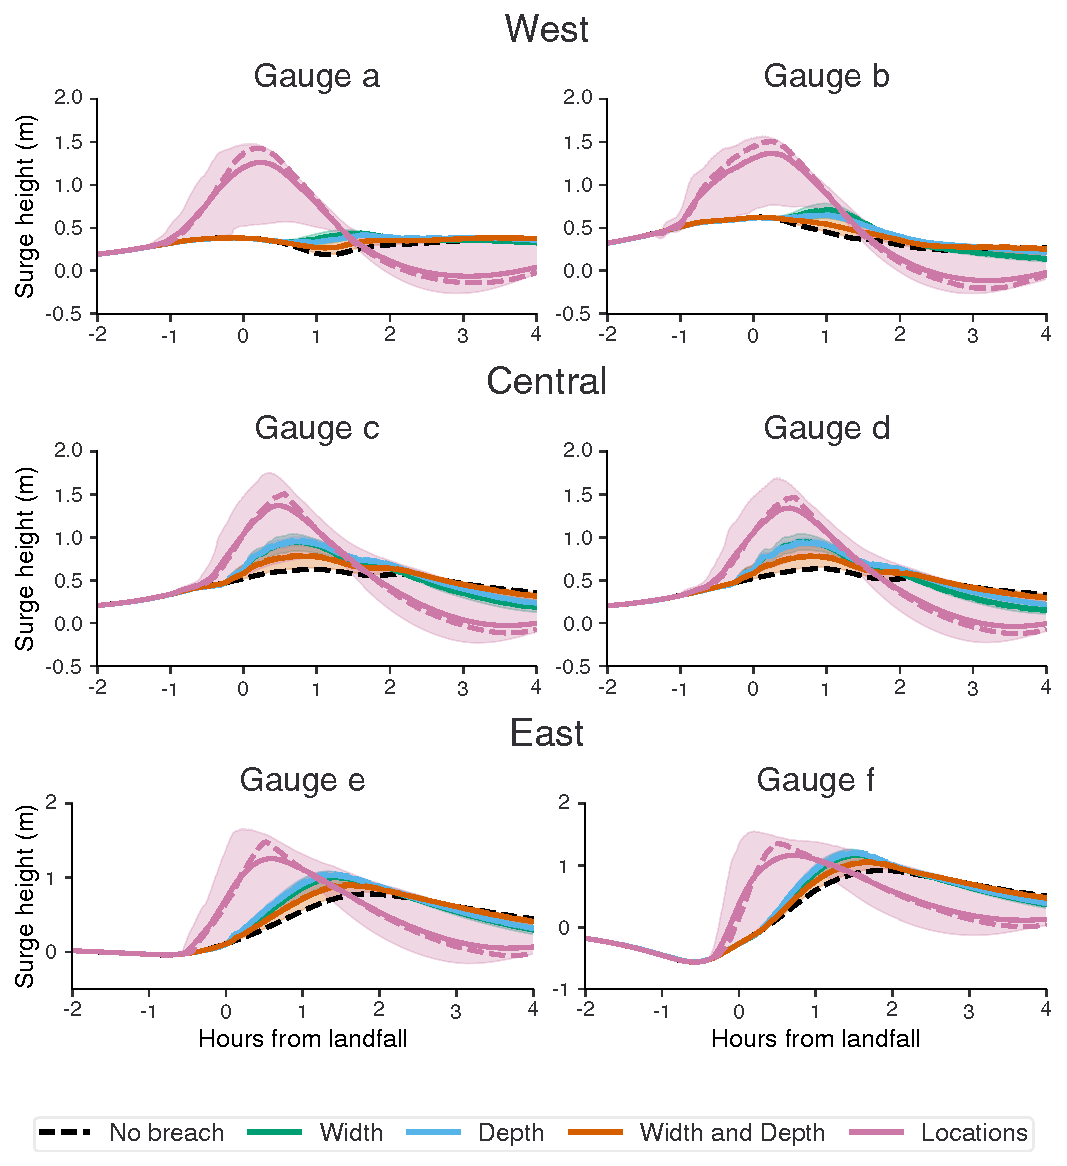
\includegraphics[width=0.75\textwidth]{figures/fig4_v2.pdf}
    \caption{Synthetic tide gauges for each section of the bay. See Figure \ref{fig:1} for locations. Each dark line is the mean of all of the simulations in that category, the dotted lines in each color represent the median of that category. Each shaded area covers the 5 - 95 percentile of the category}
    \label{fig:4}
\end{figure}

In all three sections of the bay the peak surge arrives earlier in the \emph{Location} scenarios. The peak surge for the west gauge 'a' arrives at  94 minutes, 99 minutes, 209 minutes, 13 minutes after the storm made landfall for the following scenarios respectively \emph{Width}, \emph{Depth}, \emph{Width and Depth}, \emph{Location}. West gauge 'b' peak surge is calculated to arrive at 60 minutes, 58 minutes, 5 minutes, and 15 minutes for \emph{Width}, \emph{Depth}, \emph{Width and Depth}, \emph{Location}. The central gauges have very similar surge patterns with peak surge occurring 42/42 minutes, 42/43 minutes, 49/48 minutes, and 28/29 minutes for each scenario and c/d gauges. Lastly, the eastern gauges peak surge arrives at 85/93 minutes, 82/91 minutes, 97/100 minutes, and 35/42 minutes for gauges e/f. The west and central regions the maximum surge for the \emph{Location} simulations is larger by several factors than the other scenarios, while the eastern gauges maximum surge is more even across scenarios. All of the breaching simulations differ from the no breach case.

Figure \ref{fig:5} illustrates the relationship between total breach area ($km^2$) and total inundation change from a no breach simulation. The relationship shows a logarithmic trend that starts with a minimum inundation of 0.1632 km$^2$ and illustrates that a larger breach area leads to more inundation to a point, around 75 possible breaches the curve levels off at a total breach area of 0.035 km$^2$ and an inundation change around 40.1 km$^2$. Inundation change grows more slowly beyond this point to a maximum total inundation of 49.06 km$^2$.

\begin{figure}[ht]
    \centering
    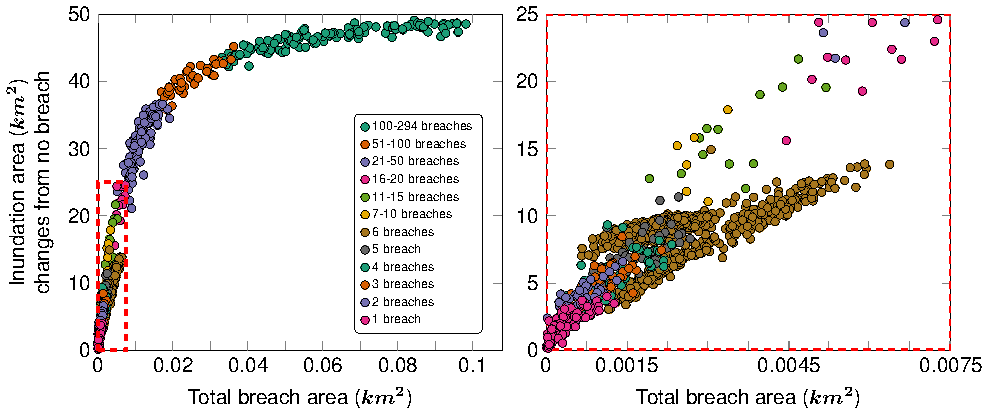
\includegraphics[width=\textwidth]{figures/fig5_v2.pdf}
    \caption{a) Total inundation vs. total breach size for all 1500 scenarios, points are colored per number of breaches. b) zoom in of a) panel to show differentiation of breach area and number of breaches and how the inundation can vary}
    \label{fig:5}
\end{figure}

\section{Discussion}
The results of this study illustrate that location, size, and number of breaches have an impact on coastal flooding. There is a clear relationship between total breach area and the amount of flooding in the bay and on the mainland coastline. The histograms plotted in Figure \ref{fig:3} illustrate a few different sections of the bay. The west surge point located near the Forge River mouth shows that given the original breaching locations the surge distribution is clustered and overlaps across scenarios, but when the simulations are allowed to vary breach locations the maximum surge is much higher from breaches located nearby. This location has surge pushed initially from the eastern side of the bay and after landfall the surge is pushed again from the western connection to Great South Bay and the nearby breaches.
The central location is adjacent to the mainland coastline near Seatuck Cove. Varying the breach locations and number of breaches increases the surge but to a smaller degree than in the west. The maximum surge at the central location is lower than in the west most likely due to proximity of the inlet. The peak surge that comes from more breaches in the west gets to the inlet before it reaches Seatuck Cove and allows the water to flood out of the bay reducing the maximum surge for this location. Additionally the shape of the coastline protects this location to some extent from surge coming from the southwest. 
The east location which is closest to the barrier island has the smallest maximum surge in the bay. Breaches formed eastward of the original locations do bring more surge to this location. However, its proximity to the inlet means that bay surge that travels towards the east after peak ocean surge is past, flows out of the inlet and reduces the total surge possible.

The gauges distributed in each section of the bay illustrate the differences of surge timing and maximum surge amongst the different scenarios as shown in Figure \ref{fig:4}. Many of the \emph{Location} simulations have breaches in the southwest portion of the barrier island. The peak ocean surge spreads from the southwest towards the northeast before landfall and the \emph{Location} breaches open earlier than the original breach locations due to this surge timing. This is shown in Figure \ref{fig:4} in the west gauges (a and b). The surge arrives earlier and is larger than the other simulations that have breaches closer to the inlet. The central gauges illustrate that while the surge is still larger, the timing is more in sync with the \emph{Depth}, \emph{Width}, and \emph{Width and Depth} scenarios. The eastern gauges maximum surge is not much higher than the other categories of simulations however the surge does still arrive earlier because of water coming into the bay from breaches in the southwest.

In Figure \ref{fig:5}a we show that the total breach dimensions have a relationship to the total area of inundation, with larger and more numerous breaches bringing more water inland. Total breach area across all breaches is the strongest predictor of greater coastal inundation, until the island is significantly eroded, then inundation growth slows considerably.
Figure \ref{fig:5}b brings more nuance to this relationship. While there appears to be a stronger correlation between breach width and inundation, than depth and inundation, breach depth's maximum of two meters is at least a factor of 20 smaller than total width for these scenarios, which reduces the impact depth can have on the hydrodynamics of each breach. The cluster of breaches that hover above the main grouping are the depth scenarios, whereas the width scenarios exhibit a more linear relationship with total inundation area.


\begin{figure}
    \centering
    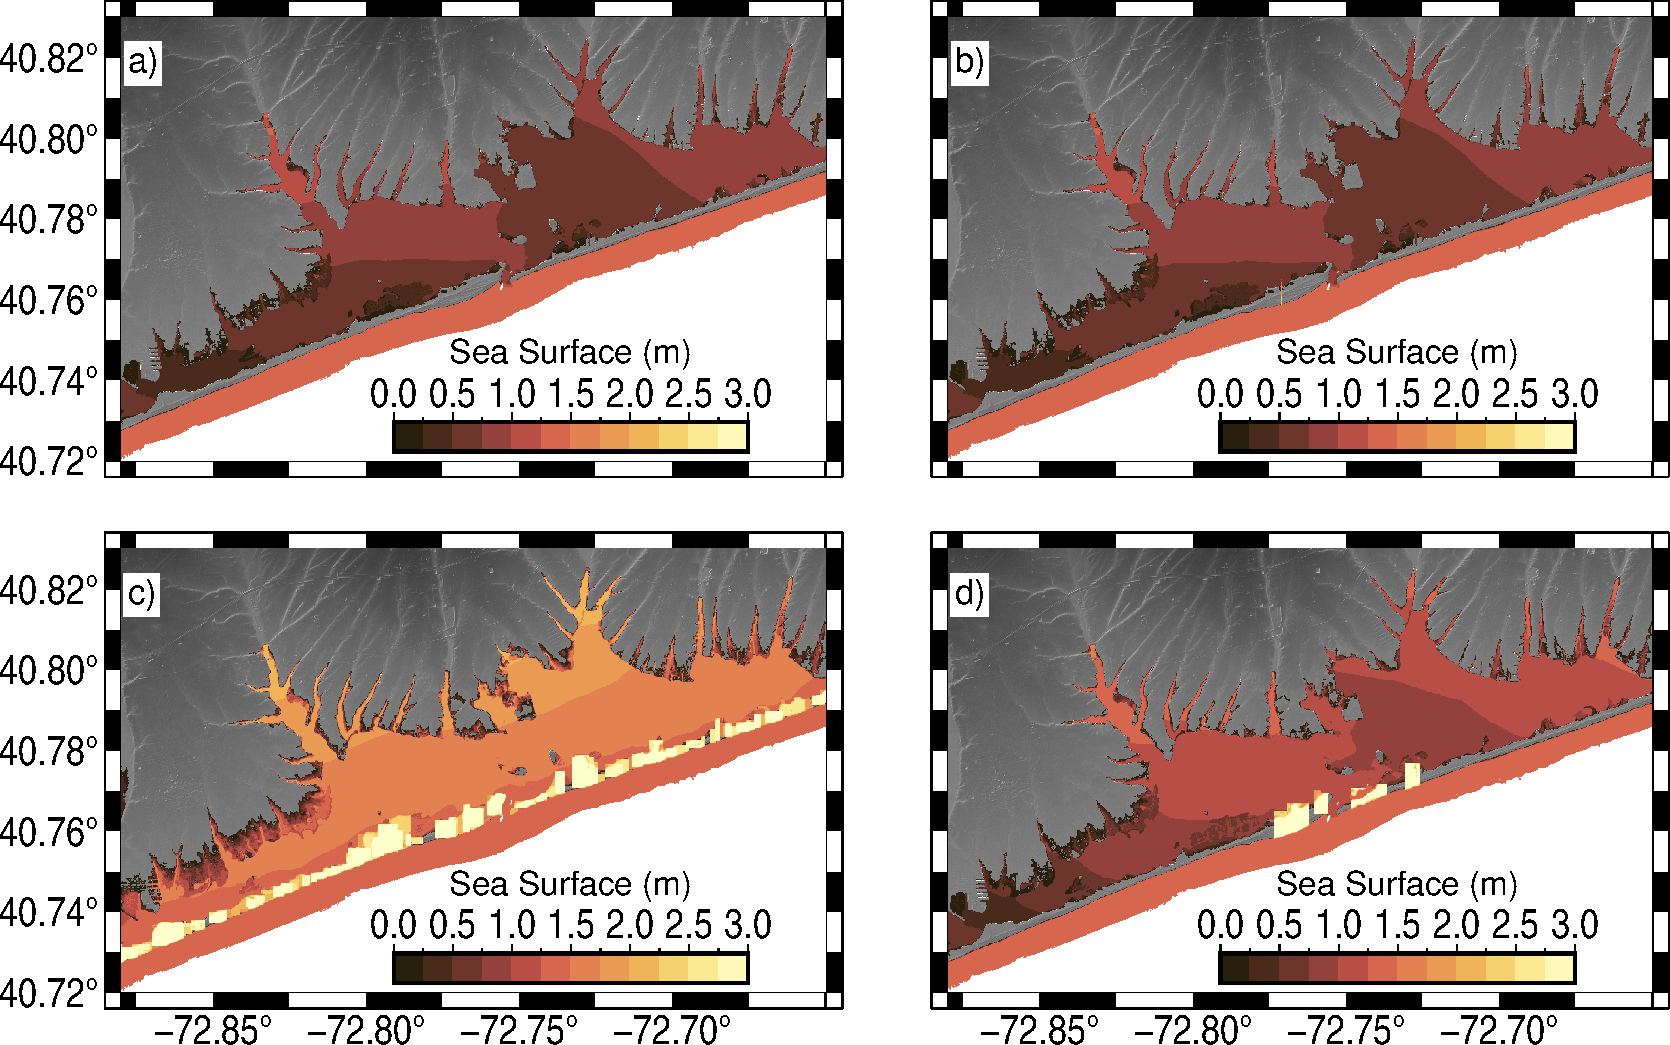
\includegraphics[width=0.85\textwidth]{figures/fig6_v2.pdf}

    \caption{Maps Moriches Bay, NY. Each panel is a separate simulation representing different values of storm surge inundation. Panel (a) is our No Breach scenario. Panel (b) is the minimum inundation of 0.162 $km^2$ with a single small breach. Panel (c) is the largest inundation scenario of 49.06 $km^2$ with 259 breaches. Panel (d)  is a simulation that has the closest inundation to the mean of all 1500 simulations 13.06 $km^2$, with six breaches.}
    \label{fig:6}
\end{figure}

Figure \ref{fig:6} illustrates that different inundation and bay surge patterns are correlated to number and size of breaches. Figure \ref{fig:6} panel a) is a no breach scenario which looks very similar in surge and inundation distribution to the minimum inundation (panel b) which has only a single small breach. There are approximately 500 different wet vs. dry cells between these two simulations, which is 163,200 square meters or .1632 square kilometers of inundation. Figure \ref{fig:6} panel d) is a simulation that comes closest to the mean of all the inundation change from all 1500 simulations. There are six medium to large sized breaches with a total breach area of .005 $km^2$ and total inundation change of 13.06 $km^2$. The simulation that comes closest to median of the scenarios (not pictured) has six medium sized breaches with a total inundation  The shape of the highs and lows of surge in the bay and the total horizontal coastal inundation is very different from the no breach or minimum inundation scenarios, with higher flooding potential in the coves, creeks and rivers that border the bay and along the lower elevation coastlines. Lastly the maximum inundation scenario is one where most of the island has been breached, this scenario has a bay surge of approximately two meters in most areas and the lowest elevation areas of the coastline are completely flooded.

The impact differing breach locations has on inundation as illustrated in Figure \ref{fig:6}b, can be further seen in Figure \ref{fig:7}. This figure shows the differences between two simulations with a similar total breach area, however the total inundation is very different. Figure \ref{fig:6}a, shows a scenario with six moderately sized breaches in the locations that occurred during the 1938 hurricane, the total breach area is .0039 $km^2$, and total inundation is 10.44 $km^2$. Figure \ref{fig:6}b, has a smaller total breach area of .0036 $km^2$ but a larger inundation at 12.03 $km^2$. The breaches in this scenario are generally smaller but more spaced out across the barrier island, with several in the western portion of the barrier island closer to Great South Bay. While the pattern of surge in the bay is similar it is visually different in the shape of the surge height and there is more coastal inundation along the western coastline. The Forge River surge is higher in Figure \ref{fig:6}b and the inlet region has a lower total water depth. The eastern portion of the bay has less inundation in \ref{fig:6}b, most likely due to the majority of the breaches being towards the west, plus the inlet allowing water to flow out of the bay.


\begin{figure}
    \centering
    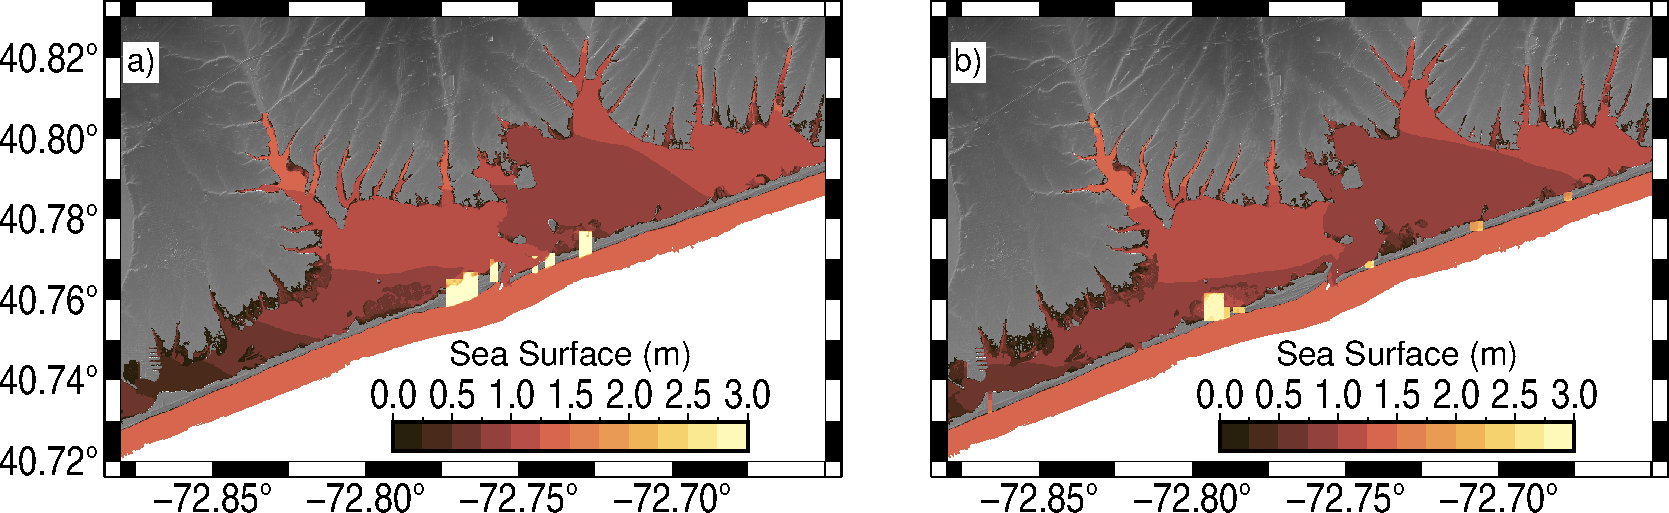
\includegraphics[width=0.95\textwidth]{figures/fig7_v2.pdf}
    \caption{a) Maximum surge and inundation for simulation that has 11 breaches and a total breach area of 0.0036 $km^2$. b) Maximum surge and inundation for simulations with 6 breaches and total breach area 0.0039 $km^2$}
    \label{fig:7}
\end{figure}


Figures \ref{fig:6} and \ref{fig:7} highlight the important details we discovered across our different simulations. Total breach area is a very strong predictor of total inundation. However, location of breaching is also very important, especially given the dynamics of the storm forcing and direction with which the surge is being pushed.

\section{Conclusions}
Breaching of a barrier island during a hurricane shows a strong impact on mainland inundation. The number, locations, and size of the breaches can change the inundation potential for the coastline. Understanding vulnerable areas and how breaching impacts them can provide opportunities for shoring up infrastructure and allowing planning that minimizes the storm's disruption to lives and the community.
Ideas for future work that can expand this study include; run many more simulations to find a better statistical distribution of the different breaching simulations. It will take a lot more data to find a consensus on specifically vulnerable locations, patterns of breaching, and its coastal impacts. Repeating simulations but varying the storms, will also provide insight into how the approach, speed, landfall location, and size of the storm affects the flooding and inundation. Performing many more simulations for other barrier islands, storms, and coastlines not only helps local communities plan for their own vulnerabilities but performing large scale simulations is valuable for expanding understanding of commonalities and differences of different regions.


\bibliography{ref}

\end{document}
